\documentclass[letterpaper,11pt,titlepage,openany,twoside,numbers=noenddot,bibliography=totoc,index=totoc]{scrbook}
\usepackage[dvips]{graphicx}
\usepackage[intoc]{nomencl}
\usepackage{phaistos}
\usepackage{amssymb}
\usepackage{amsmath}
\usepackage{amsthm}
\usepackage{empheq}
\usepackage[dvips]{xcolor}
\usepackage[english]{babel}
\usepackage{fancyhdr}
\usepackage{shadethm}
\usepackage{makeidx}
\usepackage{fouriernc,bm}
\usepackage[scaled=0.80]{beramono}
\usepackage[T1]{fontenc}
\usepackage{paralist}
\usepackage{mdwlist}
\usepackage{multicol}
\usepackage[font=small,labelfont=bf,labelsep=none,format=plain]{caption}
\usepackage{subfig}
\usepackage{tikz}
\usetikzlibrary{matrix}
\usepackage{picins}
\usepackage{framed}
\usepackage{nextpage}
\usepackage{listings}
\lstloadlanguages{Java}
\usepackage{jurabib}
\citeswithoutentry{arn,bow,cm,euc,hr,kam,kui,mtw,pc,rud,ste}
\bibliographystyle{jurabib}
\jurabibsetup{
 authorformat={smallcaps,and,firstnotreversed},
 titleformat={italic,commasep},
 commabeforerest,
 annote
}
\usepackage[pdfproducer={dvips + GPL Ghostscript 9.06},pdfcreator={LaTeX + dvips},
            pdfauthor={Michael Corral},pdftitle={Vector Calculus},
            pdfsubject={Calculus},pdfkeywords={calculus,vector},
            pdfdisplaydoctitle=true,dvips,bookmarks,pdfborder={0 0 0},
            bookmarksnumbered=true,colorlinks=false]{hyperref}
\usepackage{breakurl}
% Set sans serif font to Helvetica
\renewcommand\sfdefault{phv}
\newcommand{\startexercises}{
 \begin{center}\rule{\textwidth}{0.5pt}\end{center}
%%\centerline{\cornersize{1}\ovalbox{\textsf{\textbf{\large Exercises}}}} %embeds extra font
 \centerline{\fbox{\textsf{\textbf{\large Exercises}}}}
}
\newcommand{\probs}[1]{\par\noindent\textsf{\textbf{\large #1}}}
\setlength{\multicolsep}{2.5mm}
\setlength{\leftmargini}{1.4em}
\setlength{\shadeboxrule}{.4pt}
\theoremstyle{definition}
\newshadetheorem{defn}{Definition}[chapter]
\newshadetheorem{thm}{Theorem}[chapter]
\newshadetheorem{lem}[thm]{Lemma}
\newshadetheorem{cor}[thm]{Corollary}
\newtheoremstyle{itexmp}%
 {\topsep}
 {\topsep}
 {\normalfont}
 {0pt}
 {\itshape\bfseries}{.}
 { }
 {#1 \textit{#2}}
\theoremstyle{itexmp}
\newtheorem{exmp}{Example}[chapter]
\newcommand{\statedefn}[2]{
 \definecolor{shadethmcolor}{cmyk}{0.1,0.05,0,0}
 \definecolor{shaderulecolor}{cmyk}{0.73,0.19,0,0}
 \begin{defn}\label{#1}{#2}\end{defn}
}
\newcommand{\statethm}[2]{
% \definecolor{shadethmcolor}{HTML}{FFFF8B}
% \definecolor{shadethmcolor}{HTML}{DCC3FF}
 \definecolor{shadethmcolor}{HTML}{E8DCFF}
% \definecolor{shaderulecolor}{HTML}{FBC14D}
 \definecolor{shaderulecolor}{HTML}{9B5900}
 \begin{thm}\label{#1}{#2}\end{thm}
}
\newcommand{\statecor}[2]{
% \definecolor{shadethmcolor}{HTML}{FFFACD}
% \definecolor{shadethmcolor}{HTML}{FFD100}
 \definecolor{shadethmcolor}{HTML}{FFFF8B}
 \definecolor{shaderulecolor}{HTML}{9B5900}
 \begin{cor}\label{#1}{#2}\end{cor}
}
\newcommand{\statecomment}[2][0.96\textwidth]{
 \par\noindent\tikzstyle{mybox} = [draw=green!70!black,fill=green!5,thick,rectangle,rounded corners,inner ysep=4pt]
 \begin{tikzpicture}
  \node [mybox] (box){%
   \begin{minipage}{#1}{#2}\end{minipage}
  };
 \end{tikzpicture}
}
\newcommand\myclearpage{\cleartooddpage
 [\thispagestyle{empty}]}
\providecommand{\abs}[1]{\lvert\mspace{1mu}#1\mspace{1mu}\rvert}
\providecommand{\Abs}[1]{\bigl\lvert\mspace{1mu}#1\mspace{1mu}\bigr\rvert}
\providecommand{\norm}[1]{\lVert\mspace{1mu}#1\mspace{1mu}\rVert}
\providecommand{\Norm}[1]{\bigl\lVert\mspace{1mu}#1\mspace{1mu}\bigr\rVert}
\providecommand{\NORM}[1]{\Biggl\lVert\mspace{1mu}#1\mspace{1mu}\Biggr\rVert}
\providecommand{\ssub}[2]{#1_{\scriptscriptstyle #2}}
\providecommand{\vectwo}[1]{(#1_{\scriptscriptstyle 1},#1_{\scriptscriptstyle 2})}
\providecommand{\vectwoadd}[2]{(#1_{\scriptscriptstyle 1} + #2_{\scriptscriptstyle 1},
#1_{\scriptscriptstyle 2} + #2_{\scriptscriptstyle 2})}
\providecommand{\vectwosub}[2]{(#1_{\scriptscriptstyle 1} - #2_{\scriptscriptstyle 1},
#1_{\scriptscriptstyle 2} - #2_{\scriptscriptstyle 2})}
\providecommand{\vecthree}[1]{(#1_{\scriptscriptstyle 1},#1_{\scriptscriptstyle 2},#1_{\scriptscriptstyle 3})}
\providecommand{\vecthreeadd}[2]{(#1_{\scriptscriptstyle 1} + #2_{\scriptscriptstyle 1},
#1_{\scriptscriptstyle 2} + #2_{\scriptscriptstyle 2},#1_{\scriptscriptstyle 3} + #2_{\scriptscriptstyle 3})}
\providecommand{\vecthreesub}[2]{(#1_{\scriptscriptstyle 1} - #2_{\scriptscriptstyle 1},
#1_{\scriptscriptstyle 2} - #2_{\scriptscriptstyle 2},#1_{\scriptscriptstyle 3} - #2_{\scriptscriptstyle 3})}
\providecommand{\ssubsum}[3]{#1_{\scriptscriptstyle #3} + #2_{\scriptscriptstyle #3}}
\providecommand{\vecthreeijk}[1]{\ssub{#1}{1}\,\textbf{i} + \ssub{#1}{2}\,\textbf{j} + \ssub{#1}{3}\,\textbf{k}}
\providecommand{\Real}[1]{\mathbb{R}^{#1}}
\providecommand{\Dotprod}[2]{#1 \bm{\cdot} #2}
\providecommand{\Crossprod}[2]{#1 \bm{\times} #2}
\providecommand{\Degrees}[0]{\ensuremath{^\circ}}
\providecommand{\ival}[2]{\lbrack #1,#2 \rbrack}
\providecommand{\lineintvec}[3]{\int_{#1} \Dotprod{\textbf{#2}}{d\textbf{#3}}}
\providecommand{\olineintvec}[3]{\oint_{#1} \Dotprod{\textbf{#2}}{d\textbf{#3}}}
\newenvironment{proofbar}{%
  \def\FrameCommand{\vrule width 1pt \hspace{5pt}}%
  \MakeFramed {\advance\hsize-\width \FrameRestore}}%
 {\endMakeFramed}
\allowdisplaybreaks[1]
\numberwithin{figure}{section}
\setlength\oddsidemargin{20pt}
\setlength\evensidemargin{20pt}
\setlength\topmargin{0pt}

% Define \clockint and \counterint line integral symbols
\def\Xint#1{\mathchoice
 {\XXint\displaystyle\textstyle{#1}}%
 {\XXint\textstyle\scriptstyle{#1}}%
 {\XXint\scriptstyle\scriptscriptstyle{#1}}%
 {\XXint\scriptscriptstyle\scriptscriptstyle{#1}}%
 \!\int}
\def\XXint#1#2#3{{\setbox0=\hbox{$#1{#2#3}{\int}$}
 \vcenter{\hbox{$#2#3$}}\kern-.5\wd0}}
\def\clockint{\Xint\circlearrowright}
\def\counterint{\Xint\rotcirclearrowleft}
\def\rotcirclearrowleft{\mathpalette{\RotLSymbol{-30}}\circlearrowleft}
\def\RotLSymbol#1#2#3{\rotatebox[origin=c]{#1}{$#2#3$}}	
% End definition of \clockint and \counterint line integral symbols

\makeindex
\makenomenclature
\begin{document}
\deffootnote[1em]{0em}{1em}{\textsuperscript{\thefootnotemark}}
\frontmatter
\pagestyle{empty}
%Put the front cover here
%\centerline{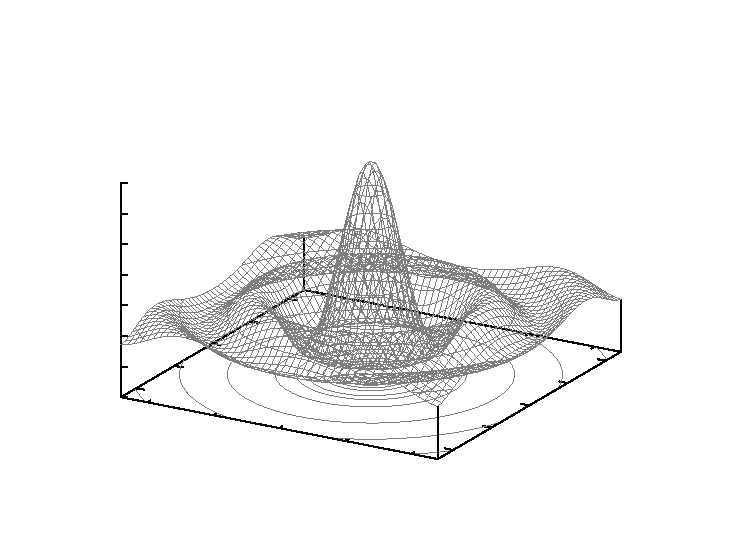
\includegraphics[height=0.3\textheight]{sincplain.eps}}\vspace{-25mm}
\centerline{\input{sincplaincover}}\vspace{-25mm}
\centerline{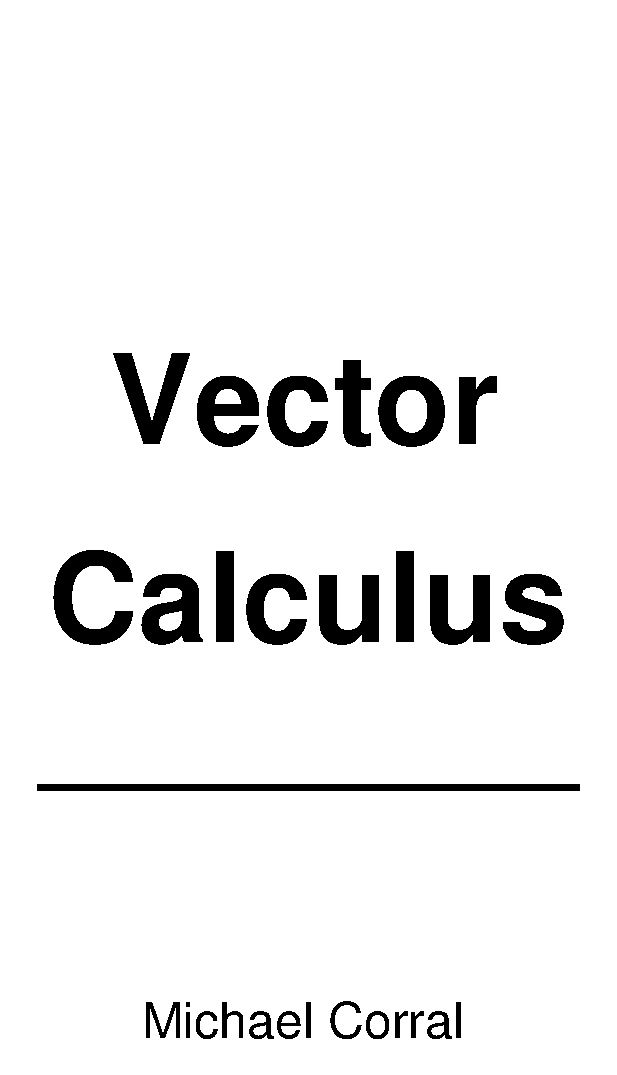
\includegraphics[height=0.6\textheight]{calc3bookcover}}
%Put the title page here
\title{Vector Calculus}
\author{\textsf{\textbf{Michael Corral}}}
\date{\large \textsf{\textsl{Schoolcraft College}}}
%Put the author/copyright info here
\uppertitleback{\emph{About the author}:\\
Michael Corral is an Adjunct Faculty member of the Department of Mathematics at Schoolcraft College. 
He received a B.A. in Mathematics from the University of California at Berkeley, and received an M.A. in Mathematics and
an M.S. in Industrial \& Operations Engineering from the University of Michigan.\\\\
This text was typeset in \LaTeXe\medspace with the \textsf{KOMA-Script} bundle, using the GNU Emacs text editor on a
Fedora Linux system. The graphics were created using MetaPost, PGF, and Gnuplot.}
\lowertitleback{Copyright \copyright ~2008 ~Michael Corral.\\
Permission is granted to copy, distribute and/or modify this document
under the terms of the GNU Free Documentation License, Version 1.2
or any later version published by the Free Software Foundation;
with no Invariant Sections, no Front-Cover Texts, and no Back-Cover
Texts. A copy of the license is included in the section entitled ``GNU
Free Documentation License''.}
\maketitle
\pagestyle{fancy}
\renewcommand{\sectionmark}[1]{\markright{\thesection\ #1}}
\renewcommand{\biblnfont}{\textnormal}
\renewcommand{\bibfnfont}{\textnormal}
\renewcommand{\bibtfont}{\textit}
\renewcommand{\bibansep}{, }
\renewcommand{\bibatsep}{,}
\renewcommand{\bibbdsep}{,}
\renewcommand{\qedsymbol}{\textsf{\textbf{\textsc{\footnotesize{QED}}}}}
\fancyhf{}
\fancyhead[LE]{\sffamily\bfseries\thepage}
\fancyhead[CE]{\sffamily\bfseries\leftmark}
\fancyhead[CO]{\sffamily\bfseries\rightmark}
\fancyhead[RO]{\sffamily\bfseries\thepage}
%Put the preface here
\addchap{Preface}
This book covers calculus in two and three variables. It is suitable for a one-semester course, normally known as
``Vector Calculus'', ``Multivariable Calculus'', or simply ``Calculus III''. 
The prerequisites are the standard courses
in single-variable calculus (also known as Calculus I and II).

The exercises are divided into three categories: A, B and C. 
The A exercises are mostly
of a routine computational nature, the B exercises are slightly more involved, and the C exercises usually require
some effort or insight to solve. 
A crude way of describing A, B and C would be ``Easy'', ``Moderate'' and ``Challenging'', respectively. 
However, many of the B exercises are easy and not all
the C exercises are difficult.

Answers and hints to most odd-numbered and some even-numbered exercises are
provided in Appendix A. 

There are a few exercises that require the student to write a computer program,
for example, the Monte Carlo method for approximating multiple integrals, in
Section \ref{sec:Numerical Approximation of Multiple Integrals}.
The code samples in the text are in the Java programming language, hopefully with enough comments so that the reader can
figure out what is being done even without knowing Java. Those exercises do not mandate the use of Java, so
students are free to implement the solutions using the language of their choice. While it would have been simple to
use a scripting language like Python, and perhaps even easier with a functional programming language (such as Haskell or Scheme), 
Java was chosen due to its ubiquity, relatively clear syntax, and easy availability for multiple platforms.

This book is released under the GNU Free Documentation License (GFDL), which allows others to not only copy and
distribute the book but also to modify it. 
For more details, see the included copy of the GFDL. So that there is no
ambiguity on this matter, anyone can make as many copies of this book as desired and distribute it as desired,
without needing a permission.

This book can be downloaded at \url{https://github.com/anton-petrunin/calc3book};
the older, original version by Michael Corral,
can be also obtained from \url{http://www.mecmath.net}. 

\pdfbookmark[0]{\contentsname}{toc}
%Put the table of contents here
\tableofcontents
\mainmatter
%Put the main chapters here
\chapter{Vectors in Euclidean Space}
%Begin Section 1.1
\section{Introduction}
In single-variable calculus, the functions that one encounters are functions of a variable (usually $x$ or $t$) 
that varies over some subset of the real number line (which we denote by $\mathbb{R}$).  For such a function, say,
$y = f(x)$, the \textbf{graph} of the function $f$ consists of the points $(x, y) = (x, f(x))$.  These points lie in
the \textbf{Euclidean plane}\index{plane!Euclidean}, which, in the \textbf{Cartesian}\index{coordinates} or
\textbf{rectangular}\index{coordinates!rectangular} coordinate system, consists\index{function}
of all ordered pairs of real numbers $(a, b)$.  We use the word ``Euclidean'' to denote a system in which all the
usual rules of Euclidean geometry hold.  We denote the Euclidean plane by $\Real{2}$\index{$\Real{2}$};
the ``2'' represents\index{coordinates!Cartesian}
the number of \emph{dimensions} of the plane.  The Euclidean plane has two perpendicular
\textbf{coordinate axes}: the $x$-axis and the $y$-axis.

In vector (or multivariable) calculus, we will deal with functions of two or three variables (usually $x, y$ or
$x, y, z$, respectively).  
The graph of a function of two variables, say, $z = f(x,y)$, lies in \textbf{Euclidean space}\index{Euclidean space}, which in the Cartesian coordinate system consists of all ordered
triples of real numbers $(a, b, c)$.  Since Euclidean space is 3-dimensional, we denote it by
$\Real{3}$\index{$\Real{3}$}.  The graph of $f$ consists
of the points $(x, y, z) = (x, y, f(x, y))$.  The 3-dimensional coordinate system of Euclidean space can be
represented on a flat surface, such as this page or a blackboard, only by giving the illusion of three
dimensions, in the manner shown in Figure \ref{fig:euc1}.  Euclidean space has three mutually perpendicular
coordinate axes ($x, y$ and $z$), and three mutually perpendicular coordinate planes\index{plane!coordinate}:
the $xy$-plane, $yz$-plane and $xz$-plane (see Figure \ref{fig:euc2}).
\newline
\begin{figure}[h]
\begin{minipage}[t]{7.5cm}
 \begin{center}
  \includegraphics{fig1.1.1.0}
 \end{center}
 \caption[]{}
 \label{fig:euc1}
\end{minipage}
\begin{minipage}[t]{7.5cm}
 \begin{center}
  \includegraphics{fig1.1.2.0}
 \end{center}
 \caption[]{}
 \label{fig:euc2}
\end{minipage}
\end{figure}

The coordinate system shown in Figure \ref{fig:euc1} is known as a
\textbf{right-handed coordinate system}\index{coordinates!right-handed}, because
it is possible, using the right hand, to point the index finger in the positive direction of the $x$-axis,
the middle finger in the positive direction of the $y$-axis, and the thumb in the positive direction of the
$z$-axis, as in Figure \ref{fig:rhs}.

\begin{figure}[h]
 \begin{center}
  %% Creator: Inkscape inkscape 0.48.1, www.inkscape.org
%% PDF/EPS/PS + LaTeX output extension by Johan Engelen, 2010
%% Accompanies image file 'righthand.eps' (pdf, eps, ps)
%%
%% To include the image in your LaTeX document, write
%%   \input{<filename>.pdf_tex}
%%  instead of
%%   \includegraphics{<filename>.pdf}
%% To scale the image, write
%%   \def\svgwidth{<desired width>}
%%   \input{<filename>.pdf_tex}
%%  instead of
%%   \includegraphics[width=<desired width>]{<filename>.pdf}
%%
%% Images with a different path to the parent latex file can
%% be accessed with the `import' package (which may need to be
%% installed) using
%%   \usepackage{import}
%% in the preamble, and then including the image with
%%   \import{<path to file>}{<filename>.pdf_tex}
%% Alternatively, one can specify
%%   \graphicspath{{<path to file>/}}
%% 
%% For more information, please see info/svg-inkscape on CTAN:
%%   http://tug.ctan.org/tex-archive/info/svg-inkscape

\begingroup
  \makeatletter
  \providecommand\color[2][]{%
    \errmessage{(Inkscape) Color is used for the text in Inkscape, but the package 'color.sty' is not loaded}
    \renewcommand\color[2][]{}%
  }
  \providecommand\transparent[1]{%
    \errmessage{(Inkscape) Transparency is used (non-zero) for the text in Inkscape, but the package 'transparent.sty' is not loaded}
    \renewcommand\transparent[1]{}%
  }
  \providecommand\rotatebox[2]{#2}
  \ifx\svgwidth\undefined
    \setlength{\unitlength}{277.909pt}
  \else
    \setlength{\unitlength}{\svgwidth}
  \fi
  \global\let\svgwidth\undefined
  \makeatother
  \begin{picture}(1,0.78089537)%
    \put(0,0){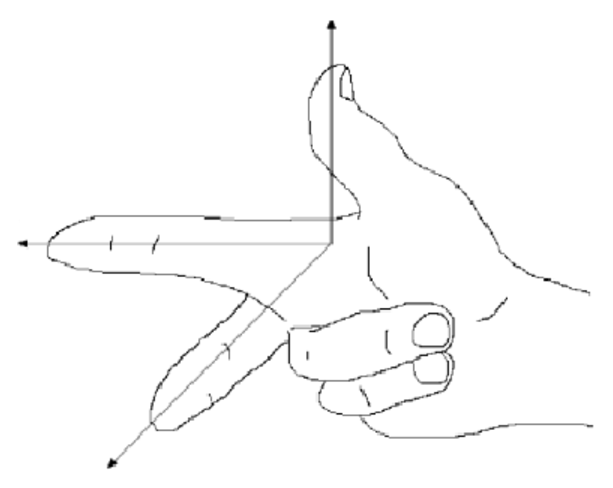
\includegraphics[width=\unitlength]{righthand.eps}}%
    \put(0.00631322,0.42986157){\color[rgb]{0,0,0}\makebox(0,0)[lb]{\smash{$x$}}}%
    \put(0.5863592,0.76090519){\color[rgb]{0,0,0}\makebox(0,0)[lb]{\smash{$z$}}}%
    \put(0.21069667,0.00814079){\color[rgb]{0,0,0}\makebox(0,0)[lb]{\smash{$y$}}}%
    \put(0.535983,0.33342713){\color[rgb]{0,0,0}\makebox(0,0)[lb]{\smash{0}}}%
  \end{picture}%
\endgroup

 \end{center}
 \caption[]{\quad Right-handed coordinate system.}
 \label{fig:rhs}
\end{figure}

An equivalent way of defining a right-handed system is if you can point your thumb upwards in the positive
$z$-axis direction while using the remaining four fingers to rotate the $x$-axis towards the $y$-axis.
Doing the same thing
with the left hand is what defines a \textbf{left-handed coordinate system}\index{coordinates!left-handed}.
Notice that switching the $x$- and $y$-axes
in a right-handed system results in a left-handed system, and that rotating either type of system does not change its
``handedness''.  Throughout the book we will use a right-handed system.

For functions of three variables, the graphs exist in 4-dimensional space (i.e. $\Real{4}$),
which we can not see in our 3-dimensional space, let alone simulate in 2-dimensional space.  So we
can only think of 4-dimensional space abstractly.  For an entertaining discussion of this subject, see the book by
\cite{abb}.\footnote{One thing you will learn is why a 4-dimensional creature would be able to reach inside an egg and
remove the yolk without cracking the shell!}

So far, we have discussed the \emph{position} of an object in 2-dimensional or 3-dimensional space.
But what about something such as the velocity\index{velocity} of the object, or its acceleration\index{acceleration}?
Or the gravitational force acting on the object? These phenomena all seem to involve motion and \emph{direction} in some
way.  This is where the idea of a \emph{vector} comes in.

You have already dealt with velocity and acceleration in single-variable calculus.  For example, for motion along a
straight line, if $y = f(t)$ gives the displacement of an object after time $t$, then $dy/dt = f\,'(t)$ is the velocity
of the object at time $t$.  The derivative\index{derivative}
$f\,'(t)$ is just a number, which is positive if the object is moving in an
agreed-upon ``positive'' direction, and negative if it moves in the opposite of that direction. So you can think of
that number, which was called the velocity of the object, as having two components: a \emph{magnitude}, indicated by
a nonnegative number, preceded by a \emph{direction}, indicated by a plus or minus symbol (representing motion in the
positive direction or the negative direction, respectively), i.e. $f\,'(t) = \pm a$ for some number $a \ge 0$.  Then
$a$ is the magnitude of the velocity (normally called the \emph{speed} of the object), and the $\pm$ represents the
direction of the velocity (though the $+$ is usually omitted for the positive direction).

For motion along a straight line, i.e. in a 1-dimensional space, the velocities are also contained in that 1-dimensional space, since they are just numbers.  
For general motion along a curve in 2- or 3-dimensional space,
however, velocity will need to be represented by a multidimensional object which should have both a magnitude and a
direction.  
A geometric object which has those features is an arrow, which in elementary geometry is called a
``directed line segment''.  This is the motivation for how we will define a vector\index{vector}.

\statedefn{defn:vec}{
 {A (nonzero) \textbf{vector} is a directed line segment drawn from a point $P$ (called its \textbf{initial point}) to
 a point $Q$ (called its \textbf{terminal point}), with $P$ and $Q$ being distinct points.  The vector is denoted by
 $\overrightarrow{PQ}$.  Its \textbf{magnitude} is the length of the line segment, denoted by
 $\Norm{\overrightarrow{PQ}}$, and its \textbf{direction} is the same as that of the directed line
 segment.  The \textbf{zero vector}\index{vector!zero} is just a point, and it is denoted by $\textbf{0}$.}
}

To indicate the direction\index{vector!direction} of a vector, we draw an arrow from its initial point to its terminal
point. We will often denote a vector by a single bold-faced letter (e.g. $\textbf{v}$) and use the terms
``magnitude''\index{vector!magnitude} and ``length'' interchangeably.
Note that our definition could apply to systems with any number of dimensions (see Figure \ref{fig:vecs}
(a)--(c)).

\begin{figure}[h]
 \centering
 \subfloat[][One dimension]{\includegraphics{fig1.1.4a.0}}
 \qquad
 \subfloat[][Two dimensions]{\includegraphics{fig1.1.4b.0}}
 \qquad
 \subfloat[][Three dimensions]{\includegraphics{fig1.1.4c.0}}
 \caption[]{\quad Vectors in different dimensions.}
 \label{fig:vecs}
\end{figure}

A few things need to be noted about the zero vector\index{vector!zero}.
Our motivation for what a vector is included the notions of
magnitude and direction. What is the magnitude of the zero vector? We define it to be zero, i.e.
$\norm{\textbf{0}} = 0$.
This agrees with the definition of the zero vector as just a point, which has zero length.  What about the
direction of the zero vector?  A single point really has no well-defined direction.  Notice that we were careful
to only define the direction of a \emph{nonzero} vector, which is well-defined since the initial and
terminal points are distinct.
Not everyone agrees on the direction of the zero vector.  Some contend that the zero vector has \emph{arbitrary}
direction (i.e. can take any direction), some say that it has \emph{indeterminate} direction (i.e. the direction can
not be determined), while others say that it has \emph{no} direction. Our definition of the zero vector, however,
does not require it to have a direction, and we will leave it at that.\footnote{In the subject of linear algebra
there is a more abstract way of defining a vector where the concept of ``direction'' is not really used.
See \cite{ar}.}

Now that we know what a vector is, we need a way of determining when two vectors are equal.  This leads us to the
following definition.
\statedefn{defn:equal}{
 {Two nonzero vectors are \textbf{equal} if they have the same magnitude and the same direction.  Any vector with zero
 magnitude is equal to the zero vector.}
}

By this definition, vectors with the same magnitude and direction but with different initial points would be
equal. For example, in Figure \ref{fig:veceq} the vectors \textbf{u}, \textbf{v} and \textbf{w} all have the same
magnitude $\sqrt 5$ (by the Pythagorean Theorem).  And we see that \textbf{u} and \textbf{w} are parallel, since they
lie on lines having the same slope $\frac{1}{2}$, and they point in the same direction. So $\textbf{u} = \textbf{w}$,
even though they have different initial points.  We also see that \textbf{v} is parallel to \textbf{u} but points in the
opposite direction. So $\textbf{u} \ne \textbf{v}$.

\begin{figure}[h]
 \begin{center}
  \includegraphics{fig1.1.5.0}
 \end{center}
 \caption[]{}
 \label{fig:veceq}
\end{figure}

So we can see that there are an infinite number of vectors for a given magnitude and direction, those vectors all
being equal and differing only by their initial and terminal points.  Is there a single vector which we can choose to
represent all those equal vectors?  The answer is yes, and is suggested by the vector \textbf{w} in Figure
\ref{fig:veceq}.

\statecomment{
 {Unless otherwise indicated, when speaking of ``the vector'' with a given magnitude and direction, we will mean the
  one whose initial point is at the origin of the coordinate system.}
}

\medskip
Thinking of vectors as starting from the origin provides a way of dealing with vectors in a standard way, since every
coordinate system has an origin.  But there
will be times when it is convenient to consider a different initial point for a vector (for example, when adding
vectors, which we will do in the next section).

Another advantage of using the origin as the initial point is that it provides an natural correspondence between a
vector and its terminal point.

\medskip
\hrule width \textwidth height 0.5pt
\begin{exmp}
 Let \textbf{v} be the vector in $\Real{3}$ whose initial point is at the origin and whose terminal point
 is $(3,4,5)$.  Though the \emph{point} $(3,4,5)$ and the vector \textbf{v} are different objects, it is
 convenient to write $\textbf{v} = (3,4,5)$.  When doing this, it is understood that the initial point of $\textbf{v}$
 is at the origin $(0,0,0)$ and the terminal point is $(3,4,5)$.
\end{exmp}

\begin{figure}[h]
 \centering
 \subfloat[][The point (3,4,5)]{\includegraphics{fig1.1.6a.0}}
 \qquad\qquad
 \subfloat[][The vector (3,4,5)]{\includegraphics{fig1.1.6b.0}}
 \caption[]{\quad Correspondence between points and vectors.}
 \label{fig:corresp}
\end{figure}
\hrule width \textwidth height 0.5pt
\medskip

Unless otherwise stated, when we refer to vectors as $\textbf{v} = (a,b)$ in $\Real{2}$ or $\textbf{v} = (a,b,c)$
in $\Real{3}$, we mean vectors in Cartesian coordinates starting at the origin.  Also, we will write
the zero vector $\textbf{0}$ in $\Real{2}$ and $\Real{3}$ as $(0,0)$ and $(0,0,0)$, respectively.

The point-vector correspondence provides a way to check if two vectors are equal, without having to determine their magnitude and direction.  
Similar to seeing if two points are the same, you are now seeing if the terminal points of vectors starting at the origin are the same.  
For each vector, find the (unique!) vector it equals whose initial point is the origin.  
Then compare the coordinates of the terminal points of these ``new'' vectors: 
if those coordinates are the same, then the original vectors are equal.  
To get the ``new'' vectors starting at the origin, you \emph{translate}\index{vector!translation}
each vector to start at the origin by subtracting the coordinates of the original
initial point from the original terminal point.  The resulting point will be the terminal point of
the ``new'' vector whose initial point is the origin.  Do this for each original vector then compare.

\begin{exmp}
 Consider the vectors $\overrightarrow{PQ}$ and $\overrightarrow{RS}$ in $\Real{3}$, where $P = (2,1,5),
 Q = (3,5,7), R = (1,-3,-2)$ and $S = (2,1,0)$.  Does $\overrightarrow{PQ} =
 \overrightarrow{RS}$?\\\emph{Solution:}
 The vector $\overrightarrow{PQ}$ is equal to the vector \textbf{v} with
 initial point $(0,0,0)$ and terminal point $Q - P = (3,5,7) - (2,1,5) = (3 - 2,5 - 1,7 - 5) = (1,4,2)$.
 \par\noindent
 Similarly, $\overrightarrow{RS}$ is equal to the vector \textbf{w} with
 initial point $(0,0,0)$ and terminal point $S - R = (2,1,0) - (1,-3,-2) = (2 - 1, 1 - (-3),0 - (-2)) = (1,4,2)$.
 \par\noindent
 So $\overrightarrow{PQ} = \textbf{v} = (1,4,2)$ and $\overrightarrow{RS} = \textbf{w} = (1,4,2)$.
 \par\noindent
 $\therefore \overrightarrow{PQ} = \overrightarrow{RS}$
\end{exmp}
\begin{figure}[h]
 \begin{center}
  \includegraphics{fig1.1.7.0}
 \end{center}
 \caption[]{}
 \label{fig:ex1.2}
\end{figure}
\hrule width \textwidth height 0.5pt
\medskip

Recall the distance\index{distance} formula for points in the Euclidean plane\index{distance!between points}:

\medskip
\statecomment{
 {For points $P = (\ssub{x}{1},\ssub{y}{1})$, $Q =
 (\ssub{x}{2},\ssub{y}{2})$ in $\Real{2}$, the distance $d$ between $P$ and $Q$ is:
  \begin{equation}
   d = \sqrt{(\ssub{x}{2} - \ssub{x}{1})^2 + (\ssub{y}{2} - \ssub{y}{1})^2}.
  \end{equation}}}
\medskip

By this formula, we have the following result:

\medskip
\statecomment{
 {For a vector $\overrightarrow{PQ}$ in $\Real{2}$ with initial point
  $P = (\ssub{x}{1},\ssub{y}{1})$ and terminal point\\
  $Q = (\ssub{x}{2},\ssub{y}{2})$, the magnitude of $\overrightarrow{PQ}$ is:
  \begin{equation}
   \Norm{\overrightarrow{PQ}} = \sqrt{(\ssub{x}{2} - \ssub{x}{1})^2 + (\ssub{y}{2} - \ssub{y}{1})^2}. 
   \label{eq:mag2}
  \end{equation}}}

Finding the magnitude of a vector $\textbf{v} = (a,b)$ in $\Real{2}$ is a
special case of formula (\ref{eq:mag2}) with $P = (0,0)$ and $Q = (a,b)$ :

\medskip
\statecomment{
 {For a vector $\textbf{v} = (a,b)$ in $\Real{2}$, the magnitude\index{vector!magnitude} of \textbf{v} is:
  \begin{equation}
   \norm{\textbf{v}} = \sqrt{a^2 + b^2}. 
   \label{eq:mag02}
  \end{equation}}}
\smallskip

To calculate the magnitude of vectors in $\Real{3}$, we need a distance formula for points in Euclidean
space\index{distance!between points} (we will postpone the proof until the next section):

\statethm{thm:dist3}{
 {The distance $d$ between points $P = (\ssub{x}{1},\ssub{y}{1},\ssub{z}{1})$ and
  $Q = (\ssub{x}{2},\ssub{y}{2},\ssub{z}{2})$ in $\Real{3}$ is:
  \begin{equation}
   d = \sqrt{(\ssub{x}{2} - \ssub{x}{1})^2 + (\ssub{y}{2} - \ssub{y}{1})^2 +
   (\ssub{z}{2} - \ssub{z}{1})^2}. 
   \label{eq:dist3}
  \end{equation}}
}
The proof will use the following result:
\statethm{thm:mag03}{
 {For a vector $\textbf{v} = (a,b,c)$ in $\Real{3}$, the magnitude\index{vector!magnitude} of \textbf{v} is:
  \begin{equation}
   \norm{\textbf{v}} = \sqrt{a^2 + b^2 + c^2}. 
   \label{eq:mag03}
  \end{equation}}
}
\begin{proofbar}\begin{proof}[Proof:]
 There are four cases to consider:
 \par\noindent\emph{Case 1: $a = b = c = 0$}.  Then $\textbf{v} = \textbf{0}$, so $\norm{\textbf{v}}
 = 0 = \sqrt{0^2 + 0^2 + 0^2} = \sqrt{a^2 + b^2 + c^2}$.
 \medskip
 \par\noindent\emph{Case 2: exactly two of $a, b, c$ are $0$.}  Without loss of generality, we assume that $a = b = 0$
 and $c \ne 0$ (the other two possibilities are handled in a similar manner).
 Then $\textbf{v} = (0,0,c)$, which is a vector of length $\abs{c}$ along the $z$-axis.
 So $\norm{\textbf{v}} = | c | = \sqrt{c^2} = \sqrt{0^2 + 0^2 + c^2} = \sqrt{a^2 + b^2 + c^2}$.
 \medskip
 \par\noindent\emph{Case 3: exactly one of $a, b, c$ is $0$.}  Without loss of generality, we assume that $a = 0$,
 $b \ne 0$ and $c \ne 0$ (the other two possibilities are handled in a similar manner).
 Then $\textbf{v} = (0,b,c)$, which is a vector in the $yz$-plane, so by the Pythagorean
 Theorem we have $\norm{\textbf{v}} = \sqrt{b^2 + c^2} = \sqrt{0^2 + b^2 + c^2} =
 \sqrt{a^2 + b^2 + c^2}$.
 \smallskip
 \piccaption[]{}\parpic[r]{\includegraphics{fig1.1.8.0}}
 \par\noindent\emph{Case 4: none of $a, b, c$ are $0$.}  Without loss of generality, we can assume that
 $a, b, c$ are all positive (the other seven possibilities are handled in a similar manner).
 Consider the points $P = (0,0,0)$, $Q = (a,b,c)$, $R =(a,b,0),$ and $S = (a,0,0)$, as shown in Figure 1.1.8. Applying
 the Pythagorean Theorem to the right triangle $\triangle PSR$ gives $\left\vert PR \right\vert^2 = a^2 + b^2$. A second
 application of the Pythagorean Theorem, this time to the right triangle $\triangle PQR$, gives $\norm{\textbf{v}}
 = \left\lvert PQ \right\rvert = \sqrt{\left\vert PR \right\vert^2 + \left\vert QR \right\vert^2} =
 \sqrt{a^2 + b^2 + c^2}$.\\
 This proves the theorem. \qquad \qedhere 
\end{proof}\end{proofbar}

\begin{exmp}
 Calculate the following:
 \begin{enumerate}[(a)]
  \item The magnitude of the vector $\overrightarrow{PQ}$ in $\Real{2}$ with $P = (-1,2)$ and
   $Q = (5,5)$.\\\emph{Solution:} By formula (\ref{eq:mag2}), $\Norm{\overrightarrow{PQ}} =
   \sqrt{(5 - (-1))^2 + (5 - 2)^2} = \sqrt{36 + 9} = \sqrt{45} = 3 \sqrt{5}$.
  \item The magnitude of the vector $\textbf{v} = (8,3)$ in $\Real{2}$.\\\emph{Solution:} By formula
   (\ref{eq:mag02}), $\norm{\textbf{v}} = \sqrt{8^2 + 3^2} = \sqrt{73}$.
  \item The distance between the points $P = (2, -1, 4)$ and $Q = (4, 2, -3)$ in $\Real{2}$.\\\emph{Solution:}
   By formula (\ref{eq:dist3}), the distance $d = \sqrt{(4 - 2)^2 + (2 - (-1))^2 + (-3 - 4)^2} =$\\$\sqrt{4 + 9 + 49} =
   \sqrt{62}$.
  \item The magnitude of the vector $\textbf{v} = (5,8,-2)$ in $\Real{3}$.\\\emph{Solution:} By formula
   (\ref{eq:mag03}), $\norm{\textbf{v}} = \sqrt{5^2 + 8^2 + (-2)^2} = \sqrt{25 + 64 + 4} = \sqrt{93}$.
 \end{enumerate}
\end{exmp}
\startexercises\label{sec1dot1}
\probs{A}
\begin{enumerate}[\bfseries 1.]
 \item Calculate the magnitudes of the following vectors:\\
  \begin{tabular}{@{} l l l l l @{}}
   (a) $\textbf{v} = (2,-1)$; & (b) $\textbf{v} = (2,-1,0)$; & (c) $\textbf{v} = (3,2,-2)$; & (d) $\textbf{v} = (0,0,1)$; &
   (e) $\textbf{v} = (6,4,-4)$.
  \end{tabular}
 \item For the points $P =(1,-1,1)$, $Q=(2,-2,2)$, $R=(2,0,1)$, $S=(3,-1,2)$, does $\overrightarrow{PQ} =
  \overrightarrow{RS}$?
 \item For the points $P =(0,0,0)$, $Q=(1,3,2)$, $R=(1,0,1)$, $S=(2,3,4)$, does $\overrightarrow{PQ} =
  \overrightarrow{RS}$?
\suspend{enumerate}
\probs{B}
\resume{enumerate}[{[\bfseries 1.]}]
 \item Let $\textbf{v} = (1,0,0)$ and $\textbf{w} = (a,0,0)$ be vectors in $\Real{3}$. Show that
 $\norm{\textbf{w}} = \abs{a} \,\norm{\textbf{v}}$.
 \item Let $\textbf{v} = (a,b,c)$ and $\textbf{w} = (3a,3b,3c)$ be vectors in $\Real{3}$. Show that
 $\norm{\textbf{w}}  = 3 \,\norm{\textbf{v}}$.
\suspend{enumerate}
\probs{C}
\resume{enumerate}[{[\bfseries 1.]}]
 \piccaption[]{}\parpic[r]{\includegraphics{fig1.1.9.0}}
 \item Though we will see a simple proof of Theorem \ref{thm:dist3} in the next section, it is possible to prove it using
 methods similar to those in the proof of Theorem \ref{thm:mag03}.  Prove the special case of Theorem \ref{thm:dist3}
 where the points $P = (\ssub{x}{1},\ssub{y}{1},\ssub{z}{1})$ and $Q = (\ssub{x}{2},\ssub{y}{2},\ssub{z}{2})$
 satisfy the following conditions:\\
 $\ssub{x}{2} > \ssub{x}{1} > 0$, $\ssub{y}{2} > \ssub{y}{1} > 0$, and
 $\ssub{z}{2} > \ssub{z}{1} > 0$.\\(\emph{Hint: Think of Case 4 in the proof of
 Theorem \ref{thm:mag03}, and consider Figure 1.1.9.})\\
\end{enumerate}

\newpage
%Begin Section 1.2
\section{Vector Algebra}
Now that we know what vectors are, we can start to perform some of the usual algebraic operations on them (e.g.
addition, subtraction). Before doing that, we will introduce the notion of a \emph{scalar}\index{scalar}.
\statedefn{defn:scal}{
 {A \textbf{scalar} is a quantity that can be represented by a single number.}
}
For our purposes, scalars will always be real numbers.\footnote{The term \emph{scalar} was invented by
19\textsuperscript{th} century
Irish mathematician, physicist and astronomer William Rowan Hamilton, to convey the sense of something
that could be represented by a point
on a scale or graduated ruler. The word vector comes from Latin, where it means ``carrier''.} Examples of
scalar quantities are mass, electric charge, and speed (not velocity).\footnote{An alternate definition of
scalars and vectors, used in physics, is that under certain types of coordinate transformations (e.g. rotations), a
quantity that is not affected is a scalar, while a quantity that is affected (in a certain way) is a vector.
See \cite{mar} for details.}
We can now define \emph{scalar multiplication} of a vector\index{vector!scalar multiplication}.

\statedefn{defn:scalmult}{
 {For a scalar $k$ and a nonzero vector \textbf{v}, the \textbf{scalar multiple} of \textbf{v} by $k$, denoted by
 $k\textbf{v}$, is the vector whose magnitude is $\abs{k} \,\norm{\textbf{v}}$, points in the same direction as
 \textbf{v} if $k > 0$, points in the opposite direction as \textbf{v} if $k < 0$, and is the zero vector $\textbf{0}$
 if $k = 0$. For the zero vector $\textbf{0}$, we define $k \textbf{0} = \textbf{0}$ for any scalar $k$.}
}

Two vectors \textbf{v} and \textbf{w} are \textbf{parallel}\index{vector!parallel} (denoted by $\textbf{v} \parallel
\textbf{w}$) if one is a scalar multiple of the other.
You can think of scalar multiplication of a vector as stretching or shrinking
the vector, and as flipping the vector in the opposite direction if the scalar is a negative number
(see Figure \ref{fig:scalar}).

\begin{figure}[h]
 \begin{center}
  \includegraphics{fig1.2.1.0}
 \end{center}
 \caption[]{}
 \label{fig:scalar}
\end{figure}

Recall that \textbf{translating}\index{vector!translation} a nonzero vector means that the initial point of the vector
is changed but the magnitude and direction are preserved. We are now ready to define
the \emph{sum}\index{vector!addition} of two vectors.

\statedefn{defn:vecsum}{
 {The \textbf{sum} of vectors \textbf{v} and \textbf{w}, denoted by $\textbf{v} + \textbf{w}$, is obtained by
 translating \textbf{w} so that its initial point is at the terminal point of \textbf{v}; the initial point of
 $\textbf{v} + \textbf{w}$ is the initial point of \textbf{v}, and its terminal point is the new terminal point of
 \textbf{w}.}
}

Intuitively, adding \textbf{w} to \textbf{v} means tacking on \textbf{w} to the end of \textbf{v} (see Figure
\ref{fig:sum}).

\begin{figure}[h]
 \centering
 \subfloat[][Vectors \textbf{v} and \textbf{w}]{\includegraphics{fig1.2.2a.0}}
 \qquad
 \subfloat[][Translate \textbf{w} to the end of \textbf{v}]{\includegraphics{fig1.2.2b.0}}
 \qquad
 \subfloat[][The sum $\textbf{v} + \textbf{w}$]{\includegraphics{fig1.2.2c.0}}
 \caption[]{\quad Adding vectors \textbf{v} and \textbf{w}.}
 \label{fig:sum}
\end{figure}

Notice that our definition is valid for the zero vector (which is just a point, and hence can be translated), and
so we see that $\textbf{v} + \textbf{0} = \textbf{v} = \textbf{0} + \textbf{v}$ for any vector \textbf{v}. In
particular, $\textbf{0} + \textbf{0} = \textbf{0}$. Also, it is easy to see that $\textbf{v} + (-\textbf{v}) =
\textbf{0}$, as we would expect. In general, since the scalar multiple $-\textbf{v} = -1 \,\textbf{v}$ is a
well-defined vector, we can define \textbf{vector subtraction}\index{vector!subtraction} as follows:
$\textbf{v} - \textbf{w} = \textbf{v} + (-\textbf{w})$. See Figure \ref{fig:subtract}.

\begin{figure}[h]
 \centering
 \subfloat[][Vectors \textbf{v} and \textbf{w}]{\includegraphics{fig1.2.3a.0}}
 \qquad
 \subfloat[][Translate $-\textbf{w}$ to the end of \textbf{v}]{\includegraphics{fig1.2.3b.0}}
 \qquad
 \subfloat[][The difference $\textbf{v} - \textbf{w}$]{\includegraphics{fig1.2.3c.0}}
 \caption[]{\quad Subtracting vectors \textbf{v} and \textbf{w}.}
 \label{fig:subtract}
\end{figure}

Figure \ref{fig:pgram} shows the use of ``geometric proofs'' of various laws of vector algebra, that is, it
uses laws from elementary geometry to prove statements about vectors.
For example, (a) shows that $\textbf{v} + \textbf{w} = \textbf{w} + \textbf{v}$ for any vectors $\textbf{v}$,
$\textbf{w}$. And (c) shows how you can think of $\textbf{v} - \textbf{w}$ as the vector that is tacked on to the end of
\textbf{w} to add up to \textbf{v}.

\begin{figure}[h]
 \centering
 \subfloat[][Add vectors]{\includegraphics{fig1.2.4a.0}}
 \qquad
 \subfloat[][Subtract vectors]{\includegraphics{fig1.2.4b.0}}
 \qquad
 \subfloat[][Combined add/subtract]{\includegraphics{fig1.2.4c.0}}
 \caption[]{\quad ``Geometric'' vector algebra.}
 \label{fig:pgram}
\end{figure}

Notice that we have temporarily abandoned the practice of starting vectors at the origin. In fact, we have not even
mentioned coordinates in this section so far. Since we will deal mostly with Cartesian coordinates in this book, the
following two theorems are useful for performing vector algebra on vectors in $\Real{2}$ and $\Real{3}$
starting at the origin.

\statethm{thm:cart2}{
 {Let $\textbf{v} = \vectwo{v}$, $\textbf{w} = \vectwo{w}$ be vectors in $\Real{2}$, and let $k$ be a scalar.
 Then\\(a)
 $k\textbf{v} = \vectwo{kv}$;
 \smallskip\\(b)
 $\textbf{v + w} = \vectwoadd{v}{w}$.}
}
\begin{proofbar}\begin{proof}[Proof:] (a)
 Without loss of generality, we assume that $\ssub{v}{1}, \ssub{v}{2} > 0$ (the other
 possibilities are handled in a similar manner). If $k = 0$ then $k\textbf{v} = 0\textbf{v} = \textbf{0} = (0,0)
 = \vectwo{0v} = \vectwo{kv}$, which
 is what we needed to show. If $k \ne 0$, then $\vectwo{kv}$ lies on a line
 with slope $\frac{\ssub{kv}{2}}{\ssub{kv}{1}} =
 \frac{\ssub{v}{2}}{\ssub{v}{1}}$, which is the same as the slope of the line on which
 \textbf{v} (and hence $k\textbf{v}$) lies, and $\vectwo{kv}$ points in the
 same direction on that line as $k\textbf{v}$.  Also, by formula (\ref{eq:mag02}) the magnitude of
 $\vectwo{kv}$ is $\sqrt{(\ssub{kv}{1})^2 +
 (\ssub{kv}{2})^2} = \sqrt{k^2 \ssub{v}{1}^2 + k^2 \ssub{v}{2}^2} = \sqrt{k^2 (\ssub{v}{1}^2 + \ssub{v}{2}^2)} =
 \abs{k} \,\sqrt{\ssub{v}{1}^2 + \ssub{v}{2}^2} = \abs{k} \,\norm{\textbf{v}}$.
 So $k\textbf{v}$ and $\vectwo{kv}$ have the same magnitude and direction.
 This proves (a).
 \smallskip
 
 \piccaption[]{}\parpic[r]{\includegraphics{fig1.2.5.0}}
 \par\noindent(b)
 Without loss of generality, we assume that $\ssub{v}{1}, \ssub{v}{2},
 \ssub{w}{1},\ssub{w}{2} > 0$ (the other possibilities are handled in a similar manner).
 From Figure 1.2.5, we see that when translating \textbf{w} to start at the end of \textbf{v}, the new
 terminal point of \textbf{w} is $\vectwoadd{v}{w}$, so by the definition of $\textbf{v} + \textbf{w}$ this must
 be the terminal point of $\textbf{v} + \textbf{w}$. 
 This proves (b).
\end{proof}\end{proofbar}
\statethm{thm:cart3}{
 {Let $\textbf{v} = \vecthree{v}$, $\textbf{w} = \vecthree{w}$ be vectors in $\Real{3}$, let $k$ be a scalar.
 Then\\
 (a) $k\textbf{v} = \vecthree{kv}$;
 \smallskip\\(b)
 $\textbf{v + w} = \vecthreeadd{v}{w}$.}
}
The following theorem summarizes the basic laws of vector algebra.
\statethm{thm:vecalg}{
 {For any vectors \textbf{u}, \textbf{v}, \textbf{w}, and scalars $k, l$,
 we have\par\noindent\begin{tabular}{@{} l r @{}}
 (a) $\textbf{v} + \textbf{w} = \textbf{w} + \textbf{v}$ & \qquad\qquad Commutative Law;
 \smallskip\\
 (b) $\textbf{u} + (\textbf{v} + \textbf{w}) = (\textbf{u} + \textbf{v}) + \textbf{w}$
 & \qquad\qquad Associative Law;
 \smallskip\\
 (c) $\textbf{v} + \textbf{0} = \textbf{v} = \textbf{0} + \textbf{v}$ & \qquad\qquad Additive Identity;
 \smallskip\\
 (d) $\textbf{v} +  (-\textbf{v}) = \textbf{0}$ & \qquad\qquad Additive Inverse;
 \smallskip\\
 (e) $k(l\textbf{v}) = (kl)\textbf{v}$ & \qquad\qquad Associative Law;
 \smallskip\\
 (f) $k(\textbf{v} + \textbf{w}) = k\textbf{v} + k\textbf{w}$ & \qquad\qquad Distributive Law;
 \smallskip\\
 (g) $(k + l)\textbf{v} = k\textbf{v} + l\textbf{v}$ & \qquad\qquad Distributive Law.
 \end{tabular}}
}
\begin{proofbar}\begin{proof}[Proof:]
 (a) We already presented a geometric proof of this in Figure \ref{fig:pgram}(a).
 \smallskip\\(b)
 To illustrate the difference between analytic proofs and geometric proofs in vector algebra, we will present both types
 here. For the analytic proof, we will use vectors in $\Real{3}$
 (the proof for $\Real{2}$ is similar).
 
 \par\noindent Let $\textbf{u} = \vecthree{u}$, $\textbf{v} = \vecthree{v}$, $\textbf{w} = \vecthree{w}$ be vectors in
 $\Real{3}$. Then
 \begin{alignat*}{2}
  \textbf{u} + (\textbf{v} + \textbf{w}) &= \vecthree{u} + (\vecthree{v} + \vecthree{w})\\
  &= \vecthree{u} + \vecthreeadd{v}{w} & &\text{~by Theorem \ref{thm:cart3}(b)}\\
  &= (\ssub{u}{1} + (\ssubsum{v}{w}{1}),\ssub{u}{2} + (\ssubsum{v}{w}{2}),\ssub{u}{3} + (\ssubsum{v}{w}{3})) &
      &\text{~by Theorem \ref{thm:cart3}(b)}\\
  &= ((\ssubsum{u}{v}{1}) + \ssub{w}{1},(\ssubsum{u}{v}{2}) + \ssub{w}{2},(\ssubsum{u}{v}{3}) + \ssub{w}{3}) &
      &\text{~by properties of real numbers}\\
  &= \vecthreeadd{u}{v} + \vecthree{w} & &\text{~by Theorem \ref{thm:cart3}(b)}\\
  &= (\textbf{u} + \textbf{v}) + \textbf{w}
 \end{alignat*}
 This completes the analytic proof of (b). Figure 1.2.6 provides the geometric proof.

 \piccaption[]{\quad Associative Law for vector addition}\parpic(\textwidth,0in){\includegraphics{fig1.2.6.0}
 \piccaptioninside}
 \par\mbox{}\newline\smallskip\picskip{0}
 
 \par\noindent(c) We already discussed this on p.10.\smallskip\\(d) We already discussed this on p.10.\smallskip\\(e)
 We will prove this for a vector $\textbf{v} = \vecthree{v}$ in $\Real{3}$ (the proof for
 $\Real{2}$ is similar):
 \begin{flalign*}
  \qquad k(l\textbf{v}) & = k\vecthree{lv} && \text{by Theorem \ref{thm:cart3}(a)}\qquad\qquad\qquad\qquad\qquad\\
  & = \vecthree{klv} && \text{by Theorem \ref{thm:cart3}(a)}\qquad\qquad\qquad\qquad\qquad\\
  & = (kl)\vecthree{v} && \text{by Theorem \ref{thm:cart3}(a)}\qquad\qquad\qquad\qquad\qquad\\
  & = (kl)\textbf{v}&
 \end{flalign*}
 
 \par\noindent(f) and (g): Left as exercises for the reader.
\end{proof}\end{proofbar}

A \textbf{unit vector}\index{vector!unit} is a vector with magnitude 1.
Notice that for any nonzero vector \textbf{v}, the vector $\frac{\textbf{v}}{\norm{\textbf{v}}}$ is a unit vector which
points in the same direction as \textbf{v}, since $\frac{1}{\norm{\textbf{v}}} > 0$ and
$\Norm{\frac{\textbf{v}}{\norm{\textbf{v}}}} = \frac{\norm{\textbf{v}}}{\norm{\textbf{v}}} = 1$. Dividing a nonzero
vector \textbf{v} by $\norm{\textbf{v}}$ is often called \emph{normalizing}\index{vector!normalized} \textbf{v}.

There are specific unit vectors which we will often use, called the \textbf{basis vectors}\index{vector!basis}:\\
$\textbf{i} = (1,0,0)$, $\textbf{j} = (0,1,0)$, and $\textbf{k} = (0,0,1)$ in $\Real{3}$;
$\textbf{i} = (1,0)$ and $\textbf{j} = (0,1)$ in $\Real{2}$. \\These are useful for several reasons: they are mutually
perpendicular, since they lie on distinct coordinate axes; they are all unit vectors: $\norm{\textbf{i}} =
\norm{\textbf{j}} = \norm{\textbf{k}} = 1$; every vector can be written as a unique scalar combination of the basis
vectors:\index{\textbf{i}, \textbf{j}, \textbf{k}}
$\textbf{v} = (a,b) = a\,\textbf{i} + b\,\textbf{j}$ in $\Real{2}$, $\textbf{v} = (a,b,c) = a\,\textbf{i} +
b\,\textbf{j} + c\,\textbf{k}$ in $\Real{3}$.\index{scalar!combination} See Figure \ref{fig:basis}.

\begin{figure}[h]
 \centering
 \subfloat[][$\Real{2}$]{\includegraphics{fig1.2.7a.0}}
 \quad
 \subfloat[][$\textbf{v} = a\,\textbf{i} + b\,\textbf{j}$]{\includegraphics{fig1.2.7b.0}}
 \quad
 \subfloat[][$\Real{3}$]{\includegraphics{fig1.2.7c.0}}
 \quad
 \subfloat[][$\textbf{v} = a\,\textbf{i} + b\,\textbf{j} + c\,\textbf{k}$]{\includegraphics{fig1.2.7d.0}}
 \caption[]{\quad Basis vectors in different dimensions.}
 \label{fig:basis}
\end{figure}

When a vector $\textbf{v} = (a,b,c)$ is written as $\textbf{v} = a\,\textbf{i} + b\,\textbf{j} + c\,\textbf{k}$, we say
that $\textbf{v}$ is in \emph{component form}\index{vector!components}, and that $a$, $b$, and $c$ are the
\emph{\textbf{i}, \textbf{j}, and \textbf{k} components}, respectively, of \textbf{v}. We have:
\begin{align*}
 \textbf{v} = \vecthreeijk{v}, k \text{~a scalar} &\Longrightarrow k\textbf{v} = \vecthreeijk{kv};\\
 \textbf{v} = \vecthreeijk{v}, \textbf{w} = \vecthreeijk{w} &\Longrightarrow \textbf{v} + \textbf{w} =
 (\ssubsum{v}{w}{1})\textbf{i} + (\ssubsum{v}{w}{2})\textbf{j} + (\ssubsum{v}{w}{3})\textbf{k};\\
 \textbf{v} = \vecthreeijk{v} &\Longrightarrow \norm{\textbf{v}} =
 \sqrt{\ssub{v}{1}^2 + \ssub{v}{2}^2 + \ssub{v}{3}^2}.
\end{align*}

\hrule width \textwidth height 0.5pt
\begin{exmp}
 Let $\textbf{v} = (2,1,-1)$ and $\textbf{w} = (3,-4,2)$ in $\Real{3}$.
 \begin{enumerate}[(a)]
  \item Find $\textbf{v} - \textbf{w}$.\\\emph{Solution:} $\textbf{v} - \textbf{w} =
   (2 - 3,1 - (-4), -1 - 2) = (-1,5,-3)$.
  \item Find $3\textbf{v} + 2\textbf{w}$.\\\emph{Solution:} $3\textbf{v} + 2\textbf{w} = (6,3,-3) + (6,-8,4) =
   (12,-5,1)$.
  \item Write \textbf{v} and \textbf{w} in component form.\\\emph{Solution:}
   $\textbf{v} = 2\,\textbf{i} + \textbf{j} - \textbf{k}$, $\textbf{w} = 3\,\textbf{i} - 4\,\textbf{j} + 2\,\textbf{k}$.
  \item Find the vector \textbf{u} such that $\textbf{u} + \textbf{v} = \textbf{w}$.\\\emph{Solution:} By Theorem
   \ref{thm:vecalg}, $\textbf{u} = \textbf{w} - \textbf{v} = -(\textbf{v} - \textbf{w}) = -(-1,5,-3) = (1,-5,3)$, by
   part(a).
  \item Find the vector \textbf{u} such that $\textbf{u} + \textbf{v} + \textbf{w} = \textbf{0}$.\\\emph{Solution:}
   By Theorem \ref{thm:vecalg}, $\textbf{u} = -\textbf{w} - \textbf{v} = -(3,-4,2) - (2,1,-1) = (-5,3,-1)$.
  \item Find the vector \textbf{u} such that $2\textbf{u} + \textbf{i} - 2\,\textbf{j} = \textbf{k}$.\\\emph{Solution:}
   $2\textbf{u} = -\textbf{i} + 2\,\textbf{j} + \textbf{k} \Longrightarrow \textbf{u} = -\frac{1}{2}\,\textbf{i} +
  \textbf{j} + \frac{1}{2}\,\textbf{k}$.
  \item Find the unit vector $\frac{\textbf{v}}{\norm{\textbf{v}}}$.\\\emph{Solution:}
   $\frac{\textbf{v}}{\norm{\textbf{v}}} = \frac{1}{\sqrt{2^2 + 1^2 + (-1)^2}} \,(2,1,-1) =
   \left ( \frac{2}{\sqrt{6}},\frac{1}{\sqrt{6}},\frac{-1}{\sqrt{6}} \right )$.
 \end{enumerate} 
\end{exmp}
\hrule width \textwidth height 0.5pt

We can now easily prove Theorem \ref{thm:dist3} from the previous section. The distance $d$ between two
points $P = (\ssub{x}{1},\ssub{y}{1},\ssub{z}{1})$ and $Q = (\ssub{x}{2},\ssub{y}{2},\ssub{z}{2})$ in $\Real{3}$ is the
same as the length of the vector $\textbf{w} - \textbf{v}$, where the vectors \textbf{v} and \textbf{w} are
defined as $\textbf{v} = (\ssub{x}{1},\ssub{y}{1},\ssub{z}{1})$
and $\textbf{w} = (\ssub{x}{2},\ssub{y}{2},\ssub{z}{2})$ (see Figure \ref{fig:dist3p}). So since $\textbf{w} -
\textbf{v} = (\ssub{x}{2} - \ssub{x}{1},\ssub{y}{2} - \ssub{y}{1},\ssub{z}{2} - \ssub{z}{1})$, then
$d = \norm{\textbf{w} - \textbf{v}} = \sqrt{(\ssub{x}{2} - \ssub{x}{1})^2 + (\ssub{y}{2} - \ssub{y}{1})^2 +
(\ssub{z}{2} - \ssub{z}{1})^2}$ by Theorem \ref{thm:mag03}.

\begin{figure}[h]
 \begin{center}
  \includegraphics{fig1.2.8.0}
 \end{center}
 \caption[]{\quad Proof of Theorem \ref{thm:mag03}: $d = \norm{\textbf{w} - \textbf{v}}$.}
 \label{fig:dist3p}
\end{figure}
\startexercises\label{sec1dot2}
\probs{A}
\begin{enumerate}[\bfseries 1.]
 \item Let $\textbf{v} = (-1,5,-2)$ and $\textbf{w} = (3,1,1)$.\smallskip\\
  \begin{tabular}{@{} l l l l @{}}
   (a) Find $\textbf{v} - \textbf{w}$. & (b) Find $\textbf{v} + \textbf{w}$. &
   (c) Find $\frac{\textbf{v}}{\norm{\textbf{v}}}$. &
   (d) Find $\Norm{\frac{1}{2}(\textbf{v} - \textbf{w})}$.\smallskip\\
   (e) Find $\Norm{\frac{1}{2}(\textbf{v} + \textbf{w})}$.\smallskip & (f) Find $-2\,\textbf{v} +
   4\,\textbf{w}$.\smallskip & (g) Find $\textbf{v} - 2\,\textbf{w}$.\\
   \multicolumn{3}{@{} l}{(h) Find the vector \textbf{u} such that $\textbf{u} + \textbf{v} + \textbf{w} =
   \textbf{i}$.}\smallskip\\
   \multicolumn{3}{@{} l}{(i) Find the vector \textbf{u} such that $\textbf{u} + \textbf{v} + \textbf{w} =
   2\,\textbf{j} + \textbf{k}$.}\smallskip\\
   \multicolumn{3}{@{} l}{(j) Is there a scalar $m$ such that $m(\textbf{v} + 2\,\textbf{w}) = \textbf{k}$? If so,
   find it.}
  \end{tabular}
 \item For the vectors $\textbf{v}$ and $\textbf{w}$ from Exercise 1, is $\norm{\textbf{v} - \textbf{w}} =
 \norm{\textbf{v}} - \norm{\textbf{w}}$? If not, which quantity is larger?
 \item For the vectors $\textbf{v}$ and $\textbf{w}$ from Exercise 1, is $\norm{\textbf{v} + \textbf{w}} =
 \norm{\textbf{v}} + \norm{\textbf{w}}$? If not, which quantity is larger?
\suspend{enumerate}
\probs{B}
\resume{enumerate}[{[\bfseries 1.]}]
 \begin{multicols}{2}
  \item Prove Theorem \ref{thm:vecalg}(f) for $\Real{3}$.
  \item Prove Theorem \ref{thm:vecalg}(g) for $\Real{3}$.
 \end{multicols}
\suspend{enumerate}
\probs{C}
\resume{enumerate}[{[\bfseries 1.]}]
 \item We know that every vector in $\Real{3}$ can be written as a scalar combination of the vectors \textbf{i},
 \textbf{j}, and \textbf{k}. Can every vector in $\Real{3}$ be written as a scalar combination of just \textbf{i} and
 \textbf{j}, i.e. for any vector \textbf{v} in $\Real{3}$, are there scalars $m$, $n$ such that $\textbf{v} =
 m\,\textbf{i} + n\,\textbf{j}$? Justify your answer.
\end{enumerate}


\newpage
%Begin Section 1.3
\section{Dot Product}
You may have noticed that while we did define multiplication of a vector by a scalar in the previous section on
vector algebra, we did not define multiplication of a vector by a vector. We will now see one type of
multiplication of vectors, called the \emph{dot product}\index{dot product}.

\statedefn{defn:dotprod}{
 {Let $\textbf{v} = \vecthree{v}$ and $\textbf{w} = \vecthree{w}$ be vectors in $\Real{3}$.\\The
 \textbf{dot product} of $\textbf{v}$ and $\textbf{w}$, denoted by $\Dotprod{\textbf{v}}{\textbf{w}}$, is given by:
 \begin{equation}
  \Dotprod{\textbf{v}}{\textbf{w}} = \ssub{v}{1}\ssub{w}{1} + \ssub{v}{2}\ssub{w}{2} + \ssub{v}{3}\ssub{w}{3}.
 \end{equation}
 Similarly, for vectors $\textbf{v} =\vectwo{v}$ and $\textbf{w} = \vectwo{w}$ in $\Real{2}$, the dot product is:
 \begin{equation}
  \Dotprod{\textbf{v}}{\textbf{w}} = \ssub{v}{1}\ssub{w}{1} + \ssub{v}{2}\ssub{w}{2}.
 \end{equation}}
}

Notice that the dot product of two vectors is a scalar, not a vector. 
So the associative law that holds for multiplication of numbers and for addition of vectors (see
Theorem \ref{thm:vecalg}(b),(e)), does \emph{not} hold for the dot product of vectors. Why? Because for vectors
$\textbf{u}$, $\textbf{v}$, $\textbf{w}$, the dot product $\Dotprod{\textbf{u}}{\textbf{v}}$ is a scalar, and so
$\Dotprod{(\Dotprod{\textbf{u}}{\textbf{v}})}{\textbf{w}}$ is not defined since the left side of that dot product
(the part in parentheses) is a scalar and not a vector.

For vectors $\textbf{v} = \vecthreeijk{v}$ and $\textbf{w} = \vecthreeijk{w}$ in component form, the dot product is
still $\Dotprod{\textbf{v}}{\textbf{w}} = \ssub{v}{1}\ssub{w}{1} + \ssub{v}{2}\ssub{w}{2} +
\ssub{v}{3}\ssub{w}{3}$.

Also notice that we defined the dot product in an analytic way, i.e. by referencing vector coordinates. There is
a geometric way of defining the dot product, which we will now develop as a consequence of the analytic
definition.

\statedefn{defn:vecangle}{
 {The \textbf{angle} between two nonzero vectors with the same initial point is the smallest angle between them.}
}

We do not define the angle between the zero vector and any other vector.
Any two nonzero vectors with the same initial point have two angles between them: $\theta$ and $360\Degrees - \theta$.
We will always choose the smallest nonnegative angle $\theta$ between them, so that $0\Degrees \leq \theta \leq
180\Degrees$\index{vector!angle between}.\index{angle} See Figure \ref{fig:angle}.

\begin{figure}[h]
 \centering
 \subfloat[][$0\Degrees < \theta < 180\Degrees$]{\includegraphics{fig1.3.1a.0}}
 \qquad
 \subfloat[][$\theta = 180\Degrees$]{\includegraphics{fig1.3.1b.0}}
 \qquad
 \subfloat[][$\theta = 0\Degrees$]{\includegraphics{fig1.3.1c.0}}
 \caption[]{\quad Angle between vectors.}
 \label{fig:angle}
\end{figure}

We can now take a more geometric view of
the dot product by establishing a relationship between the dot product of two vectors and the angle between them.

\statethm{thm:dotprod}{
 {Let $\textbf{v}$, $\textbf{w}$ be nonzero vectors, and let $\theta$ be the angle between them. Then
 \begin{equation}
  \cos \theta = \frac{\Dotprod{\textbf{v}}{\textbf{w}}}{\norm{\textbf{v}} \, \norm{\textbf{w}}} \label{eqn:dotprod}
 \end{equation}}
}
\begin{proofbar}\begin{proof}[Proof:]
 We will prove the theorem for vectors in $\Real{3}$ (the proof for $\Real{2}$ is similar). Let
 $\textbf{v} = \vecthree{v}$ and $\textbf{w} = \vecthree{w}$. 
 By the Law of Cosines (see Figure 1.3.2), we
 have
 \begin{equation}\label{eqn:cosines}
  \norm{\textbf{v} - \textbf{w}}^2 = \norm{\textbf{v}}^2 + \norm{\textbf{w}}^2 -
  2\,\norm{\textbf{v}}\,\norm{\textbf{w}} \cos \theta.
 \end{equation}
 (note that equation (\ref{eqn:cosines}) holds even for the ``degenerate'' cases $\theta = 0\Degrees$ and $180\Degrees)$.
 \piccaption[]{}\parpic(\textwidth,0in){\includegraphics{fig1.3.2.0}\piccaptioninside}
 \par\mbox{}\newline\smallskip\picskip{0}

 Since $\textbf{v} - \textbf{w} = \vecthreesub{v}{w}$, expanding $\norm{\textbf{v} - \textbf{w}}^2$
 in equation (\ref{eqn:cosines}) gives
 \begin{align*}
  \norm{\textbf{v}}^2 + \norm{\textbf{w}}^2 - 2\,\norm{\textbf{v}}\,\norm{\textbf{w}} \cos \theta &=
  (\ssub{v}{1} - \ssub{w}{1})^2 + (\ssub{v}{2} - \ssub{w}{2})^2 + (\ssub{v}{3} - \ssub{w}{3})^2\\
  &=
  (\ssub{v}{1}^2 - 2\ssub{v}{1}\ssub{w}{1} + \ssub{w}{1}^2) + (\ssub{v}{2}^2 - 2\ssub{v}{2}\ssub{w}{2} + \ssub{w}{2}^2)
  + (\ssub{v}{3}^2 - 2\ssub{v}{3}\ssub{w}{3} + \ssub{w}{3}^2)\\
  &= (\ssub{v}{1}^2 + \ssub{v}{2}^2 + \ssub{v}{3}^2) + (\ssub{w}{1}^2 + \ssub{w}{2}^2 + \ssub{w}{3}^2) -
  2(\ssub{v}{1}\ssub{w}{1} + \ssub{v}{2}\ssub{w}{2} + \ssub{v}{3}\ssub{w}{3})\\
  &=
  \norm{\textbf{v}}^2 + \norm{\textbf{w}}^2 - 2(\Dotprod{\textbf{v}}{\textbf{w}}) \text{~,~so}\\
  -2\,\norm{\textbf{v}}\,\norm{\textbf{w}} \cos \theta &= -2(\Dotprod{\textbf{v}}{\textbf{w}}) \text{~,~so since
  $\textbf{v} \ne \textbf{0}$ and $\textbf{w} \ne \textbf{0}$,}\\
  \cos \theta &= \frac{\Dotprod{\textbf{v}}{\textbf{w}}}{\norm{\textbf{v}} \, \norm{\textbf{w}}}.\qquad\qedhere
 \end{align*}
\end{proof}\end{proofbar}

\hrule width \textwidth height 0.5pt
\begin{exmp}
 Find the angle $\theta$ between the vectors $\textbf{v} = (2,1,-1)$ and $\textbf{w} =
 (3,-4,1)$.\smallskip
 \\\emph{Solution:}
 Since $\Dotprod{\textbf{v}}{\textbf{w}} = (2)(3) + (1)(-4) + (-1)(1) = 1$,
 $\norm{\textbf{v}} = \sqrt{6}$, and $\norm{\textbf{w}} = \sqrt{26}$, then
 \begin{displaymath}
  \cos \theta = \frac{\Dotprod{\textbf{v}}{\textbf{w}}}{\norm{\textbf{v}} \, \norm{\textbf{w}}} =
  \frac{1}{\sqrt{6}\,\sqrt{26}} = \frac{1}{2 \sqrt{39}} \approx 0.08 ~ \Longrightarrow ~ \theta \approx 85.41\Degrees.
 \end{displaymath}
\end{exmp}
\hrule width \textwidth height 0.5pt
\smallskip

Two nonzero vectors are \textbf{perpendicular}\index{vector!perpendicular} if the angle between them is $90\Degrees$.
Since $\cos 90\Degrees = 0$, we have the following important corollary to Theorem \ref{thm:dotprod}:

\statecor{cor:dotperp}{
 {Two nonzero vectors $\textbf{v}$ and $\textbf{w}$ are perpendicular if and only if $\Dotprod{\textbf{v}}{\textbf{w}} =
 0$.}
}
We will write $\textbf{v} \perp \textbf{w}$ to indicate that $\textbf{v}$ and $\textbf{w}$ are perpendicular.

Since $\cos \theta > 0$ for $0\Degrees \le \theta < 90\Degrees$ and $\cos \theta < 0$ for\index{vector!perpendicular}
$90\Degrees < \theta \le 180\Degrees$, we also have:

\statecor{cor:dotsign}{
 {If $\theta$ is the angle between nonzero vectors $\textbf{v}$ and $\textbf{w}$, then
 \begin{displaymath}
  \Dotprod{\textbf{v}}{\textbf{w}} \text{~~is~~}
  \begin{cases}
   > 0 & \text{for~~} 0\Degrees \le \theta < 90\Degrees,\\
   0 & \text{for~~} \theta = 90\Degrees,\\
   < 0 & \text{for~~} 90\Degrees < \theta \le 180\Degrees.
  \end{cases}
 \end{displaymath}}
}

By Corollary \ref{cor:dotsign}, the dot product can be thought of as a way of telling if the angle between two vectors
is acute, obtuse, or a right angle, depending on whether the dot product is positive, negative, or zero,
respectively. See Figure \ref{fig:dotsign}.

\begin{figure}[h]
 \centering
 \subfloat[][$\Dotprod{\textbf{v}}{\textbf{w}} > 0$]{\includegraphics{fig1.3.3a.0}}
 \qquad\qquad
 \subfloat[][$\Dotprod{\textbf{v}}{\textbf{w}} < 0$]{\includegraphics{fig1.3.3b.0}}
 \qquad\qquad
 \subfloat[][$\Dotprod{\textbf{v}}{\textbf{w}} = 0$]{\includegraphics{fig1.3.3c.0}}
 \caption[]{\quad Sign of the dot product \& angle between vectors.}
 \label{fig:dotsign}
\end{figure}

\hrule width \textwidth height 0.5pt
\begin{exmp}
 Are the vectors $\textbf{v} = (-1,5,-2)$ and $\textbf{w} = (3,1,1)$ perpendicular?\smallskip\\\emph{Solution:}
 Yes, $\textbf{v} \perp \textbf{w}$ since $\Dotprod{\textbf{v}}{\textbf{w}} = (-1)(3) + (5)(1) + (-2)(1) = 0$.
\end{exmp}
\hrule width \textwidth height 0.5pt
\medskip

The following theorem summarizes the basic properties of the dot product.

\statethm{thm:dotprop}{
 {For any vectors \textbf{u}, \textbf{v}, \textbf{w}, and scalar $k$,
 we have\par\noindent\begin{tabular}{@{} l r @{}}
 (a) $\Dotprod{\textbf{v}}{\textbf{w}} = \Dotprod{\textbf{w}}{\textbf{v}}$ & \qquad\qquad Commutative Law;\smallskip\\
 (b) $\Dotprod{(k\textbf{v})}{\textbf{w}} = \Dotprod{\textbf{v}}{(k\textbf{w})} = k(\Dotprod{\textbf{v}}{\textbf{w}})$
 & \qquad\qquad Associative Law;\smallskip\\
 (c) $\Dotprod{\textbf{v}}{\textbf{0}} = 0 = \Dotprod{\textbf{0}}{\textbf{v}}$;\smallskip\\
 (d) $\Dotprod{\textbf{u}}{(\textbf{v} + \textbf{w})} = \Dotprod{\textbf{u}}{\textbf{v}} +
 \Dotprod{\textbf{u}}{\textbf{w}}$ & \qquad\qquad Distributive Law;\smallskip\\
 (e) $\Dotprod{(\textbf{u} + \textbf{v})}{\textbf{w}} = \Dotprod{\textbf{u}}{\textbf{w}} +
 \Dotprod{\textbf{v}}{\textbf{w}}$ & \qquad\qquad Distributive Law;\smallskip\\
 (f) $\abs{\Dotprod{\textbf{v}}{\textbf{w}}} \le \norm{\textbf{v}}\,\norm{\textbf{w}}$ & \qquad\qquad
 Cauchy--Schwarz Inequality.\footnotemark\index{Cauchy--Schwarz Inequality}
 \end{tabular}}
}\footnotetext{Also known as the Cauchy--Schwarz--Buniakovski Inequality.}
\begin{proofbar}\begin{proof}[Proof:]
 The proofs of parts (a)--(e) are straightforward applications of the definition of the dot product, and are left
 to the reader as exercises. We will prove part (f).\\(f)
 If either $\textbf{v} = \textbf{0}$ or $\textbf{w} = \textbf{0}$, then $\Dotprod{\textbf{v}}{\textbf{w}} = 0$
 by part (c), and so the inequality holds trivially. So assume that \textbf{v} and \textbf{w} are nonzero vectors. Then
 by Theorem \ref{thm:dotprod},
 \begin{align*}
  \Dotprod{\textbf{v}}{\textbf{w}} &= \cos \theta \, \norm{\textbf{v}}\,\norm{\textbf{w}} \text{~,~so}\\
  \abs{\Dotprod{\textbf{v}}{\textbf{w}}} &= \abs{\cos \theta} \, \norm{\textbf{v}}\,\norm{\textbf{w}} \text{~,~so}\\
  \abs{\Dotprod{\textbf{v}}{\textbf{w}}} &\le \norm{\textbf{v}}\,\norm{\textbf{w}}
   \text{~~since $\abs{\cos \theta} \le 1$. \qquad \qedhere}
 \end{align*}
\end{proof}\end{proofbar}

Using Theorem \ref{thm:dotprop}, we see that if $\Dotprod{\textbf{u}}{\textbf{v}} = 0$ and
$\Dotprod{\textbf{u}}{\textbf{w}} = 0$, then 
\[\Dotprod{\textbf{u}}{(k\textbf{v} + l\textbf{w})} =
k(\Dotprod{\textbf{u}}{\textbf{v}}) + l(\Dotprod{\textbf{u}}{\textbf{w}}) = k(0) + l(0) =0\] for all scalars $k, l$.
Thus, we have the following fact:\smallskip
\statecomment{
 {\begin{center}If $\textbf{u} \perp \textbf{v}$ and $\textbf{u} \perp \textbf{w}$, then
  $\textbf{u} \perp (k\textbf{v} + l\textbf{w})$ for all scalars $k, l$.\end{center}}
}

\smallskip
For vectors \textbf{v} and \textbf{w}, the collection of all scalar combinations $k\textbf{v} + l\textbf{w}$
is called the \textbf{span} of \textbf{v} and \textbf{w}\index{span}. If nonzero vectors \textbf{v} and \textbf{w} are
parallel, then their span is a line; if they are not parallel, then their span is a plane. So what we showed above is
that a vector which is perpendicular to two other vectors is also perpendicular to their span.

The dot product can be used to derive properties of the magnitudes of vectors, the most important of which is the
\emph{Triangle Inequality}, as given in the following theorem:

\statethm{thm:dotnorm}{
 {For any vectors \textbf{v}, \textbf{w}, we have\par\noindent\begin{tabular}{@{} l r @{}}
  (a) $\norm{\textbf{v}}^2 = \Dotprod{\textbf{v}}{\textbf{v}}$;\\
  (b) $\norm{\textbf{v} + \textbf{w}} \le \norm{\textbf{v}} + \norm{\textbf{w}}$
   & \qquad\qquad Triangle Inequality\index{triangle inequality};\smallskip\\
  (c) $\norm{\textbf{v} - \textbf{w}} \ge \norm{\textbf{v}} - \norm{\textbf{w}}$.
 \end{tabular}}
}
\begin{proofbar}\begin{proof}[Proof:]
 (a) Left as an exercise for the reader.\smallskip\\(b) By part (a) and Theorem \ref{thm:dotprop}, we have
  \begin{align*}
   \norm{\textbf{v} + \textbf{w}}^2 &= \Dotprod{(\textbf{v} + \textbf{w})}{(\textbf{v} + \textbf{w})}
   = \Dotprod{\textbf{v}}{\textbf{v}} + \Dotprod{\textbf{v}}{\textbf{w}} + \Dotprod{\textbf{w}}{\textbf{v}} +
   \Dotprod{\textbf{w}}{\textbf{w}}\\
   &= \norm{\textbf{v}}^2 + 2(\Dotprod{\textbf{v}}{\textbf{w}}) + \norm{\textbf{w}}^2 \text{~, so since $a \le \abs{a}$
    for any real number $a$, we have}\\
   &\le \norm{\textbf{v}}^2 + 2\,\abs{\Dotprod{\textbf{v}}{\textbf{w}}} + \norm{\textbf{w}}^2 
    \text{~, so by Theorem \ref{thm:dotprop}(f) we have}\\
   &\le \norm{\textbf{v}}^2 + 2\,\norm{\textbf{v}}\,\norm{\textbf{w}} + \norm{\textbf{w}}^2 =
    (\norm{\textbf{v}} + \norm{\textbf{w}})^2 \text{~and so}\\
   \norm{\textbf{v} + \textbf{w}} &\le \norm{\textbf{v}} + \norm{\textbf{w}}
    \text{~after taking square roots of both sides, which proves (b).}
  \end{align*}
  \par\noindent(c) Since $\textbf{v} = \textbf{w} + (\textbf{v} - \textbf{w})$, then $\norm{\textbf{v}} = 
  \norm{\textbf{w} + (\textbf{v} - \textbf{w})} \le \norm{\textbf{w}} + \norm{\textbf{v} - \textbf{w}}$
  by the Triangle Inequality, so subtracting $\norm{\textbf{w}}$ from both sides gives
  $\norm{\textbf{v}} - \norm{\textbf{w}} \le \norm{\textbf{v} - \textbf{w}}$. \qquad \qedhere 
\end{proof}\end{proofbar}

\piccaption[]{}\parpic[r]{\includegraphics{fig1.3.4.0}}
\par The Triangle Inequality gets its name from the fact that in any triangle, no one side is longer than the sum of
the lengths of the other two sides (see Figure 1.3.4). Another way of saying this is with the familiar statement ``the
shortest distance between two points is a straight line.''


\startexercises\label{sec1dot3}
\probs{A}
\begin{enumerate}[\bfseries 1.]
 \item Let $\textbf{v} = (5,1,-2)$ and $\textbf{w} = (4,-4,3)$. Calculate $\Dotprod{\textbf{v}}{\textbf{w}}$.
 \item Let $\textbf{v} = -3\,\textbf{i} - 2\,\textbf{j} - \textbf{k}$ and
  $\textbf{w} = 6\,\textbf{i} + 4\,\textbf{j} + 2\,\textbf{k}$. Calculate $\Dotprod{\textbf{v}}{\textbf{w}}$.
\suspend{enumerate}
\par\noindent For Exercises \ref{ex:theta:first}--\ref{ex:theta:last}, find the angle $\theta$ between the vectors $\textbf{v}$ and $\textbf{w}$.
\resume{enumerate}[{[\bfseries 1.]}]
 \begin{multicols}{2}
  \item\label{ex:theta:first} $\textbf{v} = (5,1,-2)$, $\textbf{w} = (4,-4,3)$;
  \item $\textbf{v} = (7,2,-10)$, $\textbf{w} = (2,6,4)$;
 \end{multicols}
 \begin{multicols}{2}
  \item $\textbf{v} = (2,1,4)$, $\textbf{w} = (1,-2,0)$;
  \item $\textbf{v} = (4,2,-1)$, $\textbf{w} = (8,4,-2)$;
 \end{multicols}
 \begin{multicols}{2}
  \item $\textbf{v} = -\,\textbf{i} + 2\,\textbf{j} + \textbf{k}$,
   $\textbf{w} = -3\,\textbf{i} + 6\,\textbf{j} + 3\,\textbf{k}$;
  \item\label{ex:theta:last} $\textbf{v} = \textbf{i}$, $\textbf{w} = 3\,\textbf{i} + 2\,\textbf{j} + 4\textbf{k}$.
 \end{multicols}
 \item Let $\textbf{v} = (8,4,3)$ and $\textbf{w} = (-2,1,4)$. Is $\textbf{v} \perp \textbf{w}$? Justify your answer.
 \item Let $\textbf{v} = (6,0,4)$ and $\textbf{w} = (0,2,-1)$. Is $\textbf{v} \perp \textbf{w}$? Justify your answer.
 \item For $\textbf{v}$, $\textbf{w}$ from Exercise 5, verify the Cauchy--Schwarz Inequality
  $\abs{\Dotprod{\textbf{v}}{\textbf{w}}} \le \norm{\textbf{v}}\,\norm{\textbf{w}}$.
 \item For $\textbf{v}$, $\textbf{w}$ from Exercise 6, verify the Cauchy--Schwarz Inequality
  $\abs{\Dotprod{\textbf{v}}{\textbf{w}}} \le \norm{\textbf{v}}\,\norm{\textbf{w}}$.
 \item For $\textbf{v}$, $\textbf{w}$ from Exercise 5, verify the Triangle Inequality
  $\norm{\textbf{v} + \textbf{w}} \le \norm{\textbf{v}} + \norm{\textbf{w}}$.
 \item For $\textbf{v}$, $\textbf{w}$ from Exercise 6, verify the Triangle Inequality
  $\norm{\textbf{v} + \textbf{w}} \le \norm{\textbf{v}} + \norm{\textbf{w}}$.
\suspend{enumerate}
\probs{B}
\smallskip
\resume{enumerate}[{[\bfseries 1.]}]
 \begin{multicols}{2}
  \item Prove Theorem \ref{thm:dotprop}(a).
  \item Prove Theorem \ref{thm:dotprop}(b).
 \end{multicols}
 \begin{multicols}{2}
  \item Prove Theorem \ref{thm:dotprop}(c).
  \item Prove Theorem \ref{thm:dotprop}(d).
 \end{multicols}
 \begin{multicols}{2}
  \item Prove Theorem \ref{thm:dotprop}(e).
  \item Prove Theorem \ref{thm:dotnorm}(a).
 \end{multicols}
 \item Prove or give a counterexample: If $\Dotprod{\textbf{u}}{\textbf{v}} = \Dotprod{\textbf{u}}{\textbf{w}}$,
  then $\textbf{v} =\textbf{w}$.
\suspend{enumerate}
\probs{C}
\resume{enumerate}[{[\bfseries 1.]}]
 \item Prove or give a counterexample: If $\Dotprod{\textbf{v}}{\textbf{w}} = 0$ for all $\textbf{v}$, then
  $\textbf{w} =\textbf{0}$.
 \item Prove or give a counterexample: If $\Dotprod{\textbf{u}}{\textbf{v}} = \Dotprod{\textbf{u}}{\textbf{w}}$
  for all $\textbf{u}$, then $\textbf{v} =\textbf{w}$.
 \item Prove that $\Abs{\norm{\textbf{v}} - \norm{\textbf{w}}} \le \norm{\textbf{v} - \textbf{w}}$ for all
  \textbf{v}, \textbf{w}.

 \piccaption[]{}\parpic[r]{\includegraphics{fig1.3.5.0}}
 \item \label{ex:projection} For nonzero vectors \textbf{v} and \textbf{w}, the \emph{projection}\index{projection} of \textbf{v} onto
  \textbf{w} (sometimes written as $proj_{\textbf{w}}\textbf{v}$) is the vector \textbf{u} along the same line $L$ as
  \textbf{w} whose terminal point is obtained by dropping a perpendicular line from the terminal point of \textbf{v}
  to $L$ (see Figure 1.3.5). Show that
  \begin{displaymath}
   \norm{\textbf{u}} = \frac{\abs{\Dotprod{\textbf{v}}{\textbf{w}}}}{\norm{\textbf{w}}}.
  \end{displaymath}
  \emph{(Hint: Consider the angle between} \textbf{v} \emph{and} \textbf{w}.\emph{)}
  \item Assume $\norm{\textbf{v}}=\norm{\textbf{w}}$. 
  Show that 
  $(\textbf{v}+\textbf{w})\perp(\textbf{v}-\textbf{w})$.
  \item Let $\alpha$, $\beta$, and $\gamma$ be the angles between a nonzero vector \textbf{v} in $\Real{3}$ and the
  vectors \textbf{i}, \textbf{j}, and \textbf{k}, respectively. 
  Show that $\cos^2 \alpha + \cos^2 \beta +
  \cos^2 \gamma = 1$.
  (The angles $\alpha$, $\beta$, $\gamma$ are often called the \emph{direction angles}\index{direction angles} of \textbf{v},
  and $\cos \alpha$, $\cos \beta$, $\cos \gamma$ are called the \emph{direction cosines}\index{direction cosines}.)
\end{enumerate}


\newpage
%Begin Section 1.4
\section{Cross Product}
In Section 1.3 we defined the dot product, which gave a way of multiplying two vectors. The resulting product,
however, was a scalar, not a vector. In this section we will define a product of two vectors that does result in
another vector. This product, called the \emph{cross product}\index{cross product}, is only defined for vectors
in $\Real{3}$. The definition may appear strange and lacking motivation, but we will see the geometric basis for
it shortly.

\statedefn{defn:crossprod}{
 {Let $\textbf{v} = \vecthree{v}$ and $\textbf{w} = \vecthree{w}$ be vectors in $\Real{3}$. The \textbf{cross product}
 of \textbf{v} and \textbf{w}, denoted by $\textbf{v} \bm{\times} \textbf{w}$, is the vector in $\Real{3}$ given by:
 \begin{equation}
  \Crossprod{\textbf{v}}{\textbf{w}} = (\ssub{v}{2}\ssub{w}{3} - \ssub{v}{3}\ssub{w}{2},
  \ssub{v}{3}\ssub{w}{1} - \ssub{v}{1}\ssub{w}{3}, \ssub{v}{1}\ssub{w}{2} - \ssub{v}{2}\ssub{w}{1}).
  \label{eqn:crossprod}
 \end{equation}}
}

\hrule width \textwidth height 0.5pt
\piccaption[]{}\parpic[r]{\includegraphics{fig1.4.1.0}}
\begin{exmp}\label{exmp:crossijk}
 Find $\Crossprod{\textbf{i}}{\textbf{j}}$.\smallskip\\\emph{Solution:}
 Since $\textbf{i} = (1,0,0)$ and $\textbf{j} = (0,1,0)$, then
 \begin{align*}
  \Crossprod{\textbf{i}}{\textbf{j}} &= ((0)(0) - (0)(1),(0)(0) - (1)(0),(1)(1) - (0)(0))\\
  &= (0,0,1)\\
  &= \textbf{k}.
 \end{align*}
Similarly it can be shown that $\Crossprod{\textbf{j}}{\textbf{k}} = \textbf{i}$ and
$\Crossprod{\textbf{k}}{\textbf{i}} = \textbf{j}$.
\end{exmp}
\hrule width \textwidth height 0.5pt
\medskip

\picskip{0}In the above example, the cross product of the given vectors was perpendicular to both those vectors. It
turns out that this will always be the case.

\statethm{thm:crossperp}{
 {If the cross product $\Crossprod{\textbf{v}}{\textbf{w}}$ of two nonzero vectors $\textbf{v}$ and $\textbf{w}$ is also
 a nonzero vector, then it is perpendicular to both $\textbf{v}$ and $\textbf{w}$.}
}
\begin{proofbar}\begin{proof}[Proof:]
 We will show that $\Dotprod{(\Crossprod{\textbf{v}}{\textbf{w}})}{\textbf{v}} = 0$:
 \begin{align*}
  \Dotprod{(\Crossprod{\textbf{v}}{\textbf{w}})}{\textbf{v}} &= \Dotprod{(\ssub{v}{2}\ssub{w}{3} -
  \ssub{v}{3}\ssub{w}{2}, \ssub{v}{3}\ssub{w}{1} - \ssub{v}{1}\ssub{w}{3}, \ssub{v}{1}\ssub{w}{2} -
  \ssub{v}{2}\ssub{w}{1})}{\vecthree{v}}\\
  &= \ssub{v}{2}\ssub{w}{3}\ssub{v}{1} - \ssub{v}{3}\ssub{w}{2}\ssub{v}{1} +
  \ssub{v}{3}\ssub{w}{1}\ssub{v}{2} - \ssub{v}{1}\ssub{w}{3}\ssub{v}{2} + \ssub{v}{1}\ssub{w}{2}\ssub{v}{3} -
  \ssub{v}{2}\ssub{w}{1}\ssub{v}{3}\\
  &= \ssub{v}{1}\ssub{v}{2}\ssub{w}{3} - \ssub{v}{1}\ssub{v}{2}\ssub{w}{3} + \ssub{w}{1}\ssub{v}{2}\ssub{v}{3} -
  \ssub{w}{1}\ssub{v}{2}\ssub{v}{3} + \ssub{v}{1}\ssub{w}{2}\ssub{v}{3} - \ssub{v}{1}\ssub{w}{2}\ssub{v}{3}\\
  &= 0 \text{~, after rearranging the terms.}
 \end{align*}
 $\therefore \Crossprod{\textbf{v}}{\textbf{w}} \perp \textbf{v}$ by Corollary \ref{cor:dotperp}.\\
 The proof that $\Crossprod{\textbf{v}}{\textbf{w}} \perp \textbf{w}$ is similar.
\end{proof}\end{proofbar}

As a consequence of the above theorem and Theorem \ref{thm:dotprop}, we have the following:

\statecor{cor:crossperpspan}{
 {If the cross product $\Crossprod{\textbf{v}}{\textbf{w}}$ of two nonzero vectors $\textbf{v}$ and $\textbf{w}$ is also
 a nonzero vector, then it is perpendicular to the span of $\textbf{v}$ and $\textbf{w}$.}
}

The span of any two nonzero, nonparallel vectors \textbf{v}, \textbf{w} in $\Real{3}$ is a plane $P$, so the above
corollary shows that $\Crossprod{\textbf{v}}{\textbf{w}}$ is perpendicular to that plane. As shown in
Figure \ref{fig:crossnormal}, there are two possible directions for $\Crossprod{\textbf{v}}{\textbf{w}}$, one the
opposite of the other.
It turns out (see Appendix B) that the direction of $\Crossprod{\textbf{v}}{\textbf{w}}$
is given by the \emph{right-hand rule}\index{right-hand rule}, that is, the vectors \textbf{v}, \textbf{w},
$\Crossprod{\textbf{v}}{\textbf{w}}$ form a right-handed system. Recall from Section 1.1 that this means that
you can point your thumb upwards in the direction of $\Crossprod{\textbf{v}}{\textbf{w}}$
while rotating \textbf{v} towards \textbf{w} with the remaining four fingers.

\begin{figure}[h]
 \begin{center}
  \includegraphics{fig1.4.2.0}
 \end{center}
 \caption[]{\quad Direction of $\Crossprod{\textbf{v}}{\textbf{w}}$.}
 \label{fig:crossnormal}
\end{figure}

We will now derive a formula for the magnitude of $\Crossprod{\textbf{v}}{\textbf{w}}$, for nonzero vectors \textbf{v},
\textbf{w}:
\begin{align*}\begin{split}
 \norm{\Crossprod{\textbf{v}}{\textbf{w}}}^2 &= (\ssub{v}{2}\ssub{w}{3} - \ssub{v}{3}\ssub{w}{2})^2 +
  (\ssub{v}{3}\ssub{w}{1} - \ssub{v}{1}\ssub{w}{3})^2 + (\ssub{v}{1}\ssub{w}{2} - \ssub{v}{2}\ssub{w}{1})^2\\
  &= \ssub{v}{2}^{2}\ssub{w}{3}^{2} - 2\ssub{v}{2}\ssub{w}{2}\ssub{v}{3}\ssub{w}{3} + \ssub{v}{3}^{2}\ssub{w}{2}^{2} +
  \ssub{v}{3}^{2}\ssub{w}{1}^{2} - 2\ssub{v}{1}\ssub{w}{1}\ssub{v}{3}\ssub{w}{3} + \ssub{v}{1}^{2}\ssub{w}{3}^{2} +
  \ssub{v}{1}^{2}\ssub{w}{2}^{2} - 2\ssub{v}{1}\ssub{w}{1}\ssub{v}{2}\ssub{w}{2} + \ssub{v}{2}^{2}\ssub{w}{1}^{2}\\
  &= \ssub{v}{1}^{2}(\ssub{w}{2}^{2} + \ssub{w}{3}^{2}) + \ssub{v}{2}^{2}(\ssub{w}{1}^{2} + \ssub{w}{3}^{2}) +
  \ssub{v}{3}^{2}(\ssub{w}{1}^{2} + \ssub{w}{2}^{2})
   - 2(\ssub{v}{1}\ssub{w}{1}\ssub{v}{2}\ssub{w}{2} +
     \ssub{v}{1}\ssub{w}{1}\ssub{v}{3}\ssub{w}{3} + \ssub{v}{2}\ssub{w}{2}\ssub{v}{3}\ssub{w}{3})\\
  \intertext{and now adding and subtracting $\ssub{v}{1}^{2}\ssub{w}{1}^{2}$, $\ssub{v}{2}^{2}\ssub{w}{2}^{2}$, and
  $\ssub{v}{3}^{2}\ssub{w}{3}^{2}$ on the right side gives}
  &= \ssub{v}{1}^{2}(\ssub{w}{1}^{2} + \ssub{w}{2}^{2} + \ssub{w}{3}^{2}) +
  \ssub{v}{2}^{2}(\ssub{w}{1}^{2} + \ssub{w}{2}^{2} + \ssub{w}{3}^{2}) +
  \ssub{v}{3}^{2}(\ssub{w}{1}^{2} + \ssub{w}{2}^{2} + \ssub{w}{3}^{2})\\
  &\mathrel{\phantom{=}} {} - (\ssub{v}{1}^{2}\ssub{w}{1}^{2} + \ssub{v}{2}^{2}\ssub{w}{2}^{2} +
   \ssub{v}{3}^{2}\ssub{w}{3}^{2} + 2(\ssub{v}{1}\ssub{w}{1}\ssub{v}{2}\ssub{w}{2} +
   \ssub{v}{1}\ssub{w}{1}\ssub{v}{3}\ssub{w}{3} + \ssub{v}{2}\ssub{w}{2}\ssub{v}{3}\ssub{w}{3}))\\
  &= (\ssub{v}{1}^{2} + \ssub{v}{2}^{2} + \ssub{v}{3}^{2})(\ssub{w}{1}^{2} + \ssub{w}{2}^{2} + \ssub{w}{3}^{2})\\
  &\mathrel{\phantom{=}} {} - ((\ssub{v}{1}\ssub{w}{1})^2 + (\ssub{v}{2}\ssub{w}{2})^2 + (\ssub{v}{3}\ssub{w}{3})^2 +
   2(\ssub{v}{1}\ssub{w}{1})(\ssub{v}{2}\ssub{w}{2}) + 2(\ssub{v}{1}\ssub{w}{1})(\ssub{v}{3}\ssub{w}{3}) +
   2(\ssub{v}{2}\ssub{w}{2})(\ssub{v}{3}\ssub{w}{3}))\end{split}\\
  \intertext{so using $(a + b + c)^2 = a^2 + b^2 + c^2 + 2ab + 2ac + 2bc$ for the subtracted term gives}
  &= (\ssub{v}{1}^{2} + \ssub{v}{2}^{2} + \ssub{v}{3}^{2})(\ssub{w}{1}^{2} + \ssub{w}{2}^{2} + \ssub{w}{3}^{2}) -
   (\ssub{v}{1}\ssub{w}{1} + \ssub{v}{2}\ssub{w}{2} + \ssub{v}{3}\ssub{w}{3})^2\\
  &= \norm{\textbf{v}}^2 \, \norm{\textbf{w}}^2 - (\Dotprod{\textbf{v}}{\textbf{w}})^2\\
  &= \norm{\textbf{v}}^2 \, \norm{\textbf{w}}^2 \biggl( 1 -
   \frac{(\Dotprod{\textbf{v}}{\textbf{w}})^2}{\norm{\textbf{v}}^2 \, \norm{\textbf{w}}^2} \biggr)
   \text{~,~since $\norm{\textbf{v}} > 0$ and $\norm{\textbf{w}} > 0$, so by Theorem \ref{thm:dotprod}}\\
  &= \norm{\textbf{v}}^2 \, \norm{\textbf{w}}^2 (1 - \cos^2 \theta)
  \text{~,~where $\theta$ is the angle between \textbf{v} and \textbf{w}, so}\\
  \norm{\Crossprod{\textbf{v}}{\textbf{w}}}^2 &= \norm{\textbf{v}}^2 \, \norm{\textbf{w}}^2 \, \sin^2 \theta
  \text{~,~and since $0\Degrees \le \theta \le 180\Degrees$, then $\sin \theta \ge 0$, so we have:}
\end{align*}
\statecomment{
 {If $\theta$ is the angle between nonzero vectors \textbf{v} and \textbf{w} in $\Real{3}$, then
 \begin{equation}
  \norm{\Crossprod{\textbf{v}}{\textbf{w}}} = \norm{\textbf{v}}\,\norm{\textbf{w}}\,\sin \theta. \label{eqn:crossmag}
 \end{equation}}}\smallskip

It may seem strange to bother with the above formula, when the magnitude of the cross product can be calculated
directly, like for any other vector. The formula is more useful for its applications in geometry, as in the
following example.

\medskip
\hrule width \textwidth height 0.5pt
\begin{exmp}\label{exmp:crossarea}
 Let $\triangle PQR$ and $PQRS$ be a triangle and parallelogram, respectively, as shown in Figure \ref{fig:crossarea}.

 \begin{figure}[h]
 \begin{center}
  \includegraphics{fig1.4.3.0}
 \end{center}
 \caption[]{}
 \label{fig:crossarea}
\end{figure}

 Think of the triangle as existing in $\Real{3}$, and identify the sides $QR$ and $QP$ with vectors \textbf{v} and
 \textbf{w}, respectively, in $\Real{3}$. Let $\theta$ be the angle between \textbf{v} and \textbf{w}. The area
 $A_{PQR}$ of $\triangle PQR$ is $\frac{1}{2} b h$, where $b$ is the base of the triangle and $h$ is the height. So
 we see that
 \begin{displaymath}
  b = \norm{\textbf{v}} \quad \text{and} \quad h = \norm{\textbf{w}}\,\sin \theta,
 \end{displaymath}
 \begin{align*}
  A_{PQR} &= \frac{1}{2}\,\norm{\textbf{v}}\,\norm{\textbf{w}}\,\sin \theta
  \\
  &= \frac{1}{2}\,\norm{\Crossprod{\textbf{v}}{\textbf{w}}}.
 \end{align*}
 So since the area $A_{PQRS}$ of the parallelogram $PQRS$ is twice the area of the triangle $\triangle PQR$, then
 \begin{displaymath}
  A_{PQRS} = \norm{\textbf{v}}\,\norm{\textbf{w}}\,\sin \theta.
 \end{displaymath}
\end{exmp}
\hrule width \textwidth height 0.5pt
\medskip

By the discussion in Example \ref{exmp:crossarea}, we have proved the following theorem:
\statethm{thm:crossarea}{
 {Area of triangles and parallelograms
 \begin{enumerate}[(a)]
   \item The area $A$ of a triangle with adjacent sides \textbf{v}, \textbf{w} (as vectors in $\Real{3}$) is:
    \begin{displaymath}
     A = \frac{1}{2}\,\norm{\Crossprod{\textbf{v}}{\textbf{w}}};
    \end{displaymath}
   \item The area $A$ of a parallelogram with adjacent sides \textbf{v}, \textbf{w} (as vectors in $\Real{3}$)
   is:
    \begin{displaymath}
     A = \norm{\Crossprod{\textbf{v}}{\textbf{w}}}.
    \end{displaymath}
  \end{enumerate}}
}

It may seem at first glance that since the formulas derived in Example \ref{exmp:crossarea} were for the adjacent
sides $QP$ and $QR$ only, then the more general statements in Theorem \ref{thm:crossarea} that the formulas hold for
\emph{any} adjacent sides are not justified. We would get a different \emph{formula} for the area if we had
picked $PQ$ and $PR$ as the adjacent sides, but it can be shown (see Exercise 26) that the different formulas would
yield the same value, so the choice of adjacent sides indeed does not matter, and
Theorem \ref{thm:crossarea} is valid.

Theorem \ref{thm:crossarea} makes it simpler to calculate the area of a triangle in 3-dimensional space than by using
traditional geometric methods.

\medskip
\hrule width \textwidth height 0.5pt
\begin{exmp}
 Calculate the area of the triangle $\triangle PQR$, where $P = (2,4,-7)$, $Q = (3,7,18)$, and
 $R =(-5,12,8)$.\smallskip
 \piccaption[]{}\parpic[r]{\begin{tikzpicture}
  \usetikzlibrary{arrows}
  \draw [black!60,line width=0.3pt,-latex] (0,0) -- (2.3,0,0);
  \draw [black!60,line width=0.3pt,-latex] (0,0) -- (0,2.3,0);
  \draw [black!60,line width=0.3pt,-latex] (0,0) -- (0,0,2.3);
  \pgfputat{\pgfpointxyz{2.2}{0.2}{0}}{\pgfbox[center,center]{\small $y$}}
  \pgfputat{\pgfpointxyz{0.2}{2.2}{0}}{\pgfbox[center,center]{\small $z$}}
  \pgfputat{\pgfpointxyz{0.2}{0}{2.1}}{\pgfbox[center,center]{\small $x$}}
  \pgfputat{\pgfpointxyz{0.05}{-0.2}{0}}{\pgfbox[center,center]{\small $0$}}
  \pgfputat{\pgfpointxyz{0.4}{0.55}{0.25}}{\pgfbox[center,center]{\small\textbf{v}}}
  \pgfputat{\pgfpointxyz{1.1}{0.1}{-0.15}}{\pgfbox[center,center]{\small\textbf{w}}}
  \draw [semithick,-latex] (.4,-.7,.2) -- (.7,1.8,.3);
  \draw [semithick] (.7,1.8,.3) -- (1.2,.8,-.5) node [right] {\small $R(-5,12,8)$};
  \draw [semithick,latex-] (1.2,.8,-.5) -- (.4,-.7,.2);
  \pgfputat{\pgfpointxyz{1.35}{2}{.3}}{\pgfbox[center,center]{\small $Q(3,7,18)$}}
  \pgfputat{\pgfpointxyz{1.05}{-.9}{.2}}{\pgfbox[center,center]{\small $P(2,4,-7)$}}
  \draw [white] (0,-0.2,3) -- (2,-0.2,3);
 \end{tikzpicture}
 }
 \par\noindent\emph{Solution:} Let $\textbf{v} = \overrightarrow{PQ}$ and $\textbf{w} = \overrightarrow{PR}$, as in
 Figure 1.4.4. 
 Then 
 \[\textbf{v} = (3,7,18) - (2,4,-7) = (1,3,25)\] 
 and 
 \[\textbf{w} = (-5,12,8) - (2,4,-7) = (-7,8,15),\]
 so the area $A$ of the triangle $\triangle PQR$ is
 \begin{align*}
 A &= \frac{1}{2}\,\norm{\Crossprod{\textbf{v}}{\textbf{w}}} = \frac{1}{2}\,\norm{\Crossprod{(1,3,25)}{(-7,8,15)}}\\
 &= \frac{1}{2}\,\Norm{((3)(15) - (25)(8), (25)(-7) - (1)(15), (1)(8) - (3)(-7))}\\
 &= \frac{1}{2}\,\Norm{(-155, -190, 29)}\\
 &= \frac{1}{2}\,\sqrt{(-155)^2 + (-190)^2 + 29^2} = \frac{1}{2}\,\sqrt{60966}.\\
 A &\approx 123.46.
 \end{align*}
 \end{exmp}
\hrule width \textwidth height 0.5pt
\begin{exmp}
 Calculate the area of the parallelogram $PQRS$, where $P = (1,1)$, $Q = (2,3)$, $R = (5,4)$, and
 $S = (4,2)$.\smallskip
 \piccaption[]{}\parpic[r]{\includegraphics{fig1.4.5.0}}
 \par\noindent\emph{Solution:} Let $\textbf{v} = \overrightarrow{SP}$ and $\textbf{w} = \overrightarrow{SR}$, as in
 Figure 1.4.5. 
 Then 
 \[\textbf{v} = (1,1) - (4,2) = (-3,-1)\quad\text{and}\quad\textbf{w} = (5,4) - (4,2) = (1,2).\] 
 But these are
 vectors in $\Real{2}$, and the cross product is only defined for vectors in $\Real{3}$. However, $\Real{2}$ can
 be thought of as the subset of $\Real{3}$ such that the $z$-coordinate is always $0$. So we can write
 $\textbf{v} = (-3,-1,0)$ and $\textbf{w} = (1,2,0)$. 
 Then the area $A$ of the parallelogram $PQRS$ is
 \begin{align*}
 A &= \norm{\Crossprod{\textbf{v}}{\textbf{w}}} = \Norm{\Crossprod{(-3,-1,0)}{(1,2,0)}}\\
 &= \Norm{((-1)(0) - (0)(2), (0)(1) - (-3)(0), (-3)(2) - (-1)(1))}\\
 &= \Norm{(0,0, -5)}.\\
 A &= 5.
 \end{align*}
\end{exmp}

\hrule width \textwidth height 0.5pt
\medskip

The following theorem summarizes the basic properties of the cross product.

\statethm{thm:crossprop}{
 {For any vectors \textbf{u}, \textbf{v}, \textbf{w} in $\Real{3}$, and scalar $k$,
 we have\par\noindent\begin{tabular}{@{} l r @{}}
 (a) $\Crossprod{\textbf{v}}{\textbf{w}} = -\Crossprod{\textbf{w}}{\textbf{v}}$ &
  \qquad\qquad Anticommutative Law\smallskip\\
 (b) $\Crossprod{\textbf{u}}{(\textbf{v} + \textbf{w})} = \Crossprod{\textbf{u}}{\textbf{v}} +
  \Crossprod{\textbf{u}}{\textbf{w}}$ & \qquad\qquad Distributive Law\smallskip\\
 (c) $\Crossprod{(\textbf{u} + \textbf{v})}{\textbf{w}} = \Crossprod{\textbf{u}}{\textbf{w}} +
  \Crossprod{\textbf{v}}{\textbf{w}}$ & \qquad\qquad Distributive Law\smallskip\\
 (d) $\Crossprod{(k\textbf{v})}{\textbf{w}} = \Crossprod{\textbf{v}}{(k\textbf{w})} =
 k(\Crossprod{\textbf{v}}{\textbf{w}})$ & \qquad\qquad Associative Law\smallskip\\
 (e) $\Crossprod{\textbf{v}}{\textbf{0}} = \textbf{0} = \Crossprod{\textbf{0}}{\textbf{v}}$\smallskip\\
 (f) $\Crossprod{\textbf{v}}{\textbf{v}} = \textbf{0}$\smallskip\\
 (g) $\Crossprod{\textbf{v}}{\textbf{w}} = \textbf{0}$ if and only if $\textbf{v} \parallel \textbf{w}$
 \end{tabular}}
}
\begin{proofbar}\begin{proof}[Proof:]
 The proofs of properties (b)--(f) are straightforward. We will prove parts (a) and (g) and leave the rest to the
 reader as exercises.
 \piccaption[]{}\parpic[r]{\includegraphics{fig1.4.6.0}}
 \par\noindent(a)
 By the definition of the cross product and scalar multiplication, we have:
 \begin{align*}
  \Crossprod{\textbf{v}}{\textbf{w}} &= (\ssub{v}{2}\ssub{w}{3} - \ssub{v}{3}\ssub{w}{2},
   \ssub{v}{3}\ssub{w}{1} - \ssub{v}{1}\ssub{w}{3}, \ssub{v}{1}\ssub{w}{2} - \ssub{v}{2}\ssub{w}{1})\\
  &= -(\ssub{v}{3}\ssub{w}{2} - \ssub{v}{2}\ssub{w}{3},
   \ssub{v}{1}\ssub{w}{3} - \ssub{v}{3}\ssub{w}{1}, \ssub{v}{2}\ssub{w}{1} - \ssub{v}{1}\ssub{w}{2})\\
  &= -(\ssub{w}{2}\ssub{v}{3} - \ssub{w}{3}\ssub{v}{2},
   \ssub{w}{3}\ssub{v}{1} - \ssub{w}{1}\ssub{v}{3}, \ssub{w}{1}\ssub{v}{2} - \ssub{w}{2}\ssub{v}{1})\\
  &= -\Crossprod{\textbf{w}}{\textbf{v}}
 \end{align*}
 Note that this says that $\Crossprod{\textbf{v}}{\textbf{w}}$ and $\Crossprod{\textbf{w}}{\textbf{v}}$ have the same
 magnitude but opposite direction (see Figure 1.4.6).\picskip{0}
 \par\noindent(g)
 If either \textbf{v} or \textbf{w} is $\textbf{0}$ then $\Crossprod{\textbf{v}}{\textbf{w}} = \textbf{0}$ by part (e),
 and either $\textbf{v} = \textbf{0} = 0\textbf{w}$ or $\textbf{w} = \textbf{0} = 0\textbf{v}$, so \textbf{v} and
 \textbf{w} are scalar multiples, i.e. they are parallel.
 
 If both \textbf{v} and \textbf{w} are nonzero, and $\theta$ is the angle between them, then by formula
 (\ref{eqn:crossmag}), $\Crossprod{\textbf{v}}{\textbf{w}} = \textbf{0}$ if and only if
 $\norm{\textbf{v}}\,\norm{\textbf{w}}\,\sin \theta = 0$, which is true if and only if $\sin \theta = 0$ (since
 $\norm{\textbf{v}} > 0$ and $\norm{\textbf{w}} > 0)$. So since $0\Degrees \le \theta \le 180\Degrees$, then
 $\sin \theta = 0$ if and only if $\theta = 0\Degrees$ or $180\Degrees$. But the angle between \textbf{v} and \textbf{w}
 is $0\Degrees$ or $180\Degrees$ if and only if $\textbf{v} \parallel \textbf{w}$.
\end{proof}\end{proofbar}

\smallskip
\hrule width \textwidth height 0.5pt
\begin{exmp}\label{exmp:crossijkfull}
 Adding to Example \ref{exmp:crossijk}, we have
 \begin{gather*}
  \Crossprod{\textbf{i}}{\textbf{j}} = \textbf{k} \qquad \Crossprod{\textbf{j}}{\textbf{k}} = \textbf{i}, 
  \qquad
   \Crossprod{\textbf{k}}{\textbf{i}} = \textbf{j}\\
  \Crossprod{\textbf{j}}{\textbf{i}} = -\textbf{k}, 
  \qquad \Crossprod{\textbf{k}}{\textbf{j}} = -\textbf{i}, 
  \qquad
   \Crossprod{\textbf{i}}{\textbf{k}} = -\textbf{j},
   \\
  \Crossprod{\textbf{i}}{\textbf{i}} = \Crossprod{\textbf{j}}{\textbf{j}} = \Crossprod{\textbf{k}}{\textbf{k}} =
  \textbf{0}.
 \end{gather*}
\end{exmp}
\hrule width \textwidth height 0.5pt
\medskip

Recall that a \emph{parallelepiped}\index{parallelepiped} is a 3-dimensional solid with 6 faces, all of
which are parallelograms.\footnote{An equivalent definition of a  parallelepiped is: the collection of
all scalar combinations $k_{1}\textbf{v}_{1} + k_{2}\textbf{v}_{2} + k_{3}\textbf{v}_{3}$ of some vectors
$\textbf{v}_{1}$, $\textbf{v}_{2}$, $\textbf{v}_{3}$ in $\Real{3}$, where $0 \le k_{1}, k_{2}, k_{3} \le 1$.}

\begin{exmp}\label{exmp:piped}
 \emph{Volume of a parallelepiped:} Let the vectors \textbf{u}, \textbf{v}, \textbf{w} in $\Real{3}$ represent adjacent
 sides of a parallelepiped $P$, with \textbf{u}, \textbf{v}, \textbf{w} forming a right-handed system,
 as in Figure 1.4.7. Show that the volume of $P$ is the
 \emph{scalar triple product}\index{scalar triple product}\index{parallelepiped!volume}
 $\Dotprod{\textbf{u}}{(\Crossprod{\textbf{v}}{\textbf{w}})}$.
 \piccaption[]{\quad Parallelepiped $P$}\parpic[r]{\includegraphics{fig1.4.7.0}}
 \par\noindent \emph{Solution:} Recall that the volume $\text{vol}(P)$ of a parallelepiped $P$ is the area $A$ of the base parallelogram
 times the height $h$. By Theorem \ref{thm:crossarea}(b), the area $A$ of the base parallelogram is
 $\norm{\Crossprod{\textbf{v}}{\textbf{w}}}$. And we can see that since $\Crossprod{\textbf{v}}{\textbf{w}}$ is
 perpendicular to the base parallelogram determined by \textbf{v} and \textbf{w}, then the height $h$ is
 $\norm{\textbf{u}}\,\cos \theta$, where $\theta$ is the angle between \textbf{u} and
 $\Crossprod{\textbf{v}}{\textbf{w}}$. By Theorem \ref{thm:dotprod} we know that
 \begin{align*}
  \cos \theta &= \frac{\Dotprod{\textbf{u}}{(\Crossprod{\textbf{v}}{\textbf{w}})}}{\norm{\textbf{u}} \,
  \norm{\Crossprod{\textbf{v}}{\textbf{w}}}}. 
  \intertext{Hence,}
  \text{vol}(P) &= A \, h\\
  &= \norm{\Crossprod{\textbf{v}}{\textbf{w}}} \,
  \frac{\norm{\textbf{u}} \, \Dotprod{\textbf{u}}{(\Crossprod{\textbf{v}}{\textbf{w}})}}{\norm{\textbf{u}} \,
  \norm{\Crossprod{\textbf{v}}{\textbf{w}}}}\\
  &= \Dotprod{\textbf{u}}{(\Crossprod{\textbf{v}}{\textbf{w}})}.
 \end{align*}
\end{exmp}
\hrule width \textwidth height 0.5pt
\medskip

In Example \ref{exmp:piped} the height $h$ of the parallelepiped is $\norm{\textbf{u}}\,\cos \theta$, and not
$-\norm{\textbf{u}}\,\cos \theta$, because the vector $\textbf{u}$ is on the same side of the base parallelogram's plane
as the vector $\Crossprod{\textbf{v}}{\textbf{w}}$ (so that $\cos \theta > 0$). Since the volume
is the same no matter which base and height we use, then repeating the same steps using
the base determined by \textbf{u} and \textbf{v} (since \textbf{w} is on the same side of that base's
plane as $\Crossprod{\textbf{u}}{\textbf{v}}$), the volume is
$\Dotprod{\textbf{w}}{(\Crossprod{\textbf{u}}{\textbf{v}})}$. Repeating this with the base determined by \textbf{w} and
\textbf{u}, we have the following result:\smallskip

\statecomment{
 {For any vectors \textbf{u}, \textbf{v}, \textbf{w} in $\Real{3}$,
  \begin{equation}\label{eqn:scatripleprod}
   \Dotprod{\textbf{u}}{(\Crossprod{\textbf{v}}{\textbf{w}})} =
   \Dotprod{\textbf{w}}{(\Crossprod{\textbf{u}}{\textbf{v}})} =
   \Dotprod{\textbf{v}}{(\Crossprod{\textbf{w}}{\textbf{u}})}.
  \end{equation}}}

\par\noindent(Note that the equalities hold trivially if any of the vectors are $\textbf{0}$.)\smallskip

Since $\Crossprod{\textbf{v}}{\textbf{w}} = -\Crossprod{\textbf{w}}{\textbf{v}}$ for any vectors \textbf{v}, \textbf{w}
in $\Real{3}$, then picking the wrong order for the three adjacent sides in the scalar triple product in formula
(\ref{eqn:scatripleprod}) will give you the negative of the volume of the parallelepiped. So
taking the absolute value of the scalar triple product for \emph{any} order of the three adjacent sides will
\emph{always} give the volume:

\statethm{thm:piped}{
 {If vectors \textbf{u}, \textbf{v}, \textbf{w} in $\Real{3}$ represent any three adjacent sides of a parallelepiped,
 then the volume of the parallelepiped is $\abs{\Dotprod{\textbf{u}}{(\Crossprod{\textbf{v}}{\textbf{w}})}}$.}
}

Another type of triple product is the \emph{vector triple product}\index{vector triple product}
$\Crossprod{\textbf{u}}{(\Crossprod{\textbf{v}}{\textbf{w}})}$. The proof of the following theorem is left as an
exercise for the reader:
\statethm{thm:vectripleprod}{
 {For any vectors \textbf{u}, \textbf{v}, \textbf{w} in $\Real{3}$,
  \begin{equation}\label{eqn:vectripleprod}
   \Crossprod{\textbf{u}}{(\Crossprod{\textbf{v}}{\textbf{w}})} = (\Dotprod{\textbf{u}}{\textbf{w}})\textbf{v} -
   (\Dotprod{\textbf{u}}{\textbf{v}})\textbf{w}.
  \end{equation}}}

An examination of the formula in Theorem \ref{thm:vectripleprod} gives some idea of the geometry of the vector triple
product. By the right side of formula (\ref{eqn:vectripleprod}), we see that
$\Crossprod{\textbf{u}}{(\Crossprod{\textbf{v}}{\textbf{w}})}$ is a scalar combination of \textbf{v} and \textbf{w}, and
hence lies in the plane containing \textbf{v} and \textbf{w} (i.e.
$\Crossprod{\textbf{u}}{(\Crossprod{\textbf{v}}{\textbf{w}})}$, \textbf{v} and \textbf{w} are
\textbf{coplanar}\index{coplanar}).
This makes sense since, by Theorem \ref{thm:crossperp},
$\Crossprod{\textbf{u}}{(\Crossprod{\textbf{v}}{\textbf{w}})}$ is perpendicular to both \textbf{u} and
$\Crossprod{\textbf{v}}{\textbf{w}}$. In particular, being perpendicular to $\Crossprod{\textbf{v}}{\textbf{w}}$ means
that $\Crossprod{\textbf{u}}{(\Crossprod{\textbf{v}}{\textbf{w}})}$ lies in the plane containing \textbf{v} and
\textbf{w}, since that plane is itself perpendicular to $\Crossprod{\textbf{v}}{\textbf{w}}$. But then how is
$\Crossprod{\textbf{u}}{(\Crossprod{\textbf{v}}{\textbf{w}})}$ also perpendicular to \textbf{u}, which could be any
vector? The following example may help to see how this works.

\medskip
\hrule width \textwidth height 0.5pt
\begin{exmp}
 Find $\Crossprod{\textbf{u}}{(\Crossprod{\textbf{v}}{\textbf{w}})}$ for $\textbf{u} = (1, 2, 4)$,
 $\textbf{v} = (2, 2, 0)$, $\textbf{w} = (1, 3, 0)$.\smallskip
 \par\noindent\emph{Solution:} 
 Since $\Dotprod{\textbf{u}}{\textbf{v}} = 6$ and
 $\Dotprod{\textbf{u}}{\textbf{w}} = 7$, then
 \begin{align*}
  \Crossprod{\textbf{u}}{(\Crossprod{\textbf{v}}{\textbf{w}})} &= (\Dotprod{\textbf{u}}{\textbf{w}})\textbf{v} -
   (\Dotprod{\textbf{u}}{\textbf{v}})\textbf{w}\\
   &= 7\,(2, 2, 0) - 6\,(1, 3, 0) = (14, 14, 0) - (6, 18, 0)\\
   &= (8, -4, 0).
 \end{align*}
 Note that \textbf{v} and \textbf{w} lie in the $xy$-plane, and that
 $\Crossprod{\textbf{u}}{(\Crossprod{\textbf{v}}{\textbf{w}})}$ also lies in that plane. Also,
 $\Crossprod{\textbf{u}}{(\Crossprod{\textbf{v}}{\textbf{w}})}$ is perpendicular to both \textbf{u} and
 $\Crossprod{\textbf{v}}{\textbf{w}} = (0, 0, 4)$ (see Figure \ref{fig:vectripleprod}).
 \begin{figure}[h]
  \begin{center}
   \begin{tikzpicture}
    \usetikzlibrary{arrows}
    \fill[color=red!30] (-2,0,4) -- (-2,0,-1) -- (2,0,-1) -- (2,0,4);
    \draw [black!60,line width=0.3pt,-latex] (0,0) -- (2.3,0,0);
    \draw [black!60,line width=0.3pt,-latex] (0,0) -- (0,2.3,0);
    \draw [black!60,line width=0.3pt,-latex] (0,0) -- (0,0,4.7);
    \pgfputat{\pgfpointxyz{2.2}{0.2}{0}}{\pgfbox[center,center]{\small $y$}}
    \pgfputat{\pgfpointxyz{0.2}{2.2}{0}}{\pgfbox[center,center]{\small $z$}}
    \pgfputat{\pgfpointxyz{0.2}{0}{4.5}}{\pgfbox[center,center]{\small $x$}}
    \pgfputat{\pgfpointxyz{0.05}{-0.2}{0}}{\pgfbox[center,center]{\small $0$}}
    \pgfputat{\pgfpointxyz{1.2}{2}{0.5}}{\pgfbox[center,center]{\small\textbf{u}}}
    \pgfputat{\pgfpointxyz{1.2}{0}{1.15}}{\pgfbox[center,center]{\small\textbf{v}}}
    \pgfputat{\pgfpointxyz{1.75}{0}{0.65}}{\pgfbox[center,center]{\small\textbf{w}}}
    \pgfputat{\pgfpointxyz{-0.6}{1.9}{0}}{\pgfbox[center,center]{\small \textbf{v} $\bm{\times}$ \textbf{w}}}
    \pgfputat{\pgfpointxyz{-2.5}{0.4}{4}}{\pgfbox[center,center]{\small \textbf{u} $\bm{\times}$
     (\textbf{v} $\bm{\times}$ \textbf{w})}}
    \draw [semithick,-latex] (0,0,0) -- (1,2,.5);
    \draw [semithick,-latex] (0,0,0) -- (1,0,1);
    \draw [semithick,-latex] (0,0,0) -- (1.5,0,.5);
    \draw [semithick,-latex] (0,0,0) -- (0,2,0);
    \draw [semithick,-latex] (0,0,0) -- (-2,0,4);
    \draw [line width=0.1pt] (.15,.3,.075) -- (-.1,.24,.2) -- (-.18,0,.36);
    \draw [dashed] (1,2,.5) -- (1,0,.5);
   \end{tikzpicture}
  \end{center}
  \caption[]{}
  \label{fig:vectripleprod}
 \end{figure}
\end{exmp}
\hrule width \textwidth height 0.5pt
\medskip

For vectors $\textbf{v} = \vecthreeijk{v}$ and $\textbf{w} = \vecthreeijk{w}$ in component form, the cross
product is written as: $\Crossprod{\textbf{v}}{\textbf{w}} = (\ssub{v}{2}\ssub{w}{3} -
\ssub{v}{3}\ssub{w}{2})\textbf{i} + (\ssub{v}{3}\ssub{w}{1} - \ssub{v}{1}\ssub{w}{3})\textbf{j} +
(\ssub{v}{1}\ssub{w}{2} - \ssub{v}{2}\ssub{w}{1})\textbf{k}$.
It is often easier to use the component form for the cross product, because it can be represented as a
\emph{determinant}\index{determinant}. We will not go too deeply into the theory of determinants\footnote{See \cite{ar}
for a fuller development.}; we will just cover what is essential for our purposes.

A \textbf{$\bm{2 \times 2}$ matrix}\index{matrix} is an array of two rows and two columns of scalars, written as
\begin{displaymath}
 \begin{bmatrix}
  a & b\\
  c & d
 \end{bmatrix}
 \quad\text{or}\quad
 \begin{pmatrix}
  a & b\\
  c & d
 \end{pmatrix}
\end{displaymath}
where $a, b, c, d$ are scalars. 
The \textbf{determinant} of such a matrix, written as
\begin{displaymath}
 \begin{vmatrix}
  a & b\\
  c & d
 \end{vmatrix}
 \quad\text{or}\quad
 \det \begin{bmatrix}
  a & b\\
  c & d
 \end{bmatrix},
\end{displaymath}
is the scalar defined by the following formula:
\begin{displaymath}
 \begin{vmatrix}
  a & b\\
  c & d
 \end{vmatrix}
 = ad - bc.
\end{displaymath}
It may help to remember this formula as being the product of the scalars on the downward diagonal minus the product of
the scalars on the upward diagonal.

\medskip
\hrule width \textwidth height 0.5pt
\begin{exmp}
 \begin{displaymath}
  \begin{vmatrix}
   1 & 2\\
   3 & 4
  \end{vmatrix}
  = (1)(4) - (2)(3) = 4 - 6 = -2.
 \end{displaymath}
\end{exmp}
\hrule width \textwidth height 0.5pt
\medskip

A \textbf{$\bm{3 \times 3}$ matrix} is an array of three rows and three columns of scalars, written as
\begin{displaymath}
 \begin{bmatrix}
  \ssub{a}{1} & \ssub{a}{2} &\ssub{a}{3}\\
  \ssub{b}{1} & \ssub{b}{2} &\ssub{b}{3}\\
  \ssub{c}{1} & \ssub{c}{2} &\ssub{c}{3}
 \end{bmatrix}
 \quad\text{or}\quad
 \begin{pmatrix}
  \ssub{a}{1} & \ssub{a}{2} &\ssub{a}{3}\\
  \ssub{b}{1} & \ssub{b}{2} &\ssub{b}{3}\\
  \ssub{c}{1} & \ssub{c}{2} &\ssub{c}{3}
 \end{pmatrix},
\end{displaymath}
and its determinant is given by the formula:
\begin{equation}
 \begin{vmatrix}
  \ssub{a}{1} & \ssub{a}{2} &\ssub{a}{3}\\
  \ssub{b}{1} & \ssub{b}{2} &\ssub{b}{3}\\
  \ssub{c}{1} & \ssub{c}{2} &\ssub{c}{3}
 \end{vmatrix}
 = \ssub{a}{1} \begin{vmatrix} \ssub{b}{2} & \ssub{b}{3} \\ \ssub{c}{2} & \ssub{c}{3} \end{vmatrix} \;-\;
 \ssub{a}{2} \begin{vmatrix} \ssub{b}{1} & \ssub{b}{3} \\ \ssub{c}{1} & \ssub{c}{3} \end{vmatrix} \;+\;
 \ssub{a}{3} \begin{vmatrix} \ssub{b}{1} & \ssub{b}{2} \\ \ssub{c}{1} & \ssub{c}{2} \end{vmatrix}.
 \label{eqn:det3}
\end{equation}
One way to remember the above formula is the following: multiply each scalar in the first row by the determinant
of the $2 \times 2$ matrix that remains after removing the row and column that contain that scalar, then sum those
products up, putting alternating plus and minus signs in front of each (starting with a plus).

\medskip
\hrule width \textwidth height 0.5pt
\begin{exmp}
 \begin{displaymath}
  \left|
  \begin{array}{rrr}
   1 & 0 & 2\\
   4 & -1 & 3\\
   1 & 0 & 2
  \end{array}\right|
  = 1 \left|\begin{array}{rr} -1 & 3 \\ 0 & 2 \end{array}\right| \;-\;
  0 \left|\begin{array}{rr} 4 & 3 \\ 1 & 2 \end{array}\right| \;+\;
  2 \left|\begin{array}{rr} 4 & -1 \\ 1 & 0 \end{array}\right|
  = 1(-2 - 0) - 0(8 - 3) + 2(0 + 1) = 0.
 \end{displaymath}
\end{exmp}
\hrule width \textwidth height 0.5pt
\smallskip

We defined the determinant as a scalar, derived from algebraic operations on scalar entries in a matrix. However,
if we put three \emph{vectors} in the first row of a $3 \times 3$ matrix, then the definition still
makes sense, since we would be performing scalar multiplication on those three vectors (they would be multiplied by
the $2 \times 2$ scalar determinants as before). This gives us a determinant that is now a vector, and lets us write the
cross product of $\;\textbf{v} = \vecthreeijk{v}$ and $\textbf{w} = \vecthreeijk{w}\;$ as a determinant:
\begin{align*}
 \Crossprod{\textbf{v}}{\textbf{w}} =
 \begin{vmatrix}
  \textbf{i} & \textbf{j} & \textbf{k} \\ \ssub{v}{1} & \ssub{v}{2} & \ssub{v}{3} \\
  \ssub{w}{1} & \ssub{w}{2} & \ssub{w}{3}
 \end{vmatrix} &= \begin{vmatrix} \ssub{v}{2} & \ssub{v}{3} \\ \ssub{w}{2} & \ssub{w}{3} \end{vmatrix} \textbf{i} \;-\;
 \begin{vmatrix} \ssub{v}{1} & \ssub{v}{3} \\ \ssub{w}{1} & \ssub{w}{3} \end{vmatrix} \textbf{j} \;+\;
 \begin{vmatrix} \ssub{v}{1} & \ssub{v}{2} \\ \ssub{w}{1} & \ssub{w}{2} \end{vmatrix} \textbf{k}\\
 &= (\ssub{v}{2}\ssub{w}{3} -
\ssub{v}{3}\ssub{w}{2})\textbf{i} + (\ssub{v}{3}\ssub{w}{1} - \ssub{v}{1}\ssub{w}{3})\textbf{j} +
(\ssub{v}{1}\ssub{w}{2} - \ssub{v}{2}\ssub{w}{1})\textbf{k} ~.
\end{align*}

\smallskip
\hrule width \textwidth height 0.5pt
\begin{exmp}
 Let $\textbf{v} = 4\,\textbf{i} - \textbf{j} + 3\,\textbf{k}$ and $\textbf{w} = \textbf{i} + 2\,\textbf{k}$. Then
 \begin{displaymath}
  \Crossprod{\textbf{v}}{\textbf{w}} =
  \left|
  \begin{array}{rrr}
   \textbf{i} & \textbf{j} & \textbf{k}\\
   4 & -1 & 3\\
   1 & 0 & 2
  \end{array}\right|
  = \left|\begin{array}{rr} -1 & 3 \\ 0 & 2 \end{array}\right| \textbf{i} \;-\;
  \left|\begin{array}{rr} 4 & 3 \\ 1 & 2 \end{array}\right| \textbf{j} \;+\;
  \left|\begin{array}{rr} 4 & -1 \\ 1 & 0 \end{array}\right| \textbf{k}
  = -2\,\textbf{i} - 5\,\textbf{j} + \textbf{k} ~.
 \end{displaymath}
\end{exmp}
\hrule width \textwidth height 0.5pt
\smallskip

The scalar triple product can also be written as a determinant. In fact, by Example \ref{exmp:piped}, the following
theorem provides an alternate definition of the determinant of a $3 \times 3$ matrix as the volume
of a parallelepiped whose adjacent sides are the rows of the matrix and form a right-handed system (a
left-handed system would give the negative volume).

\statethm{thm:scalartripledet}{
 {For any vectors $\textbf{u} = \vecthree{u}$, $\textbf{v} = \vecthree{v}$, $\textbf{w} = \vecthree{w}$ in $\Real{3}$:
 \begin{equation}
  \Dotprod{\textbf{u}}{(\Crossprod{\textbf{v}}{\textbf{w}})} =
  \begin{vmatrix}
   \ssub{u}{1} & \ssub{u}{2} &\ssub{u}{3}\\
   \ssub{v}{1} & \ssub{v}{2} &\ssub{v}{3}\\
   \ssub{w}{1} & \ssub{w}{2} &\ssub{w}{3}
  \end{vmatrix}~.
 \end{equation}}}

\smallskip
\hrule width \textwidth height 0.5pt
\begin{exmp}
 Find the volume of the parallelepiped with adjacent sides $\textbf{u} = (2, 1, 3)$, $\textbf{v} = (-1, 3, 2)$,
 $\textbf{w} = (1, 1, -2)$ (see Figure 1.4.9).\smallskip 
 \piccaption[]{\quad $P$}\parpic[r]{\begin{tikzpicture}
  \usetikzlibrary{arrows}
  \draw [black!60,line width=0.3pt,-latex] (0,0) -- (2.8,0,0);
  \draw [black!60,line width=0.3pt,-latex] (0,0) -- (0,2.3,0);
  \draw [black!60,line width=0.3pt,-latex] (0,0) -- (0,0,2.3);
  \pgfputat{\pgfpointxyz{2.7}{0.2}{0}}{\pgfbox[center,center]{\small $y$}}
  \pgfputat{\pgfpointxyz{0.2}{2.2}{0}}{\pgfbox[center,center]{\small $z$}}
  \pgfputat{\pgfpointxyz{0.2}{0}{2.1}}{\pgfbox[center,center]{\small $x$}}
  \pgfputat{\pgfpointxyz{0.05}{-0.2}{0}}{\pgfbox[center,center]{\small $0$}}
  \pgfputat{\pgfpointxyz{0.3}{1.1}{1}}{\pgfbox[center,center]{\small\textbf{u}}}
  \pgfputat{\pgfpointxyz{1}{0.8}{-0.5}}{\pgfbox[center,center]{\small\textbf{v}}}
  \pgfputat{\pgfpointxyz{0.2}{-0.7}{0.5}}{\pgfbox[center,center]{\small\textbf{w}}}
  \draw [semithick,-latex] (0,0,0) -- (0.5,1.5,1);
  \draw [dashed,semithick,-latex] (0,0,0) -- (1.5,1,-0.5);
  \draw [semithick,-latex] (0,0,0) -- (0.5,-1,0.5);
  \draw [line width=0.2pt] (0.5,1.5,1) -- (1,0.5,1.5) -- (0.5,-1,0.5);
  \draw [line width=0.2pt] (0.5,1.5,1) -- (2,2.5,0.5) -- (2.5,1.5,1) -- (1,0.5,1.5);
  \draw [line width=0.2pt] (0.5,-1,0.5) -- (2,0,0) -- (2.5,1.5,1);
  \draw [dashed,line width=0.2pt] (2,2.5,0.5) -- (1.5,1,-0.5) -- (2,0,0);
 \end{tikzpicture}
 }
 \par\noindent\emph{Solution:} By Theorem \ref{thm:piped}, the volume $\text{vol}(P)$ of the parallelepiped $P$ is the absolute value of
 the scalar triple product of the three adjacent sides (in any order). By Theorem \ref{thm:scalartripledet},
 \begin{align*}
  \Dotprod{\textbf{u}}{(\Crossprod{\textbf{v}}{\textbf{w}})} &=
  \left|\begin{array}{rrr}
   2 & 1 & 3\\
   -1 & 3 & 2\\
   1 & 1 &-2
  \end{array}\right|\\
  &= 2 \left|\begin{array}{rr} 3 & 2 \\ 1 & -2 \end{array}\right| \;-\;
  1 \left|\begin{array}{rr} -1 & 2 \\ 1 & -2 \end{array}\right| \;+\;
  3 \left|\begin{array}{rr} -1 & 3 \\ 1 & 1 \end{array}\right|\\
  &= 2(-8) - 1(0) + 3(-4) = -28,\text{~~~~so}
\\
  \text{vol}(P) &= \abs{-28} = 28.
 \end{align*}
\end{exmp}
\hrule width \textwidth height 0.5pt
\smallskip

Interchanging the dot and cross products can be useful in proving vector identities:

\medskip
\hrule width \textwidth height 0.5pt
\begin{exmp}\label{exmp:quadcrossdot}
 Prove: $\Dotprod{(\Crossprod{\textbf{u}}{\textbf{v}})}{(\Crossprod{\textbf{w}}{\textbf{z}})} =
 \begin{vmatrix}
   \Dotprod{\textbf{u}}{\textbf{w}} & \Dotprod{\textbf{u}}{\textbf{z}}\\
   \Dotprod{\textbf{v}}{\textbf{w}} & \Dotprod{\textbf{v}}{\textbf{z}}\end{vmatrix}$ for all vectors \textbf{u},
   \textbf{v}, \textbf{w}, \textbf{z} in $\Real{3}$.
   \smallskip
 \par\noindent\emph{Solution:} Let $\textbf{x} = \Crossprod{\textbf{u}}{\textbf{v}}$. Then
 \begin{align*}
  \Dotprod{(\Crossprod{\textbf{u}}{\textbf{v}})}{(\Crossprod{\textbf{w}}{\textbf{z}})} &=
   \Dotprod{\textbf{x}}{(\Crossprod{\textbf{w}}{\textbf{z}})}\\
  &= \Dotprod{\textbf{w}}{(\Crossprod{\textbf{z}}{\textbf{x}})} \text{~~~(by formula (\ref{eqn:scatripleprod}))}\\
  &= \Dotprod{\textbf{w}}{(\Crossprod{\textbf{z}}{(\Crossprod{\textbf{u}}{\textbf{v}})})}\\
  &= \Dotprod{\textbf{w}}{((\Dotprod{\textbf{z}}{\textbf{v}})\textbf{u} -
   (\Dotprod{\textbf{z}}{\textbf{u}})\textbf{v})} \text{~~(by Theorem \ref{thm:vectripleprod})}\\
  &= (\Dotprod{\textbf{z}}{\textbf{v}})(\Dotprod{\textbf{w}}{\textbf{u}}) -
  (\Dotprod{\textbf{z}}{\textbf{u}})(\Dotprod{\textbf{w}}{\textbf{v}})\\
  &= (\Dotprod{\textbf{u}}{\textbf{w}})(\Dotprod{\textbf{v}}{\textbf{z}}) -
  (\Dotprod{\textbf{u}}{\textbf{z}})(\Dotprod{\textbf{v}}{\textbf{w}}) \text{~~(by commutativity of the dot product).}\\
  &= \begin{vmatrix}
   \Dotprod{\textbf{u}}{\textbf{w}} & \Dotprod{\textbf{u}}{\textbf{z}}\\
   \Dotprod{\textbf{v}}{\textbf{w}} & \Dotprod{\textbf{v}}{\textbf{z}}\end{vmatrix}~.
 \end{align*}
\end{exmp}
\startexercises\label{sec1dot4}
\probs{A}
\par\noindent For Exercises \ref{ex:Crossprod:first}--\ref{ex:Crossprod:last}, calculate $\Crossprod{\textbf{v}}{\textbf{w}}$.
\begin{enumerate}[\bfseries 1.]
 \begin{multicols}{2}
  \item\label{ex:Crossprod:first} $\textbf{v} = (5,1,-2)$, $\textbf{w} = (4,-4,3)$;
  \item $\textbf{v} = (7,2,-10)$, $\textbf{w} = (2,6,4)$;
 \end{multicols}
 \begin{multicols}{2}
  \item $\textbf{v} = (2,1,4)$, $\textbf{w} = (1,-2,0)$;
  \item $\textbf{v} = (1,3,2)$, $\textbf{w} = (7,2,-10)$;
 \end{multicols}
 \begin{multicols}{2}
  \item $\textbf{v} = -\,\textbf{i} + 2\,\textbf{j} + \textbf{k}$,
   $\textbf{w} = -3\,\textbf{i} + 6\,\textbf{j} + 3\,\textbf{k}$;
  \item\label{ex:Crossprod:last} $\textbf{v} = \textbf{i}$, $\textbf{w} = 3\,\textbf{i} + 2\,\textbf{j} + 4\textbf{k}$.
 \end{multicols}
\suspend{enumerate}

\par\noindent For Exercises \ref{ex:trig-area:first}--\ref{ex:trig-area:last}, calculate the area of the triangle $\triangle PQR$.
\resume{enumerate}[{[\bfseries 1.]}]
 \begin{multicols}{2}
  \item\label{ex:trig-area:first} $P = (5,1,-2)$, $Q = (4,-4,3)$, $R =(2,4,0)$;
  \item\label{ex:trig-area:last} $P = (4,0,2)$, $Q = (2,1,5)$, $R =(-1,0,-1)$.
 \end{multicols}
\suspend{enumerate}

\par\noindent For Exercises \ref{ex:par-area:first}--\ref{ex:par-area:last}, calculate the area of the parallelogram $PQRS$.
\resume{enumerate}[{[\bfseries 1.]}]
 \item\label{ex:par-area:first} $P = (2,1,3)$, $Q = (1,4,5)$, $R = (2,5,3)$, $S = (3,2,1)$;
 \item\label{ex:par-area:last} $P = (-2,-2)$, $Q = (1,4)$, $R = (6,6)$, $S = (3,0)$.
\suspend{enumerate}

\par\noindent For Exercises \ref{ex:volume:first}--\ref{ex:volume:last}, find the volume of the parallelepiped with adjacent sides \textbf{u},
\textbf{v}, \textbf{w}.
\resume{enumerate}[{[\bfseries 1.]}]
 \begin{multicols}{2}
 \item\label{ex:volume:first} $\textbf{u} = (1,1,3)$, $\textbf{v} = (2,1,4)$, $\textbf{w} = (5,1,-2)$;
 \item\label{ex:volume:last} $\textbf{u} = (1,3,2)$, $\textbf{v} = (7,2,-10)$, $\textbf{w} = (1,0,1)$.
 \end{multicols}
\suspend{enumerate}
\par\noindent For Exercises \ref{ex:dotcross:first}--\ref{ex:dotcross:last}, calculate $\Dotprod{\textbf{u}}{(\Crossprod{\textbf{v}}{\textbf{w}})}$ and
$\Crossprod{\textbf{u}}{(\Crossprod{\textbf{v}}{\textbf{w}})}$.
\resume{enumerate}[{[\bfseries 1.]}]
 \begin{multicols}{2}
  \item\label{ex:dotcross:first} $\textbf{u} = (1,1,1)$, $\textbf{v} = (3,0,2)$, $\textbf{w} = (2,2,2)$;
  \item\label{ex:dotcross:last} $\textbf{u} = (1,0,2)$, $\textbf{v} = (-1,0,3)$, $\textbf{w} = (2,0,-2)$.
 \end{multicols}
 \item Calculate $\Dotprod{(\Crossprod{\textbf{u}}{\textbf{v}})}{(\Crossprod{\textbf{w}}{\textbf{z}})}$ for
 $\textbf{u} = (1,1,1)$, $\textbf{v} = (3,0,2)$, $\textbf{w} = (2,2,2)$, $\textbf{z} = (2,1,4)$.
\suspend{enumerate}
\probs{B}
\resume{enumerate}[{[\bfseries 1.]}]
 \item If \textbf{v} and \textbf{w} are unit vectors in $\Real{3}$, under what condition(s) would
  $\Crossprod{\textbf{v}}{\textbf{w}}$ also be a unit vector in $\Real{3}\;$? Justify your answer.
 \item Show that if $\Crossprod{\textbf{v}}{\textbf{w}} = \textbf{0}$ for all \textbf{w} in $\Real{3}$, then
  $\textbf{v} = \textbf{0}$.
 \begin{multicols}{2}
  \item Prove Theorem \ref{thm:crossprop}(b).
  \item Prove Theorem \ref{thm:crossprop}(c).
 \end{multicols}
 \begin{multicols}{2}
  \item Prove Theorem \ref{thm:crossprop}(d).
  \item Prove Theorem \ref{thm:crossprop}(e).
 \end{multicols}
 \begin{multicols}{2}
  \item Prove Theorem \ref{thm:crossprop}(f).
  \item Prove Theorem \ref{thm:vectripleprod}.
 \end{multicols}
 \item Prove Theorem \ref{thm:scalartripledet}. (\emph{Hint: Expand both sides of the equation.})
 \item Prove the following for all vectors \textbf{v}, \textbf{w} in $\Real{3}$:
  \begin{enumerate}[(a)]
   \item $\norm{\Crossprod{\textbf{v}}{\textbf{w}}}^2 + \abs{\Dotprod{\textbf{v}}{\textbf{w}}}^2 =
    \norm{\textbf{v}}^2 \, \norm{\textbf{w}}^2$
   \item If $\Dotprod{\textbf{v}}{\textbf{w}} = 0$ and $\Crossprod{\textbf{v}}{\textbf{w}} = \textbf{0}$, then
    $\textbf{v} = \textbf{0}$ or $\textbf{w} = \textbf{0}$.
  \end{enumerate}
\suspend{enumerate}

\probs{C}
\resume{enumerate}[{[\bfseries 1.]}]
\item
Prove that in Example \ref{exmp:crossarea} the formula for the area of the triangle $\triangle PQR$ 
yields the same value no matter which two adjacent sides are chosen. 
To do this, show that
\[\frac{1}{2}\,\norm{\Crossprod{\textbf{u}}{(-\textbf{w}})} = \frac{1}{2}\,\norm{\Crossprod{\textbf{v}}{\textbf{w}}},\]
where 
$\textbf{u} = \overrightarrow{PR}$, 
$-\textbf{w} = \overrightarrow{PQ}$, 
and $\textbf{v} = \overrightarrow{QR}$, 
$\textbf{w} = \overrightarrow{QP}$ as before. 
Similarly, show that
\[\frac{1}{2}\,\norm{\Crossprod{(-\textbf{u})}{(-\textbf{v}})} =
  \frac{1}{2}\,\norm{\Crossprod{\textbf{v}}{\textbf{w}}},\] 
where 
$-\textbf{u} = \overrightarrow{RP}$ 
and $-\textbf{v} = \overrightarrow{RQ}$.
\item 
Assume that the vector equation $\thickspace\Crossprod{\textbf{a}}{\textbf{x}} = \textbf{b}\thickspace$ in $\Real{3}$, 
with unknown $\textbf{x}$ and $\textbf{a} \ne \textbf{0}$ has a solution.
Show that:
  \begin{enumerate}[(a)]
   \item $\Dotprod{\textbf{a}}{\textbf{b}} = 0$.
   \item $\textbf{x} = \dfrac{\Crossprod{\textbf{b}}{\textbf{a}}}{\norm{\textbf{a}}^2} + k \textbf{a}\thickspace$
   is a solution to the equation, for any scalar $k$.
  \end{enumerate}
 \item Prove the \emph{Jacobi identity}\index{Jacobi identity}:
  \[\Crossprod{\textbf{u}}{(\Crossprod{\textbf{v}}{\textbf{w}})} +
  \Crossprod{\textbf{v}}{(\Crossprod{\textbf{w}}{\textbf{u}})} +
  \Crossprod{\textbf{w}}{(\Crossprod{\textbf{u}}{\textbf{v}})} = \textbf{0}.\]
 \item Show that \textbf{u}, \textbf{v}, \textbf{w} lie in the same plane in $\Real{3}$ if and only if
  $\Dotprod{\textbf{u}}{(\Crossprod{\textbf{v}}{\textbf{w}})} = 0$.
 \item For all vectors \textbf{u}, \textbf{v}, \textbf{w}, \textbf{z} in $\Real{3}$, show that
  \begin{align*}
   \Crossprod{(\Crossprod{\textbf{u}}{\textbf{v}})}{(\Crossprod{\textbf{w}}{\textbf{z}})} &=
    (\Dotprod{\textbf{z}}{(\Crossprod{\textbf{u}}{\textbf{v}})})\textbf{w} -
    (\Dotprod{\textbf{w}}{(\Crossprod{\textbf{u}}{\textbf{v}})})\textbf{z}\\
   \intertext{and that}
   \Crossprod{(\Crossprod{\textbf{u}}{\textbf{v}})}{(\Crossprod{\textbf{w}}{\textbf{z}})} &=
    (\Dotprod{\textbf{u}}{(\Crossprod{\textbf{w}}{\textbf{z}})})\textbf{v} -
    (\Dotprod{\textbf{v}}{(\Crossprod{\textbf{w}}{\textbf{z}})})\textbf{u}
  \end{align*}
  Why do both equations make sense geometrically?
\end{enumerate}


\newpage
%Begin Section 1.5
\section{Lines and Planes}
Now that we know how to perform some operations on vectors, we can start to deal with some familiar geometric objects,
like lines and planes, in the language of vectors. 
As you will see, using vectors makes it easier
to study objects in 3-dimensional Euclidean space. 

We will first consider lines\index{line}.\medskip

\par\noindent\textbf{\large{Line through a point, parallel to a vector}}\normalsize\smallskip

Let $P = (\ssub{x}{0},\ssub{y}{0},\ssub{z}{0})$ be a point in $\Real{3}$, let $\textbf{v} = (a,b,c)$ be a nonzero
vector, and let $L$ be the line through $P$ which is parallel to \textbf{v} (see Figure \ref{fig:linepvec}).

\begin{figure}[h]
 \begin{center}
  \includegraphics{fig1.5.1.0}
 \end{center}
 \caption[]{}
 \label{fig:linepvec}
\end{figure}

Let $\textbf{r} = (\ssub{x}{0},\ssub{y}{0},\ssub{z}{0})$ be the \emph{vector} pointing from the origin to $P$. Since
multiplying the vector \textbf{v} by a scalar $t$ lengthens or shrinks \textbf{v} while preserving its direction
if $t > 0$, and reversing its direction if $t < 0$, then we see from Figure \ref{fig:linepvec} that every point on the
line $L$ can be obtained by adding the vector $t \textbf{v}$ to the vector \textbf{r} for some scalar $t$. That is, as
$t$ varies over all real numbers, the vector $\textbf{r} + t \textbf{v}$ will point to every point on $L$. We can
summarize the \emph{vector representation of $L$}\index{line!vector representation} as follows:\smallskip
\statecomment{
 For a point $P = (\ssub{x}{0},\ssub{y}{0},\ssub{z}{0})$ and nonzero vector \textbf{v} in $\Real{3}$, the line $L$
 through $P$ parallel to \textbf{v} is given by
 \begin{equation}\label{eqn:linepvecv}
  \textbf{r} + t \textbf{v}, \text{~~for~} -\infty < t < \infty,
 \end{equation}
 where $\textbf{r} = (\ssub{x}{0},\ssub{y}{0},\ssub{z}{0})$ is the vector pointing to $P$.
}

\smallskip
Note that we used the correspondence between a vector and its terminal point. Since $\textbf{v} = (a,b,c)$, then the
terminal point of the vector $\textbf{r} + t \textbf{v}$ is $(\ssub{x}{0} + at,\ssub{y}{0} + bt,\ssub{z}{0} + ct)$. We
then get the \emph{parametric representation of $L$}\index{line!parametric representation} with the
\emph{parameter}\index{parameter} $t$:\smallskip
\statecomment{
 For a point $P = (\ssub{x}{0},\ssub{y}{0},\ssub{z}{0})$ and nonzero vector $\textbf{v} = (a,b,c)$ in $\Real{3}$, the
 line $L$ through $P$ parallel to \textbf{v} consists of all points $(x,y,z)$ given by
 \begin{equation}\label{eqn:linepvecp}
  x = \ssub{x}{0} + at, \quad y = \ssub{y}{0} + bt, \quad z = \ssub{z}{0} + ct, \text{~~for~} -\infty < t < \infty.
 \end{equation}}

Note that in both representations we get the point $P$ on $L$ by letting $t = 0$.

In formula (\ref{eqn:linepvecp}), if $a \ne 0$, then we can solve for the parameter $t$: $t = (x - \ssub{x}{0})/a$.
We can also solve for $t$ in terms of $y$ and in terms of $z$ if neither $b$ nor $c$, respectively, is zero:
$t = (y - \ssub{y}{0})/b$ and $t = (z - \ssub{z}{0})/c$. These three values all equal the same value $t$,
so we can write the following system of equalities, called the \emph{symmetric representation of $L$}:\smallskip
\statecomment{
 For a point $P = (\ssub{x}{0},\ssub{y}{0},\ssub{z}{0})$ and vector $\textbf{v} = (a,b,c)$ in $\Real{3}$ with $a$, $b$
 and $c$ all nonzero, the line $L$ through $P$ parallel to \textbf{v} consists of all points $(x,y,z)$ given by the
 equations
 \begin{equation}\label{eqn:linepvecs}
  \frac{x - \ssub{x}{0}}{a} = \frac{y - \ssub{y}{0}}{b} = \frac{z - \ssub{z}{0}}{c}.
 \end{equation}}

\smallskip
\piccaption[]{}\parpic[r]{\includegraphics{fig1.5.2.0}}
What if, say, $a = 0$ in the above scenario? We can not divide by zero, but we do know that $x = \ssub{x}{0} + at$, and
so $x = \ssub{x}{0} + 0t = \ssub{x}{0}$. Then the symmetric representation\index{line!symmetric representation} of $L$
would be:
\begin{equation}\label{eqn:linepvecsa}
 x = \ssub{x}{0}, \quad \frac{y - \ssub{y}{0}}{b} = \frac{z - \ssub{z}{0}}{c}.
\end{equation}
Note that this says that the line $L$ lies in the \emph{plane} $x = \ssub{x}{0}$, which is parallel to the $yz$-plane
(see Figure 1.5.2). Similar equations can be derived for the cases when $b = 0$ or $c = 0$.

You may have noticed that the vector representation of $L$ in formula (\ref{eqn:linepvecv}) is more compact than the
parametric and symmetric formulas. That is an advantage of using vector notation. Technically,
though, the vector representation gives us the \emph{vectors} whose terminal points make up the line $L$, not just $L$
itself. So you have to remember to identify the vectors $\textbf{r} + t \textbf{v}$ with their terminal points.
On the other hand, the parametric representation \emph{always} gives just the points on $L$ and nothing else.

\medskip
\hrule width \textwidth height 0.5pt
\begin{exmp}
 Write the line $L$ through the point $P = (2,3,5)$ and parallel to the vector $\textbf{v} = (4,-1,6)$, in the
 following forms: (a) vector, (b) parametric, (c) symmetric. Lastly: (d) find two points on $L$ distinct from
 $P$.\smallskip
 \par\noindent\emph{Solution:} (a) Let $\textbf{r} = (2,3,5)$. Then by formula (\ref{eqn:linepvecv}), $L$ is given by:
 \begin{displaymath}
  \textbf{r} + t \textbf{v} = (2,3,5) + t(4,-1,6), \text{~~for~} -\infty < t < \infty.
 \end{displaymath}
 \par\noindent (b) $L$ consists of the points $(x,y,z)$ such that
 \begin{displaymath}
  x = 2 + 4t, \quad y = 3 - t, \quad z = 5 + 6t, \text{~~for~} -\infty < t < \infty.
 \end{displaymath}
 \par\noindent (c) $L$ consists of the points $(x,y,z)$ such that
 \begin{displaymath}
  \frac{x - 2}{4} = \frac{y - 3}{-1} = \frac{z - 5}{6}.
 \end{displaymath}
 \par\noindent (d) Letting $t=1$ and $t=2$ in part(b) yields the points $(6,2,11)$ and $(10,1,17)$ on $L$.
\end{exmp}
\hrule width \textwidth height 0.5pt
\vskip3mm
\pagebreak[3]
\par\noindent\textbf{\large{Line through two points}}\normalsize
\smallskip

\piccaption[]{}\parpic[r]{\includegraphics{fig1.5.3.0}}
Let $\ssub{P}{1} = (\ssub{x}{1},\ssub{y}{1},\ssub{z}{1})$ and $\ssub{P}{2} = (\ssub{x}{2},\ssub{y}{2},\ssub{z}{2})$
be distinct points in $\Real{3}$, and let $L$ be the line through $\ssub{P}{1}$ and $\ssub{P}{2}$. Let
$\ssub{\textbf{r}}{1} = (\ssub{x}{1},\ssub{y}{1},\ssub{z}{1})$ and $\ssub{\textbf{r}}{2} =
(\ssub{x}{2},\ssub{y}{2},\ssub{z}{2})$ be the vectors pointing to $\ssub{P}{1}$ and $\ssub{P}{2}$, respectively. Then
as we can see from Figure 1.5.3, $\ssub{\textbf{r}}{2} - \ssub{\textbf{r}}{1}$ is the vector from $\ssub{P}{1}$ to
$\ssub{P}{2}$.
So if we multiply the vector $\ssub{\textbf{r}}{2} - \ssub{\textbf{r}}{1}$ by a scalar $t$ and add it
to the vector $\ssub{\textbf{r}}{1}$, we will get the entire line $L$ as $t$ varies over all real numbers.
The following is a summary of the vector, parametric, and symmetric forms for the line $L$:\smallskip
\statecomment{
 Let $\ssub{P}{1} = (\ssub{x}{1},\ssub{y}{1},\ssub{z}{1})$, $\ssub{P}{2} = (\ssub{x}{2},\ssub{y}{2},\ssub{z}{2})$
 be distinct points in $\Real{3}$, and let $\ssub{\textbf{r}}{1} = (\ssub{x}{1},\ssub{y}{1},\ssub{z}{1})$,
 $\ssub{\textbf{r}}{2} = (\ssub{x}{2},\ssub{y}{2},\ssub{z}{2})$.
  Then the line $L$ through $\ssub{P}{1}$ and $\ssub{P}{2}$ has the following representations:\smallskip
 \par\noindent\emph{Vector:}
 \begin{equation}\label{eqn:lineptptv}
  \ssub{\textbf{r}}{1} + t(\ssub{\textbf{r}}{2} - \ssub{\textbf{r}}{1}) \text{~,~~for~} -\infty < t < \infty.
 \end{equation}
 \par\noindent\emph{Parametric:}
 \begin{equation}\label{eqn:lineptptp}
  x = \ssub{x}{1} + (\ssub{x}{2} - \ssub{x}{1})t, \quad y = \ssub{y}{1} + (\ssub{y}{2} - \ssub{y}{1})t,
  \quad z = \ssub{z}{1} + (\ssub{z}{2} - \ssub{z}{1})t, \text{~~for~} -\infty < t < \infty.
 \end{equation}
 \par\noindent\emph{Symmetric:}
 \begin{equation}\label{eqn:lineptpts}
  \frac{x - \ssub{x}{1}}{\ssub{x}{2} - \ssub{x}{1}} = \frac{y - \ssub{y}{1}}{\ssub{y}{2} - \ssub{y}{1}} =
  \frac{z - \ssub{z}{1}}{\ssub{z}{2} - \ssub{z}{1}} \quad
  \text{(if $\ssub{x}{1} \ne \ssub{x}{2}$, $\ssub{y}{1} \ne \ssub{y}{2}$, and $\ssub{z}{1} \ne \ssub{z}{2}$)}.
 \end{equation}}\index{line!through two points}

\medskip
\hrule width \textwidth height 0.5pt
\begin{exmp}\label{exmp:linethrupts}
 Write the line $L$ through the points $\ssub{P}{1} = (-3,1,-4)$ and $\ssub{P}{2} = (4,4,-6)$ in parametric
 form.\smallskip
 \par\noindent\emph{Solution:} By formula (\ref{eqn:lineptptp}), $L$ consists of the points $(x,y,z)$ such that
 \begin{displaymath}
  x = -3 + 7t, \quad y = 1 +3t, \quad z = -4 -2t, \text{~~for~} -\infty < t < \infty.
 \end{displaymath}
\end{exmp}
\hrule width \textwidth height 0.5pt
\medskip

\par\noindent\textbf{\large{Distance from a point to a line}}
\normalsize
\smallskip


\piccaption[]{}\parpic[r]{\includegraphics{fig1.5.4.0}}
Let $L$ be a line in $\Real{3}$ in vector form as $\textbf{r} + t \textbf{v}$ (for $-\infty < t < \infty$), and
let $P$ be a point not on $L$. 
The distance\index{distance!from point to line} $d$ from $P$ to $L$ is the length
of the line segment from $P$ to $L$ which is perpendicular to $L$ (see Figure 1.5.4).
Pick a point $Q$ on $L$, and let \textbf{w} be the vector from $Q$ to $P$. 
If $\theta$ is the angle between \textbf{w}
and \textbf{v}, then $d = \norm{\textbf{w}}\,\sin \theta$. So since
$\norm{\Crossprod{\textbf{v}}{\textbf{w}}} = \norm{\textbf{v}}\,\norm{\textbf{w}}\,\sin \theta$ and
$\textbf{v} \ne \textbf{0}$, then:
\picskip{0}
\begin{equation}\label{eqn:distptline}
 d = \frac{\norm{\Crossprod{\textbf{v}}{\textbf{w}}}}{\norm{\textbf{v}}}.
\end{equation}

In other words, $d$ is the hight of the parallelogram with adjacent sides $\textbf{v}$ and $\textbf{w}$.
Since its area is $\norm{\Crossprod{\textbf{v}}{\textbf{w}}}$ 
and its base $\norm{\textbf{v}}$, we get the expression (\ref{eqn:distptline}).

\begin{exmp}
 Find the distance $d$ from the point $P = (1,1,1)$ to the line $L$ in Example \ref{exmp:linethrupts}.\smallskip
 \par\noindent\emph{Solution:} 
 From Example \ref{exmp:linethrupts}, we see that we can represent $L$ in vector form as:
 $\textbf{r} + t \textbf{v}$, for $\textbf{r} = (-3,1,-4)$ and $\textbf{v} = (7,3,-2)$. 
 Since the point $Q = (-3,1,-4)$
 is on $L$, then for $\textbf{w} = \overrightarrow{QP} = (1,1,1) - (-3,1,-4) = (4,0,5)$, we have:
 \begin{gather*}
  \Crossprod{\textbf{v}}{\textbf{w}} = \left|\begin{array}{rrr}\textbf{i} & \textbf{j} & \textbf{k}\\7 & 3 & -2\\
   4 & 0 & 5\end{array}\right|
   = \left|\begin{array}{rr}3 & -2\\0 & 5\end{array}\right| \textbf{i} \;-\;
     \left|\begin{array}{rr}7 & -2\\4 & 5\end{array}\right| \textbf{j} \;+\;
     \left|\begin{array}{rr}7 & 3\\4 & 0\end{array}\right| \textbf{k}
   = 15\,\textbf{i} - 43\,\textbf{j} - 12\,\textbf{k} \text{~,~so}\\
  d = \frac{\norm{\Crossprod{\textbf{v}}{\textbf{w}}}}{\norm{\textbf{v}}} =
   \frac{\Norm{15\,\textbf{i} - 43\,\textbf{j} - 12\,\textbf{k}}}{\Norm{(7,3,-2)}}
  = \frac{\sqrt{15^2 + (-43)^2 + (-12)^2}}{\sqrt{7^2 + 3^2 + (-2)^2}}
  = \frac{\sqrt{2218}}{\sqrt{62}} \approx 5.98.
 \end{gather*}
\end{exmp}
\hrule width \textwidth height 0.5pt
\medskip
\par\noindent\textbf{\large{Two lines}}\normalsize
\smallskip

It is clear that two lines $\ssub{L}{1}$ and $\ssub{L}{2}$, represented in vector form as
$\ssub{\textbf{r}}{1} + s \ssub{\textbf{v}}{1}$ and $\ssub{\textbf{r}}{2} + t \ssub{\textbf{v}}{2}$, respectively, are
parallel (denoted as $\ssub{L}{1} \parallel \ssub{L}{2}$) if $\ssub{\textbf{v}}{1}$ and $\ssub{\textbf{v}}{2}$ are
parallel. 
Also, $\ssub{L}{1}$ and $\ssub{L}{2}$ are perpendicular (denoted as $\ssub{L}{1} \perp \ssub{L}{2}$) if
$\ssub{\textbf{v}}{1}$ and $\ssub{\textbf{v}}{2}$ are perpendicular.\index{line!parallel}\index{line!perpendicular}

\piccaption[]{}\parpic[r]{\includegraphics{fig1.5.5.0}}
In 2-dimensional space, two lines are either identical, parallel, or they intersect. In 3-dimensional space, there is an
additional possibility: two lines can be \textbf{skew}\index{line!skew}, that is, they do not intersect but they are not
parallel. 
However, even though they are not parallel, skew lines are on parallel planes (see Figure 1.5.5).

To determine
whether two lines in $\Real{3}$ intersect, it is often easier to use the parametric representation of the lines. 
In this case, you should use different parameter variables (usually $s$ and $t$) for the lines, since the values of the
parameters may not be the same at the point of intersection. 
Setting the two $(x,y,z)$ triples equal will result in a
system of 3 equations in 2 unknowns ($s$ and $t$).

\smallskip
\hrule width \textwidth height 0.5pt
\begin{exmp}
 Find the point of intersection (if any) of the following lines:
 \begin{displaymath}
  \frac{x + 1}{3} = \frac{y - 2}{2} = \frac{z - 1}{-1} \quad \text{and} \quad
  x + 3 = \frac{y - 8}{-3} = \frac{z + 3}{2}.
 \end{displaymath}
 \par\noindent\emph{Solution:} First we write the lines in parametric form, with parameters $s$ and $t$:
 \begin{displaymath}
  x = -1 + 3s,\quad y = 2 + 2s,\quad z = 1 - s \quad \text{and} \quad x = -3 + t,\quad y = 8 - 3t,\quad z = -3 + 2t.
 \end{displaymath}
 The lines intersect when $(-1 + 3s,2 + 2s,1 - s) = (-3 + t,8 - 3t,-3 + 2t)$ for some $s$, $t$:
 \begin{align*}
  -1 + 3s = -3 + t &: \enskip\Rightarrow t = 2 + 3s,\\
  2 + 2s = 8 - 3t &: \enskip\Rightarrow 2 + 2s = 8 - 3(2 + 3s) = 2 - 9s \Rightarrow 2s = -9s \Rightarrow s = 0
  \Rightarrow t = 2 + 3(0) = 2,\\
  1 - s = -3 + 2t &: \enskip1 - 0 = -3 + 2(2) \Rightarrow 1 = 1. \enskip\checkmark \text{~(Note that we had to check
  this.)}
 \end{align*}
 Letting $s = 0$ in the equations for the first line, or letting $t = 2$ in the equations for the second line,
 gives the point of intersection $(-1,2,1)$.
\end{exmp}
%\hrule width \textwidth height 0.5pt
%\vskip3mm ???

\par\noindent\textbf{\large{Plane through a point, perpendicular to a vector}}\normalsize\smallskip

Let $P$ be a plane in $\Real{3}$, and suppose it contains a point
$\ssub{P}{0} = (\ssub{x}{0},\ssub{y}{0},\ssub{z}{0})$. Let $\textbf{n} = (a,b,c)$ be a nonzero vector which is
perpendicular to the plane $P$. Such a vector is called a \textbf{normal vector} (or just a \emph{normal}) to the plane.
\index{vector!normal}\index{plane!normal vector} Now let $(x,y,z)$ be any point in the plane $P$. 
Then the vector
$\textbf{r} = (x - \ssub{x}{0},y - \ssub{y}{0},z - \ssub{z}{0})$ lies in the plane $P$ (see Figure \ref{fig:planenorm}).
So if $\textbf{r} \ne \textbf{0}$, then $\textbf{r} \perp \textbf{n}$ and hence $\Dotprod{\textbf{n}}{\textbf{r}} = 0$.
And if $\textbf{r} = \textbf{0}$ then we still have $\Dotprod{\textbf{n}}{\textbf{r}} = 0$.

\begin{figure}[h]
 \begin{center}
  \includegraphics{fig1.5.6.0}
 \end{center}
 \caption[]{\quad The plane $P$.}
 \label{fig:planenorm}
\end{figure}

Conversely, if $(x,y,z)$ is any point in $\Real{3}$ such that $\textbf{r} = (x - \ssub{x}{0},y - \ssub{y}{0},z -
\ssub{z}{0}) \ne \textbf{0}$ and $\Dotprod{\textbf{n}}{\textbf{r}} = 0$, then $\textbf{r} \perp \textbf{n}$ and
so $(x,y,z)$ lies in $P$. This proves the following theorem:
\statethm{thm:pointnormal}{
 {Let $P$ be a plane in $\Real{3}$, let $(\ssub{x}{0},\ssub{y}{0},\ssub{z}{0})$ be a point in $P$, and let
 $\textbf{n} = (a,b,c)$ be a nonzero vector which is perpendicular to $P$. Then $P$ consists of the points $(x,y,z)$
 satisfying the vector equation:
 \begin{equation}
  \Dotprod{\textbf{n}}{\textbf{r}} = 0,
 \end{equation}
 where $\textbf{r} = (x - \ssub{x}{0},y - \ssub{y}{0},z - \ssub{z}{0})$, or equivalently:
 \begin{equation}\label{eqn:pointnormal}
  a(x - \ssub{x}{0}) + b(y - \ssub{y}{0}) + c(z - \ssub{z}{0}) = 0.
 \end{equation}
 }
 The above equation is called the \textbf{point-normal form}\index{plane!point-normal form} of the plane $P$.}

\hrule width \textwidth height 0.5pt
\begin{exmp}\label{exmp:pointnormal}
 Find the equation of the plane $P$ containing the point $(-3,1,3)$ and perpendicular to the vector $\textbf{n} =
 (2,4,8)$.\smallskip
 \par\noindent\emph{Solution:} By formula (\ref{eqn:pointnormal}), the plane $P$ consists of all points $(x,y,z)$ such
 that:
 \begin{displaymath}
  2(x + 3) + 4(y - 1) + 8(z - 3) = 0.
 \end{displaymath}
\end{exmp}
\hrule width \textwidth height 0.5pt
\smallskip

If we multiply out the terms in formula (\ref{eqn:pointnormal}) and combine the constant terms, we get an
equation of the plane in \textbf{normal form}\index{plane!normal form}:
\begin{equation}
 ax + by + cz + d = 0.
\end{equation}
For example, the normal form of the plane in Example \ref{exmp:pointnormal} is $2x + 4y + 8z - 22 = 0$.
\pagebreak[3]
\par\noindent\textbf{\large{Plane containing three noncollinear points}}\normalsize\smallskip

In 2-dimensional and 3-dimensional space, two points determine a line. Two points do not determine a plane in
$\Real{3}$. 
In fact, three \emph{collinear}\index{collinear} points (i.e. all on the same line)
do not determine a plane; an infinite number of planes would contain the line on which those three points lie.
However, three \emph{noncollinear} points do determine a plane. For if $Q$, $R$ and $S$ are noncollinear points in
$\Real{3}$, then $\overrightarrow{QR}$ and $\overrightarrow{QS}$ are  nonzero vectors which are not parallel (by
noncollinearity), and so their cross product $\Crossprod{\overrightarrow{QR}}{\overrightarrow{QS}}$ is perpendicular to
both $\overrightarrow{QR}$ and $\overrightarrow{QS}$. So $\overrightarrow{QR}$ and\index{plane!through three points}
$\overrightarrow{QS}$ (and hence $Q$, $R$ and $S$) lie in the plane through the point $Q$ with normal vector
$\textbf{n} = \Crossprod{\overrightarrow{QR}}{\overrightarrow{QS}}$ (see Figure \ref{fig:plane3pts}).

\begin{figure}[h]
 \begin{center}
  \includegraphics{fig1.5.7.0}
 \end{center}
 \caption[]{\quad Noncollinear points $Q$, $R$, $S$.}
 \label{fig:plane3pts}
\end{figure}

\hrule width \textwidth height 0.5pt
\begin{exmp}\label{exmp:plane3pts}
 Find the equation of the plane $P$ containing the points $(2,1,3)$, $(1,-1,2)$ and $(3,2,1)$.\smallskip
 \par\noindent\emph{Solution:} Let $Q = (2,1,3)$, $R = (1,-1,2)$ and $S = (3,2,1)$. Then for the vectors
 $\overrightarrow{QR} = (-1,-2,-1)$ and $\overrightarrow{QS} = (1,1,-2)$, the plane $P$ has a normal vector
 \begin{displaymath}
  \textbf{n} = \Crossprod{\overrightarrow{QR}}{\overrightarrow{QS}} = \Crossprod{(-1,-2,-1)}{(1,1,-2)} = (5,-3,1).
 \end{displaymath}
 So using formula (\ref{eqn:pointnormal}) with the point $Q$ (we could also use $R$ or $S$), the plane $P$ consists of
 all points $(x,y,z)$ such that:
 \begin{gather*}
  5(x - 2) - 3(y - 1) + (z - 3) = 0,\\
  \intertext{or in normal form,}
  5x - 3y + z - 10 = 0.
 \end{gather*}
\end{exmp}
\hrule width \textwidth height 0.5pt
\smallskip

We mentioned earlier that skew lines in $\Real{3}$ lie on separate, parallel planes. 
So two skew lines do not determine
a plane. 
But two (nonidentical) lines which either intersect or are parallel do determine a plane. 
In both cases, to
find the equation of the plane that contains those two lines, simply pick from the two lines a total of three
noncollinear points (i.e. one point from one line and two points from the other), then use the technique above, as in
Example \ref{exmp:plane3pts}, to write the equation. We will leave examples of this as exercises for the reader.
\pagebreak[3]
\par\noindent\textbf{\large{Distance between a point and a plane}}\normalsize\smallskip

The distance between a point in $\Real{3}$ and a plane is the length of the line segment from that point to the plane
which is perpendicular to the plane. 
The following theorem gives a formula for that distance.
\statethm{thm:distptplane}{
 {Let $Q = (\ssub{x}{0},\ssub{y}{0},\ssub{z}{0})$ be a point in $\Real{3}$, and let $P$ be a plane with normal
 form $ax + by + cz + d = 0$ that does not contain $Q$. 
 Then the distance $D$ from $Q$ to $P$ is:
 \begin{equation}\label{eqn:distptplane}
  D = \frac{\abs{a\ssub{x}{0} + b\ssub{y}{0} + c\ssub{z}{0} + d}}{\sqrt{a^2 + b^2 + c^2}}.
 \end{equation}}}
\begin{proofbar}\begin{proof}[Proof:]
 \par\noindent Let $R = (x,y,z)$ be any point in the plane $P$ (so that $ax + by + cz + d = 0$)
 and let $\textbf{r} = \overrightarrow{RQ} =
 (\ssub{x}{0} - x,\ssub{y}{0} - y,\ssub{z}{0} - z)$. 
 Then $\textbf{r} \ne \textbf{0}$ since $Q$ does not lie in $P$.
 From the normal form equation for $P$, we know that $\textbf{n} = (a,b,c)$ is a normal vector for $P$. 
 Now, any plane
 divides $\Real{3}$ into two disjoint parts. Assume that $\textbf{n}$ points toward the side of $P$ where the point
 $Q$ is located. 
 Place $\textbf{n}$ so that its initial point is at $R$, and let $\theta$ be the angle between
 \textbf{r} and \textbf{n}. Then $0\Degrees < \theta < 90\Degrees$, so $\cos \theta > 0$. 
 Thus, the distance $D$ is
 $\cos \theta \,\norm{\textbf{r}} = \abs{\cos \theta}\,\norm{\textbf{r}}$ (see Figure 1.5.8).

 \piccaption[]{}\parpic(\textwidth,0in){\includegraphics{fig1.5.8.0}
 \piccaptioninside}
 \par\mbox{}\newline\smallskip\picskip{0}

 By Theorem \ref{thm:dotprod} in Section 1.3, we know that 
 $\,\cos \theta = \dfrac{\Dotprod{\textbf{n}}{\textbf{r}}}{\norm{\textbf{n}}\,\norm{\textbf{r}}}$, so
 \begin{align*}
  D &= \abs{\cos \theta}\,\norm{\textbf{r}}
     = \frac{\Abs{\Dotprod{\textbf{n}}{\textbf{r}}}}{\norm{\textbf{n}} \,
     \norm{\textbf{r}}}\,\norm{\textbf{r}}
     = \frac{\Abs{\Dotprod{\textbf{n}}{\textbf{r}}}}{\norm{\textbf{n}}}
     = \frac{\abs{a(\ssub{x}{0} - x) + b(\ssub{y}{0} - y) + c(\ssub{z}{0} - z)}}{\sqrt{a^2 + b^2 + c^2}}\\
    &= \frac{\abs{a\ssub{x}{0} + b\ssub{y}{0} + c\ssub{z}{0} - (ax + by + cz)}}{\sqrt{a^2 + b^2 + c^2}}
    = \frac{\abs{a\ssub{x}{0} + b\ssub{y}{0} + c\ssub{z}{0} - (-d)}}{\sqrt{a^2 + b^2 + c^2}}
     = \frac{\abs{a\ssub{x}{0} + b\ssub{y}{0} + c\ssub{z}{0} + d}}{\sqrt{a^2 + b^2 + c^2}}.
 \end{align*}
 If $\textbf{n}$ points away from the side of $P$ where the point $Q$ is located, then $90\Degrees < \theta <
 180\Degrees$ and so $\cos \theta < 0$. The distance $D$ is then $\abs{\cos \theta} \, \norm{\textbf{r}}$, and thus
 repeating the same argument as above still gives the same result. \hfill \qedhere
\end{proof}\end{proofbar}

\hrule width \textwidth height 0.5pt
\begin{exmp}\label{exmp:distptplane}
 Find the distance $D$ from $(2,4,-5)$ to the plane from Example \ref{exmp:plane3pts}.\smallskip
 \par\noindent\emph{Solution:} Recall that the plane is given by $5x - 3y + z - 10 = 0$. So
 \begin{displaymath}
  D = \frac{\abs{5(2) - 3(4) + 1(-5) - 10}}{\sqrt{5^2 + (-3)^2 + 1^2}} = \frac{\abs{-17}}{\sqrt{35}} =
   \frac{17}{\sqrt{35}} \approx 2.87.
 \end{displaymath}
\end{exmp}
\hrule width \textwidth height 0.5pt\index{distance!point to plane}
\pagebreak[3]
\par\noindent\textbf{\large{Line of intersection of two planes}}\normalsize\smallskip

\piccaption[]{}\parpic[r]{\includegraphics{fig1.5.9.0}}
Note that two planes are parallel if they have normal vectors that are parallel, and the planes are perpendicular if
their normal vectors are perpendicular. 

Suppose
that two planes $\ssub{P}{1}$ and $\ssub{P}{2}$ with normal vectors $\ssub{\textbf{n}}{1}$ and $\ssub{\textbf{n}}{2}$,
respectively, intersect in a line $L$ (see Figure 1.5.9). 
Since $\Crossprod{\ssub{\textbf{n}}{1}}{\ssub{\textbf{n}}{2}} \perp
\ssub{\textbf{n}}{1}$, then $\Crossprod{\ssub{\textbf{n}}{1}}{\ssub{\textbf{n}}{2}}$ is parallel to the plane
$\ssub{P}{1}$. 
Likewise, $\Crossprod{\ssub{\textbf{n}}{1}}{\ssub{\textbf{n}}{2}} \perp \ssub{\textbf{n}}{2}$ means
that $\Crossprod{\ssub{\textbf{n}}{1}}{\ssub{\textbf{n}}{2}}$ is also parallel to $\ssub{P}{2}$. 
Thus,
$\Crossprod{\ssub{\textbf{n}}{1}}{\ssub{\textbf{n}}{2}}$ is parallel to the intersection of $\ssub{P}{1}$ and
$\ssub{P}{2}$, i.e. $\Crossprod{\ssub{\textbf{n}}{1}}{\ssub{\textbf{n}}{2}}$ is parallel to $L$. 
Thus, we can
write $L$ in the following vector form:\index{line!intersection of planes}\index{plane!line of intersection}
\begin{equation}
 L: \textbf{r} + t(\Crossprod{\ssub{\textbf{n}}{1}}{\ssub{\textbf{n}}{2}}) \text{~,~~for~} -\infty < t < \infty
\end{equation}
where \textbf{r} is any vector pointing to a point belonging to both planes. To find a point in both planes,
find a common solution $(x,y,z)$ to the two normal form equations of the planes. 
This can often be made easier
by setting one of the coordinate variables to zero, which leaves you to solve two equations in just two unknowns.

\medskip
\hrule width \textwidth height 0.5pt
\begin{exmp}\label{exmp:planeinter}
 Find the line of intersection $L$ of the planes $5x - 3y + z - 10 = 0$ and $2x + 4y - z + 3 = 0$.
 \smallskip
 \par\noindent\emph{Solution:} The plane $5x - 3y + z - 10 = 0$ has normal vector $\ssub{\textbf{n}}{1} = (5,-3,1)$ and
 the plane $2x + 4y - z + 3 = 0$ has normal vector $\ssub{\textbf{n}}{2} = (2,4,-1)$. Since $\ssub{\textbf{n}}{1}$ and
 $\ssub{\textbf{n}}{2}$ are not scalar multiples, then the two planes are not parallel and hence will intersect. A
 point $(x,y,z)$ on both planes will satisfy the following system of two equations in three unknowns:
 \begin{alignat*}{10}
  5x &- 3y &&+ z &&- 10 &&= 0,\\
  2x &+ 4y &&- z &&+ \phantom{1}3 &&= 0.
 \end{alignat*}
 Set $x = 0$ (why is that a good choice?). Then the above equations are reduced to:
 \begin{alignat*}{10}
  -3y &+ z &&- 10 &&= 0,\\
  \phantom{-}4y &- z &&+ \phantom{1}3 &&= 0.
 \end{alignat*}
 The second equation gives $z = 4y + 3$, substituting that into the first equation gives $y = 7$. Then $z = 31$,
 and so the point $(0,7,31)$ is on $L$. Since $\Crossprod{\ssub{\textbf{n}}{1}}{\ssub{\textbf{n}}{2}} = (-1,7,26)$,
 then $L$ is given by:
 \begin{displaymath}
  \textbf{r} + t(\Crossprod{\ssub{\textbf{n}}{1}}{\ssub{\textbf{n}}{2}}) = (0,7,31) + t(-1,7,26), \text{~~for~}
  -\infty < t < \infty
 \end{displaymath}
 or in parametric form:
 \begin{displaymath}
  x = -t, \quad y = 7 + 7t, \quad z = 31 +26t, \text{~~for~} -\infty < t < \infty
 \end{displaymath} 
\end{exmp}
\hrule width \textwidth height 0.5pt


\medskip
\par\noindent\textbf{\large{Projections}}\normalsize
\smallskip

Assume we need to find the orthogonal projection $S$ of the given point $Q$ with the position vector $\textbf{q}$ to the line $L$ given by parametric equation $\textbf{r}+t\textbf{v}$.

Note that $S$ is the point of intersection of line $L$ and the plane $P$ thru $Q$ perpendicular to $\textbf{v}$.
This plane $P$ is given by the equation $\Dotprod{(\textbf{x}-\textbf{q})}{\textbf{v}}=0$ with unknown $\textbf{x}$.

Since $S$ belongs to $L$,
its position vector is  $\textbf{r}+t\textbf{v}$ some $t$.
Since it lies on the plane, we get
\[\Dotprod{(\textbf{r}+t\textbf{v}-\textbf{q})}{\textbf{v}}=0.\]
Solving for $t$, we get
\[t=\frac{\Dotprod{(\textbf{q}-\textbf{r})}{\textbf{v}}}{\Dotprod{\textbf{v}}{\textbf{v}}}.\]
Therefore 
\[\textbf{r}+\frac{\Dotprod{(\textbf{q}-\textbf{r})}{\textbf{v}}}{\Dotprod{\textbf{v}}{\textbf{v}}}\textbf{v}\]
is the position vector of the projection of $P$ on $L$.

Note that $S$ is also the projecction of point $R$ with the position vector $\textbf{r}$ to the plane $P$.
Therefore the same formula can be used to find the projection of to the plane.

\hrule width \textwidth height 0.5pt
\smallskip
\begin{exmp}
\label{exmp:projection}
 Find the projections of the point $Q = (1,1,1)$ to the line $x=1+4t, y=2+5t, z=3+6t$.
 \smallskip
 \par\noindent\emph{Solution:} The vector form of the parametric equation is $(1,2,3)+t(4,5,6)$.
 Applying the formula above, we get
\begin{align*}
(1,2,3)+\frac{(1-1)4+(1-2)5+(1-3)6}{4^2+5^2+6^2}(4,5,6)
&=(1,2,3)+\frac{17}{77}(4,5,6)
\\
&=(\tfrac{145}{77},\tfrac{239}{77},\tfrac{333}{77})
\\
&\approx(1.88,3.1,4.32)
\end{align*}
is the position vector of the projection.
\end{exmp}
\hrule width \textwidth height 0.5pt

%\startexercises
\centerline{\fbox{\textsf{\textbf{\large Exercises}}}}\label{sec1dot5}
\probs{A}
\par\noindent For Exercises 1--4, write the line $L$ through the point $P$ and parallel to the vector \textbf{v} in the
 following forms: (a) vector, (b) parametric, and (c) symmetric.
\begin{enumerate}[\bfseries 1.]
 \begin{multicols}{2}
  \item $P = (2,3,-2)$, $\textbf{v} = (5,4,-3)$;
  \item $P = (3,-1,2)$, $\textbf{v} = (2,8,1)$;
 \end{multicols}
 \begin{multicols}{2}
  \item $P = (2,1,3)$, $\textbf{v} = (1,0,1)$;
  \item $P = (0,0,0)$, $\textbf{v} = (7,2,-10)$.
 \end{multicols}
\suspend{enumerate}
\par\noindent For Exercises 5--6, write the line $L$ through the points $\ssub{P}{1}$ and $\ssub{P}{2}$ in parametric
form.
\resume{enumerate}[{[\bfseries 1.]}]
 \begin{multicols}{2}
  \item $\ssub{P}{1} = (1,-2,-3)$, $\ssub{P}{2} = (3,5,5)$;
  \item $\ssub{P}{1} = (4,1,5)$, $\ssub{P}{2} = (-2,1,3)$.
 \end{multicols}
\suspend{enumerate}
\par\noindent For Exercises 7--8, (a) find the distance $d$ from the point $P$ to the line $L$ (b) find the orthogonal projection of $P$ to $L$
\resume{enumerate}[{[\bfseries 1.]}]
 \item $P = (1,-1,-1)$, $~L: x = -2 - 2t, \; y = 4t, \; z = 7 + t$;
 \item $P = (0,0,0)$, $~L: x = 3 + 2t, \; y = 4 + 3t, \; z = 5 + 4t$.
\suspend{enumerate}
\par\noindent For Exercises 9--10, find the point of intersection (if any) of the given lines.
\resume{enumerate}[{[\bfseries 1.]}]
 \item $x = 7 + 3s, \; y = -4 - 3s, \; z = -7 - 5s \quad \text{and} \quad x = 1 + 6t, \; y = 2 + t, \; z = 3 - 2t$;
 \item $\dfrac{x - 6}{4} = y + 3 = z \quad \text{and} \quad \dfrac{x - 11}{3} = \dfrac{y - 14}{-6} =
  \dfrac{z + 9}{2}$.
\suspend{enumerate}
\par\noindent For Exercises 11--12, write the normal form of the plane $P$ containing the point $Q$ and
perpendicular to the vector \textbf{n}.
\resume{enumerate}[{[\bfseries 1.]}]
 \begin{multicols}{2}
  \item $Q = (5,1,-2)$, $\textbf{n} = (4,-4,3)$;
  \item $Q = (6,-2,0)$, $\textbf{n} = (2,6,4)$.
 \end{multicols}
\suspend{enumerate}
\par\noindent For Exercises 13--14, write the normal form of the plane containing the given points.
\resume{enumerate}[{[\bfseries 1.]}]
 \begin{multicols}{2}
  \item $(1,0,3)$, $(1,2,-1)$, $(6,1,6)$;
  \item $(-3,1,-3)$, $(4,-4,3)$, $(0,0,1)$.
 \end{multicols}
 \item Write the normal form of the plane containing the lines from Exercise 9.
 \item Write the normal form of the plane containing the lines from Exercise 10.
\suspend{enumerate}
\par\noindent For Exercises 17--18, (a) find the distance $D$ from the point $Q$ to the plane $P$ and (b) find the projection of $Q$ to the plane $P$
\resume{enumerate}[{[\bfseries 1.]}]
 \begin{multicols}{2}
  \item $Q = (4,1,2)$, $P:  3x - y - 5z + 8 = 0$;
  \item $Q = (0,2,0)$, $P:  -5x + 2y - 7z + 1 = 0$.
 \end{multicols}
\suspend{enumerate}
\par\noindent For Exercises 19--20, find the line of intersection (if any) of the given planes.
\resume{enumerate}[{[\bfseries 1.]}]
 \begin{multicols}{2}
  \item $x + 3y + 2z - 6 = 0$, $2x - y + z + 2 = 0$;
  \item $3x + y - 5z = 0$, $x + 2y + z + 4 = 0$.
 \end{multicols}
\suspend{enumerate}
\probs{B}
\resume{enumerate}[{[\bfseries 1.]}]
 \item Find the point(s) of intersection (if any) of the line $\dfrac{x - 6}{4} = y + 3 = z$ with the plane
 $x + 3y + 2z - 6 = 0$. (\emph{Hint: Put the equations of the line into the equation of the plane.})
\item Explain why the following formula 
\[\frac{|\Dotprod{\overrightarrow{PA}}{(\Crossprod{\overrightarrow{PQ}}{\overrightarrow{AB}})}|}{|{\Crossprod{\overrightarrow{PQ}}{\overrightarrow{AB}}}|}\]
gives the distance between the skew lines $AB$ and $PQ$.
\end{enumerate}



\newpage
%Begin Section 1.6
\section{Elementary surfaces}
In the previous section we discussed planes in Euclidean space. A plane is an example of a \emph{surface}, which we
will define informally\footnote{See \cite{one} for a deeper and more rigorous discussion of surfaces.} as the
solution set of the equation $F(x,y,z) = 0$ in $\Real{3}$, for some real-valued function $F$. For example, a plane
given by $ax + by + cz + d = 0$ is the solution set of $F(x,y,z) = 0$ for the function $F(x,y,z) = ax + by + cz + d$.
Surfaces\index{surface} are 2-dimensional. The plane is the simplest surface, since it is ``flat''. In this
section we will look at some surfaces that are more complex, the most important of which are the sphere and the
cylinder.

\statedefn{defn:sphere}{
 {A \textbf{sphere}\index{sphere} $S$ is the set of all points $(x,y,z)$ in $\Real{3}$ which are a fixed distance
 $r$ (called the \textbf{radius}) from a fixed point $\ssub{P}{0} = (\ssub{x}{0},\ssub{y}{0},\ssub{z}{0})$ 
 (called the \textbf{center} of the sphere):
 \begin{equation}\label{eqn:sphere}
  S = \lbrace \, (x,y,z): \, (x - \ssub{x}{0})^2 + (y - \ssub{y}{0})^2 + (z - \ssub{z}{0})^2 = r^2 \, \rbrace.
 \end{equation}
 Using vector notation, this can be written in the equivalent form:
 \begin{equation}\label{eqn:spherev}
  S = \lbrace \, \textbf{x}: \, \norm{\textbf{x} - \ssub{\textbf{x}}{0}} = r \, \rbrace,
 \end{equation}
 where $\textbf{x} = (x,y,z)$ and $\ssub{\textbf{x}}{0} = (\ssub{x}{0},\ssub{y}{0},\ssub{z}{0})$ are vectors.}
 }

Figure \ref{fig:spheres} illustrates the vectorial approach to spheres.\index{sphere}

\begin{figure}[h]
 \centering
 \subfloat[][radius $r$, center $(0,0,0)$]{
 \begin{tikzpicture}
  \usetikzlibrary{arrows}
  \definecolor{spherecolor}{HTML}{80DCFF}
  \shade [ball color=spherecolor] (0,0) circle (1in);
  \draw [black!60,line width=0.3pt,-latex] (0,0) -- (3,0,0);
  \draw [black!60,line width=0.3pt,-latex] (0,0) -- (0,3,0);
  \draw [black!60,line width=0.3pt,-latex] (0,0) -- (0,0,6);
  \pgfputat{\pgfpointxyz{2.9}{0.2}{0}}{\pgfbox[center,center]{\small $y$}};
  \pgfputat{\pgfpointxyz{0.2}{2.9}{0}}{\pgfbox[center,center]{\small $z$}};
  \pgfputat{\pgfpointxyz{0.2}{0}{5.8}}{\pgfbox[center,center]{\small $x$}};
  \pgfputat{\pgfpointxyz{0.05}{-0.2}{0}}{\pgfbox[center,center]{\small $0$}};
  \draw [line width=0.2pt](-1in,0in) arc (180:360:1in and 0.3in);
  \draw [dashed,line width=0.2pt] (1in,0in) arc (0:180:1in and 0.3in);
  \draw [black,line width=1.2pt,-latex] (0,0) -- (1.5,1.5);
  \node at (2.4,2.1) {$\norm{\textbf{x}} = r$};
  \node [left] at (1.3,1.47) {$\textbf{x}$};
  \fill (0,0) circle (2pt);
  \fill (1.525,1.525) circle (2pt);
 \end{tikzpicture}}
 \qquad\qquad
 \subfloat[][radius $r$, center $(\ssub{x}{0},\ssub{y}{0},\ssub{z}{0})$]{
 \begin{tikzpicture}
  \usetikzlibrary{arrows}
  \definecolor{spherecolor}{HTML}{80DCFF}
  \shade [ball color=spherecolor] (2,2) circle (1.8);
  \draw [black!60,line width=0.3pt,-latex] (0,0) -- (4,0,0);
  \draw [black!60,line width=0.3pt,-latex] (0,0) -- (0,4.3,0);
  \draw [black!60,line width=0.3pt,-latex] (0,0) -- (0,0,2);
  \pgfputat{\pgfpointxyz{3.9}{0.2}{0}}{\pgfbox[center,center]{\small $y$}};
  \pgfputat{\pgfpointxyz{0.2}{4.2}{0}}{\pgfbox[center,center]{\small $z$}};
  \pgfputat{\pgfpointxyz{0.2}{0}{1.8}}{\pgfbox[center,center]{\small $x$}};
  \pgfputat{\pgfpointxyz{0.05}{-0.2}{0}}{\pgfbox[center,center]{\small $0$}};
  \draw [line width=0.2pt] (0.2,2) arc (180:360:1.8 and 0.54);
  \draw [dashed,line width=0.2pt] (3.8,2) arc (0:180:1.8 and 0.54);
  \draw [black,line width=1.2pt,-latex] (0,0) -- (1.95,1.95);
  \draw [black,line width=1.2pt,-latex] (0,0) -- (2.35,3.45);
  \draw [black,line width=1.2pt,-latex] (2,2) -- (2.38,3.45);
  \node at (3,4.1) {$\norm{\textbf{x} - \ssub{\textbf{x}}{0}} = r$};
  \node [left] at (2,3.2) {$\textbf{x}$};
  \node [right] at (1.4,1.2) {$\ssub{\textbf{x}}{0}$};
  \node at (2.9,2.9) {$\textbf{x} - \ssub{\textbf{x}}{0}$};
  \node at (2.9,2) {$(\ssub{x}{0},\ssub{y}{0},\ssub{z}{0})$};
  \fill (2,2) circle (2pt);
  \fill (2.4,3.5) circle (2pt);
 \end{tikzpicture}}
 \caption[]{\quad Spheres in $\Real{3}$.}
 \label{fig:spheres}
\end{figure}

Note in Figure \ref{fig:spheres}(a) that the intersection of the sphere with the $xy$-plane is a circle of radius $r$
(i.e. a \emph{great circle}, given by $x^2 + y^2 = r^2$ as a subset of $\Real{2}$). Similarly for the intersections with
the $xz$-plane and the $yz$-plane. In general, a plane intersects a sphere either at a single point or in a circle.

\begin{exmp}\label{exmp:sphereplane}
 Find the intersection of the sphere $x^2 + y^2 + z^2 = 169$ with the plane $z = 12$.\smallskip
 \piccaption[]{}\parpic[r]{\begin{tikzpicture}
  \usetikzlibrary{arrows}
  \definecolor{spherecolor}{HTML}{80DCFF}
  \definecolor{planecolor}{HTML}{FFB270}
  \fill [planecolor] (-2,.9) -- (-1.3,1.6) -- (2,1.6) -- (1.3,.9) -- (-2,.9);
  \shade [ball color=spherecolor] (0,0) circle (1.5);
  \fill [planecolor] (-1.24,.9) -- (1.24,.9) arc (37:53:1.54) -- (.94,1.2) arc (360:180:.92 and .1) --
   (-.94,1.2) arc (143:127:1.54) -- (-1.24,.9);
  \draw [line width=0.2pt] (.9,1.2) arc (360:180:.9 and .1);
  \draw [dashed,line width=0.2pt] (.9,1.2) arc (0:180:.9 and .1);
  \draw [black!60,line width=0.3pt,-latex] (0,0) -- (2,0,0);
  \draw [black!60,line width=0.3pt,-latex] (0,0) -- (0,2,0);
  \draw [black!60,line width=0.3pt,-latex] (0,0) -- (0,0,4);
  \pgfputat{\pgfpointxyz{1.9}{0.2}{0}}{\pgfbox[center,center]{\small $y$}};
  \pgfputat{\pgfpointxyz{0.2}{1.9}{0}}{\pgfbox[center,center]{\small $z$}};
  \pgfputat{\pgfpointxyz{0.2}{0}{3.8}}{\pgfbox[center,center]{\small $x$}};
  \pgfputat{\pgfpointxyz{0.05}{-0.2}{0}}{\pgfbox[center,center]{\small $0$}};
  \draw [line width=0.2pt] (-1.5,0) arc (180:360:1.5 and 0.4);
  \draw [dashed,line width=0.2pt] (1.5,0) arc (0:180:1.5 and 0.4);
  \node at (2.2,1.2) {\small $z = 12$};
 \end{tikzpicture}
 }
 \par\noindent\emph{Solution:} The sphere is centered at the origin and has radius $13 = \sqrt{169}$, so it does
 intersect the plane $z = 12$. Putting $z = 12$ into the equation of the sphere gives
 \begin{align*}
  x^2 + y^2 + 12^2 &= 169,\\
  x^2 + y^2 &= 169 - 144 = 25 = 5^2
 \end{align*}
 which is a circle of radius $5$ centered at $(0,0,12)$, parallel to the $xy$-plane (see Figure 1.6.2).
\end{exmp}
\smallskip
\hrule width \textwidth height 0.5pt\index{distance!point to plane}
\smallskip

If the equation in formula (\ref{eqn:sphere}) is multiplied out, we get an equation of the form:
\begin{equation}\label{eqn:spheregeneral}
 x^2 + y^2 + z^2 + ax + by + cz + d = 0
\end{equation}
for some constants $a$, $b$, $c$ and $d$. Conversely, an equation of this form
\emph{may} describe a sphere, which can be determined by completing the
square for the $x$, $y$ and $z$ variables.

Note that the equation (\ref{eqn:spheregeneral}) could be written as 
\[\norm{\textbf{x}}^2+\Dotprod{\textbf{v}}{\textbf{x}}+d=0,
\]
where $\textbf{x}=(x,y,z)$ and $\textbf{v}=(a,b,c)$.

\smallskip
\hrule width \textwidth height 0.5pt\index{distance!point to plane}
\begin{exmp}\label{exmp:sphereeqn}
 Is $2x^2 + 2y^2 + 2z^2 - 8x + 4y - 16z + 10 = 0$ the equation of a sphere?\smallskip
 \par\noindent\emph{Solution:} Dividing both sides of the equation by $2$ gives
 \begin{gather*}
  x^2 + y^2 + z^2 - 4x + 2y - 8z + 5 = 0,\\
  (x^2 - 4x + 4) + (y^2 + 2y + 1) + (z^2 - 8z + 16) + 5 - 4 - 1 - 16 = 0,\\
  (x - 2)^2 + (y + 1)^2 + (z - 4)^2 = 16
 \end{gather*}
 which is a sphere of radius $4$ centered at $(2,-1,4)$.
\end{exmp}
\hrule width \textwidth height 0.5pt\index{distance!point to plane}
\begin{exmp}\label{exmp:sphereline}
 Find the points(s) of intersection (if any) of the sphere from Example \ref{exmp:sphereeqn} and the line
 $x = 3 + t$, $y = 1 + 2t$, $z = 3 - t$.
 \smallskip
 \par\noindent\emph{Solution:} Put the equations of the line into the equation of the sphere, which was
 $(x - 2)^2 + (y + 1)^2 + (z - 4)^2 = 16$, and solve for $t$:
 \begin{align*}
  (3 + t - 2)^2 + (1 + 2t + 1)^2 + (3 - t - 4)^2 &= 16,\\
  (t + 1)^2 + (2t + 2)^2 + (-t - 1)^2 &= 16,\\
  6t^2 + 12t -10 &= 0.
 \end{align*}
 \par\noindent The quadratic formula gives the solutions $~t = -1 \pm \dfrac{4}{\sqrt{6}}$. Putting those
 two values into the equations of the line gives the following two points of intersection:
 \begin{displaymath}
  \left( 2 + \frac{4}{\sqrt{6}}, -1 + \frac{8}{\sqrt{6}}, 4 - \frac{4}{\sqrt{6}} \right) \quad \text{and} \quad
  \left( 2 - \frac{4}{\sqrt{6}}, -1 - \frac{8}{\sqrt{6}}, 4 + \frac{4}{\sqrt{6}} \right).
 \end{displaymath}
\end{exmp}
\hrule width \textwidth height 0.5pt\index{distance!point to plane}
\pagebreak[3]
If two spheres intersect, they do so either at a single point or in a circle.

\smallskip
\hrule width \textwidth height 0.5pt\index{distance!point to plane}
\begin{exmp}\label{exmp:spheresphere}
 Find the intersection (if any) of the spheres $x^2 + y^2 + z^2 = 25$ and $x^2 + y^2 + (z - 2)^2 = 16$.
 \smallskip
 \par\noindent\emph{Solution:} For any point $(x,y,z)$ on both spheres, we see that
 \begin{align*}
  x^2 + y^2 + z^2 = 25 \quad &\Rightarrow \quad x^2 + y^2 = 25 -  z^2, \text{~and}\\
  x^2 + y^2 + (z - 2)^2 = 16 \quad &\Rightarrow \quad x^2 + y^2 = 16 - (z - 2)^2, \text{~so}\\
  16 - (z - 2)^2 = 25 -  z^2 \quad &\Rightarrow \quad  4z - 4 = 9 \quad
  \Rightarrow \quad z = 13/4\\
  &\Rightarrow \quad  x^2 + y^2 = 25 -  (13/4)^2 = 231/16.
 \end{align*}
 $\therefore$ 
 The intersection is the circle $x^2 + y^2 = \frac{231}{16}$ in the plane $z=13/4$. It has radius $\frac{\sqrt{231}}{4} \approx 3.8$ and
 centered at $(0,0,\frac{13}{4})$.
\end{exmp}
\hrule width \textwidth height 0.5pt\index{distance!point to plane}
\smallskip

The cylinders that we will consider are \emph{right circular cylinders}. These are
cylinders\index{cylinder} obtained by moving a line $L$ along a circle $C$ in
$\Real{3}$ in a way so that $L$ is always perpendicular to the plane containing $C$. We will only
consider the cases where the plane containing $C$ is parallel to one of the three coordinate
planes (see Figure \ref{fig:cyls}).

\begin{figure}[h]
 \centering
 \subfloat[][$x^2 + y^2 = r^2$, any $z$]{
 \begin{tikzpicture}
  \usetikzlibrary{arrows}
  \definecolor{insideo}{HTML}{798084}
  \definecolor{insidei}{HTML}{F0F0F0}
  \definecolor{outer}{HTML}{006146}
  \definecolor{inner}{HTML}{9EF0A6}
  \shade [left color=insideo,right color=insideo,middle color=insidei] (1,2) arc (0:180:1 and .5) --
   (-1,2) arc (180:360:1 and .5);
  \shadedraw [left color=outer,right color=outer,middle color=inner] (-1,0) arc (180:360:1 and .5) -- (1,2) --
   (1,2) arc (360:180:1 and .5) -- (-1,0);
  \draw (1,2) arc (0:180:1 and .5);
  \draw [dashed,line width=0.2pt] (1,0) arc (0:180:1 and .5);
  \draw [black!60,line width=0.3pt,-latex] (0,0) -- (2,0,0);
  \draw [black!60,line width=0.3pt,-latex] (0,0) -- (0,3,0);
  \draw [black!60,line width=0.3pt,-latex] (0,0) -- (0,0,2);
  \pgfputat{\pgfpointxyz{1.9}{0.2}{0}}{\pgfbox[center,center]{\small $y$}};
  \pgfputat{\pgfpointxyz{0.2}{2.9}{0}}{\pgfbox[center,center]{\small $z$}};
  \pgfputat{\pgfpointxyz{0.2}{0}{1.8}}{\pgfbox[center,center]{\small $x$}};
  \pgfputat{\pgfpointxyz{0.05}{-0.2}{0}}{\pgfbox[center,center]{\small $0$}};
  \draw [dashed,line width=0.2pt] (0,2) -- (1,2);
  \node [above] at (0.5,2) {\small $r$};
 \end{tikzpicture}}
 \qquad\qquad
 \subfloat[][$x^2 + z^2 = r^2$, any $y$]{
 \begin{tikzpicture}
  \usetikzlibrary{arrows}
  \definecolor{insideo}{HTML}{798084}
  \definecolor{insidei}{HTML}{F0F0F0}
  \definecolor{outer}{HTML}{006146}
  \definecolor{inner}{HTML}{9EF0A6}
  \shade [top color=insideo,bottom color=insideo,middle color=insidei] (2,1) arc (90:270:.5 and 1) --
   (2,-1) arc (-90:90:.5 and 1);
  \shadedraw [top color=outer,bottom color=outer,middle color=inner] (0,1) arc (90:270:.5 and 1) -- (2,-1) --
   (2,-1) arc (270:90:.5 and 1) -- (0,1);
  \draw (2,-1) arc (-90:90:.5 and 1);
  \draw [dashed,line width=0.2pt] (0,-1) arc (-90:90:.5 and 1);
  \draw [black!60,line width=0.3pt,-latex] (0,0) -- (3,0,0);
  \draw [black!60,line width=0.3pt,-latex] (0,0) -- (0,1.5,0);
  \draw [black!60,line width=0.3pt,-latex] (0,0) -- (0,0,2.5);
  \pgfputat{\pgfpointxyz{2.9}{0.2}{0}}{\pgfbox[center,center]{\small $y$}};
  \pgfputat{\pgfpointxyz{0.2}{1.4}{0}}{\pgfbox[center,center]{\small $z$}};
  \pgfputat{\pgfpointxyz{0.2}{0}{2.3}}{\pgfbox[center,center]{\small $x$}};
  \pgfputat{\pgfpointxyz{0.05}{-0.2}{0}}{\pgfbox[center,center]{\small $0$}};
  \draw [dashed,line width=0.2pt] (2,0) -- (2,1);
  \node [right] at (2,0.5) {\small $r$};
 \end{tikzpicture}}
 \qquad\qquad
 \subfloat[][$y^2 + z^2 = r^2$, any $x$]{
 \begin{tikzpicture}
  \usetikzlibrary{arrows}
  \definecolor{insideo}{HTML}{798084}
  \definecolor{insidei}{HTML}{F0F0F0}
  \definecolor{outer}{HTML}{006146}
  \definecolor{inner}{HTML}{9EF0A6}
  \shadedraw [shading=axis,top color=insideo,bottom color=insideo,middle color=insidei,shading angle=45]
   (0,0) circle (1);
  \shadedraw [rotate=45,shading=axis,top color=outer,bottom color=outer,middle color=inner,shading angle=45]
   (0,1) arc (90:-90:1 and 1) -- (2.5,-1) -- (2.5,-1) arc (-90:90:1 and 1) -- (0,1);
  \draw [dashed,line width=0.2pt] (2.474,1.0606) arc (315:135:1 and 1);
  \draw [black!60,line width=0.3pt,-latex] (0,0) -- (3,0,0);
  \draw [black!60,line width=0.3pt,-latex] (0,0) -- (0,2.7,0);
  \draw [black!60,line width=0.3pt,-latex] (0,0) -- (0,0,3);
  \pgfputat{\pgfpointxyz{2.9}{0.2}{0}}{\pgfbox[center,center]{\small $y$}};
  \pgfputat{\pgfpointxyz{0.2}{2.6}{0}}{\pgfbox[center,center]{\small $z$}};
  \pgfputat{\pgfpointxyz{0.2}{0}{2.8}}{\pgfbox[center,center]{\small $x$}};
  \pgfputat{\pgfpointxyz{0.05}{-0.2}{0}}{\pgfbox[center,center]{\small $0$}};
  \draw [dashed,line width=0.2pt] (0,0) -- (-0.7071,0.7071);
  \node [below] at (-0.35,0.35) {\small $r$};
 \end{tikzpicture}}
 \caption[]{\quad Cylinders in $\Real{3}$.}
 \label{fig:cyls}
\end{figure}

For example, the equation of a cylinder whose base circle $C$ lies in the $xy$-plane and is centered at $(a,b,0)$ and
has radius $r$ is
\begin{equation}\label{eqn:cylxy}
 (x - a)^2 + (y - b)^2 = r^2,
\end{equation}
where the value of the $z$ coordinate is unrestricted. Similar equations can be written when the base circle
lies in one of the other coordinate planes.
A plane intersects a right circular cylinder in a circle, ellipse, or one or two lines,
depending on whether that plane is parallel, oblique\footnote{i.e. at an angle strictly between $0\Degrees$ and
$90\Degrees$.}, or perpendicular, respectively, to the plane containing $C$.
The intersection of a surface with a plane is called the \textbf{trace}\index{trace} of the surface.

The equations of spheres and cylinders are examples of \emph{second-degree equations}\index{second-degree equation}
in $\Real{3}$, i.e. equations of the form
\begin{equation}\label{eqn:quadric}
 Ax^2 + By^2 + Cz^2 + Dxy + Exz + Fyz + Gx + Hy + Iz + J = 0
\end{equation}
for some constants $A$, $B$, $\dots$, $J$. If the above equation is
not that of a sphere, cylinder, plane, line or point, then the resulting surface is called a
\textbf{quadric surface}.\index{quadric surface}

\piccaption[]{\quad Ellipsoid}\parpic[r]{\begin{tikzpicture}
 \usetikzlibrary{arrows}
 \definecolor{ellipsecolor}{HTML}{AAAAFF}
 \shade [ball color=ellipsecolor] (0,0) ellipse (2.8 and 1.5);
 \draw [line width=0.2pt] (-2.8,0) arc (180:360:2.8 and .35);
 \draw [dashed,line width=0.2pt] (2.8,0) arc (0:180:2.8 and .35);
 \draw [line width=0.2pt] (0,1.5) arc (90:270:.4 and 1.5);
 \draw [dashed,line width=0.2pt] (0,-1.5) arc (-90:90:.4 and 1.5);
 \draw [black!60,line width=0.3pt,-latex] (0,0) -- (3.5,0,0);
 \draw [black!60,line width=0.3pt,-latex] (0,0) -- (0,2,0);
 \draw [black!60,line width=0.3pt,-latex] (0,0) -- (0,0,4.5);
 \pgfputat{\pgfpointxyz{3.4}{0.2}{0}}{\pgfbox[center,center]{\small $y$}};
 \pgfputat{\pgfpointxyz{0.2}{1.9}{0}}{\pgfbox[center,center]{\small $z$}};
 \pgfputat{\pgfpointxyz{0.2}{0}{4.3}}{\pgfbox[center,center]{\small $x$}};
 \pgfputat{\pgfpointxyz{0.05}{-0.2}{0}}{\pgfbox[center,center]{\small $0$}};
 \node [below,right] at (-0.49,-0.49) {$a$};
 \node [below,right] at (2.7,-0.2) {$b$};
 \node [above,left] at (0,1.65) {$c$};
\end{tikzpicture}
}
One type of quadric surface is the \textbf{ellipsoid}\index{ellipsoid}, given by an equation of the form:
\begin{equation}\label{eqn:ellipsoid}
 \frac{x^2}{a^2} + \frac{y^2}{b^2} + \frac{z^2}{c^2} = 1.
\end{equation}
In the case where $a = b = c$, this is just a sphere. In general, an ellipsoid is egg-shaped (think of an ellipse
rotated around its major axis). Its traces in the coordinate planes are ellipses.\picskip{0}

Two other types of quadric surfaces
are the \textbf{hyperboloid of one sheet}\index{hyperboloid}\index{hyperboloid!one sheet}, given by
an equation of the form:
\begin{equation}\label{eqn:hyperboloidone}
 \frac{x^2}{a^2} + \frac{y^2}{b^2} - \frac{z^2}{c^2} = 1
\end{equation}
and the \textbf{hyperboloid of two sheets}\index{hyperboloid!two sheets}, whose equation has the form:
\begin{equation}\label{eqn:hyperboloidtwo}
 \frac{x^2}{a^2} - \frac{y^2}{b^2} - \frac{z^2}{c^2} = 1.
\end{equation}

\begin{figure}[h]
\begin{minipage}[t]{7.5cm}
 \begin{center}
  \begin{tikzpicture}
  \usetikzlibrary{arrows}
  \definecolor{insideo}{HTML}{798084}
  \definecolor{insidei}{HTML}{F0F0F0}
  \definecolor{outer}{HTML}{424296}
  \definecolor{inner}{HTML}{D8D8FF}
  \shade [left color=insideo,right color=insideo,middle color=insidei] (2,2) arc (0:180:2 and .5) --
   (-2,2) arc (180:360:2 and .5);
  \shadedraw [left color=outer,right color=outer,middle color=inner] (-2,-2) arc (180:360:2 and .5) .. controls
   (1,-1) and (1,1) .. (2,2)  -- (2,2) arc (360:180:2 and .5) .. controls (-1,1) and (-1,-1) .. (-2,-2);
  \draw (2,2) arc (0:180:2 and .5);
  \draw [line width=0.2pt] (-1.25,0) arc (180:360:1.25 and .4);
  \draw [dashed,line width=0.2pt] (1.25,0) arc (0:180:1.25 and .4);
  \draw [dashed,line width=0.2pt] (2,-2) arc (0:180:2 and .5);
  \draw [line width=0.2pt] (-0.8,-2.47) .. controls (-0.21,-1.485) and (-0.21,0.515) .. (-0.8,1.53);
  \draw [dashed,line width=0.2pt] (0.8,-1.53) .. controls (0.21,-0.515) and (0.21,1.485) .. (0.8,2.47);
  \draw [dashed,line width=0.2pt] (-0.8,-2.47) -- (0.8,-1.53);
  \draw [dashed,line width=0.2pt] (-0.8,1.53) -- (0.8,2.47);
  \draw [dashed,line width=0.2pt] (-2,2) -- (2,2);
  \draw [dashed,line width=0.2pt] (-2,-2) -- (2,-2);
  \draw [black!60,line width=0.3pt,-latex] (-2,0) -- (2,0,0);
  \draw [black!60,line width=0.3pt,-latex] (0,-3) -- (0,3,0);
  \draw [black!60,line width=0.3pt,-latex] (1,1) -- (0,0,7);
  \pgfputat{\pgfpointxyz{1.9}{0.2}{0}}{\pgfbox[center,center]{\small $y$}};
  \pgfputat{\pgfpointxyz{0.2}{2.9}{0}}{\pgfbox[center,center]{\small $z$}};
  \pgfputat{\pgfpointxyz{0.2}{0}{6.8}}{\pgfbox[center,center]{\small $x$}};
  \pgfputat{\pgfpointxyz{0.05}{-0.2}{0}}{\pgfbox[center,center]{\small $0$}};
 \end{tikzpicture}
 \end{center}
 \caption[]{\quad Hyperboloid of one sheet.}
 \label{fig:hyper1}
\end{minipage}
\begin{minipage}[t]{7.5cm}
 \begin{center}
  \begin{tikzpicture}
  \usetikzlibrary{arrows}
  \definecolor{insideo}{HTML}{798084}
  \definecolor{insidei}{HTML}{F0F0F0}
  \definecolor{outer}{HTML}{424296}
  \definecolor{inner}{HTML}{D8D8FF}
  \shadedraw [rotate=-45,left color=insideo,right color=insideo,middle color=insidei,shading angle=45]
  (0,-2.5) ellipse (1 and 0.5);
  \shadedraw [rotate=-45,left color=outer,right color=outer,middle color=inner,shading angle=45]
  (-1,-2.5) arc (180:0:1 and 0.5) -- (1,-2.5) parabola bend (0,-0.5) (-1,-2.5);
  \shadedraw [rotate=-45,left color=outer,right color=outer,middle color=inner,shading angle=45]
  (-1,2.5) arc (180:0:1 and 0.5) -- (1,2.5) parabola bend (0,0.5) (-1,2.5);
  \draw [rotate=-45,dashed,line width=0.2pt] (-1,2.5) arc (180:360:1 and 0.5);
  \draw [rotate=-45,dashed,line width=0.2pt] (-0.4472,-2.9472) -- (0.4472,-2.0528);
  \draw [rotate=-45,dashed,line width=0.2pt] (0.4472,-2.9472) -- (-0.4472,-2.0528);
  \draw [rotate=-45,line width=0.2pt] (0.4472,-2.0528) parabola [bend at end] (0,-0.5);
  \draw [rotate=-45,dashed,line width=0.2pt] (-0.4472,-2.9472) parabola [bend at end] (0,-0.5);
  \draw [rotate=-45,dashed,line width=0.2pt] (-0.4472,2.9472) -- (0.4472,2.0528);
  \draw [rotate=-45,dashed,line width=0.2pt] (0.4472,2.9472) -- (-0.4472,2.0528);
  \draw [rotate=-45,dashed,line width=0.2pt] (-0.4472,2.0528) parabola [bend at end] (0,0.5);
  \draw [rotate=-45,line width=0.2pt] (0.4472,2.9472) parabola [bend at end] (0,0.5);
  \draw [black!60,line width=0.3pt,-latex] (-2.5,0) -- (2.5,0,0);
  \draw [black!60,line width=0.3pt,-latex] (0,-3) -- (0,3,0);
  \draw [black!60,line width=0.3pt,-latex] (2.5,2.5) -- (0,0,7);
  \pgfputat{\pgfpointxyz{2.4}{0.2}{0}}{\pgfbox[center,center]{\small $y$}};
  \pgfputat{\pgfpointxyz{0.2}{2.9}{0}}{\pgfbox[center,center]{\small $z$}};
  \pgfputat{\pgfpointxyz{0.2}{0}{6.8}}{\pgfbox[center,center]{\small $x$}};
  \pgfputat{\pgfpointxyz{0.05}{-0.2}{0}}{\pgfbox[center,center]{\small $0$}};
  \end{tikzpicture}
 \end{center}
 \caption[]{\quad Hyperboloid of two sheets.}
 \label{fig:hyper2}
\end{minipage}
\end{figure}

For the hyperboloid of one sheet, the trace in any plane parallel to the $xy$-plane is an ellipse. The traces in the
planes parallel to the $xz$- or $yz$-planes are hyperbolas (see Figure \ref{fig:hyper1}), except for the
special cases $x = \pm a$ and $y = \pm b$; in those planes the traces are pairs of intersecting lines (see Exercise 8).

For the hyperboloid of two sheets, the trace in any plane parallel to the $xy$- or $xz$-plane is a hyperbola (see Figure
\ref{fig:hyper2}). There is no trace in the $yz$-plane.
In any plane parallel to the $yz$-plane for which $\abs{x} > \abs{a}$, the trace is an ellipse.

\piccaption[]{\quad Paraboloid}\parpic[r]{\begin{tikzpicture}
 \usetikzlibrary{arrows}
 \definecolor{insideo}{HTML}{798084}
 \definecolor{insidei}{HTML}{F0F0F0}
 \definecolor{outer}{HTML}{424296}
 \definecolor{inner}{HTML}{D8D8FF}
 \shadedraw [left color=insideo,right color=insideo,middle color=insidei] (0,3) ellipse (2 and 0.7);
 \shadedraw [left color=outer,right color=outer,middle color=inner]
 (2,3) arc (360:180:2 and 0.7) -- (-2,3) parabola bend (0,0) (2,3);
 \draw [dashed,line width=0.2pt] (-2,3) -- (2,3);
 \draw [dashed,line width=0.2pt] (-0.66,2.34) -- (0.66,3.66);
 \draw [line width=0.2pt] (-0.66,2.34) parabola [bend at end] (0,0);
 \draw [dashed,line width=0.2pt] (0.66,3.66) parabola [bend at end] (0,0);
 \draw [line width=0.2pt] (-1.25,1.2) arc (180:360:1.25 and 0.4);
 \draw [dashed,line width=0.2pt] (-1.25,1.2) arc (180:0:1.25 and 0.4);
 \draw [black!60,line width=0.3pt,-latex] (-2,0) -- (2,0,0);
 \draw [black!60,line width=0.3pt,-latex] (0,0) -- (0,4,0);
 \draw [black!60,line width=0.3pt,-latex] (0,0) -- (0,0,2);
 \pgfputat{\pgfpointxyz{1.9}{0.2}{0}}{\pgfbox[center,center]{\small $y$}};
 \pgfputat{\pgfpointxyz{0.2}{3.9}{0}}{\pgfbox[center,center]{\small $z$}};
 \pgfputat{\pgfpointxyz{0.2}{0}{1.8}}{\pgfbox[center,center]{\small $x$}};
 \pgfputat{\pgfpointxyz{0.05}{-0.2}{0}}{\pgfbox[center,center]{\small $0$}};
\end{tikzpicture}
}
The \textbf{elliptic paraboloid}\index{elliptic paraboloid}\index{paraboloid}\index{paraboloid!elliptic} is another type
of quadric surface, whose equation has the form:
\begin{equation}\label{eqn:paraboloid}
 \frac{x^2}{a^2} + \frac{y^2}{b^2} = \frac{z}{c}.
\end{equation}
The traces in planes parallel to the $xy$-plane are ellipses, though in the $xy$-plane itself the trace is a
single point. The traces in planes parallel to the $xz$- or $yz$-planes are parabolas. Figure 1.6.7 shows
the case where $c > 0$. When $c < 0$ the surface is turned downward. In the case
where $a = b$, the surface is called a \emph{paraboloid of revolution}\index{paraboloid!of revolution},
which is often used as a reflecting surface, e.g. in vehicle headlights.\footnote{For a
discussion of this see pp. 157--158 in \cite{hec}.}

A more complicated quadric surface is the \textbf{hyperbolic paraboloid}\index{hyperbolic paraboloid},
given by:\index{paraboloid!hyperbolic}
\begin{equation}\label{eqn:hyperpara}
 \frac{x^2}{a^2} - \frac{y^2}{b^2} = \frac{z}{c}.
\end{equation}

\begin{figure}[h]
 \begin{center}
  % GNUPLOT: LaTeX picture with Postscript
\begingroup
\footnotesize
  \makeatletter
  \providecommand\color[2][]{%
    \GenericError{(gnuplot) \space\space\space\@spaces}{%
      Package color not loaded in conjunction with
      terminal option `colourtext'%
    }{See the gnuplot documentation for explanation.%
    }{Either use 'blacktext' in gnuplot or load the package
      color.sty in LaTeX.}%
    \renewcommand\color[2][]{}%
  }%
  \providecommand\includegraphics[2][]{%
    \GenericError{(gnuplot) \space\space\space\@spaces}{%
      Package graphicx or graphics not loaded%
    }{See the gnuplot documentation for explanation.%
    }{The gnuplot epslatex terminal needs graphicx.sty or graphics.sty.}%
    \renewcommand\includegraphics[2][]{}%
  }%
  \providecommand\rotatebox[2]{#2}%
  \@ifundefined{ifGPcolor}{%
    \newif\ifGPcolor
    \GPcolortrue
  }{}%
  \@ifundefined{ifGPblacktext}{%
    \newif\ifGPblacktext
    \GPblacktexttrue
  }{}%
  % define a \g@addto@macro without @ in the name:
  \let\gplgaddtomacro\g@addto@macro
  % define empty templates for all commands taking text:
  \gdef\gplbacktext{}%
  \gdef\gplfronttext{}%
  \makeatother
  \ifGPblacktext
    % no textcolor at all
    \def\colorrgb#1{}%
    \def\colorgray#1{}%
  \else
    % gray or color?
    \ifGPcolor
      \def\colorrgb#1{\color[rgb]{#1}}%
      \def\colorgray#1{\color[gray]{#1}}%
      \expandafter\def\csname LTw\endcsname{\color{white}}%
      \expandafter\def\csname LTb\endcsname{\color{black}}%
      \expandafter\def\csname LTa\endcsname{\color{black}}%
      \expandafter\def\csname LT0\endcsname{\color[rgb]{1,0,0}}%
      \expandafter\def\csname LT1\endcsname{\color[rgb]{0,1,0}}%
      \expandafter\def\csname LT2\endcsname{\color[rgb]{0,0,1}}%
      \expandafter\def\csname LT3\endcsname{\color[rgb]{1,0,1}}%
      \expandafter\def\csname LT4\endcsname{\color[rgb]{0,1,1}}%
      \expandafter\def\csname LT5\endcsname{\color[rgb]{1,1,0}}%
      \expandafter\def\csname LT6\endcsname{\color[rgb]{0,0,0}}%
      \expandafter\def\csname LT7\endcsname{\color[rgb]{1,0.3,0}}%
      \expandafter\def\csname LT8\endcsname{\color[rgb]{0.5,0.5,0.5}}%
    \else
      % gray
      \def\colorrgb#1{\color{black}}%
      \def\colorgray#1{\color[gray]{#1}}%
      \expandafter\def\csname LTw\endcsname{\color{white}}%
      \expandafter\def\csname LTb\endcsname{\color{black}}%
      \expandafter\def\csname LTa\endcsname{\color{black}}%
      \expandafter\def\csname LT0\endcsname{\color{black}}%
      \expandafter\def\csname LT1\endcsname{\color{black}}%
      \expandafter\def\csname LT2\endcsname{\color{black}}%
      \expandafter\def\csname LT3\endcsname{\color{black}}%
      \expandafter\def\csname LT4\endcsname{\color{black}}%
      \expandafter\def\csname LT5\endcsname{\color{black}}%
      \expandafter\def\csname LT6\endcsname{\color{black}}%
      \expandafter\def\csname LT7\endcsname{\color{black}}%
      \expandafter\def\csname LT8\endcsname{\color{black}}%
    \fi
  \fi
  \setlength{\unitlength}{0.0500bp}%
  \begin{picture}(6802.00,5040.00)%
    \gplgaddtomacro\gplbacktext{%
      \csname LTb\endcsname%
      \put(5969,2116){\makebox(0,0)[l]{\strut{}-10}}%
      \put(5530,1722){\makebox(0,0)[l]{\strut{}-5}}%
      \put(5091,1328){\makebox(0,0)[l]{\strut{} 0}}%
      \put(4652,934){\makebox(0,0)[l]{\strut{} 5}}%
      \put(4212,539){\makebox(0,0)[l]{\strut{} 10}}%
      \put(936,1435){\makebox(0,0){\strut{}-10}}%
      \put(1697,1208){\makebox(0,0){\strut{}-5}}%
      \put(2457,980){\makebox(0,0){\strut{} 0}}%
      \put(3218,753){\makebox(0,0){\strut{} 5}}%
      \put(3977,525){\makebox(0,0){\strut{} 10}}%
      \put(876,1534){\makebox(0,0)[r]{\strut{}-100}}%
      \put(876,1916){\makebox(0,0)[r]{\strut{}-50}}%
      \put(876,2297){\makebox(0,0)[r]{\strut{} 0}}%
      \put(876,2678){\makebox(0,0)[r]{\strut{} 50}}%
      \put(876,3060){\makebox(0,0)[r]{\strut{} 100}}%
      \put(300,2343){\makebox(0,0){\strut{}$z$}}%
    }%
    \gplgaddtomacro\gplfronttext{%
      \csname LTb\endcsname%
      \put(5682,1184){\makebox(0,0){\strut{}$x$}}%
      \put(2084,685){\makebox(0,0){\strut{}$y$}}%
      \put(300,2343){\makebox(0,0){\strut{}$z$}}%
    }%
    \gplbacktext
    \put(0,0){\includegraphics{fig168}}%
    \gplfronttext
  \end{picture}%
\endgroup

 \end{center}
 \caption[]{\quad Hyperbolic paraboloid.}
 \label{fig:hyperpara}
\end{figure}

The hyperbolic paraboloid can be tricky to draw; using graphing software on a computer can make it
easier.
For example, Figure \ref{fig:hyperpara} was created using the free Gnuplot package (see Appendix C). It shows the graph
of the hyperbolic paraboloid
$z = y^2 - x^2$, which is the special case where $a = b = 1$ and $c = -1$ in equation (\ref{eqn:hyperpara}).
The mesh lines on the surface are the traces in planes parallel to the coordinate planes.
So we see that the traces in planes parallel to the $xz$-plane are parabolas pointing upward,
while the traces in planes parallel to the $yz$-plane are parabolas pointing downward. Also, notice that the traces in
planes parallel to the $xy$-plane are hyperbolas, though in the $xy$-plane itself the trace is a pair of intersecting
lines through the origin. 
This is true in general when $c < 0$ in equation (\ref{eqn:hyperpara}).
When $c > 0$, the surface would be similar to that
in Figure \ref{fig:hyperpara}, only rotated $90\Degrees$ around the $z$-axis and the nature
of the traces in planes parallel to the $xz$- or $yz$-planes would be reversed.

\piccaption[]{\quad Elliptic cone}\parpic[r]{\begin{tikzpicture}
 \usetikzlibrary{arrows}
 \definecolor{insideo}{HTML}{798084}
 \definecolor{insidei}{HTML}{F0F0F0}
 \definecolor{outer}{HTML}{424296}
 \definecolor{inner}{HTML}{D8D8FF}
 \shadedraw [left color=insideo,right color=insideo,middle color=insidei] (1.3,2) arc (0:180:1.3 and .5) --
  (-1.3,2) arc (180:360:1.3 and .5);
 \shadedraw [left color=outer,right color=outer,middle color=inner] (-1.3,-2) arc (180:360:1.3 and .5) -- (-1.3,2) --
  (-1.3,2) arc (180:360:1.3 and .5) -- (-1.3,-2);
 \draw [dashed,line width=0.2pt] (1.275,-2) arc (0:180:1.275 and .5);
 \draw [dashed,line width=0.2pt] (-1.3,2) -- (1.3,2);
 \draw [dashed,line width=0.2pt] (-1.3,-2) -- (1.3,-2);
 \draw [black!60,line width=0.3pt,-latex] (-2.2,0) -- (2.2,0,0);
 \draw [black!60,line width=0.3pt,-latex] (0,-2.5) -- (0,2.9,0);
 \draw [black!60,line width=0.3pt,-latex] (1,1) -- (0,0,5);
 \pgfputat{\pgfpointxyz{2.1}{0.2}{0}}{\pgfbox[center,center]{\small $y$}};
 \pgfputat{\pgfpointxyz{0.2}{2.8}{0}}{\pgfbox[center,center]{\small $z$}};
 \pgfputat{\pgfpointxyz{0.2}{0}{4.8}}{\pgfbox[center,center]{\small $x$}};
 \pgfputat{\pgfpointxyz{0.05}{-0.2}{0}}{\pgfbox[center,center]{\small $0$}};
\end{tikzpicture}
}
The last type of quadric surface that we will consider is the \textbf{elliptic cone}\index{elliptic cone}, which has
an equation of the form:
\begin{equation}\label{eqn:ellipcone}
 \frac{x^2}{a^2} + \frac{y^2}{b^2} - \frac{z^2}{c^2} = 0.
\end{equation}
The traces in planes parallel to the $xy$-plane are ellipses, except in the $xy$-plane itself where the trace is a
single point. The traces in planes parallel to the $xz$- or $yz$-planes are hyperbolas, except in the $xz$- and
$yz$-planes themselves where the traces are pairs of intersecting lines.

\picskip{3}
Notice that every point on the elliptic cone is on a line which lies entirely on the surface; in Figure 1.6.9 these
lines all go through the origin. This makes the elliptic
cone an example of a \emph{ruled surface}\index{ruled surface}\index{surface!ruled}.
The cylinder is also a ruled surface.

What may not be as obvious is that both the hyperboloid of one sheet and the hyperbolic paraboloid are
ruled surfaces. In fact, on both surfaces there are \emph{two} lines through each point on the surface 
(see Exercises 11--12). 
Such surfaces are called \emph{doubly ruled surfaces}\index{doubly ruled surface}\index{surface!doubly ruled},
and the pairs of lines are called a \emph{regulus}.

It is clear that for each of the six types of quadric surfaces that we discussed, the surface can be translated away
from the origin (e.g. by replacing $x^2$ by $(x - \ssub{x}{0})^2$ in its equation). It can be proved\footnote{See
Ch. 7 in \cite{pog}.}
that \emph{every}
quadric surface can be translated and/or rotated so that its equation matches one of the six types that we described.

For example, $z = k xy$ is a case of equation (\ref{eqn:quadric}) with ``mixed'' variables, e.g. with $D \ne 0$ so
that we get an $xy$ term. 
This equation does not match any of the types we considered. 
However, by rotating the $x$-
and $y$-axes by $45\Degrees$ in the $xy$-plane by means of the coordinate transformation
$x = (x' - y')/\sqrt{2}$, $y = (x' + y')/\sqrt{2}$, $z = z'$, then $z = kxy$ becomes
the hyperbolic paraboloid $z' = k(x')^2 - k(y')^2$ in the $(x',y',z')$ coordinate system. 

That is, the equation
\begin{equation}\label{eqn:hyperpara-xy}
z = kxy
\end{equation}
describes a hyperbolic paraboloid as in equation (\ref{eqn:hyperpara}), but rotated $45\Degrees$ in the $xy$-plane.

%\startexercises
\centerline{\fbox{\textsf{\textbf{\large Exercises}}}}\label{sec1dot6}
\probs{A}
\par\noindent For Exercises 1--4, determine if the given equation describes a sphere. 
If so, find its radius and center.
\begin{enumerate}[\bfseries 1.]
 \begin{multicols}{2}
  \item $x^2 + y^2 + z^2 - 4x - 6y - 10z + 37 = 0$;
  \item $x^2 + y^2 + z^2 + 2x - 2y - 8z + 19 = 0$;
 \end{multicols}
 \begin{multicols}{2}
  \item $2x^2 + 2y^2 + 2z^2 + 4x + 4y + 4z - 44 = 0$;
  \item $x^2 + y^2 - z^2 + 12x + 2y - 4z + 32 = 0$.
 \end{multicols}
 \item Find the point(s) of intersection of the sphere $(x - 3)^2 + (y + 1)^2 + (z - 3)^2 = 9$ and the line
  $x = -1 + 2t$, $y = -2 - 3t$, $z = 3 + t$.
\suspend{enumerate}
\probs{B}
\smallskip
\resume{enumerate}[{[\bfseries 1.]}]
 \item Find the intersection of the spheres $x^2 + y^2 + z^2 = 9$ and $(x - 4)^2 + (y + 2)^2 + (z - 4)^2 = 9$.
 \item Find the intersection of the sphere $x^2 + y^2 + z^2 = 9$ and the cylinder $x^2 + y^2 = 4$.
 \item Find the trace of the hyperboloid of one sheet $\frac{x^2}{a^2} + \frac{y^2}{b^2} - \frac{z^2}{c^2} = 1$ in
  the plane $x = a$, and the trace in the plane $y = b$.
 \item Find the trace of the hyperbolic paraboloid $\frac{x^2}{a^2} - \frac{y^2}{b^2} = \frac{z}{c}$ in the $xy$-plane.
\suspend{enumerate}
\probs{C}
\resume{enumerate}[{[\bfseries 1.]}]
 \item It can be shown that any four \emph{noncoplanar} points (i.e. points that do not lie in the same plane)
  determine a sphere.\footnote{See \cite{wk}, p. 160, for a proof.} Find the equation of the sphere that passes through
  the points $(0,0,0)$, $(0,0,2)$, $(1,-4,3)$ and $(0,-1,3)$. \emph{(Hint: Equation (\ref{eqn:spheregeneral}))}
 \item Show that the hyperboloid of one sheet is a doubly
  ruled surface, i.e. each point on the surface is on two lines lying entirely on the surface.
  \emph{(Hint: Write equation (\ref{eqn:hyperboloidone}) as } $\frac{x^2}{a^2} - \frac{z^2}{c^2} = 1 -
  \frac{y^2}{b^2}$ \emph{, factor each side. Recall that two planes intersect in a line.)}
 \item Show that the hyperbolic paraboloid is a doubly ruled surface. \emph{(Hint: Exercise 11)}
 \piccaption[]{}\parpic[r]{\begin{tikzpicture}
  \usetikzlibrary{arrows}
  \definecolor{spherecolor}{HTML}{80DCFF}
  \fill [red!30] (-1.5,.5) -- (2,.5) -- (1,-.5) -- (-2.5,-.5) -- (-1.5,.5);
  \shade [ball color=spherecolor] (0,1) circle (1);
  \draw [black!60,line width=0.2pt] (-1,1) arc (180:360:1 and .2);
  \draw [black!60,dashed,line width=0.2pt] (1,1) arc (0:180:1 and .2);
  \draw [black!60,line width=0.3pt,-latex] (0,0) -- (1.5,0,0);
  \draw [black!60,line width=0.3pt,-latex] (0,0) -- (0,2.7,0);
  \draw [black!60,line width=0.3pt,-latex] (0,0) -- (0,0,2);
  \pgfputat{\pgfpointxyz{1.4}{0.2}{0}}{\pgfbox[center,center]{\small $y$}};
  \pgfputat{\pgfpointxyz{0.2}{2.6}{0}}{\pgfbox[center,center]{\small $z$}};
  \pgfputat{\pgfpointxyz{0.2}{0}{1.8}}{\pgfbox[center,center]{\small $x$}};
  \pgfputat{\pgfpointxyz{0.05}{-0.2}{0}}{\pgfbox[center,center]{\small $0$}};
  \fill (0,2) circle (2pt);
  \node [above,right] at (0,2.2) {\small $(0,0,2)$};
  \fill (-1.75,-0.25) circle (2pt);
  \node [below,right] at (-1.75,-0.25) {\small $(x,y,0)$};
  \fill (-.5,1.357) circle (2pt);
  \node [left] at (-.5,1.357) {\small $(a,b,c)$};
  \draw [dashed,line width=0.2pt] (0,2) -- (-.5,1.357);
  \draw [line width=0.2pt] (-.5,1.357) -- (-1.75,-0.25);
  \draw [dashed,black!60,line width=0.2pt] (0,1) -- (1,1);
  \node [black,left] at (0,1) {\small $1$};
  \node at (1.2,1.2) {\small $S$};
 \end{tikzpicture}
 }
 \item Let $S$ be the sphere with radius $1$ centered at $(0,0,1)$, and let $S^*$ be $S$ without the
  ``north pole'' point $(0,0,2)$. 
  Let $(a,b,c)$ be an arbitrary point on $S^*$. 
  Then the line passing through $(0,0,2)$ and $(a,b,c)$ intersects the $xy$-plane at some point $(x,y,0)$, as in Figure 1.6.10.
  Find this point $(x,y,0)$ in terms of $a$, $b$ and
  $c$.\\(Note: Every point in the $xy$-plane can be matched with a point on $S^*$, and
  vice versa, in this manner. 
  This method is called \emph{stereographic projection}\index{stereographic projection},
  which essentially identifies all of $\Real{2}$ with a ``punctured'' sphere.)
  \picskip{0}
  
 \item Given two points $P$ and $Q$ in the space consider the set of points $X$ such that the distance from $X$ to $P$ is twice larger than the distance from $X$ to $Q$.
 Show that this set is a sphere. 
 Find its radius and center if $P=(1,2,3)$ and $Q=(2,4,5)$.
 
 \item Show that equidistant set from two skew lines is formed by a hyperbolic paraboloid. 
 \emph{(Hint: Note that the pair of lines has three orthogonal axis of symmetry. Use them as the axis of your coordinate system 
 then the equation for the set will take form (\ref{eqn:hyperpara-xy}).)}
\end{enumerate}

\newpage
%Begin Section 1.7
\section{Curvilinear Coordinates}
\piccaption[]{}\parpic[r]{\includegraphics{fig1.7.1.0}}
The Cartesian coordinates of a point $(x,y,z)$ are determined by following straight paths starting from the origin: 
first along the $x$-axis, then parallel to the $y$-axis, then parallel to the $z$-axis, as in
Figure 1.7.1. In \emph{curvilinear coordinate systems}\index{coordinates!curvilinear}, these paths can be curved.
The two types of curvilinear coordinates which we will consider are cylindrical\index{coordinates!cylindrical} and
spherical\index{coordinates!spherical} coordinates.
Instead of referencing a point in terms of sides of a rectangular parallelepiped, as with Cartesian coordinates, we will
think of the point as lying on a cylinder or sphere.
Cylindrical coordinates are often used when there is symmetry around the $z$-axis; 
spherical coordinates are useful when there is symmetry about the origin.

If a problem is given in curvilinear coordinates, 
the typical solution consist of (1) converting the data in Cartesian coordinates, (2) solving it in the Cartesian coordinates and (3) converting the results back to the original curvilinear coordinates if necessarily.
Unless you know what you are doing, we suggest to follow this procedure.

Let $P = (x,y,z)$ be
a point in Cartesian coordinates in $\Real{3}$.
Then the
\textbf{cylindrical coordinates} $(r,\theta,z)$  and the \textbf{spherical coordinates} $ (\rho,\theta,\phi)$ of
$P(x,y,z)$ are defined as follows:\footnote{This ``standard'' definition of
spherical coordinates used by mathematicians results in a
left-handed system. 
For this reason, physicists usually switch the definitions
of $\theta$ and $\phi$ to make $(\rho,\theta,\phi)$ a right-handed system.}\smallskip

\piccaption[]{\\Cylindrical coordinates}\parpic[r]{\includegraphics{fig1.7.2.0}}
\statecomment[0.64\textwidth]{\textbf{Cylindrical coordinates} $(r,\theta,z)$:
 \begin{align*}
  x &= r \cos \theta, & r &= \sqrt{x^2 + y^2},\\
  y &= r \sin \theta, & \theta &= \tan^{-1} \left( \tfrac{y}{x} \right),\\
  z &= z, & z &= z,
 \end{align*}
 \medskip where $~0 \le \theta \le \pi~~$ if $~~y \ge 0~~$ and $~~\pi < \theta < 2\pi~~$ if $~~y < 0$.
}

\bigskip
\piccaption[]{\\Spherical coordinates}\parpic[r]{\includegraphics{fig1.7.3.0}}
\statecomment[0.64\textwidth]{\textbf{Spherical coordinates} $(\rho,\theta,\phi)$:
 \begin{align*}
  x &= \rho \sin \phi \,\cos \theta, & \rho &= \sqrt{x^2 + y^2 + z^2},\\
  y &= \rho \sin \phi \,\sin \theta, & \theta &= \tan^{-1} \left( \tfrac{y}{x} \right),\\
  z &= \rho \cos \phi, & \phi &= \cos^{-1} \biggl( \tfrac{z}{\sqrt{x^2 + y^2 + z^2}} \biggr),
 \end{align*}
 where $~0 \le \theta \le \pi~~$ if $~~y \ge 0~~$ and $~~\pi < \theta < 2\pi~~$ if $~~y < 0$.
}\smallskip

\picskip{1}\par Both $\theta$ and $\phi$ are measured in radians.
Note that $r \ge 0$, $0 \le \theta < 2\pi$, $\rho \ge 0$ and $0 \le \phi \le \pi$.
Also, $\theta$ is undefined when $(x,y) = (0,0)$, and $\phi$ is undefined when $(x,y,z) = (0,0,0)$.

Assume $\ssub{P}{0} = (x,y,0)$ is the projection of $P$ upon the
$xy$-plane and $(r,\theta,z)$ are cylindrical coordinates of $P=(x,y,z)$.
Then $(r,\theta)$ are the polar coordinates of $\ssub{P}{0}$ (see
Figure 1.7.2).

In the spherical coordinates\index{coordinates!polar}
$\rho$ is length of the line segment from the origin to $P$, 
and $\phi$ be the angle between that line segment
and the positive $z$-axis (see Figure 1.7.3).
The angle $\phi$ is called the \emph{zenith angle}\index{zenith angle}. 

\begin{exmp}
 Convert the point $(-2,-2,1)$ from Cartesian coordinates to (a) cylindrical and (b) spherical
 coordinates.\smallskip
 \par\noindent\emph{Solution:} (a) $r = \sqrt{(-2)^2 + (-2)^2} = 2\sqrt{2}$, $\theta =
 \tan^{-1} \left( \frac{-2}{-2} \right) = \tan^{-1}(1) = \frac{5 \pi}{4}$, since $y = -2 < 0$.\\
 $\therefore ~ (r,\theta,z) = \left( 2\sqrt{2},\frac{5 \pi}{4},1 \right)$.\smallskip
 \par\noindent (b) $\rho = \sqrt{(-2)^2 + (-2)^2 + 1^2} = \sqrt{9} = 3$, $\phi = \cos^{-1} \left( \frac{1}{3} \right)
 \approx 1.23$ radians.\\
 $\therefore ~ (\rho,\theta,\phi) = \left( 3,\frac{5 \pi}{4}, 1.23 \right)$.
 \end{exmp}
\hrule width \textwidth height 0.5pt
\smallskip

For cylindrical coordinates $(r,\theta,z)$, and constants $\ssub{r}{0}$, $\ssub{\theta}{0}$ and $\ssub{z}{0}$, we see
from Figure \ref{fig:cylcoordsurf}
that the surface $r = \ssub{r}{0}$ is a cylinder of radius $\ssub{r}{0}$ centered along the $z$-axis, the surface
$\theta = \ssub{\theta}{0}$ is a half-plane emanating from the $z$-axis, and the surface $z = \ssub{z}{0}$ is a plane
parallel to the $xy$-plane.

\begin{figure}[h]
 \centering
 \subfloat[][$r = \ssub{r}{0}$]{
 \begin{tikzpicture}
  \usetikzlibrary{arrows}
  \definecolor{insideo}{HTML}{798084}
  \definecolor{insidei}{HTML}{F0F0F0}
  \definecolor{outer}{HTML}{006146}
  \definecolor{inner}{HTML}{9EF0A6}
  \shade [left color=insideo,right color=insideo,middle color=insidei] (1,1) arc (0:180:1 and .5) --
   (-1,1) arc (180:360:1 and .5);
  \shadedraw [left color=outer,right color=outer,middle color=inner] (-1,-1) arc (180:360:1 and .5) -- (1,1) --
   (1,1) arc (360:180:1 and .5) -- (-1,-1);
  \draw (1,1) arc (0:180:1 and .5);
  \draw [dashed,line width=0.2pt] (1,-1) arc (0:180:1 and .5);
  \draw [black!60,line width=0.3pt,-latex] (0,0) -- (2,0,0);
  \draw [black!60,line width=0.3pt,-latex] (0,-1.5) -- (0,2,0);
  \draw [black!60,line width=0.3pt,-latex] (0,0) -- (0,0,4);
  \pgfputat{\pgfpointxyz{1.9}{0.2}{0}}{\pgfbox[center,center]{\small $y$}};
  \pgfputat{\pgfpointxyz{0.2}{1.9}{0}}{\pgfbox[center,center]{\small $z$}};
  \pgfputat{\pgfpointxyz{0.2}{0}{3.8}}{\pgfbox[center,center]{\small $x$}};
  \pgfputat{\pgfpointxyz{0.1}{-0.2}{0}}{\pgfbox[center,center]{\small $0$}};
  \draw [dashed,line width=0.2pt] (0,1) -- (1,1);
  \draw [dashed,line width=0.2pt] (-1,-1) -- (1,-1);
  \node [above] at (0.5,1) {\small $\ssub{r}{0}$};
 \end{tikzpicture}}
 \qquad\qquad
 \subfloat[][$\theta = \ssub{\theta}{0}$]{
 \begin{tikzpicture}
  \usetikzlibrary{arrows}
  \fill [red!30] (0,-.5) -- (1,-1.5) -- (1,.5) -- (0,1.5) -- (0,-.5);
  \draw [black!60,line width=0.3pt,-latex] (0,0) -- (2,0,0);
  \draw [black!60,line width=0.3pt,-latex] (0,-.5) -- (0,2,0);
  \draw [black!60,dashed,line width=0.3pt] (0,-1.5) -- (0,-.5);
  \draw [black!60,line width=0.3pt,-latex] (0,0) -- (0,0,4);
  \pgfputat{\pgfpointxyz{1.9}{0.2}{0}}{\pgfbox[center,center]{\small $y$}};
  \pgfputat{\pgfpointxyz{0.2}{1.9}{0}}{\pgfbox[center,center]{\small $z$}};
  \pgfputat{\pgfpointxyz{0.2}{0}{3.8}}{\pgfbox[center,center]{\small $x$}};
  \pgfputat{\pgfpointxyz{-0.2}{0.1}{0}}{\pgfbox[center,center]{\small $0$}};
  \draw [line width=0.2pt] (0,-.5) -- (1,-1.5) -- (1,.5) -- (0,1.5) -- (0,-.5);
  \draw [dashed,line width=0.2pt] (0,0) -- (1,-1);
  \draw [dashed,line width=0.2pt,-latex] (-0.7,-0.7) arc (225:315:1 and .7);
  \node [below] at (-0.3,-.8) {\small $\ssub{\theta}{0}$};
 \end{tikzpicture}}
 \qquad\qquad
 \subfloat[][$z = \ssub{z}{0}$]{
 \begin{tikzpicture}
  \usetikzlibrary{arrows}
  \definecolor{planecolor}{HTML}{FFB270}
  \fill [planecolor] (-1.8,.9) -- (-1.1,1.6) -- (1.8,1.6) -- (1.1,.9) -- (-1.8,.9);
  \draw [line width=0.2pt] (-1.8,.9) -- (-1.1,1.6) -- (1.8,1.6) -- (1.1,.9) -- (-1.8,.9);
  \draw [black!60,line width=0.3pt,-latex] (0,0) -- (2,0,0);
  \draw [black!60,line width=0.3pt,-latex] (0,-1.5) -- (0,2,0);
  \draw [black!60,line width=0.3pt,-latex] (0,0) -- (0,0,4);
  \pgfputat{\pgfpointxyz{1.9}{0.2}{0}}{\pgfbox[center,center]{\small $y$}};
  \pgfputat{\pgfpointxyz{0.2}{1.9}{0}}{\pgfbox[center,center]{\small $z$}};
  \pgfputat{\pgfpointxyz{0.2}{0}{3.8}}{\pgfbox[center,center]{\small $x$}};
  \pgfputat{\pgfpointxyz{0.1}{-0.2}{0}}{\pgfbox[center,center]{\small $0$}};
  \fill (0,1.2) circle (1pt);
  \node [left] at (0,1.2) {\small $\ssub{z}{0}$};
 \end{tikzpicture}}
 \caption[]{\quad Cylindrical coordinate surfaces.}
 \label{fig:cylcoordsurf}
\end{figure}

For spherical coordinates $(\rho,\theta,\phi)$, and constants $\ssub{\rho}{0}$, $\ssub{\theta}{0}$ and $\ssub{\phi}{0}$,
we see from Figure \ref{fig:sphcoordsurf}
that the surface $\rho = \ssub{\rho}{0}$ is a sphere of radius $\ssub{\rho}{0}$ centered at the origin, the surface
$\theta = \ssub{\theta}{0}$ is a half-plane emanating from the $z$-axis, and the surface $\phi = \ssub{\phi}{0}$ is a
circular cone whose vertex is at the origin.

\begin{figure}[h]
 \centering
 \subfloat[][$\rho = \ssub{\rho}{0}$]{
 \begin{tikzpicture}
  \usetikzlibrary{arrows}
  \definecolor{spherecolor}{HTML}{80DCFF}
  \shade [ball color=spherecolor] (0,0) circle (1.5);
  \draw [black!60,line width=0.3pt,-latex] (0,0) -- (2,0,0);
  \draw [black!60,line width=0.3pt,-latex] (0,-1.5) -- (0,2,0);
  \draw [black!60,line width=0.3pt,-latex] (0,0) -- (0,0,4);
  \pgfputat{\pgfpointxyz{1.9}{0.2}{0}}{\pgfbox[center,center]{\small $y$}};
  \pgfputat{\pgfpointxyz{0.2}{1.9}{0}}{\pgfbox[center,center]{\small $z$}};
  \pgfputat{\pgfpointxyz{0.2}{0}{3.8}}{\pgfbox[center,center]{\small $x$}};
  \pgfputat{\pgfpointxyz{0.1}{-0.2}{0}}{\pgfbox[center,center]{\small $0$}};
  \draw [line width=0.2pt] (-1.5,0) arc (180:360:1.5 and 0.4);
  \draw [dashed,line width=0.2pt] (1.5,0) arc (0:180:1.5 and 0.4);
  \draw [dashed,line width=0.2pt,-latex] (0,0) -- (1.06,1.06);
  \node [above] at (0.5,0.5) {\small $\ssub{\rho}{0}$};
 \end{tikzpicture}}
 \qquad\qquad
 \subfloat[][$\theta = \ssub{\theta}{0}$]{
 \begin{tikzpicture}
  \usetikzlibrary{arrows}
  \fill [red!30] (0,-.5) -- (1,-1.5) -- (1,.5) -- (0,1.5) -- (0,-.5);
  \draw [black!60,line width=0.3pt,-latex] (0,0) -- (2,0,0);
  \draw [black!60,line width=0.3pt,-latex] (0,-.5) -- (0,2,0);
  \draw [black!60,dashed,line width=0.3pt] (0,-1.5) -- (0,-.5);
  \draw [black!60,line width=0.3pt,-latex] (0,0) -- (0,0,4);
  \pgfputat{\pgfpointxyz{1.9}{0.2}{0}}{\pgfbox[center,center]{\small $y$}};
  \pgfputat{\pgfpointxyz{0.2}{1.9}{0}}{\pgfbox[center,center]{\small $z$}};
  \pgfputat{\pgfpointxyz{0.2}{0}{3.8}}{\pgfbox[center,center]{\small $x$}};
  \pgfputat{\pgfpointxyz{-0.2}{0.1}{0}}{\pgfbox[center,center]{\small $0$}};
  \draw [line width=0.2pt] (0,-.5) -- (1,-1.5) -- (1,.5) -- (0,1.5) -- (0,-.5);
  \draw [dashed,line width=0.2pt] (0,0) -- (1,-1);
  \draw [dashed,line width=0.2pt,-latex] (-0.7,-0.7) arc (225:315:1 and .7);
  \node [below] at (-0.3,-.8) {\small $\ssub{\theta}{0}$};
 \end{tikzpicture}}
 \qquad\qquad
 \subfloat[][$\phi = \ssub{\phi}{0}$]{
 \begin{tikzpicture}
  \usetikzlibrary{arrows}
  \definecolor{insideo}{HTML}{798084}
  \definecolor{insidei}{HTML}{F0F0F0}
  \definecolor{outer}{HTML}{424296}
  \definecolor{inner}{HTML}{D8D8FF}
  \shadedraw [left color=insideo,right color=insideo,middle color=insidei] (1,2.2) arc (0:180:1 and .3) --
   (-1,2.2) arc (180:360:1 and .3);
  \shadedraw [left color=outer,right color=outer,middle color=inner] (-1,2.2) arc (180:360:1 and .3) -- (0,0) --
   (-1,2.2);
  \draw [black!60,line width=0.3pt,-latex] (0,0) -- (2,0,0);
  \draw [black!60,line width=0.3pt,-latex] (0,-.5) -- (0,3,0);
  \draw [black!60,line width=0.3pt,-latex] (0,0) -- (0,0,2);
  \pgfputat{\pgfpointxyz{1.9}{0.2}{0}}{\pgfbox[center,center]{\small $y$}};
  \pgfputat{\pgfpointxyz{0.2}{2.9}{0}}{\pgfbox[center,center]{\small $z$}};
  \pgfputat{\pgfpointxyz{0.2}{0}{1.8}}{\pgfbox[center,center]{\small $x$}};
  \pgfputat{\pgfpointxyz{0.2}{-0.2}{0}}{\pgfbox[center,center]{\small $0$}};
  \draw [dashed,line width=0.2pt] (-1,2.2) -- (1,2.2);
  \draw [dashed,line width=0.2pt,-latex] (0,1.4) arc (100:65:1 and 1.2);
  \node [above] at (0.3,0.9) {\small $\ssub{\phi}{0}$};
 \end{tikzpicture}}
 \caption[]{\quad Spherical coordinate surfaces.}
 \label{fig:sphcoordsurf}
\end{figure}

Figures \ref{fig:cylcoordsurf}(a) and \ref{fig:sphcoordsurf}(a) show how these coordinate systems got their names.

Sometimes the equation of a surface in Cartesian coordinates can be transformed into a simpler equation in some other
coordinate system, as in the following example.

\smallskip
\hrule width \textwidth height 0.5pt
\begin{exmp}
 Write the equation of the cylinder $x^2 + y^2 = 4$ in cylindrical coordinates.\smallskip
 \par\noindent \emph{Solution:} Since $r = \sqrt{x^2 + y^2}$, then the equation in cylindrical
 coordinates is $r =2$.
\end{exmp}
\hrule width \textwidth height 0.5pt
\smallskip

Using spherical coordinates to write the equation of a sphere does not necessarily make the
equation simpler, if the sphere is not centered at the origin.

\smallskip
\hrule width \textwidth height 0.5pt
\begin{exmp}
 Write the equation $(x - 2)^2 + (y - 1)^2 + z^2 = 9$ in spherical coordinates.\smallskip
 \par\noindent \emph{Solution:} Multiplying the equation out gives
 \begin{align*}
  x^2 + y^2 + z^2 - 4x - 2y + 5 &= 9 \text{~, so we get}\\
  \rho^2 - 4 \rho \sin \phi \,\cos \theta - 2 \rho \sin \phi \,\sin \theta - 4 &= 0 \text{~,~or}\\
  \rho^2 - 2 \sin \phi \, ( 2 \cos \theta - \sin \theta \, ) \,\rho - 4 &= 0\text{~~after combining terms.}
 \end{align*}
 Note that this actually makes it more difficult to figure out what the surface is,
 as opposed to the Cartesian equation where you could immediately identify the surface as a sphere of radius $3$ centered
 at $(2,1,0)$.
\end{exmp}
\hrule width \textwidth height 0.5pt
\begin{exmp}\label{exmp:helicoid}
 Describe the surface given by $\theta = z$ in cylindrical coordinates.\smallskip
 \par\noindent \emph{Solution:} This surface is called a \emph{helicoid}\index{helicoid}. 
 As the (vertical) $z$
 coordinate increases, so does the angle $\theta$, while the radius $r$ is unrestricted. 
 So this sweeps out a (ruled!)
 surface shaped like a spiral staircase, where the spiral has an infinite radius. 
 Figure \ref{fig:helicoid} shows a
 section of this surface restricted to $0 \le z \le 4\pi$ and $0 \le r \le 2$.

 \begin{figure}[h]
  \begin{center}
   % GNUPLOT: LaTeX picture with Postscript
\begingroup
\footnotesize
  \makeatletter
  \providecommand\color[2][]{%
    \GenericError{(gnuplot) \space\space\space\@spaces}{%
      Package color not loaded in conjunction with
      terminal option `colourtext'%
    }{See the gnuplot documentation for explanation.%
    }{Either use 'blacktext' in gnuplot or load the package
      color.sty in LaTeX.}%
    \renewcommand\color[2][]{}%
  }%
  \providecommand\includegraphics[2][]{%
    \GenericError{(gnuplot) \space\space\space\@spaces}{%
      Package graphicx or graphics not loaded%
    }{See the gnuplot documentation for explanation.%
    }{The gnuplot epslatex terminal needs graphicx.sty or graphics.sty.}%
    \renewcommand\includegraphics[2][]{}%
  }%
  \providecommand\rotatebox[2]{#2}%
  \@ifundefined{ifGPcolor}{%
    \newif\ifGPcolor
    \GPcolortrue
  }{}%
  \@ifundefined{ifGPblacktext}{%
    \newif\ifGPblacktext
    \GPblacktexttrue
  }{}%
  % define a \g@addto@macro without @ in the name:
  \let\gplgaddtomacro\g@addto@macro
  % define empty templates for all commands taking text:
  \gdef\gplbacktext{}%
  \gdef\gplfronttext{}%
  \makeatother
  \ifGPblacktext
    % no textcolor at all
    \def\colorrgb#1{}%
    \def\colorgray#1{}%
  \else
    % gray or color?
    \ifGPcolor
      \def\colorrgb#1{\color[rgb]{#1}}%
      \def\colorgray#1{\color[gray]{#1}}%
      \expandafter\def\csname LTw\endcsname{\color{white}}%
      \expandafter\def\csname LTb\endcsname{\color{black}}%
      \expandafter\def\csname LTa\endcsname{\color{black}}%
      \expandafter\def\csname LT0\endcsname{\color[rgb]{1,0,0}}%
      \expandafter\def\csname LT1\endcsname{\color[rgb]{0,1,0}}%
      \expandafter\def\csname LT2\endcsname{\color[rgb]{0,0,1}}%
      \expandafter\def\csname LT3\endcsname{\color[rgb]{1,0,1}}%
      \expandafter\def\csname LT4\endcsname{\color[rgb]{0,1,1}}%
      \expandafter\def\csname LT5\endcsname{\color[rgb]{1,1,0}}%
      \expandafter\def\csname LT6\endcsname{\color[rgb]{0,0,0}}%
      \expandafter\def\csname LT7\endcsname{\color[rgb]{1,0.3,0}}%
      \expandafter\def\csname LT8\endcsname{\color[rgb]{0.5,0.5,0.5}}%
    \else
      % gray
      \def\colorrgb#1{\color{black}}%
      \def\colorgray#1{\color[gray]{#1}}%
      \expandafter\def\csname LTw\endcsname{\color{white}}%
      \expandafter\def\csname LTb\endcsname{\color{black}}%
      \expandafter\def\csname LTa\endcsname{\color{black}}%
      \expandafter\def\csname LT0\endcsname{\color{black}}%
      \expandafter\def\csname LT1\endcsname{\color{black}}%
      \expandafter\def\csname LT2\endcsname{\color{black}}%
      \expandafter\def\csname LT3\endcsname{\color{black}}%
      \expandafter\def\csname LT4\endcsname{\color{black}}%
      \expandafter\def\csname LT5\endcsname{\color{black}}%
      \expandafter\def\csname LT6\endcsname{\color{black}}%
      \expandafter\def\csname LT7\endcsname{\color{black}}%
      \expandafter\def\csname LT8\endcsname{\color{black}}%
    \fi
  \fi
  \setlength{\unitlength}{0.0500bp}%
  \begin{picture}(6802.00,5040.00)%
    \gplgaddtomacro\gplbacktext{%
      \csname LTb\endcsname%
      \put(5969,1764){\makebox(0,0)[l]{\strut{}-2}}%
      \put(5749,1635){\makebox(0,0)[l]{\strut{}-1.5}}%
      \put(5530,1507){\makebox(0,0)[l]{\strut{}-1}}%
      \put(5310,1378){\makebox(0,0)[l]{\strut{}-0.5}}%
      \put(5091,1250){\makebox(0,0)[l]{\strut{} 0}}%
      \put(4871,1121){\makebox(0,0)[l]{\strut{} 0.5}}%
      \put(4652,992){\makebox(0,0)[l]{\strut{} 1}}%
      \put(4432,864){\makebox(0,0)[l]{\strut{} 1.5}}%
      \put(4212,735){\makebox(0,0)[l]{\strut{} 2}}%
      \put(936,1320){\makebox(0,0){\strut{}-2}}%
      \put(1316,1246){\makebox(0,0){\strut{}-1.5}}%
      \put(1697,1171){\makebox(0,0){\strut{}-1}}%
      \put(2077,1097){\makebox(0,0){\strut{}-0.5}}%
      \put(2457,1023){\makebox(0,0){\strut{} 0}}%
      \put(2838,949){\makebox(0,0){\strut{} 0.5}}%
      \put(3218,874){\makebox(0,0){\strut{} 1}}%
      \put(3597,800){\makebox(0,0){\strut{} 1.5}}%
      \put(3977,726){\makebox(0,0){\strut{} 2}}%
      \put(876,1384){\makebox(0,0)[r]{\strut{} 0}}%
      \put(876,1678){\makebox(0,0)[r]{\strut{} 2}}%
      \put(876,1972){\makebox(0,0)[r]{\strut{} 4}}%
      \put(876,2266){\makebox(0,0)[r]{\strut{} 6}}%
      \put(876,2560){\makebox(0,0)[r]{\strut{} 8}}%
      \put(876,2853){\makebox(0,0)[r]{\strut{} 10}}%
      \put(876,3147){\makebox(0,0)[r]{\strut{} 12}}%
      \put(876,3441){\makebox(0,0)[r]{\strut{} 14}}%
      \put(432,2266){\makebox(0,0){\strut{}$z$}}%
    }%
    \gplgaddtomacro\gplfronttext{%
      \csname LTb\endcsname%
      \put(5682,1156){\makebox(0,0){\strut{}$x$}}%
      \put(2084,830){\makebox(0,0){\strut{}$y$}}%
      \put(432,2266){\makebox(0,0){\strut{}$z$}}%
    }%
    \gplbacktext
    \put(0,0){\includegraphics{fig176}}%
    \gplfronttext
  \end{picture}%
\endgroup

  \end{center}
 \caption[]{\quad Helicoid $\theta = z$.}
 \label{fig:helicoid}
 \end{figure}
\end{exmp}

\hrule width \textwidth height 0.5pt
%\startexercises
\centerline{\fbox{\textsf{\textbf{\large Exercises}}}}\label{sec1dot7}
\probs{A}
\par\noindent For Exercises 1--4, find the (a) cylindrical and (b) spherical coordinates of the point whose
Cartesian coordinates are given.
\begin{enumerate}[\bfseries 1.]
 \begin{multicols}{4}
  \item $(2,2\sqrt{3},-1)$;
  \item $(-5,5,6)$;
  \item $(\sqrt{21},-\sqrt{7},0)$;
  \item $(0,\sqrt{2},2)$.
 \end{multicols}
\suspend{enumerate}
\par\noindent For Exercises 5--7, write the given equation in (a) cylindrical and (b) spherical coordinates.
\resume{enumerate}[{[\bfseries 1.]}]
 \begin{multicols}{3}
  \item $x^2 + y^2 + z^2 = 25$;
  \item $x^2 + y^2 = 2y$;
  \item $x^2 + y^2 + 9z^2 = 36$.
 \end{multicols}
\suspend{enumerate}
\probs{B}
\smallskip
\resume{enumerate}[{[\bfseries 1.]}]
 \item Describe the intersection of the surfaces whose equations in spherical coordinates are $\theta = \frac{\pi}{2}$
  and $\phi = \frac{\pi}{4}$.
 \item Show that for $a \ne 0$, the equation $\rho = 2a \sin \phi \, \cos \theta$ in spherical coordinates describes a
  sphere centered at $(a,0,0)$ with radius $\abs{a}$.
\suspend{enumerate}
\probs{C}
\resume{enumerate}[{[\bfseries 1.]}]
 \item Let $P = (a,\theta,\phi)$ be a point in spherical coordinates, with $a > 0$ and $0 < \phi < \pi$. Then $P$ lies
  on the sphere $\rho = a$. Since $0 < \phi < \pi$, the line segment from the origin to $P$
  can be extended to intersect the cylinder given by $r = a$ (in cylindrical coordinates). Find the cylindrical
  coordinates of that point of intersection.
 \item Let $\ssub{P}{1}$ and $\ssub{P}{2}$ be points whose spherical coordinates are
  $( \ssub{\rho}{1},\ssub{\theta}{1},\ssub{\phi}{1} )$ and $( \ssub{\rho}{2},\ssub{\theta}{2},\ssub{\phi}{2} )$,
  respectively. Let $\ssub{\textbf{v}}{1}$ be the vector from the origin to $\ssub{P}{1}$, and let
  $\ssub{\textbf{v}}{2}$ be the vector from the origin to $\ssub{P}{2}$. For the angle $\gamma$ between
  $\ssub{\textbf{v}}{1}$ and $\ssub{\textbf{v}}{2}$, show that
  \begin{displaymath}
   \cos \gamma = \cos \ssub{\phi}{1} \, \cos \ssub{\phi}{2} + \sin \ssub{\phi}{1} \, \sin \ssub{\phi}{2} \,
    \cos ( \, \ssub{\theta}{2} - \ssub{\theta}{1} \, ) .
  \end{displaymath}
This formula is used in electrodynamics to prove the addition theorem for spherical harmonics, which provides a general expression for the electrostatic potential at a point due to a unit charge. 
See pp. 100--102 in \cite{jac}.
 \item Show that the distance $d$ between the points $\ssub{P}{1}$ and $\ssub{P}{2}$ with cylindrical coordinates
  $( \ssub{r}{1},\ssub{\theta}{1},\ssub{z}{1} )$ and $( \ssub{r}{2},\ssub{\theta}{2},\ssub{z}{2} )$, respectively, is
  \begin{displaymath}
   d = \sqrt{\ssub{r}{1}^2 + \ssub{r}{2}^2 - 2 \ssub{r}{1}\,\ssub{r}{2} \cos (\, \ssub{\theta}{2} - \ssub{\theta}{1} \,)
   + ( \ssub{z}{2} - \ssub{z}{1} )^2} \, .
  \end{displaymath}
 \item Show that the distance $d$ between the points $\ssub{P}{1}$ and $\ssub{P}{2}$ with spherical coordinates
  $( \ssub{\rho}{1},\ssub{\theta}{1},\ssub{\phi}{1} )$ and $( \ssub{\rho}{2},\ssub{\theta}{2},\ssub{\phi}{2} )$,
  respectively, is
  \begin{displaymath}
   d = \sqrt{\ssub{\rho}{1}^2 + \ssub{\rho}{2}^2 - 2 \ssub{\rho}{1}\,\ssub{\rho}{2} [ \sin \ssub{\phi}{1} \,
    \sin \ssub{\phi}{2} \,\cos ( \, \ssub{\theta}{2} - \ssub{\theta}{1} \, ) +
    \cos \ssub{\phi}{1} \, \cos \ssub{\phi}{2} ]} \, .
  \end{displaymath}
\end{enumerate}


\chapter{Curves}
%Begin Section 1.8
\section{Vector-Valued Functions}
Now that we are familiar with vectors and their operations, we can begin discussing functions whose values are
vectors.\index{function!vector-valued}

\statedefn{defn:vecfcn}{
 {A \textbf{vector-valued function of a real variable} is a rule that associates a vector $\textbf{f}(t)$ with a real
  number $t$, where $t$ is in $\Real{}$ or its interval (called the \textbf{domain} of \textbf{f}). 
  We write
  $\textbf{f}: D \rightarrow \Real{3}$ to denote that \textbf{f} is a mapping of $D$ into $\Real{3}$.}
}

For example, $\textbf{f}(t) = t \textbf{i} + t^2 \textbf{j} + t^3 \textbf{k}$ is a vector-valued function in $\Real{3}$,
defined for all real numbers $t$. 
We would write $\textbf{f}: \Real{} \rightarrow \Real{3}$. 
At $t = 1$
the value of the function is the vector $\textbf{i} + \textbf{j} + \textbf{k}$, which in Cartesian coordinates has the
terminal point $(1,1,1)$.

A vector-valued function of a real variable can be written in component form as
\begin{displaymath}
 \textbf{f}(t) = \ssub{f}{1}(t) \textbf{i} + \ssub{f}{2}(t) \textbf{j} + \ssub{f}{3}(t) \textbf{k}\quad\text{or}\quad\textbf{f}(t) = ( \ssub{f}{1}(t),\ssub{f}{2}(t),\ssub{f}{3}(t) )
\end{displaymath}
for some real-valued functions $\ssub{f}{1}(t)$, $\ssub{f}{2}(t)$, $\ssub{f}{3}(t)$, called the \emph{component 
functions} of \textbf{f}. 
The first form is often used when emphasizing that $\textbf{f}(t)$ is a vector, and the second form is useful when considering just the terminal points of the vectors.

\smallskip
\hrule width \textwidth height 0.5pt
\piccaption[]{}\parpic[r]{\begin{tikzpicture}
 \usetikzlibrary{arrows}
 \usetikzlibrary{snakes}
 \definecolor{spherecolor}{HTML}{80DCFF}
 \definecolor{planecolor}{HTML}{FFB270}
 \draw [rotate=-90][snake=coil,segment amplitude=1.1cm,segment length=.8cm,segment aspect=0.4] (-1.4,0) -- (1.5,0);
 \draw [black!60,line width=0.3pt,-latex] (0,0) -- (2,0,0);
 \draw [black!60,line width=0.3pt,-latex] (0,-1.5) -- (0,2,0);
 \draw [black!60,line width=0.3pt,-latex] (0,0) -- (0,0,4);
 \pgfputat{\pgfpointxyz{1.9}{0.2}{0}}{\pgfbox[center,center]{\small $y$}};
 \pgfputat{\pgfpointxyz{0.2}{1.9}{0}}{\pgfbox[center,center]{\small $z$}};
 \pgfputat{\pgfpointxyz{0.2}{0}{3.8}}{\pgfbox[center,center]{\small $x$}};
 \pgfputat{\pgfpointxyz{0.05}{-0.2}{0}}{\pgfbox[center,center]{\small $0$}};
 \fill (0,0,1.75) circle (1.5pt);
 \node [below,left] at (-0.1,-0.1,1.78) {$\textbf{f}(0)$};
 \fill (0,0.8,1.75) circle (1.5pt);
 \node [below,left] at (0,0.64,1.75) {$\textbf{f}(2 \pi)$};
\end{tikzpicture}
}
\begin{exmp}
 Define $\textbf{f}: \mathbb{R} \rightarrow \Real{3}$ by $\textbf{f}(t) = ( \cos t , \sin t , t )$.\\ 
 This is a parametric equation of a \emph{helix}\index{helix} (see Figure 1.8.1). 
 As the value of $t$ increases, the terminal points of
 $\textbf{f}(t)$ is spiraling upward. 
 For each $t$, the $x$- and $y$-coordinates of $\textbf{f}(t)$
 are $x = \cos t$ and $y = \sin t$, so
 \begin{displaymath}
 x^2 + y^2 = \cos^2 t + \sin^2 t = 1.
 \end{displaymath}
 Thus, $\textbf{f}(t)$ lies on the surface of the right circular cylinder $x^2 + y^2 = 1$ for any $t$.
\end{exmp}
\hrule width \textwidth height 0.5pt
\smallskip

Since each of the three component functions are real-valued, it will sometimes be the case that results
from single-variable calculus can simply be applied to each of the component functions to yield a similar result for the
vector-valued function. However, there are times when such generalizations do not hold (see Exercise 13). The concept of
a limit, though, can be extended naturally to vector-valued functions, as in the following definition.

\statedefn{defn:veclim}{
 {Let $\textbf{f}(t)$ be a vector-valued function, let $a$ be a real number and let \textbf{c} be a vector. Then we say
 that the \textbf{limit}\index{limit!vector-valued function} of $\textbf{f}(t)$ as $t$ approaches $a$ equals \textbf{c},
 written as
  $\lim\limits_{t \to a} \textbf{f}(t) = \textbf{c}$,
 if $\lim\limits_{t \to a} \,\norm{\textbf{f}(t) - \textbf{c}} = 0$. 
 
 Equivalently, if
 $\textbf{f}(t) = ( \ssub{f}{1}(t),\ssub{f}{2}(t),\ssub{f}{3}(t) )$, then
 \begin{displaymath}
  \lim_{t \to a} \textbf{f}(t) =
  \biggl( \lim_{t \to a} \ssub{f}{1}(t), \lim_{t \to a} \ssub{f}{2}(t), \lim_{t \to a} \ssub{f}{3}(t) \biggr),
 \end{displaymath}
 provided that all three limits on the right side exist.}
}

The above definition shows that continuity and the derivative of vector-valued functions can also be
defined in terms of its component functions.\index{continuity}\index{derivative!vector-valued function}
\statedefn{defn:veccont}{
 {Let $\textbf{f}(t) = ( \ssub{f}{1}(t),\ssub{f}{2}(t),\ssub{f}{3}(t) )$ be a vector-valued function, and let $a$ be a
 real number in its domain. Then $\textbf{f}(t)$ is \textbf{continuous} at $a$ if
 $\lim\limits_{t \to a} \textbf{f}(t) = \textbf{f}(a)$. Equivalently, $\textbf{f}(t)$ is continuous at $a$ if and only
 if $\ssub{f}{1}(t)$, $\ssub{f}{2}(t)$, and $\ssub{f}{3}(t)$ are continuous at $a$.\\
 The \textbf{derivative} of $\textbf{f}(t)$ at $a$, denoted by $\textbf{f}\,'(a)$ or $\dfrac{d \textbf{f}}{dt}(a)$,
 is the limit
 \begin{displaymath}
  \textbf{f}\,'(a) = \lim_{h \to 0} \frac{\textbf{f}(a + h) - \textbf{f}(a)}{h}
 \end{displaymath}
 }
 \par\noindent if that limit exists. Equivalently, $\textbf{f}\,'(a) = ( \ssub{f}{1}\,'(a),\ssub{f}{2}\,'(a),
 \ssub{f}{3}\,'(a) )$, if the component derivatives exist. We say that $\textbf{f}(t)$ is \textbf{differentiable} at
 $a$ if $\textbf{f}\,'(a)$ exists.
}

A real-valued function whose first derivative is continuous is called\index{arc length}
\emph{continuously differentiable}\index{continuously differentiable} (or a $C^1$\index{$C^1$,
$C^{\infty}$}
function), and a function whose derivatives of all orders are continuous is called \emph{smooth}\index{smooth function} 
(or a $C^{\infty}$ function). 
All the functions we will consider will be smooth.

\begin{wrapfigure}{o}{32mm}
\begin{lpic}[t(0mm),b(0mm),r(0mm),l(0mm)]{pics/Semicubical_parabola(1)}
%\lbl[r]{10.5,2;$\~p$}
\end{lpic}
\end{wrapfigure}

Continuous vector valued functions are also called \emph{curves};
in this case the vector $\textbf{f}(t)$ is usually regarded as its terminal point.
A \emph{regular curve} $\textbf{f}(t)$ is one whose derivative $\textbf{f}\,'(t)$ is never the zero vector.

For example consider the plane curve $\textbf{f}(t)=(t^2,t^3)$;
it is so called \emph{semicubical parabola} shown on the picture.
The curve has smooth components but it is not regular since $\textbf{f}\,'(t)=(2t,3t^2)$ vanish at $t=0$.
In fact this curve does not look ``smooth'' at $t=0$; 
it has so called cusp at this point.

Recall that the derivative of a real-valued function of a single variable is a real number, representing the slope of the tangent line to the graph of the function at a point. 
Similarly, the derivative of a vector-valued function is a
\textbf{tangent vector}\index{vector!tangent} to the curve in space which the function represents, and it lies on the
\emph{tangent line} to the curve (see
Figure \ref{fig:vectangent}).

\begin{figure}[h]
 \begin{center}
  \begin{tikzpicture}
  \usetikzlibrary{arrows}
  \draw [black!60,line width=0.3pt,-latex] (0,0) -- (6,0,0);
  \draw [black!60,line width=0.3pt,-latex] (0,0) -- (0,2.8,0);
  \draw [black!60,line width=0.3pt,-latex] (0,0) -- (0,0,2);
  \pgfputat{\pgfpointxyz{5.9}{0.2}{0}}{\pgfbox[center,center]{\small $y$}};
  \pgfputat{\pgfpointxyz{0.2}{2.7}{0}}{\pgfbox[center,center]{\small $z$}};
  \pgfputat{\pgfpointxyz{0.2}{0}{1.8}}{\pgfbox[center,center]{\small $x$}};
  \pgfputat{\pgfpointxyz{0.05}{-0.2}{0}}{\pgfbox[center,center]{\small $0$}};
  \draw [blue!60,line width=0.3pt] (1.2,2.51) -- (5.2,1.79);
  \draw [rounded corners,line width=0.6pt](0.75,2.1) .. controls (2.95,3) and (3.55,1.2) .. (4,0.75) ..
   controls (4.3,0.45) and (4.9,0.3) .. (5.35,0.6);
  \draw [black,line width=1.2pt,-latex] (0,0) -- (2.2,2.3);
  \draw [black,line width=1.2pt,-latex] (0,0) -- (4.22,0.55);
  \draw [black,line width=1.2pt,-latex] (2.2,2.3) -- (4.22,0.55);
  \draw [black,line width=1.2pt,-latex] (2.2,2.33) -- (3.7,2.06);
  \node [above] at (5.2,1.79) {$L$};
  \node [above] at (5.35,0.6) {$\textbf{f}(t)$};
  \node [above] at (3.7,2.06) {$\textbf{f}\,'(a)$};
  \node [left,above] at (1,1.2) {$\textbf{f}(a)$};
  \node [below] at (3.8,0.5) {$\textbf{f}(a + h)$};
  \node [below,rotate=-40] at (3.05,1.52) {$\textbf{f}(a + h) - \textbf{f}(a)$};
  \end{tikzpicture}
 \end{center}
 \caption[]{\quad Tangent vector $\textbf{f}\,'(a)$ and tangent line $L = \textbf{f}(a) + s \textbf{f}\,'(a)$.}
 \label{fig:vectangent}
\end{figure}
\hrule width \textwidth height 0.5pt
\begin{exmp}
 Let $\textbf{f}(t) = ( \cos t , \sin t , t )$. Then $\textbf{f}\,'(t) = ( -\sin t , \cos t , 1 )$ for all $t$. The
 tangent line $L$ to the curve at $\textbf{f}(2\pi) = (1,0,2\pi)$ is $L = \textbf{f}(2\pi) + s\,\textbf{f}\,'(2\pi) =
 (1,0,2\pi) + s(0,1,1)$, or in parametric form: $x = 1$, $y = s$, $z = 2\pi + s$ for $-\infty < s < \infty$.
\end{exmp}
\hrule width \textwidth height 0.5pt
\vskip3mm
A \textbf{scalar function}\index{scalar function}\index{function!scalar} is a real-valued function. Note that if
$u(t)$ is a scalar function and $\textbf{f}(t)$ is a vector-valued function, then their product, defined by
$(u\,\textbf{f})(t) = u(t)\,\textbf{f}(t)$ for all $t$, is a vector-valued function (since the product of a scalar
with a vector is a vector).

The basic properties of derivatives of vector-valued functions are summarized in the following theorem.

\statethm{thm:vecdiffprops}{
 {Let $\textbf{f}(t)$ and $\textbf{g}(t)$ be differentiable vector-valued functions, let $u(t)$ be a differentiable
 scalar function, let $k$ be a scalar, and let \textbf{c} be a constant vector. Then\\
 \par\noindent (a) $\dfrac{d}{dt} ( \textbf{c} ) = \textbf{0}$;\smallskip
 \par\noindent (b) $\dfrac{d}{dt} ( k \textbf{f} ) = k \dfrac{d \textbf{f}}{dt}$;\smallskip
 \par\noindent (c) $\dfrac{d}{dt} ( \textbf{f} + \textbf{g} ) = \dfrac{d \textbf{f}}{dt} \,+\,
  \dfrac{d \textbf{g}}{dt}$;\smallskip
 \par\noindent (d) $\dfrac{d}{dt} ( \textbf{f} - \textbf{g} ) = \dfrac{d \textbf{f}}{dt} \,-\,
  \dfrac{d \textbf{g}}{dt}$;\smallskip
 \par\noindent (e) $\dfrac{d}{dt} ( u\,\textbf{f} ) = \dfrac{du}{dt}\,\textbf{f} \,+\,
  u \dfrac{d \textbf{f}}{dt}$;\smallskip
 \par\noindent (f) $\dfrac{d}{dt} ( \Dotprod{\textbf{f}}{\textbf{g}} ) = \Dotprod{\dfrac{d \textbf{f}}{dt}}{\textbf{g}}
  \,+\, \Dotprod{\textbf{f}}{\dfrac{d \textbf{g}}{dt}}$;\smallskip
 \par\noindent (g) $\dfrac{d}{dt} ( \Crossprod{\textbf{f}\,}{\,\textbf{g}} ) =
  \Crossprod{\dfrac{d \textbf{f}}{dt}}{\,\textbf{g}} \,+\, \Crossprod{\textbf{f}\,}{\dfrac{d \textbf{g}}{dt}}$.
 }
}
\begin{proofbar}\begin{proof}[Proof:]
 The proofs of parts (a)--(e) follow easily by differentiating the component functions and using the rules for derivatives from single-variable calculus. 
 We will prove part (f), and leave the proof of part (g) as an exercise for
 the reader.
 \smallskip\\(f)
 Write $\textbf{f}(t) = ( \ssub{f}{1}(t),\ssub{f}{2}(t),\ssub{f}{3}(t) )$ and
 $\textbf{g}(t) = ( \ssub{g}{1}(t),\ssub{g}{2}(t),\ssub{g}{3}(t) )$, where the component functions
 $\ssub{f}{1}(t)$, $\ssub{f}{2}(t)$, $\ssub{f}{3}(t)$, $\ssub{g}{1}(t)$, $\ssub{g}{2}(t)$, $\ssub{g}{3}(t)$ are all
 differentiable real-valued functions. Then
 \begin{align*}\begin{split}
  \dfrac{d}{dt} ( \Dotprod{\textbf{f}(t)}{\textbf{g}(t)} ) &= \dfrac{d}{dt} ( \ssub{f}{1}(t)\,\ssub{g}{1}(t) +
   \ssub{f}{2}(t)\,\ssub{g}{2}(t) + \ssub{f}{3}(t)\,\ssub{g}{3}(t) )\\
  &= \dfrac{d}{dt} ( \ssub{f}{1}(t)\,\ssub{g}{1}(t) ) +
   \dfrac{d}{dt} ( \ssub{f}{2}(t)\,\ssub{g}{2}(t) ) + \dfrac{d}{dt} ( \ssub{f}{3}(t)\,\ssub{g}{3}(t) )\\
  &= \dfrac{d\ssub{f}{1}}{dt}(t)\,\ssub{g}{1}(t) + \ssub{f}{1}(t)\,\dfrac{d\ssub{g}{1}}{dt}(t) +
   \dfrac{d\ssub{f}{2}}{dt}(t)\,\ssub{g}{2}(t) + \ssub{f}{2}(t)\,\dfrac{d\ssub{g}{2}}{dt}(t) +
   \dfrac{d\ssub{f}{3}}{dt}(t)\,\ssub{g}{3}(t) + \ssub{f}{3}(t)\,\dfrac{d\ssub{g}{3}}{dt}(t)\\
  &= \Dotprod{\biggl( \dfrac{d\ssub{f}{1}}{dt}(t),\dfrac{d\ssub{f}{2}}{dt}(t),\dfrac{d\ssub{f}{3}}{dt}(t) \biggr)}{
   ( \ssub{g}{1}(t),\ssub{g}{2}(t),\ssub{g}{3}(t) )}\\
   &\mathrel{\phantom{=}} {} + \Dotprod{( \ssub{f}{1}(t),\ssub{f}{2}(t),\ssub{f}{3}(t) )}{
   \biggl( \dfrac{d\ssub{g}{1}}{dt}(t),\dfrac{d\ssub{g}{2}}{dt}(t),\dfrac{d\ssub{g}{3}}{dt}(t) \biggr)}\end{split}\\
  &= \Dotprod{\dfrac{d\textbf{f}}{dt}(t)}{\textbf{g}(t)} \,+\, \Dotprod{\textbf{f}(t)}{\dfrac{d\textbf{g}}{dt}(t)}
   \text{~~for all $t$.} \qedhere
 \end{align*}
\end{proof}\end{proofbar}

\begin{exmp}\label{exmp:absvecderiv}
 Suppose $\textbf{f}(t)$ is differentiable. Find the derivative of $\norm{\textbf{f}(t)}$.
 \smallskip
 \par\noindent \emph{Solution:} Since $\norm{\textbf{f}(t)}$ is a real-valued function of $t$, then by the Chain
 Rule for real-valued functions, we know that
  $\dfrac{d}{dt} \norm{\textbf{f}(t)}^2 = 2 \norm{\textbf{f}(t)} \, \dfrac{d}{dt} \norm{\textbf{f}(t)}$.

 \par\noindent But $\norm{\textbf{f}(t)}^2 = \Dotprod{\textbf{f}(t)}{\textbf{f}(t)}$, so
 $\dfrac{d}{dt} \norm{\textbf{f}(t)}^2 = \dfrac{d}{dt} ( \Dotprod{\textbf{f}(t)}{\textbf{f}(t)} )$.
 Hence, we have
 \begin{align*}
  2 \norm{\textbf{f}(t)}\,\dfrac{d}{dt} \norm{\textbf{f}(t)} &= \dfrac{d}{dt} (\Dotprod{\textbf{f}(t)}{\textbf{f}(t)})
  = \Dotprod{\textbf{f}\,'(t)}{\textbf{f}(t)} \, + \, \Dotprod{\textbf{f}(t)}{\textbf{f}\,'(t)}
   \text{~~by Theorem \ref{thm:vecdiffprops}(f), so}\\
  &= 2 \Dotprod{\textbf{f}\,'(t)}{\textbf{f}(t)} \text{~,~so if $\norm{\textbf{f}(t)} \ne 0$ then}\\
  \dfrac{d}{dt} \norm{\textbf{f}(t)} &= \dfrac{\Dotprod{\textbf{f}\,'(t)}{\textbf{f}(t)}}{\norm{\textbf{f}(t)}} .
 \end{align*}

We know that $\norm{\textbf{f}(t)}$ is constant if and only if $\dfrac{d}{dt} \norm{\textbf{f}(t)} = 0$ for all $t$.
Also, $\textbf{f}(t) \perp \textbf{f}\,'(t)$ if and only if $\Dotprod{\textbf{f}\,'(t)}{\textbf{f}(t)} = 0$. Thus, the
above example shows this important fact:
\begin{center}\statecomment[0.9\textwidth]{
 {\begin{center}If $\norm{\textbf{f}(t)} \ne 0$, then $\norm{\textbf{f}(t)}$ is constant if and only if $\textbf{f}(t)
 \perp \textbf{f}\,'(t)$ for all $t$.\end{center}}
}\end{center}
This means that if a curve lies completely on a sphere (or circle) centered at the origin, then the tangent vector
$\textbf{f}\,'(t)$ is always perpendicular to the \emph{position vector} $\textbf{f}(t)$.\index{position vector}
\end{exmp}
\hrule width \textwidth height 0.5pt
\begin{exmp}\label{exmp:sphspiral}
 The \emph{spherical spiral}\index{spherical spiral}
 $\textbf{f}(t) = \biggl( \dfrac{\cos t}{\sqrt{1 + a^2 t^2}},\dfrac{\sin t}{\sqrt{1 + a^2 t^2}},
  \dfrac{-at}{\sqrt{1 + a^2 t^2}} \biggr)$, for $a \ne 0$.\smallskip
  \par\noindent Figure \ref{fig:sphspiral} shows the graph of the curve when $a = 0.2$. In the exercises, the reader will be asked to
  show that this curve lies on the sphere $x^2 + y^2 + z^2 = 1$ and to verify directly that
  $\Dotprod{\textbf{f}\,'(t)}{\textbf{f}(t)} = 0$ for all $t$.
 \begin{figure}[h]
  \begin{center}
   % GNUPLOT: LaTeX picture with Postscript
\begingroup
\scriptsize
  \makeatletter
  \providecommand\color[2][]{%
    \GenericError{(gnuplot) \space\space\space\@spaces}{%
      Package color not loaded in conjunction with
      terminal option `colourtext'%
    }{See the gnuplot documentation for explanation.%
    }{Either use 'blacktext' in gnuplot or load the package
      color.sty in LaTeX.}%
    \renewcommand\color[2][]{}%
  }%
  \providecommand\includegraphics[2][]{%
    \GenericError{(gnuplot) \space\space\space\@spaces}{%
      Package graphicx or graphics not loaded%
    }{See the gnuplot documentation for explanation.%
    }{The gnuplot epslatex terminal needs graphicx.sty or graphics.sty.}%
    \renewcommand\includegraphics[2][]{}%
  }%
  \providecommand\rotatebox[2]{#2}%
  \@ifundefined{ifGPcolor}{%
    \newif\ifGPcolor
    \GPcolortrue
  }{}%
  \@ifundefined{ifGPblacktext}{%
    \newif\ifGPblacktext
    \GPblacktexttrue
  }{}%
  % define a \g@addto@macro without @ in the name:
  \let\gplgaddtomacro\g@addto@macro
  % define empty templates for all commands taking text:
  \gdef\gplbacktext{}%
  \gdef\gplfronttext{}%
  \makeatother
  \ifGPblacktext
    % no textcolor at all
    \def\colorrgb#1{}%
    \def\colorgray#1{}%
  \else
    % gray or color?
    \ifGPcolor
      \def\colorrgb#1{\color[rgb]{#1}}%
      \def\colorgray#1{\color[gray]{#1}}%
      \expandafter\def\csname LTw\endcsname{\color{white}}%
      \expandafter\def\csname LTb\endcsname{\color{black}}%
      \expandafter\def\csname LTa\endcsname{\color{black}}%
      \expandafter\def\csname LT0\endcsname{\color[rgb]{1,0,0}}%
      \expandafter\def\csname LT1\endcsname{\color[rgb]{0,1,0}}%
      \expandafter\def\csname LT2\endcsname{\color[rgb]{0,0,1}}%
      \expandafter\def\csname LT3\endcsname{\color[rgb]{1,0,1}}%
      \expandafter\def\csname LT4\endcsname{\color[rgb]{0,1,1}}%
      \expandafter\def\csname LT5\endcsname{\color[rgb]{1,1,0}}%
      \expandafter\def\csname LT6\endcsname{\color[rgb]{0,0,0}}%
      \expandafter\def\csname LT7\endcsname{\color[rgb]{1,0.3,0}}%
      \expandafter\def\csname LT8\endcsname{\color[rgb]{0.5,0.5,0.5}}%
    \else
      % gray
      \def\colorrgb#1{\color{black}}%
      \def\colorgray#1{\color[gray]{#1}}%
      \expandafter\def\csname LTw\endcsname{\color{white}}%
      \expandafter\def\csname LTb\endcsname{\color{black}}%
      \expandafter\def\csname LTa\endcsname{\color{black}}%
      \expandafter\def\csname LT0\endcsname{\color{black}}%
      \expandafter\def\csname LT1\endcsname{\color{black}}%
      \expandafter\def\csname LT2\endcsname{\color{black}}%
      \expandafter\def\csname LT3\endcsname{\color{black}}%
      \expandafter\def\csname LT4\endcsname{\color{black}}%
      \expandafter\def\csname LT5\endcsname{\color{black}}%
      \expandafter\def\csname LT6\endcsname{\color{black}}%
      \expandafter\def\csname LT7\endcsname{\color{black}}%
      \expandafter\def\csname LT8\endcsname{\color{black}}%
    \fi
  \fi
  \setlength{\unitlength}{0.0500bp}%
  \begin{picture}(6802.00,5040.00)%
    \gplgaddtomacro\gplbacktext{%
      \csname LTb\endcsname%
      \put(5969,1764){\makebox(0,0)[l]{\strut{}-1}}%
      \put(5793,1661){\makebox(0,0)[l]{\strut{}-0.8}}%
      \put(5618,1558){\makebox(0,0)[l]{\strut{}-0.6}}%
      \put(5442,1455){\makebox(0,0)[l]{\strut{}-0.4}}%
      \put(5266,1353){\makebox(0,0)[l]{\strut{}-0.2}}%
      \put(5091,1250){\makebox(0,0)[l]{\strut{} 0}}%
      \put(4915,1147){\makebox(0,0)[l]{\strut{} 0.2}}%
      \put(4739,1044){\makebox(0,0)[l]{\strut{} 0.4}}%
      \put(4564,941){\makebox(0,0)[l]{\strut{} 0.6}}%
      \put(4388,838){\makebox(0,0)[l]{\strut{} 0.8}}%
      \put(4212,735){\makebox(0,0)[l]{\strut{} 1}}%
      \put(936,1320){\makebox(0,0){\strut{}-1}}%
      \put(1240,1260){\makebox(0,0){\strut{}-0.8}}%
      \put(1545,1201){\makebox(0,0){\strut{}-0.6}}%
      \put(1849,1142){\makebox(0,0){\strut{}-0.4}}%
      \put(2153,1082){\makebox(0,0){\strut{}-0.2}}%
      \put(2457,1023){\makebox(0,0){\strut{} 0}}%
      \put(2761,963){\makebox(0,0){\strut{} 0.2}}%
      \put(3066,904){\makebox(0,0){\strut{} 0.4}}%
      \put(3370,845){\makebox(0,0){\strut{} 0.6}}%
      \put(3673,785){\makebox(0,0){\strut{} 0.8}}%
      \put(3977,726){\makebox(0,0){\strut{} 1}}%
      \put(876,1384){\makebox(0,0)[r]{\strut{}-1}}%
      \put(876,1590){\makebox(0,0)[r]{\strut{}-0.8}}%
      \put(876,1796){\makebox(0,0)[r]{\strut{}-0.6}}%
      \put(876,2002){\makebox(0,0)[r]{\strut{}-0.4}}%
      \put(876,2207){\makebox(0,0)[r]{\strut{}-0.2}}%
      \put(876,2413){\makebox(0,0)[r]{\strut{} 0}}%
      \put(876,2619){\makebox(0,0)[r]{\strut{} 0.2}}%
      \put(876,2824){\makebox(0,0)[r]{\strut{} 0.4}}%
      \put(876,3029){\makebox(0,0)[r]{\strut{} 0.6}}%
      \put(876,3235){\makebox(0,0)[r]{\strut{} 0.8}}%
      \put(876,3441){\makebox(0,0)[r]{\strut{} 1}}%
      \put(-185,2633){\makebox(0,0){\strut{}$z$}}%
    }%
    \gplgaddtomacro\gplfronttext{%
      \csname LTb\endcsname%
      \put(5682,1156){\makebox(0,0){\strut{}$x$}}%
      \put(2084,830){\makebox(0,0){\strut{}$y$}}%
      \put(-185,2633){\makebox(0,0){\strut{}$z$}}%
    }%
    \gplbacktext
    \put(0,0){\includegraphics{fig183}}%
    \gplfronttext
  \end{picture}%
\endgroup

  \end{center}
 \caption[]{\quad Spherical spiral with $a = 0.2$.}
 \label{fig:sphspiral}
 \end{figure}
\end{exmp}
\hrule width \textwidth height 0.5pt
\vskip3mm
Just as in single-variable calculus, higher-order derivatives of vector-valued functions are obtained by repeatedly
differentiating the (first) derivative of the function:
\begin{displaymath}
 \textbf{f}\,''(t) = \dfrac{d}{dt} \textbf{f}\,'(t) \; , \qquad \textbf{f}\,'''(t) = \dfrac{d}{dt} \textbf{f}\,''(t) \;
 , \quad \ldots \quad , \quad \dfrac{d^{n}\textbf{f}}{dt^{n}} =
 \dfrac{d}{dt} \biggl( \dfrac{d^{n-1}\textbf{f}}{dt^{n-1}} \biggr) \text{~~~(for $n = 2, 3, 4,\ldots$).}
\end{displaymath}

We can use vector-valued functions to represent physical quantities, such as velocity, acceleration, force, momentum, etc. 
For example, let the real variable $t$ represent time elapsed from some initial time ($t = 0$), and suppose
that an object of constant mass $m$ is subjected to some force so that it moves in space, with its position $(x,y,z)$ at
time $t$ a function of $t$. That is, $x = x(t)$, $y = y(t)$, $z = z(t)$ for some real-valued functions $x(t)$, $y(t)$,
$z(t)$. Call $\textbf{r}(t) = (x(t),y(t),z(t))$ the \textbf{position vector}\index{position vector} of the object. We
can define various physical quantities associated with the object as follows:\footnote{We will often use the
older dot notation for derivatives when physics is involved.}
\begin{align*}
 \text{\emph{position}: } \textbf{r}(t) &= (x(t),y(t),z(t));\\
 \text{\emph{velocity}: } \textbf{v}(t) &= \dot{\textbf{r}}(t) = \textbf{r}\,'(t) = \dfrac{d \textbf{r}}{dt}\\
 &= (x'(t),y'(t),z'(t));\\
 \text{\emph{acceleration}: } \textbf{a}(t) &= \dot{\textbf{v}}(t) = \textbf{v}\,'(t) = \dfrac{d \textbf{v}}{dt}\\
 &= \ddot{\textbf{r}}(t) = \textbf{r}\,''(t) = \dfrac{d^2 \textbf{r}}{dt^2}\\
 &= (x''(t),y''(t),z''(t));\\
 \text{\emph{momentum}: } \textbf{p}(t) &= m \textbf{v}(t);\\
 \text{\emph{force}: } \textbf{F}(t) &= \dot{\textbf{p}}(t) = \textbf{p}\,'(t) = \dfrac{d \textbf{p}}{dt}
 \text{~~~~(Newton's Second Law of Motion).}
\end{align*}
The magnitude $\norm{\textbf{v}(t)}$ of the velocity vector is called the \emph{speed} of the object.
Note that since the mass $m$ is a constant, the force equation becomes the familiar
$\textbf{F}(t) = m \textbf{a}(t)$.\index{velocity}\index{acceleration}\index{momentum}\index{force}

\smallskip
\hrule width \textwidth height 0.5pt
\begin{exmp}
 Let $\textbf{r}(t) = (5 \cos t , 3 \sin t , 4 \sin t )$ be the position vector of an object at time $t \ge 0$. Find
 its (a) velocity and (b) acceleration vectors.
 \smallskip
 \par\noindent \emph{Solution:} (a) $\textbf{v}(t) = \dot{\textbf{r}}(t) = (-5 \sin t , 3 \cos t ,
 4 \cos t )$.
 \smallskip
 \par\noindent (b) $\textbf{a}(t) = \dot{\textbf{v}}(t) = (-5 \cos t , -3 \sin t , -4 \sin t )$.
 \smallskip
 
 \par\noindent Note that $\norm{\textbf{r}(t)} = \sqrt{25 \cos^2 t + 25 \sin^2 t} = 5$ for all $t$, so by Example
 \ref{exmp:absvecderiv} we know that $\Dotprod{\textbf{r}(t)}{\dot{\textbf{r}}(t)} = 0$ for all $t$ (which we can verify
 from part (a)). In fact, $\norm{\textbf{v}(t)} = 5$ for all $t$ also. And not only does $\textbf{r}(t)$ lie on the
 sphere of radius $5$ centered at the origin, but perhaps not so obvious is that it lies completely within a
 \emph{circle} of radius 5 centered at the origin. Also, note that $\textbf{a}(t) = -\textbf{r}(t)$. It turns out (see
 Exercise 16) that whenever an object moves in a circle with constant speed, the acceleration vector will point towards the center of the circle.
\end{exmp}
\hrule width \textwidth height 0.5pt
\vskip3mm

Recall from Section 1.5 that if $\ssub{\textbf{r}}{1}$, $\ssub{\textbf{r}}{2}$ are position vectors to distinct points
then $\ssub{\textbf{r}}{1} + t (\ssub{\textbf{r}}{2} - \ssub{\textbf{r}}{1})$ represents a line through those two
points as $t$ varies over all real numbers. That vector sum can be written as $(1 - t) \ssub{\textbf{r}}{1} +
t \ssub{\textbf{r}}{2}$. So the function $\textbf{l}(t) = (1 - t) \ssub{\textbf{r}}{1} +
t \ssub{\textbf{r}}{2}$ is a line through the terminal points of $\ssub{\textbf{r}}{1}$ and $\ssub{\textbf{r}}{2}$, and
when $t$ is restricted to the interval $\left[ 0,1 \right]$ it is the line segment between the points, with
$\textbf{l}(0) = \ssub{\textbf{r}}{1}$ and $\textbf{l}(1) = \ssub{\textbf{r}}{2}$.

In general, a function of the form
$\textbf{f}(t) = (\ssub{a}{1}t + \ssub{b}{1},\ssub{a}{2}t + \ssub{b}{2},\ssub{a}{3}t + \ssub{b}{3})$ represents a line
in $\Real{3}$. A function of the form
$\textbf{f}(t) = (\ssub{a}{1}t^2 + \ssub{b}{1}t + \ssub{c}{1},\ssub{a}{2}t^2 + \ssub{b}{2}t + \ssub{c}{2},
\ssub{a}{3}t^2 + \ssub{b}{3}t + \ssub{c}{3})$ represents a (possibly degenerate) parabola in $\Real{3}$.

\smallskip
\hrule width \textwidth height 0.5pt
\begin{exmp}\label{exmp:bezier}
 \emph{B\'{e}zier curves}\index{B\'{e}zier curve} are used in Computer Aided Design to approximate the shape of a
 polygonal path in space (called the \emph{B\'{e}zier polygon} or \emph{control polygon}). For instance, given three
 points (or position vectors) $\ssub{\textbf{b}}{0}$, $\ssub{\textbf{b}}{1}$, $\ssub{\textbf{b}}{2}$ in $\Real{3}$,
 define
 \begin{align*}
  \ssub{\textbf{b}}{0}^{\scriptscriptstyle 1}(t) &= ( 1 - t )\ssub{\textbf{b}}{0} + t \ssub{\textbf{b}}{1},\\
  \ssub{\textbf{b}}{1}^{\scriptscriptstyle 1}(t) &= ( 1 - t )\ssub{\textbf{b}}{1} + t \ssub{\textbf{b}}{2},
  \\
  \ssub{\textbf{b}}{0}^{\scriptscriptstyle 2}(t) &=
  ( 1 - t )\ssub{\textbf{b}}{0}^{\scriptscriptstyle 1}(t) + t \ssub{\textbf{b}}{1}^{\scriptscriptstyle 1}(t)\\
  &= (1 - t)^2 \ssub{\textbf{b}}{0} + 2t(1 - t) \ssub{\textbf{b}}{1} + t^2 \ssub{\textbf{b}}{2}
 \end{align*}
 for all real $t$. For $t$ in the interval $[0,1]$, we see that $\ssub{\textbf{b}}{0}^{\scriptscriptstyle 1}(t)$ is the
 line segment between $\ssub{\textbf{b}}{0}$ and $\ssub{\textbf{b}}{1}$, and
 $\ssub{\textbf{b}}{1}^{\scriptscriptstyle 1}(t)$ is the line segment between $\ssub{\textbf{b}}{1}$ and
 $\ssub{\textbf{b}}{2}$. The function $\ssub{\textbf{b}}{0}^{\scriptscriptstyle 2}(t)$ is the
 B\'{e}zier curve for the points $\ssub{\textbf{b}}{0}$, $\ssub{\textbf{b}}{1}$, $\ssub{\textbf{b}}{2}$. Note from the
 last formula that the curve is a parabola that goes through $\ssub{\textbf{b}}{0}$ (when $t = 0$) and
 $\ssub{\textbf{b}}{2}$ (when $t = 1$).
 
 As an example, let $\ssub{\textbf{b}}{0} = (0,0,0)$, $\ssub{\textbf{b}}{1} = (1,2,3)$, and $\ssub{\textbf{b}}{2} =
 (4,5,2)$. Then the explicit formula for the B\'{e}zier curve is
 $\ssub{\textbf{b}}{0}^{\scriptscriptstyle 2}(t) = ( 2t + 2t^2, 4t + t^2, 6t - 4t^2 )$, as shown in Figure
 \ref{fig:bezier2}, where the line segments are $\ssub{\textbf{b}}{0}^{\scriptscriptstyle 1}(t)$ and
 $\ssub{\textbf{b}}{1}^{\scriptscriptstyle 1}(t)$, and the curve is
 $\ssub{\textbf{b}}{0}^{\scriptscriptstyle 2}(t)$.
 \begin{figure}[h]
  \begin{center}
   \input{fig184}
  \end{center}
 \caption[]{\quad B\'{e}zier curve approximation for three points.}
 \label{fig:bezier2}
 \end{figure}

 In general, the polygonal path determined by $n \ge 3$ noncollinear points in $\Real{3}$ can be used to define
 the B\'{e}zier curve recursively by a process called \emph{repeated linear interpolation}. This curve will be a
 vector-valued function whose components are polynomials of degree $n-1$, and its formula is given by
 \emph{de Casteljau's algorithm}.\footnote{See pp. 27--30 in \cite{far}.} In the exercises, the reader will be given the
 algorithm for the case of $n = 4$ points and asked to write the explicit formula for the B\'{e}zier curve for the four
 points shown in Figure \ref{fig:bezier3}.
\end{exmp}

\hrule width \textwidth height 0.5pt
\smallskip

\begin{exmp}
The \emph{pedal curve} is traced by the orthogonal projection of a fixed point $P$ on the tangent lines of a given curve $\textbf{f}(t)$.
\end{exmp}

Write a parametric expression $\textbf{h}(t)$ for the pedal curve for the unit circle $\textbf{f}(t)=(\cos(t),\sin t)$ and the point $P=(1,0)$, so its position vector is $\textbf{i}$. (This curve is called cardioid.)

\begin{wrapfigure}{r}{32 mm}
\begin{lpic}[t(-0 mm),b(0 mm),r(0 mm),l(0 mm)]{pics/pedal-curve(1)}
\lbl[rt]{22.5,15.5;$P$}
\end{lpic}
\end{wrapfigure}

Denote by $\textbf{w}(t)$ the projection of $\textbf{v}(t)=\textbf{i}-\textbf{f}(t)$ to the tangent line at $\textbf{f}(t)$, so $\textbf{h}(t)=\textbf{f}(t)+\textbf{w}(t)$.

The velocity vector $\textbf{f}\,'(t)=(-\sin t,\cos t)$ is parallel to the tangent line at $\textbf{f}(t)$.

Note that $\|\textbf{f}\,'(t)\|=1$ for any $t$.
Therefore the vector $\textbf{w}(t)$ can be found useing the following formula (compare to  Example~\ref{exmp:projection} and Exercise~\ref{ex:projection}, on page~\pageref{ex:projection})
\begin{align*}
\textbf{w}(t)
&=
(\textbf{f}\,'(t)\cdot\textbf{v}(t))\,\textbf{f}\,'(t)
\\
&=(\textbf{f}\,'(t)\cdot(\textbf{i}-\textbf{f}(t)))\,\textbf{f}\,'(t)
\\
&=(\sin^2 t,-\sin t\cos t).
\intertext{and} 
\textbf{h}(t)
&=\textbf{f}(t)+\textbf{w}(t)
\\
&=(\cos t+\sin^2t,\sin t-\sin t\cos t).
\end{align*}


\startexercises\label{sec1dot8}
\probs{A}
\par\noindent For Exercises 1--4, calculate $\textbf{f}\,'(t)$ and find the tangent line at $\textbf{f}(0)$.
\begin{enumerate}[\bfseries 1.]
 \begin{multicols}{2}
  \item $\textbf{f}(t) = (t + 1 , t^2 + 1 , t^3 + 1)$;
  \item $\textbf{f}(t) = (e^t + 1 , e^{2t} + 1 , e^{t^2} + 1)$;
 \end{multicols}
 \begin{multicols}{2}
  \item $\textbf{f}(t) = (\cos 2t , \sin 2t , t)$;
  \item $\textbf{f}(t) = (\sin 2t , 2\sin^2 t , 2\cos t)$.
 \end{multicols}
\suspend{enumerate}
\par\noindent For Exercises 5--6, find the velocity $\textbf{v}(t)$ and acceleration $\textbf{a}(t)$ of an object
with the given position vector $\textbf{r}(t)$.
\resume{enumerate}[{[\bfseries 1.]}]
 \begin{multicols}{2}
  \item $\textbf{r}(t) = (t, t - \sin t , 1 - \cos t)$;
  \item $\textbf{r}(t) = (3\cos t , 2\sin t , 1)$.
 \end{multicols}
\suspend{enumerate}
\probs{B}
\resume{enumerate}[{[\bfseries 1.]}]
 \item Let $\textbf{f}(t) = \biggl( \dfrac{\cos t}{\sqrt{1 + a^2 t^2}},\dfrac{\sin t}{\sqrt{1 + a^2 t^2}},
  \dfrac{-at}{\sqrt{1 + a^2 t^2}} \biggr)$, with $a \ne 0$.
  \begin{enumerate}[(a)]
   \item Show that $\norm{\textbf{f}(t)} = 1$ for all $t$.
   \item Show directly that $\Dotprod{\textbf{f}\,'(t)}{\textbf{f}(t)} = 0$ for all $t$.
  \end{enumerate}
 \item If $\textbf{f}\,'(t) = \textbf{0}$ for all $t$ in some interval $(a,b)$, show that $\textbf{f}(t)$ is
  a constant vector in $(a,b)$.
 \item For a constant vector $\textbf{c} \ne \textbf{0}$, the function $\textbf{f}(t) = t\textbf{c}$ represents a line
  parallel to $\textbf{c}$.
  \begin{enumerate}[(a)]
   \item What kind of curve does $\textbf{g}(t) = t^3\textbf{c}$ represent? Explain.
   \item What kind of curve does $\textbf{h}(t) = e^t\textbf{c}$ represent? Explain.
   \item Compare $\textbf{f}\,'(0)$ and $\textbf{g}\,'(0)$. 
   Given your answer to part (a), how do you explain the difference in the two derivatives?
  \end{enumerate}
 \item Show that 
 \[\dfrac{d}{dt} \biggl( \Crossprod{\textbf{f}\,}{\dfrac{d\textbf{f}}{dt}} \biggr) =
  \Crossprod{\textbf{f}\,}{\dfrac{d^2 \textbf{f}}{dt^2}}.\]
 \item Let a particle of (constant) mass $m$ have position vector $\textbf{r}(t)$, velocity $\textbf{v}(t)$,
  acceleration $\textbf{a}(t)$ and momentum $\textbf{p}(t)$ at time $t$. The \emph{angular momentum} $\textbf{L}(t)$ of
  the particle with respect to the origin at time $t$ is defined as $\textbf{L}(t) =
  \Crossprod{\textbf{r}(t)}{\,\textbf{p}(t)}$. If $\textbf{F}(t)$ is the force acting on the particle at time $t$, then
  define the \emph{torque} $\textbf{N}(t)$ acting on the particle with respect to the origin as
  $\textbf{N}(t) = \Crossprod{\textbf{r}(t)}{\textbf{F}(t)}$. Show that $\textbf{L}\,'(t) = \textbf{N}(t)$.
 \item Show that $\dfrac{d}{dt} ( \Dotprod{\textbf{f}}{( \Crossprod{\textbf{g}\,}{\,\textbf{h}} )} ) =
  \Dotprod{\dfrac{d\textbf{f}}{dt}}{(\Crossprod{\textbf{g}\,}{\,\textbf{h}})} \,+\,
  \Dotprod{\textbf{f}}{\biggl(\Crossprod{\dfrac{d \textbf{g}}{dt}}{\,\textbf{h}}\biggr)} \,+\,
  \Dotprod{\textbf{f}}{\biggl(\Crossprod{\textbf{g}\,}{\dfrac{d \textbf{h}}{dt}}\biggr)}$.
 \item The Mean Value Theorem does not hold for vector-valued functions:
 Show that for $\textbf{f}(t) = (\cos t, \sin t,t)$, there is no $t$ in the interval $(0,2\pi)$ such that
 \begin{displaymath}
  \textbf{f}\,'(t) = \dfrac{\textbf{f}(2\pi) - \textbf{f}(0)}{2\pi - 0} .
 \end{displaymath}
 \item Wrie a parametric equation for the pedal curve to $\textbf{f}(t)=(t,t^2,t^3)$ with respect to the origin.
\suspend{enumerate}
\probs{C}
\resume{enumerate}[{[\bfseries 1.]}]
 \item The B\'{e}zier curve $\ssub{\textbf{b}}{0}^{\scriptscriptstyle 3}(t)$ for four noncollinear points
  $\ssub{\textbf{b}}{0}$, $\ssub{\textbf{b}}{1}$, $\ssub{\textbf{b}}{2}$, $\ssub{\textbf{b}}{3}$ in $\Real{3}$ is
  defined by the following algorithm (going from the left column to the right):
  \begin{alignat*}{3}
   \ssub{\textbf{b}}{0}^{\scriptscriptstyle 1}(t) &= ( 1 - t )\ssub{\textbf{b}}{0} + t \ssub{\textbf{b}}{1},
    \\
   \ssub{\textbf{b}}{1}^{\scriptscriptstyle 1}(t) &= ( 1 - t )\ssub{\textbf{b}}{1} + t \ssub{\textbf{b}}{2}, \qquad
    & \ssub{\textbf{b}}{0}^{\scriptscriptstyle 2}(t) &=
    ( 1 - t )\ssub{\textbf{b}}{0}^{\scriptscriptstyle 1}(t) + t \ssub{\textbf{b}}{1}^{\scriptscriptstyle 1}(t),
    \\
   \ssub{\textbf{b}}{2}^{\scriptscriptstyle 1}(t) &= ( 1 - t )\ssub{\textbf{b}}{2} + t \ssub{\textbf{b}}{3}.\qquad
    & \ssub{\textbf{b}}{1}^{\scriptscriptstyle 2}(t) &=
    ( 1 - t )\ssub{\textbf{b}}{1}^{\scriptscriptstyle 1}(t) + t \ssub{\textbf{b}}{2}^{\scriptscriptstyle 1}(t),\qquad
    & \ssub{\textbf{b}}{0}^{\scriptscriptstyle 3}(t) &=
    ( 1 - t )\ssub{\textbf{b}}{0}^{\scriptscriptstyle 2}(t) + t \ssub{\textbf{b}}{1}^{\scriptscriptstyle 2}(t).
  \end{alignat*}
  \begin{enumerate}[(a)]
   \item Show that $\ssub{\textbf{b}}{0}^{\scriptscriptstyle 3}(t) = (1 - t)^3 \ssub{\textbf{b}}{0} +
    3t(1 - t)^2 \ssub{\textbf{b}}{1} + 3t^2 (1 - t) \ssub{\textbf{b}}{2} + t^3 \ssub{\textbf{b}}{3}$.
   \item Write the explicit formula (as in Example \ref{exmp:bezier}) for the B\'{e}zier curve for the points
   $\ssub{\textbf{b}}{0} = (0,0,0)$, $\ssub{\textbf{b}}{1} = (0,1,1)$, $\ssub{\textbf{b}}{2} = (2,3,0)$,
   $\ssub{\textbf{b}}{3} = (4,5,2)$.
  \end{enumerate}
\item 
Let $\textbf{r}(t)$ be the position vector for a particle moving in $\Real{3}$,
$\textbf{v}(t)$ be its velocity 
and $\textbf{a}(t)$ be its acceleration.
Show that
  \begin{displaymath}
   \dfrac{d}{dt} ( \Crossprod{\textbf{r}}{( \Crossprod{\textbf{v}\,}{\,\textbf{r}} )} ) =
    \norm{\textbf{r}}^2 \textbf{a} + (\Dotprod{\textbf{r}}{\textbf{v}}) \textbf{v} -
    (\norm{\textbf{v}}^2 + \Dotprod{\textbf{r}}{\textbf{a}})\textbf{r}.
  \end{displaymath} 
\item 
Let $\textbf{r}(t)$ be the position vector in $\Real{3}$ for a particle that moves with constant speed $c > 0$ in a circle of radius $a > 0$ centered at the origin in the $xy$-plane. 
Show that its acceleration $\textbf{a}(t)$ points in the opposite direction as
  $\textbf{r}(t)$ for all $t$. (\emph{Hint: Use Example \ref{exmp:absvecderiv} to show that} $\textbf{r}(t)
  \perp \textbf{v}(t)$ \emph{and} $\textbf{a}(t) \perp \textbf{v}(t)$, \emph{and hence} $\textbf{a}(t) \parallel
  \textbf{r}(t)$.)
 \item Prove Theorem \ref{thm:vecdiffprops}(g).
 
 \item Show that there is no plane which is \emph{tangent}\footnote{A plane is called tangent to a curve $\textbf{f}(t)$ at point $\textbf{f}(t_0)$ it it contains the tangent line at $\textbf{f}(t_0)$.} to the curve $\textbf{f}(t)=(t,t^2,t^3)$ at two distinct points.
\end{enumerate}
\begin{figure}[h]
  \begin{center}
   % GNUPLOT: LaTeX picture with Postscript
\begingroup
\scriptsize
  \makeatletter
  \providecommand\color[2][]{%
    \GenericError{(gnuplot) \space\space\space\@spaces}{%
      Package color not loaded in conjunction with
      terminal option `colourtext'%
    }{See the gnuplot documentation for explanation.%
    }{Either use 'blacktext' in gnuplot or load the package
      color.sty in LaTeX.}%
    \renewcommand\color[2][]{}%
  }%
  \providecommand\includegraphics[2][]{%
    \GenericError{(gnuplot) \space\space\space\@spaces}{%
      Package graphicx or graphics not loaded%
    }{See the gnuplot documentation for explanation.%
    }{The gnuplot epslatex terminal needs graphicx.sty or graphics.sty.}%
    \renewcommand\includegraphics[2][]{}%
  }%
  \providecommand\rotatebox[2]{#2}%
  \@ifundefined{ifGPcolor}{%
    \newif\ifGPcolor
    \GPcolortrue
  }{}%
  \@ifundefined{ifGPblacktext}{%
    \newif\ifGPblacktext
    \GPblacktexttrue
  }{}%
  % define a \g@addto@macro without @ in the name:
  \let\gplgaddtomacro\g@addto@macro
  % define empty templates for all commands taking text:
  \gdef\gplbacktext{}%
  \gdef\gplfronttext{}%
  \makeatother
  \ifGPblacktext
    % no textcolor at all
    \def\colorrgb#1{}%
    \def\colorgray#1{}%
  \else
    % gray or color?
    \ifGPcolor
      \def\colorrgb#1{\color[rgb]{#1}}%
      \def\colorgray#1{\color[gray]{#1}}%
      \expandafter\def\csname LTw\endcsname{\color{white}}%
      \expandafter\def\csname LTb\endcsname{\color{black}}%
      \expandafter\def\csname LTa\endcsname{\color{black}}%
      \expandafter\def\csname LT0\endcsname{\color[rgb]{1,0,0}}%
      \expandafter\def\csname LT1\endcsname{\color[rgb]{0,1,0}}%
      \expandafter\def\csname LT2\endcsname{\color[rgb]{0,0,1}}%
      \expandafter\def\csname LT3\endcsname{\color[rgb]{1,0,1}}%
      \expandafter\def\csname LT4\endcsname{\color[rgb]{0,1,1}}%
      \expandafter\def\csname LT5\endcsname{\color[rgb]{1,1,0}}%
      \expandafter\def\csname LT6\endcsname{\color[rgb]{0,0,0}}%
      \expandafter\def\csname LT7\endcsname{\color[rgb]{1,0.3,0}}%
      \expandafter\def\csname LT8\endcsname{\color[rgb]{0.5,0.5,0.5}}%
    \else
      % gray
      \def\colorrgb#1{\color{black}}%
      \def\colorgray#1{\color[gray]{#1}}%
      \expandafter\def\csname LTw\endcsname{\color{white}}%
      \expandafter\def\csname LTb\endcsname{\color{black}}%
      \expandafter\def\csname LTa\endcsname{\color{black}}%
      \expandafter\def\csname LT0\endcsname{\color{black}}%
      \expandafter\def\csname LT1\endcsname{\color{black}}%
      \expandafter\def\csname LT2\endcsname{\color{black}}%
      \expandafter\def\csname LT3\endcsname{\color{black}}%
      \expandafter\def\csname LT4\endcsname{\color{black}}%
      \expandafter\def\csname LT5\endcsname{\color{black}}%
      \expandafter\def\csname LT6\endcsname{\color{black}}%
      \expandafter\def\csname LT7\endcsname{\color{black}}%
      \expandafter\def\csname LT8\endcsname{\color{black}}%
    \fi
  \fi
  \setlength{\unitlength}{0.0500bp}%
  \begin{picture}(6802.00,5040.00)%
    \gplgaddtomacro\gplbacktext{%
      \csname LTb\endcsname%
      \put(5835,1731){\makebox(0,0)[l]{\strut{} 0}}%
      \put(5685,1636){\makebox(0,0)[l]{\strut{} 0.5}}%
      \put(5535,1540){\makebox(0,0)[l]{\strut{} 1}}%
      \put(5385,1445){\makebox(0,0)[l]{\strut{} 1.5}}%
      \put(5234,1349){\makebox(0,0)[l]{\strut{} 2}}%
      \put(5084,1254){\makebox(0,0)[l]{\strut{} 2.5}}%
      \put(4934,1159){\makebox(0,0)[l]{\strut{} 3}}%
      \put(4784,1063){\makebox(0,0)[l]{\strut{} 3.5}}%
      \put(4634,968){\makebox(0,0)[l]{\strut{} 4}}%
      \put(1105,1223){\makebox(0,0){\strut{} 0}}%
      \put(1765,1168){\makebox(0,0){\strut{} 1}}%
      \put(2425,1112){\makebox(0,0){\strut{} 2}}%
      \put(3086,1057){\makebox(0,0){\strut{} 3}}%
      \put(3745,1001){\makebox(0,0){\strut{} 4}}%
      \put(4405,946){\makebox(0,0){\strut{} 5}}%
      \put(1024,1271){\makebox(0,0)[r]{\strut{} 0}}%
      \put(1024,1829){\makebox(0,0)[r]{\strut{} 0.5}}%
      \put(1024,2388){\makebox(0,0)[r]{\strut{} 1}}%
      \put(1024,2945){\makebox(0,0)[r]{\strut{} 1.5}}%
      \put(1024,3503){\makebox(0,0)[r]{\strut{} 2}}%
      \put(455,2197){\makebox(0,0){\strut{}$z$}}%
    }%
    \gplgaddtomacro\gplfronttext{%
      \csname LTb\endcsname%
      \put(5876,1306){\makebox(0,0){\strut{}$x$}}%
      \put(2830,832){\makebox(0,0){\strut{}$y$}}%
      \put(455,2197){\makebox(0,0){\strut{}$z$}}%
      \put(1855,2065){\makebox(0,0)[l]{\strut{}$(0,0,0)$}}%
      \put(3042,3126){\makebox(0,0)[l]{\strut{}$(0,1,1)$}}%
      \put(3762,1516){\makebox(0,0)[l]{\strut{}$(2,3,0)$}}%
      \put(4481,3256){\makebox(0,0)[l]{\strut{}$(4,5,2)$}}%
    }%
    \gplbacktext
    \put(0,0){\includegraphics{fig185}}%
    \gplfronttext
  \end{picture}%
\endgroup

  \end{center}
 \caption[]{\quad B\'{e}zier curve approximation for four points.}
 \label{fig:bezier3}
 \end{figure}
 
\newpage
%Begin Section 1.9
\section{Arc Length}
\statedefn{defn:arclen}{
 {Let $\textbf{f}(t) = (x(t),y(t),z(t))$ be a curve in $\Real{3}$ whose domain includes the interval $[a,b]$. Suppose
 that in the interval $(a,b)$ the first derivative of each component function $x(t)$, $y(t)$ and $z(t)$
 exists and is continuous. 
 Then the \textbf{arc length} $L$ of the curve
 from $t =a$ to $t = b$ is
 \begin{equation}\label{eqn:arclen}
  L = \int_{a}^{b} \norm{\textbf{f}\,'(t)}\,dt = \int_{a}^{b} \sqrt{x\,'(t)^2 + y\,'(t)^2 + z\,'(t)^2}
  \, dt.
 \end{equation}}
}

If $\textbf{f}(t) = (x(t),y(t),z(t))$ is the position vector of an object moving in $\Real{3}$ then 
its speed at time $t$ is $\norm{\textbf{f}\,'(t)}$,
that is the magnitude  of the velocity vector.
Therefore it seems natural to define the distance $s$
traveled by as the definite integral of its speed in the time interval (\ref{eqn:arclen}).

\smallskip
\hrule width \textwidth height 0.5pt
\begin{exmp}\label{exmp:arclenhelix}
 Find the length $L$ of the helix\index{helix} $\textbf{f}(t) = ( \cos t , \sin t , t )$ from $t = 0$ to $t =
 2\pi$.
 \smallskip
 \par\noindent \emph{Solution:} 
 By formula (\ref{eqn:arclen}), we have
 \begin{align*}
  L &= \int_{0}^{2\pi} \sqrt{(-\sin t)^2 + (\cos t)^2 + 1^2}\,dt 
  = \int_{0}^{2\pi} \sqrt{\sin^2 t + \cos^2 t + 1}\,dt 
  = \int_{0}^{2\pi} \sqrt{2}\,dt\\
  &= \sqrt{2} (2\pi - 0) = 2\sqrt{2}\pi.
 \end{align*}
\end{exmp}
\hrule width \textwidth height 0.5pt
\smallskip

Notice that the set traced out by the curve $\textbf{f}(t) = (\cos t , \sin t , t)$ from Example
\ref{exmp:arclenhelix} is also traced out by the function $\textbf{g}(t) = (\cos 2t , \sin 2t , 2t)$.
For example, over the interval $[0,\pi]$, $\textbf{g}(t)$ traces out the same section of the curve as $\textbf{f}(t)$
does over the interval $[0,2\pi]$. Intuitively, this says that $\textbf{g}(t)$ traces the curve twice as fast as
$\textbf{f}(t)$. This makes sense since, viewing the functions as position vectors and their derivatives as velocity
vectors, the speeds of $\textbf{f}(t)$ and $\textbf{g}(t)$ are $\norm{\textbf{f}\,'(t)} = \sqrt{2}$ and
$\norm{\textbf{g}\,'(t)} = 2\sqrt{2}$, respectively. 
We say that $\textbf{g}(t)$ is a reparametrization of curve $\textbf{f}(t)$.\index{reparametrization}\index{parametrization}\index{parameter}

\statedefn{defn:parametrization}{
{Let $\textbf{f}(t)$ be a smooth curve in $\Real{3}$ defined on an interval
 $[a,b]$, and let $\alpha:[c,d] \rightarrow [a,b]$ be a smooth one-to-one mapping of an interval $[c,d]$ onto $[a,b]$.
 Then the function $\textbf{g}:[c,d] \rightarrow \Real{3}$ defined by $\textbf{g}(s) = \textbf{f}(\alpha(s))$ is
 a \textbf{reparametrization} of $\textbf{f}(t)$ with \textbf{parameter} $s$. 
 If the derivative of $\alpha$ does not vanish, we say that the reparametrization is \index{regular reparametrization}\emph{regular} and 
 $\textbf{g}(s)$ is \emph{equivalent} to $\textbf{f}(t)$.}
}

\begin{center}
\begin{tikzpicture}[-stealth]
 \tikzstyle{row 1}=[anchor=center]
 \tikzstyle{row 2}=[anchor=center]
 \matrix [matrix of math nodes,column sep=1.5cm]
 {
 s & t & \textbf{f}(t)\\
 |(cd)| \lbrack c,d \rbrack & |(ab)| \lbrack a,b \rbrack & |(R3)| \mathbb{R}^{3} \\
 };
% \tikzstyle{every node}=[midway,auto,font=\normalsize]
% \draw (cd) to (ab) node {$\alpha$};
% \draw (ab) to (R3) node {$\textbf{f}$};
% \draw (cd) to [bend right,looseness=1] (R3) node [below] {$\textbf{g}(s) = \textbf{f}(\alpha(s)) = \textbf{f}(t)$};
 \draw (cd) to (ab);
 \node[above] at (-1.2,-0.3) {$\alpha$};
 \draw (ab) to (R3);
 \node[above] at (1.4,-0.3)  {$\textbf{f}$};
 \draw (cd) to [bend right,looseness=1] (R3);
 \node[below] at (0.2,-1.2) {$\textbf{g}(s) = \textbf{f}(\alpha(s)) = \textbf{f}(t)$};
\end{tikzpicture}
\end{center}

Note that the differentiability of $\textbf{g}(s)$ follows from a version of the Chain Rule for vector-valued
functions (the proof is left as an exercise):\index{Chain Rule}
\statethm{thm:vecchainrule}{
 {\; \textbf{Chain Rule}:
 If $\textbf{f}(t)$ is a differentiable vector-valued function of $t$, and $t = \alpha(s)$ is a differentiable scalar
 function of $s$, then $\textbf{g}(s) = \textbf{f}(\alpha(s))$ is a differentiable vector-valued function of $s$, and
 \begin{equation}\label{eqn:vecchainrule}
  \dfrac{d \textbf{g}}{ds} = \dfrac{d \textbf{f}}{dt} \,\dfrac{dt}{ds}
  \quad\text{or equivalently}\quad 
  \textbf{g}\,'(s) = \textbf{f}\,'(\alpha(s))\,\alpha'(s)
 \end{equation}
 for any $s$ where the composite function $\textbf{f}(\alpha(s))$ is defined.}
}

\smallskip
\hrule width \textwidth height 0.5pt
\begin{exmp}\label{exmp:paramhelix}
 The following are all regular reparametrizations of one curve:
 \begin{align*}
  \textbf{f}(t) &= (\cos t , \sin t , t) \text{~~for $t$ in~$[0,2\pi]$},\\
  \textbf{g}(s) &= (\cos 2s , \sin 2s , 2s) \text{~~for $s$ in~$[0,\pi]$},\\
  \textbf{h}(s) &= (\cos 2\pi s , \sin 2\pi s , 2\pi s) \text{~~for $s$ in~$[0,1]$.}
 \end{align*}
 To see that $\textbf{g}(s)$ is regular reparametrization of  $\textbf{f}(t)$, define $\alpha:[0,\pi] \rightarrow [0,2\pi]$ by
 $\alpha(s) = 2s$. 
 Then $\alpha$ is smooth, one-to-one, maps $[0,\pi]$ onto $[0,2\pi]$, and is strictly increasing
 (since $\alpha\,'(s) = 2 > 0$ for all $s$). 
 Likewise, defining $\alpha:[0,1] \rightarrow [0,2\pi]$ by
 $\alpha(s) = 2\pi s$ shows that $\textbf{h}(s)$ is regular reparametrization of  $\textbf{f}(t)$.
\end{exmp}
\hrule width \textwidth height 0.5pt
\vskip3mm

A curve can be reparametrized, with different speeds, so which one is the best to use? In some situations
the \textbf{arc length parametrization} can be useful. The idea behind this is to replace the parameter $t$, for any
given smooth parametrization $\textbf{f}(t)$ defined on $[a,b]$, by the parameter $s$ given by
\begin{equation}\label{eqn:arclenfcn}
 s = s(t) = \int_{a}^{t} \norm{\textbf{f}\,'(u)}\,du .
\end{equation}
In terms of motion along a curve, $s$ is the distance traveled along the curve after time $t$ has elapsed.
So the new parameter will be distance instead of time.
There is a natural correspondence between $s$ and $t$: from a starting point on the curve, the distance
traveled along the curve (in one direction) is uniquely determined by the amount of time elapsed, and vice versa.

Since $s$ is the arc length of the curve over the interval $[a,t]$ for each $t$ in $[a,b]$, then it is a function
of $t$. By the Fundamental Theorem of Calculus, its derivative is
\begin{displaymath}
 s\,'(t) = \dfrac{ds}{dt} = \dfrac{d}{dt} \int_{a}^{t} \norm{\textbf{f}\,'(u)}\,du =
 \norm{\textbf{f}\,'(t)} \text{~~for all $t$ in $[a,b]$.}
\end{displaymath}
Since $\textbf{f}(t)$ is smooth, then $\norm{\textbf{f}\,'(t)} > 0$ for all $t$ in $[a,b]$. Thus $s\,'(t) > 0$
and hence $s(t)$ is strictly increasing on the interval $[a,b]$. Recall that this means that $s$ is a one-to-one mapping
of the interval $[a,b]$ onto the interval $[s(a),s(b)]$. But we see that
\begin{displaymath}
 s(a) = \int_{a}^{a} \norm{\textbf{f}\,'(u)}\,du = 0 \quad \text{and} \quad
 s(b) = \int_{a}^{b} \norm{\textbf{f}\,'(u)}\,du = L = \text{arc length from $t = a$ to $t = b$.}
\end{displaymath}

\piccaption[]{\: $t = \alpha(s)$}\parpic[r]{\begin{tikzpicture}[-stealth]
 \tikzstyle{row 1}=[anchor=center]
 \tikzstyle{row 2}=[anchor=center]
 \matrix [matrix of math nodes,column sep=1.5cm]
 {
 s \pgfmatrixnextcell t \\
 |(ol)| \lbrack 0,L \rbrack \pgfmatrixnextcell |(ab)| \lbrack a,b \rbrack \\
 };
%% \tikzstyle{every node}=[midway,auto,font=\normalsize]
%% \draw (ol) to [bend left,looseness=1] (ab) node [above] {$\alpha(s)$};
%% \draw (ab) to [bend left,looseness=1] (ol) node [below] {$s(t)$};
 \draw (ol) to [bend left,looseness=1] (ab);
 \node[above] at (0,0.3) {$\alpha(s)$};
 \draw (ab) to [bend left,looseness=1] (ol);
 \node[below] at (0,-0.8) {$s(t)$};
\end{tikzpicture}
}
So the function $s:[a,b] \rightarrow [0,L]$ is a one-to-one, differentiable mapping onto the interval $[0,L]$. From
single-variable calculus, we know that this means that there exists an inverse function $\alpha:[0,L] \rightarrow [a,b]$
that is differentiable and the inverse of $s:[a,b] \rightarrow [0,L]$. That is, for each $t$ in $[a,b]$
there is a unique $s$ in $[0,L]$ such that $s = s(t)$ and $t = \alpha(s)$. And we know that the derivative of $\alpha$
is
\begin{displaymath}
 \alpha\,'(s) = \dfrac{1}{s\,'(\alpha(s))} = \dfrac{1}{\norm{\textbf{f}\,'(\alpha(s))}}.
\end{displaymath}
So define the arc length parametrization $\textbf{g}:[0,L] \rightarrow \Real{3}$ by
\begin{displaymath}
 \textbf{g}(s) = \textbf{f}(\alpha(s)) \text{~~for all $s$ in $[0,L]$.}
\end{displaymath}
Then $\textbf{g}(s)$ is smooth, by the Chain Rule. 
In fact, $\textbf{g}(s)$ has \emph{unit speed}:
\begin{align*}
 \textbf{g}\,'(s) &= \textbf{f}\,'(\alpha(s))\,\alpha\,'(s) \text{~~by the Chain Rule, so}\\
 &= \textbf{f}\,'(\alpha(s))\,\dfrac{1}{\norm{\textbf{f}\,'(\alpha(s))}} \text{~~, so}\\
 \norm{\textbf{g}\,'(s)} &= 1 \text{~~for all $s$ in $[0,L]$.}
\end{align*}
So the arc length parametrization traverses the curve at a ``normal'' rate.

In practice, parametrizing a curve $\textbf{f}(t)$ by arc length requires you to evaluate the integral $s = \int_{a}^{t}
\norm{\textbf{f}\,'(u)}\,du$ explicitly as a function of $t$, 
so that you could then solve for $t$ in terms of $s$. 
If that can be done, you would then substitute the expression for $t$ in terms of $s$ (which we called $\alpha(s)$)
into the formula for $\textbf{f}(t)$ to get $\textbf{g}(s)=\textbf{f}(\alpha(s))$.

\smallskip
\hrule width \textwidth height 0.5pt
\begin{exmp}\label{exmp:arcparamhelix}
 Parametrize the helix $\textbf{f}(t) = (\cos t , \sin t , t)$, for $t$ in~$[0,2\pi]$, by arc length.
 \smallskip
 \par\noindent \emph{Solution:} By Example \ref{exmp:arclenhelix} and formula (\ref{eqn:arclenfcn}), we have
 \begin{displaymath}
  s = \int_{0}^{t} \norm{\textbf{f}\,'(u)}\,du = \int_{0}^{t} \sqrt{2} \,du = \sqrt{2}\,t
  \text{~~for all $t$ in $[0,2\pi]$.}
 \end{displaymath}
 So we can solve for $t$ in terms of $s$: $t = \alpha(s) = \dfrac{s}{\sqrt{2}}$.\\$\therefore ~~ \textbf{g}(s) =
 \biggl( \cos \dfrac{s}{\sqrt{2}} , \sin \dfrac{s}{\sqrt{2}} , \dfrac{s}{\sqrt{2}} \biggr)$ for all $s$
 in $[0,2\sqrt{2} \pi]$. 
 Note that $\norm{\textbf{g}\,'(s)} = 1$.
\end{exmp}

\startexercises\label{sec1dot9}
\probs{A}
\par\noindent For Exercises 1--3, calculate the arc length of $\textbf{f}(t)$ over the given interval.
\begin{enumerate}[\bfseries 1.]
 \item $\textbf{f}(t) = (3\cos 2t, 3\sin 2t, 3t)$ on $[0,\pi/2]$;
 \item $\textbf{f}(t) = ((t^2 + 1)\cos t, (t^2 + 1)\sin t, 2\sqrt{2} t)$ on $[0,1]$;
 \item $\textbf{f}(t) = (2\cos 3t, 2\sin 3t, 2t^{3/2})$ on $[0,1]$.
 \item Parametrize the curve from Exercise 1 by arc length.
 \item Parametrize the curve from Exercise 3 by arc length. 
\suspend{enumerate}
\probs{B}
\resume{enumerate}[{[\bfseries 1.]}]
 \item Assume that $\textbf{g}(s)$ is a \emph{regular reparametrization} of $\textbf{f}(t)$. 
 Show that both curves have the same length.
 \item Let $\textbf{f}(t)$ be a differentiable curve such that $\textbf{f}(t) \ne \textbf{0}$ for all $t$. Show that
  \begin{displaymath}
   \frac{d}{dt} \left( \dfrac{\textbf{f}(t)}{\Norm{\textbf{f}(t)}} \right) =
    \dfrac{\Crossprod{\textbf{f}(t)\,}{(\Crossprod{\textbf{f}\,'(t)\,}{\,\textbf{f}(t)})}}{\norm{\textbf{f}(t)}^3} .
  \end{displaymath}

 \item Show that the arc length $L$ of a curve whose spherical coordinates are $\rho = \rho(t)$, $\theta = \theta(t)$
  and $\phi = \phi(t)$ for $t$ in an interval $[a,b]$ is
  \begin{displaymath}
   L = \int_{a}^{b} \sqrt{\rho\,'(t)^2 + (\rho(t)^2 \sin^2 \phi(t))\,\theta\,'(t)^2 + \rho(t)^2 \phi\,'(t)^2}\,\, dt .
  \end{displaymath}
  \emph{(Hint: Convert the data in Cartesian coordinates.)}
  
  \item Let $\textbf{f}(t)$ be a smooth curve. 
  The \index{pedal curve}\emph{pedal curve} of $\textbf{f}(t)$ is traced by the orthogonal projections of the origin on the tangent lines to $\textbf{f}$. Write a parametric equation for the pedal curve $\textbf{h}(t)$ for the given smooth curve $\textbf{f}(t)$.
  
  \suspend{enumerate}
\probs{C}
\resume{enumerate}[{[\bfseries 1.]}]
  
  \item Assume that the trajectory of the back wheel of an ideal bicycle is given by smooth plane curve $\textbf{b}(t)$, here $t$ denotes time. 
  We assume that in the ideal bicycle the distance from back wheel and front wheel is fixed, let us denote it by $R$ and the back wheel always moves in the direction to the front wheel.
  
  \begin{enumerate}[(a)]
  \item Write an expression for the trajectory of the front wheel $\textbf{f}(t)$. 
  \item Show that the speed of the back wheel can not exceed the speed of the front wheel.
  \end{enumerate}
\end{enumerate}

\newpage
%Begin Section 1.10
\section{Curvature}

In the field of mathematics known as \emph{differential
geometry}%
\footnote{See \cite{one} for an introduction to elementary differential geometry.} 
 special attention is given to the parametrization-independent constructions.
For example, depending on the parametrization, the velocity vector of the curve at given point can be multiplied by a scalar, so it is not parametrization-independent;
on the other hand the tangent line at given point is parametrization-independent --- although it is defined using parametrization the resulting line is the same.

An other example is so called \emph{osculating plane}.
Given a smooth regular curve $\textbf{f}$,
its \emph{osculating plane} at $\textbf{f}(t)$
is the plane passing thru $\textbf{f}(t)$ and containing the velocity vector $\textbf{f}\,'(t)$ and the acceleration $\textbf{f}\,''(t)$.
The osculating plane is defined if $\textbf{f}\,'(t)$ is not parallel to $\textbf{f}\,''(t)$.
Note that in this case the cross product $\Crossprod{\textbf{f}\,'(t)}{\textbf{f}\,''(t)}$ is perpendicular to the osculating plane.
Therefore the equation of the osculating plane at $\textbf{f}(t)$ can be written as
\[\Dotprod{(\textbf{x}-\textbf{f}(t))}{(\Crossprod{\textbf{f}\,'(t)}{\textbf{f}\,''(t)})}=0\]
with the unknown $\textbf{x}$.

\medskip
\hrule width \textwidth height 0.5pt

\begin{exmp} Let us show that osculating plane does at given point does not depend on the parametrization.
That is, if $\textbf{g}(s)=\textbf{f}(\alpha(s))$ is a regular reparametrization then 
the plane thru $\textbf{g}(s)$ and containing the velocity vector $\textbf{g}'(s)$ and the acceleration $\textbf{g}''(s)$
is the same as  
the plane thru $\textbf{f}(t)$ and containing the velocity vector $\textbf{f}\,'(t)$ and the acceleration $\textbf{f}\,''(t)$
for $t=\alpha(s)$.

Since $\textbf{f}(t)=\textbf{g}(s)$, 
we only need to show that
$\Crossprod{\textbf{f}\,'(t)}{\textbf{f}\,''(t)}\parallel\Crossprod{\textbf{g}'(s)}{\textbf{g}''(s)}$.

By chain rule
\[\textbf{g}'(s)=\textbf{f}\,'(\alpha(s))\alpha'(s)\] 
and by chain rule again
\[\textbf{g}''(s)=\textbf{f}\,''(\alpha(s))\alpha'(s)^2+\textbf{f}\,'(\alpha(s))\alpha''(s).\] 
Since $\Crossprod{\textbf{f}\,'}{\textbf{f}\,'}=\textbf{0}$ and $t=\alpha(s)$ we get
\begin{align*}
\Crossprod{\textbf{g}'(s)}{\textbf{g}''(s)}
&
=\Crossprod{\textbf{f}\,'(t)\alpha'(s)}{(\textbf{f}\,''(t)\alpha'(s)^2+\textbf{f}\,'(t)\alpha''(s))}
\\
&=
\alpha'(s)^3\Crossprod{\textbf{f}\,'(t)}{\textbf{f}\,''(t)}.
\end{align*}
Since the reparametrization is regular, $\alpha'(s)\ne0$.
Therefore $\Crossprod{\textbf{f}\,'(t)}{\textbf{f}\,''(t)}\parallel\Crossprod{\textbf{g}'(s)}{\textbf{g}''(s)}$ as requred.
\end{exmp}
\hrule width \textwidth height 0.5pt
\medskip

Yet an other example is so called \emph{curvature}. 
Assume a smooth regular curve $\textbf{g}$ has arc length parametrization.
Note that if $\textbf{g}$ para\-met\-rize a straight line 
then $\textbf{g}'(s)$ is a constant unit vector and therefore $\textbf{g}''(s)=\textbf{0}$ at all points.
Therefore the value $\kappa(s)=\norm{\textbf{g}''(s)}$ can be used to measure how fast the curve deviates from the straight line.
The value $\kappa(s)$ and the vector $\textbf{g}''(s)$ are called \emph{curvature} and \emph{curvature vector} of the curve $\textbf{g}$ at the point $\textbf{g}(s)$.

If $\kappa(s)\ne 0$ then the value $R(s)=\tfrac1{\kappa(s)}$
is called \emph{curvature radius} of $\textbf{g}$ at the point $\textbf{g}(s)$. 
It is called this way since the best approximation of the curve $\textbf{g}$ at the point $\textbf{g}(s)$ by a circle, so called \emph{osculating circle}, has radius $R(s)$.
This circle is lying in the osculating plane,
its center lies in the direction of curvature vector $\textbf{g}''(s)$ from $\textbf{g}(s)$ on the distance $R(s)$.
If $\kappa(s)=0$ then the osculating circle degenerates to the tangent line.

\begin{center}
\begin{lpic}[t(3mm),b(5mm),r(0mm),l(0mm)]{pics/osculating-circle(1)}
\lbl[t]{40,-3;The osculating circle to the sinusoid at two points.}
\end{lpic}
\end{center}

Assume you want to find the curvature of the given curve using the definition above.
Then you first have to find the arc length parametrization and then apply the formula above at the given point.
Finding this parametrization often leads to an integral that is either difficult or impossible
to evaluate explicitly. 
The simple integral in Example \ref{exmp:arcparamhelix} is the exception, not the
norm. 
In general, arc length parametrizations are more useful for theoretical purposes than for practical
computations.\footnote{For example, the usual parametrizations of B\'{e}zier curves, which we discussed in Section 1.8,
are polynomial functions in $\Real{3}$. 
This makes their computation relatively simple, which, in Computer-aided design, is desirable.
But their arc length parametrizations are not only \emph{not} polynomials, they are in fact usually impossible to
calculate at all.}

The following theorem provides a direct way to calculate the curvature, without passing to the reparametrization.
Exercises 9 guides you through similar calculations.

\statethm{thm:curvature-expressions}{
The curvature $\kappa$ of a smooth curve $\textbf{f}$ at the point $\textbf{f}(t)$ can be found using the following formula:
\begin{align}
\kappa
&=\frac{\norm{\Crossprod{\textbf{f}\,''(t)}{\textbf{f}\,'(t)}}}{\norm{\textbf{f}\,'(t)}^3}.
\end{align}
}

\begin{proofbar}
\begin{proof}[Proof:]
Let $\textbf{g}(s)$ be the arc length parametrization of $\textbf{f}(t)$; in particular $\norm{\textbf{g}'(s)}=1$ for any $s$.
As above, we assume $t=\alpha(s)$ and therefore  $\textbf{g}(s)=\textbf{f}(\alpha(s))$ and $\alpha'(s)=\frac{1}{\norm{\textbf{f}\,'(t)}}$.

Applying Chain and Product Rules, we get
\begin{align*}
\textbf{g}\,''(s)&=\textbf{f}\,(\alpha(s))''
\\
&=\left(\textbf{f}\,'(\alpha(s))\alpha'(s)\right)'
\\
&=\textbf{f}\,''(\alpha(s))(\alpha'(s))^2+\textbf{f}\,'(\alpha(s))\alpha''(s)
\\
&=\frac{\textbf{f}\,''(t)}{\norm{\textbf{f}\,'(t)}^2}+\textbf{f}\,'(t)\alpha''(s),
\end{align*}
Since $\Crossprod{\textbf{f}\,'(t)}{\textbf{f}\,'(t)}=\textbf{0}$,
we get
\begin{align*}
\frac{\Crossprod{\textbf{f}\,''(t)}{\textbf{f}\,'(t)}}{\norm{\textbf{f}\,'(t)}^3}
&=
\Crossprod{\left(\frac{\textbf{f}\,''(t)}{\norm{\textbf{f}\,'(t)}^2}+\textbf{f}\,'(t)\alpha''(s)\right)}{\frac{\textbf{f}\,'(t)}{\norm{\textbf{f}\,'(t)}}}
\\
&=
\Crossprod{\textbf{g}\,''(s)}{\textbf{g}\,'(s)}.
\end{align*}

Since $\norm{\textbf{g}\,'(s)}=1$, we have
\[0=(\Dotprod{\textbf{g}\,'(s)}{\textbf{g}\,'(s)})'=2\,\Dotprod{\textbf{g}\,''(s)}{\textbf{g}\,'(s)}.\]
That is, $\textbf{g}\,''(s)\perp\textbf{g}\,'(s)$ for any $s$.  Since $\norm{\textbf{g}\,'(s)}=1$, we can continue
\begin{align*}
\frac{\norm{\Crossprod{\textbf{f}\,''(t)}{\textbf{f}\,'(t)}}}{\norm{\textbf{f}\,'(t)}^3}
&=
\norm{\Crossprod{\textbf{g}\,''(s)}{\textbf{g}\,'(s)}}
\\
&=\norm{\textbf{g}\,''(s)}\,\norm{\textbf{g}\,'(s)}
\\
&=\kappa.
\end{align*}
\end{proof}\end{proofbar}

\startexercises\label{sec1dot9}
\probs{A}
\par\noindent For Exercises 1--4, 
find the tangent line, 
the osculating plane and the curvature at each point of the curve  $\textbf{f}(t)$.
\begin{enumerate}[\bfseries 1.]
\begin{multicols}{2}
 \item $\textbf{f}(t) = (\cos t ,\sin t,t)$;
 
\item $\textbf{f}(t) = (t ,t^2,t^3)$;
\end{multicols}
\begin{multicols}{2}
 \item $\textbf{f}(t) = (t\sin t, t\cos t)$;
  
\item $\textbf{f}(t) = (e^t\sin t, e^t\cos t)$.
\end{multicols}


  
\suspend{enumerate}
\probs{B}
\resume{enumerate}[{[\bfseries 1.]}]
  \item Let $\textbf{f}(t)$ be a smooth regular curve and $\textbf{g}(s)=\textbf{f}(\alpha(s))$ be its regular reparametrization. Show that the osculating plane of $\textbf{f}$ at $\textbf{f}(t)$ coinsides with the osculating plane of $\textbf{g}$ at $\textbf{g}(s)$ if $t=\alpha(s)$.  
  
   \item Let $\textbf{f}(t)$ be a smooth regular curve; in particular, $\textbf{f}\,'(t) \ne \textbf{0}$ for all $t$. Then we can
  define the \emph{unit tangent vector} \textbf{T} by
  \begin{displaymath}
   \textbf{T}(t) = \dfrac{\textbf{f}\,'(t)}{\norm{\textbf{f}\,'(t)}} .
  \end{displaymath}
   \begin{enumerate}[(a)]
  \item 
  Show that
  \begin{displaymath}
   \textbf{T}\,'(t) = \dfrac{\Crossprod{\textbf{f}\,'(t)\,}{(\Crossprod{\textbf{f}\,''(t)\,}{\,\textbf{f}\,'(t)})}}{
    \norm{\textbf{f}\,'(t)}^3} .
  \end{displaymath}
  \item Use this formula to get an other proof of Theorem~\ref{thm:curvature-expressions}.
   \end{enumerate}
   \item\label{ex:g'''} Let $\textbf{g}(s)$ be a smooth curve with arc length parametrization and $\kappa(s)$ be its curvature.
  Show that 
  \[\Dotprod{\textbf{g}\,'''(s)}{\textbf{g}\,'(s)}=-\kappa(s)^2.\]
  
  \item Let $\textbf{g}$ be a smooth plane curve with arc length parametrization.
  The curve $\textbf{h}(s)=\textbf{g}(s)-s\textbf{g}'(s)$ is called \index{involute}\emph{involute} of $\textbf{g}(s)$.
  \begin{enumerate}[(a)]
  \item Show that 
  \[\norm{\textbf{h}'(s)}=s\,\kappa(s)\] 
  where $\kappa(s)$ is curvature of $\textbf{g}$ at $\textbf{g}(s)$
  \item Show that the curvature of $\textbf{h}$ at $\textbf{h}(s)$ equals to $\tfrac1s$ for $s>0$. (Hint: Use Exercise~\ref{ex:g'''}.)
  \end{enumerate}
\suspend{enumerate}
\probs{C}
\resume{enumerate}[{[\bfseries 1.]}]
   \item Let $\textbf{f}(t)$ be a smooth curve in the plane.
   Assume its curvature $\kappa(t)$ is increasing in $t$.
   Show that the curve has \emph{no self-intersections};
   that is, if $t_0\ne t_1$ then $\textbf{f}(t_0)\ne\textbf{f}(t_1)$.
   (\textit{Hint: Write an expression for the center and radius of the osculating circles and use it to show that they do not intersect each other.}
\end{enumerate}

\chapter{Functions of Several Variables}
\label{chapter:mult-var-function}
%Begin Section 2.1
\section{Functions of Two or Three Variables}
In Section 1.8 we discussed vector-valued functions of a single real variable. We will now examine real-valued functions of a point (or vector) in $\Real{2}$ or $\Real{3}$. 
For the most part these functions will be defined on sets of points in $\Real{2}$, but there will be times when we will use points in $\Real{3}$, and there will also be
times when it will be convenient to think of the points as vectors (or terminal points of vectors).

A \textbf{real-valued function} $f$ defined on a subset $D$ of $\Real{2}$ is a rule that assigns to each point
$(x,y)$ in $D$ a real number $f(x,y)$. 
The largest possible set $D$ in $\Real{2}$ on which $f$ is defined is
called the \textbf{domain} of $f$, and the \textbf{range} of $f$ is the set of all real numbers $f(x,y)$ as $(x,y)$
varies over the domain $D$. 
A similar definition holds for functions $f(x,y,z)$ defined on points
$(x,y,z)$ in $\Real{3}$.

\medskip
\hrule width \textwidth height 0.5pt
\begin{exmp}
 The domain of the function
 \begin{displaymath}
  f(x,y) = xy
 \end{displaymath}
 is all of $\Real{2}$, and the range of $f$ is all of $\mathbb{R}$.
\end{exmp}
\hrule width \textwidth height 0.5pt
\begin{exmp}
 The domain of the function
 \begin{displaymath}
  f(x,y) = \dfrac{1}{x-y}
 \end{displaymath}
 is all of $\Real{2}$ except the points $(x,y)$ for which $x = y$.
 That is, the domain is the set $D = \lbrace (x,y): x \ne y \rbrace$. 
 The range of $f$ is all real numbers except $0$.
\end{exmp}
\hrule width \textwidth height 0.5pt
\begin{exmp}
 The domain of the function
 \begin{displaymath}
  f(x,y) = \sqrt{1 - x^2 - y^2}
 \end{displaymath}
 is the set $D = \lbrace (x,y): x^2 + y^2 \le 1 \rbrace$, since the quantity inside the square root is nonnegative if
 and only if $1 - ( x^2 + y^2 ) \ge 0$. 
 We see that $D$ consists of all points on and inside the unit circle in
 $\Real{2}$ ($D$ is sometimes called the \emph{closed unit disk}\index{unit disk}). 
 The range of $f$ is the interval
 $\lbrack 0,1 \rbrack$ in $\mathbb{R}$.
\end{exmp}
\hrule width \textwidth height 0.5pt
\newpage
\begin{exmp}
 The domain of the function
 \begin{displaymath}
  f(x,y,z) = e^{x + y - z}
 \end{displaymath}
 is all of $\Real{3}$, and the range of $f$ is all positive real numbers.
\end{exmp}
\hrule width \textwidth height 0.5pt
\medskip

A function $f(x,y)$ defined in $\Real{2}$ is often written as $z = f(x,y)$, as was mentioned in Section 1.1,
so that the \textbf{graph} of $f(x,y)$ is the set $\lbrace (x,y,z): z = f(x,y) \rbrace$ in $\Real{3}$. 
So we see that this graph is a surface in $\Real{3}$, since it satisfies an equation of the form $F(x,y,z) = 0$ 
(namely, $F(x,y,z) = f(x,y) - z$). 
The traces of this surface in the planes $z  = c$, where $c$ varies over
$\mathbb{R}$, are called the \textbf{level curves}\index{level curve} of the function. 
Equivalently, the level curves are the solution sets of the equations $f(x,y) = c$, for $c$ in $\mathbb{R}$. 
Level curves are often projected onto the $xy$-plane
to give an idea of the various ``elevation'' levels of the surface (as is done in topography).

\medskip
\hrule width \textwidth height 0.5pt
\begin{exmp}\label{exmp:sinc}
 The graph of the function
 \begin{displaymath}
  f(x,y) = \dfrac{\sin \sqrt{x^2 + y^2}}{\sqrt{x^2 + y^2}}
 \end{displaymath}
 is shown below. 
 Note that the level curves (shown both on the surface and projected onto the $xy$-plane) are groups
 of concentric circles.
 \begin{figure}[h]
 \begin{center}
  \input{sincplain}
 \end{center}
 \caption[]{\quad The function $f(x,y) = \frac{\sin \sqrt{x^2 + y^2}}{\sqrt{x^2 + y^2}}$.}
 \label{fig:sinc}
\end{figure}
\end{exmp}
\hrule width \textwidth height 0.5pt
\medskip

You may be wondering what happens to the function in Example \ref{exmp:sinc} at the point $(x,y) = (0,0)$, since both
the numerator and denominator are $0$ at that point. 
The function is not defined at $(0,0)$, but the
\emph{limit} of the function exists (and equals $1$) as $(x,y)$ \emph{approaches} $(0,0)$. 
We will now state explicitly
what is meant by the limit of a function of two variables.

\statedefn{defn:mlim}{\index{limit}
 {Let $(a,b)$ be a point in $\Real{2}$, and let $f(x,y)$ be a real-valued function defined on some set
 containing $(a,b)$ (but not necessarily defined at $(a,b)$ itself). 
 Then we say that the \textbf{limit} of
 $f(x,y)$ equals $L$ as $(x,y)$ approaches $(a,b)$, written as
 \begin{equation}\label{eqn:mlim}
  \lim_{(x,y) \to (a,b)} f(x,y) = L ~,
 \end{equation}
 if given any $\epsilon > 0$, there exists a $\delta > 0$ such that
 \begin{displaymath}
  \abs{f(x,y) - L} < \epsilon \text{~~~whenever~~~} 0 < \sqrt{(x-a)^2 + (y-b)^2} < \delta .
 \end{displaymath}}
}

A similar definition can be made for functions of three variables.
The idea behind the above definition is that the values of $f(x,y)$ can get arbitrarily close to $L$ (i.e. within $\epsilon$ of $L$) 
if we pick $(x,y)$ sufficiently close to $(a,b)$ (i.e. inside a circle centered at
$(a,b)$ with some sufficiently small radius $\delta$).

If you recall the ``epsilon-delta'' proofs of limits of real-valued functions of a single variable, you may remember
how awkward they can be, and how they can usually only be done easily for simple functions. 
In general, the
multivariable cases are at least equally awkward to go through, so we will not bother with such proofs. 
Instead, we
will simply state that when the function $f(x,y)$ is given by a single formula and is defined at the point
$(a,b)$ (e.g. is not some indeterminate form like $0/0$) then you can just substitute $(x,y) = (a,b)$ into the formula
for $f(x,y)$ to find the limit.

\medskip
\hrule width \textwidth height 0.5pt
\begin{exmp}
 \begin{displaymath}
 \lim_{(x,y) \to (1,2)}~ \frac{xy}{x^2 + y^2} = \frac{(1)(2)}{1^2 + 2^2} = \frac{2}{5}
 \end{displaymath}
 since $f(x,y) = \frac{xy}{x^2 + y^2}$ is properly defined at the point $(1,2)$.
\end{exmp}
\hrule width \textwidth height 0.5pt
\medskip

The major difference between limits in one variable and limits in two or more variables has to do with how a point is
approached. 
In the single-variable case, the statement ``$x \rightarrow a$'' means that $x$ gets closer to the value $a$
from two possible directions along the real number line (see
Figure \ref{fig:mlim}(a)). 
In two dimensions, however, $(x,y)$ can approach a point $(a,b)$ along an infinite
number of paths (see Figure \ref{fig:mlim}(b)).

\begin{figure}[h]
 \centering
 \subfloat[][$x \rightarrow a$ in $\mathbb{R}$]{\includegraphics{fig2.1.2a.0}}
 \qquad
 \subfloat[][$(x,y) \rightarrow (a,b)$ in $\Real{2}$]{\includegraphics{fig2.1.2b.0}}
 \caption[]{\quad ``Approaching'' a point in different dimensions.}
 \label{fig:mlim}
\end{figure}

\begin{exmp}
 \begin{displaymath}
 \lim_{(x,y) \to (0,0)}~ \frac{xy}{x^2 + y^2} \text{~~~does not exist}
 \end{displaymath}
 Note that we can not simply substitute $(x,y) = (0,0)$ into the function, since doing so gives an indeterminate
 form $0/0$. 
 To show that the limit does not exist, we will show that the function approaches different values as
 $(x,y)$ approaches $(0,0)$ along different paths in $\Real{2}$.
 To see this, suppose that $(x,y) \rightarrow (0,0)$ along the positive $x$-axis, so that $y = 0$ along that path. 
 Then
 \begin{displaymath}
  f(x,y) = \frac{xy}{x^2 + y^2} = \frac{x 0}{x^2 + 0^2} = 0
 \end{displaymath}
 along that path (since $x > 0$ in the denominator). 
 But if
 $(x,y) \rightarrow (0,0)$ along the straight line $y = x$ through the origin, for $x > 0$, then we see that
 \begin{displaymath}
  f(x,y) = \frac{xy}{x^2 + y^2} = \frac{x^2}{x^2 + x^2} = \frac{1}{2},
 \end{displaymath}
 which means that $f(x,y)$ approaches different values as $(x,y) \rightarrow (0,0)$ along different paths. 
 Hence the
 limit does not exist.
\end{exmp}
\hrule width \textwidth height 0.5pt
\medskip

Limits of real-valued multivariable functions obey the same algebraic rules as in the single-variable case, as shown
in the following theorem, which we state without proof.
\statethm{thm:mlimalg}{
 {Suppose that $\displaystyle\lim_{(x,y) \to (a,b)} f(x,y)$ and $\displaystyle\lim_{(x,y) \to (a,b)} g(x,y)$ both
 exist, and that $k$ is some scalar. 
 Then:
 \begin{enumerate}[(a)]
  \item $\displaystyle\lim_{(x,y) \to (a,b)} \lbrack f(x,y) \pm g(x,y) \rbrack =
   \biggl[ ~\displaystyle\lim_{(x,y) \to (a,b)} f(x,y) ~\biggr] \pm \biggl[ ~\displaystyle\lim_{(x,y) \to (a,b)} g(x,y)
   ~\biggr]$;
  \item $\displaystyle\lim_{(x,y) \to (a,b)} k\,f(x,y) =
   k \, \biggl[ ~\displaystyle\lim_{(x,y) \to (a,b)} f(x,y) ~\biggr]$;
  \item $\displaystyle\lim_{(x,y) \to (a,b)} \lbrack f(x,y) g(x,y) \rbrack =
   \biggl[ ~\displaystyle\lim_{(x,y) \to (a,b)} f(x,y) ~\biggr] \biggl[ ~\displaystyle\lim_{(x,y) \to (a,b)} g(x,y)
   ~\biggr]$;
  \item $\displaystyle\lim_{(x,y) \to (a,b)} \dfrac{f(x,y)}{g(x,y)} =
   \dfrac{\displaystyle\lim_{(x,y) \to (a,b)} f(x,y)}{\displaystyle\lim_{(x,y) \to (a,b)} g(x,y)}~~$ if
   $\displaystyle\lim_{(x,y) \to (a,b)} g(x,y) \ne 0$;
  \item If $\abs{f(x,y) - L} \le g(x,y)$ for all $(x,y)$ and if $\displaystyle\lim_{(x,y) \to (a,b)} g(x,y) = 0$, then
  $\displaystyle\lim_{(x,y) \to (a,b)} f(x,y) = L$.
 \end{enumerate}
 }
}

Note that in part (e), it suffices to have $\abs{f(x,y) - L} \le g(x,y)$ for all $(x,y)$ ``sufficiently
close'' to $(a,b)$ (but excluding $(a,b)$ itself).

\begin{exmp}\label{exmp:discont}
 Show that
 \begin{displaymath}
  \lim_{(x,y) \to (0,0)}~ \frac{y^4}{x^2 + y^2} = 0.
 \end{displaymath}
 Since substituting $(x,y) = (0,0)$ into the function gives the indeterminate form $0/0$, we need an alternate
 method for evaluating this limit. 
 We will use Theorem \ref{thm:mlimalg}(e). 
 First, notice that
 $y^4 = \bigl( \sqrt{y^2} \bigr)^4$ and so $0 \le y^4 \le \bigl( \sqrt{x^2 + y^2} \bigr)^4$ for all $(x,y)$. 
 But $\bigl( \sqrt{x^2 + y^2} \bigr)^4 = (x^2 + y^2)^2$. 
 Thus, for all $(x,y) \ne (0,0)$ we have
 \begin{displaymath}
  \left| \frac{y^4}{x^2 + y^2} \right| \le \frac{(x^2 + y^2)^2}{x^2 + y^2} = x^2 + y^2 \rightarrow 0 \text{~~as~~}
  (x,y) \rightarrow (0,0).
 \end{displaymath}
 Therefore $\displaystyle\lim_{(x,y) \to (0,0)} \frac{y^4}{x^2 + y^2} = 0$.
\end{exmp}
\hrule width \textwidth height 0.5pt
\medskip

Continuity can be defined similarly as in the single-variable case.

\statedefn{defn:mcont}{\index{function!continuous}\index{continuity}
 {A real-valued function $f(x,y)$ with domain $D$ in $\Real{2}$ is \textbf{continuous} at the
 point $(a,b)$ in $D$ if $\displaystyle\lim_{(x,y) \to (a,b)} f(x,y) = f(a,b)$. We say that $f(x,y)$ is a
 \textbf{continuous function} if it is continuous at every point in its domain $D$.}
}

Unless indicated otherwise, you can assume that all the functions we deal with are continuous. 
In fact, we can
modify the function from Example \ref{exmp:discont} so that it is continuous on all of $\Real{2}$.

\medskip
\hrule width \textwidth height 0.5pt
\begin{exmp}
 Define a function $f(x,y)$ on all of $\Real{2}$ as follows:
 \begin{displaymath}
  f(x,y) =
  \begin{cases}
   0 & \text{if $(x,y) = (0,0)$}\\
   \dfrac{y^4}{x^2 + y^2} & \text{if $(x,y) \ne (0,0)$}
  \end{cases}
 \end{displaymath}
 Then $f(x,y)$ is well-defined for all $(x,y)$ in $\Real{2}$ (i.e. there are no indeterminate forms for any
 $(x,y)$), and we see that
 \begin{displaymath}
  \lim_{(x,y) \to (a,b)} f(x,y) = \frac{b^4}{a^2 + b^2} = f(a,b) \text{~~~for $(a,b) \ne (0,0)$.}
 \end{displaymath}
 So since 
 \begin{displaymath}
  \lim_{(x,y) \to (0,0)} f(x,y) = 0 = f(0,0) \text{~~~by Example \ref{exmp:discont},}
 \end{displaymath}
 then $f(x,y)$ is continuous on all of $\Real{2}$.
\end{exmp}
\hrule width \textwidth height 0.5pt

%\startexercises
\centerline{\fbox{\textsf{\textbf{\large Exercises}}}}\label{sec2dot1}
\probs{A}
\par\noindent For Exercises 1--6, state the domain and range of the given function.
\begin{enumerate}[\bfseries 1.]
 \begin{multicols}{2}
  \item $f(x,y) = x^2 + y^2 - 1; \phantom{\dfrac{1}{x^2}}$
  \item $f(x,y) = \dfrac{1}{x^2 + y^2}$;
 \end{multicols}
 \begin{multicols}{2}
  \item $f(x,y) = \sqrt{x^2 + y^2 - 4}; \phantom{\dfrac{x^2}{y}}$
  \item $f(x,y) = \dfrac{x^2 + 1}{y}$;
 \end{multicols}
 \begin{multicols}{2}
  \item $f(x,y,z) = \sin (xyz)$;
  \item $f(x,y,z) = \sqrt{(x-1)(yz-1)}$.
 \end{multicols}
\suspend{enumerate}
\par\noindent For Exercises 7--18, evaluate the given limit.
\resume{enumerate}[{[\bfseries 1.]}]
 \begin{multicols}{2}
  \item $\displaystyle\lim_{(x,y) \to (0,0)}~ \cos (xy)$;
  \item $\displaystyle\lim_{(x,y) \to (0,0)}~ e^{xy}$;
 \end{multicols}
 \begin{multicols}{2}
  \item $\displaystyle\lim_{(x,y) \to (0,0)}~ \dfrac{x^2 - y^2}{x^2 + y^2}$;
  \item $\displaystyle\lim_{(x,y) \to (0,0)}~ \dfrac{xy^2}{x^2 + y^4}$;
 \end{multicols}
 \begin{multicols}{2}
  \item $\displaystyle\lim_{(x,y) \to (1,-1)}~ \dfrac{x^2 - 2xy + y^2}{x - y}$;
  \item $\displaystyle\lim_{(x,y) \to (0,0)}~ \dfrac{xy^2}{x^2 + y^2}$;
 \end{multicols}
 \begin{multicols}{2}
  \item $\displaystyle\lim_{(x,y) \to (1,1)}~ \dfrac{x^2 - y^2}{x - y}$;
  \item $\displaystyle\lim_{(x,y) \to (0,0)}~ \dfrac{x^2 - 2xy + y^2}{x - y}$;
 \end{multicols}
 \begin{multicols}{2}
  \item $\displaystyle\lim_{(x,y) \to (0,0)}~ \dfrac{y^4 \sin (xy)}{x^2 + y^2}$;
  \item $\displaystyle\lim_{(x,y) \to (0,0)}~ (x^2 + y^2) \cos \left( \frac{1}{xy} \right)$;
 \end{multicols}
 \begin{multicols}{2}
  \item $\displaystyle\lim_{(x,y) \to (0,0)}~ \dfrac{x}{y}$;
  \item $\displaystyle\lim_{(x,y) \to (0,0)}~ \cos \left( \frac{1}{xy} \right)$.
 \end{multicols}
\suspend{enumerate}
\probs{B}
\resume{enumerate}[{[\bfseries 1.]}]
 \item Show that $f(x,y)= \frac{1}{2\pi\sigma^2}e^{-(x^2 + y^2 )/2\sigma^2}$, for $\sigma >0$, is constant on the circle
  of radius $r > 0$ centered at the origin. 
  This function is called a \emph{Gaussian blur}\index{Gaussian blur}, and is
  used as a filter in image processing software to produce a ``blurred'' effect.
 \item Suppose that $f(x,y) \le f(y,x)$ for all $(x,y)$ in $\Real{2}$. 
 Show that $f(x,y) = f(y,x)$ for all
  $(x,y)$ in $\Real{2}$.
 \item Use the substitution $r=\sqrt{x^2 + y^2}$ to show that
  \begin{displaymath}
   \displaystyle\lim_{(x,y) \to (0,0)}~ \dfrac{\sin \sqrt{x^2 + y^2}}{\sqrt{x^2 + y^2}} = 1 ~.
  \end{displaymath}
  (\emph{Hint: You will need to use L'H{\^o}pital's Rule for single-variable limits.})
\suspend{enumerate}
\probs{C}
\resume{enumerate}[{[\bfseries 1.]}]
 \item Prove Theorem \ref{thm:mlimalg}(a) in the case of addition. 
 (\emph{Hint: Use Definition \ref{defn:mlim}.})
 \item Prove Theorem \ref{thm:mlimalg}(b).
\end{enumerate}
\newpage
%Begin Section 2.2
\section{Partial Derivatives}
Now that we have an idea of what functions of several variables are, and what a limit of such a function is, we can
start to develop an idea of a derivative of a function of two or more variables. 
We will start with the notion of a
\emph{partial derivative}.
\index{partial derivative}
\index{derivative!partial}
\index{$\dfrac{\partial f}{\partial x}$}

\statedefn{defn:partial}{\index{$\partial$}
 {Let $f(x,y)$ be a real-valued function with domain $D$ in $\Real{2}$, and let $(a,b)$ be a point in $D$. 
 Then the \textbf{partial derivative of $\bm{f}$ at $\bm{(a,b)}$ with respect to $\bm{x}$}, denoted by
  $\dfrac{\partial f}{\partial x} (a,b)$, is defined as
  \begin{equation}\label{eqn:parx}
   \dfrac{\partial f}{\partial x} (a,b) = \lim_{h \to 0} \dfrac{f(a+h,b) - f(a,b)}{h}
  \end{equation}
  and the \textbf{partial derivative of $\bm{f}$ at $\bm{(a,b)}$ with respect to $\bm{y}$}, denoted by
  $\dfrac{\partial f}{\partial y} (a,b)$, is defined as
  \begin{equation}\label{eqn:pary}
   \dfrac{\partial f}{\partial y} (a,b) = \lim_{h \to 0} \dfrac{f(a,b+h) - f(a,b)}{h} ~.
  \end{equation}
  Note: The symbol $\partial$ is pronounced ``del''.\footnotemark}
}\footnotetext{It is not a Greek letter. 
The symbol was first used by the mathematicians A. Clairaut and L. Euler
around 1740, to distinguish it from the letter $d$ used for the ``usual'' derivative.}

Recall that the derivative of a function $f(x)$ can be interpreted as the rate of change of that function in the
(positive) $x$ direction. 
From the definitions above, we can see that the partial derivative of a function $f(x,y)$ with respect to $x$ or $y$ is the rate of change of $f(x,y)$ in the (positive) $x$ or $y$ direction,
respectively. 
What this means is that the partial derivative of a function $f(x,y)$ with respect to $x$ can be
calculated by treating the $y$ \emph{variable} as a \emph{constant}, and then simply differentiating $f(x,y)$ as if it
were a function of $x$ alone, using the usual rules from single-variable calculus. 
Likewise, the partial derivative of
$f(x,y)$ with respect to $y$ is obtained by treating the $x$ variable as a constant and then differentiating $f(x,y)$
as if it were a function of $y$ alone.

\medskip
\hrule width \textwidth height 0.5pt
\begin{exmp}
 Find $\dfrac{\partial f}{\partial x} (x,y)$ and $\dfrac{\partial f}{\partial y} (x,y)$ for the function
 $f(x,y) = x^{2}y + y^3$.\smallskip
 \par\noindent\emph{Solution:} Treating $y$ as a constant and differentiating $f(x,y)$ with respect to $x$ gives
 \begin{displaymath}
  \dfrac{\partial f}{\partial x} (x,y) = 2xy
 \end{displaymath}
 and treating $x$ as a constant and differentiating $f(x,y)$ with respect to $y$ gives
 \begin{displaymath}
  \dfrac{\partial f}{\partial y} (x,y) = x^2 + 3y^2 ~.
 \end{displaymath}
\end{exmp}
\hrule width \textwidth height 0.5pt

We will often simply write $\dfrac{\partial f}{\partial x}$ and $\dfrac{\partial f}{\partial y}$ instead of
$\dfrac{\partial f}{\partial x} (x,y)$ and $\dfrac{\partial f}{\partial y} (x,y)$.

\medskip
\hrule width \textwidth height 0.5pt
\begin{exmp}
 Find $\dfrac{\partial f}{\partial x}$ and $\dfrac{\partial f}{\partial y}$ for the function
 $f(x,y) = \dfrac{\sin (xy^2)}{x^2 + 1}$.\smallskip
 \par\noindent\emph{Solution:} Treating $y$ as a constant and differentiating $f(x,y)$ with respect to $x$ gives
 \begin{displaymath}
  \dfrac{\partial f}{\partial x} = \dfrac{(x^2 + 1)(y^2 \cos (xy^2)) - (2x)\,\sin (xy^2)}{(x^2 + 1)^2}
 \end{displaymath}
 and treating $x$ as a constant and differentiating $f(x,y)$ with respect to $y$ gives
 \begin{displaymath}
  \dfrac{\partial f}{\partial y} = \dfrac{2xy\,\cos (xy^2)}{x^2 + 1} ~.
 \end{displaymath}
\end{exmp}
\hrule width \textwidth height 0.5pt
\medskip

Since both $\dfrac{\partial f}{\partial x}$ and $\dfrac{\partial f}{\partial y}$ are themselves functions of $x$ and
$y$, we can take \emph{their} partial derivatives with respect to $x$ and $y$. 
This yields the \emph{higher-order partial derivatives}:
\begin{gather*}
 \dfrac{\partial^2 f}{\partial x^2} = \dfrac{\partial}{\partial x} \biggl( \dfrac{\partial f}{\partial x} \biggr),
 \qquad
 \dfrac{\partial^2 f}{\partial y^2} =\dfrac{\partial}{\partial y} \biggl( \dfrac{\partial f}{\partial y} \biggr),
 \\
 \dfrac{\partial^2 f}{\partial y \, \partial x} = \dfrac{\partial}{\partial y} \biggl( \dfrac{\partial f}{\partial x}
  \biggr),
  \qquad
 \dfrac{\partial^2 f}{\partial x \, \partial y} = \dfrac{\partial}{\partial x} \biggl( \dfrac{\partial f}{\partial y}
  \biggr),
  \\
 \dfrac{\partial^3 f}{\partial x^3} = \dfrac{\partial}{\partial x} \biggl( \dfrac{\partial^2 f}{\partial x^2} \biggr),
 \qquad
 \dfrac{\partial^3 f}{\partial y^3} =\dfrac{\partial}{\partial y} \biggl( \dfrac{\partial^2 f}{\partial y^2}
 \biggr),
 \\
 \dfrac{\partial^3 f}{\partial y \, \partial x^2} =
  \dfrac{\partial}{\partial y} \biggl( \dfrac{\partial^2 f}{\partial x^2} \biggr),
  \qquad
 \dfrac{\partial^3 f}{\partial x \, \partial y^2} =
  \dfrac{\partial}{\partial x} \biggl( \dfrac{\partial^2 f}{\partial y^2} \biggr),
  \\
 \dfrac{\partial^3 f}{\partial y^2 \, \partial x} =
  \dfrac{\partial}{\partial y} \biggl( \dfrac{\partial^2 f}{\partial y \, \partial x} \biggr),
  \qquad
 \dfrac{\partial^3 f}{\partial x^2 \, \partial y} =
  \dfrac{\partial}{\partial x} \biggl( \dfrac{\partial^2 f}{\partial x \, \partial y} \biggr),
  \\
 \dfrac{\partial^3 f}{\partial x \, \partial y \, \partial x} =
  \dfrac{\partial}{\partial x} \biggl( \dfrac{\partial^2 f}{\partial y \, \partial x} \biggr),
  \qquad
 \dfrac{\partial^3 f}{\partial y \, \partial x \, \partial y} =
  \dfrac{\partial}{\partial y} \biggl( \dfrac{\partial^2 f}{\partial x \, \partial y} \biggr),
  \\
 \vdots
\end{gather*}

\medskip
\hrule width \textwidth height 0.5pt
\begin{exmp}
 Find the partial derivatives $\dfrac{\partial f}{\partial x}$, $\dfrac{\partial f}{\partial y}$,
 $\dfrac{\partial^2 f}{\partial x^2}$,
 $\dfrac{\partial^2 f}{\partial y^2}$, $\dfrac{\partial^2 f}{\partial y \, \partial x}$ and
 $\dfrac{\partial^2 f}{\partial x \, \partial y}$ for the function
 $f(x,y) = e^{x^2 y} + xy^3$.\smallskip
 \par\noindent\emph{Solution:} Proceeding as before, we have
 \begin{alignat*}{2}
  \dfrac{\partial f}{\partial x} &= 2xy e^{x^2 y} + y^3,
  \qquad\qquad
  & \dfrac{\partial f}{\partial y} &= x^2 e^{x^2 y} + 3xy^2,
  \\
  \dfrac{\partial^2 f}{\partial x^2} &= \dfrac{\partial}{\partial x} (2xy e^{x^2 y} + y^3)\qquad\qquad
  & \dfrac{\partial^2 f}{\partial y^2} &= \dfrac{\partial}{\partial y} (x^2 e^{x^2 y} + 3xy^2)
  \\
  \phantom{\dfrac{\partial^2 f}{\partial x^2}} &= 2y e^{x^2 y} + 4x^2 y^2 e^{x^2 y},
  \qquad\qquad
   & \phantom{\dfrac{\partial^2 f}{\partial y^2}} &= x^4 e^{x^2 y} + 6xy,
   \\
  \dfrac{\partial^2 f}{\partial y \, \partial x} &= \dfrac{\partial}{\partial y} (2xy e^{x^2 y} + y^3)
  \qquad\qquad
  & \dfrac{\partial^2 f}{\partial x \, \partial y} &= \dfrac{\partial}{\partial x} (x^2 e^{x^2 y} + 3xy^2)
  \\
  \phantom{\dfrac{\partial^2 f}{\partial y \, \partial x}} &= 2x e^{x^2 y} + 2x^3 y e^{x^2 y} + 3y^2,
  \qquad\qquad
   & \phantom{\dfrac{\partial^2 f}{\partial x \, \partial y}} &= 2x e^{x^2 y} + 2x^3 y e^{x^2 y} + 3y^2.
 \end{alignat*}
\end{exmp}
\hrule width \textwidth height 0.5pt
\medskip

Higher-order partial derivatives that are taken with respect to different variables, such as
$\frac{\partial^2 f}{\partial y \, \partial x}$ and $\frac{\partial^2 f}{\partial x \, \partial y}$, are called
\textbf{mixed partial derivatives}.\index{mixed partial derivative}\index{derivative!mixed partial}
Notice in the above example that $\frac{\partial^2 f}{\partial y \, \partial x} =
\frac{\partial^2 f}{\partial x \, \partial y}$. 
It turns that this will usually be the case. 
Specifically,
whenever both $\frac{\partial^2 f}{\partial y \, \partial x}$ and $\frac{\partial^2 f}{\partial x \, \partial y}$ are
continuous at a point $(a,b)$, then they are equal at that point.\footnote{See pp. 214--216
in \cite{tm} for a proof.} All the functions we will deal with will have continuous partial derivatives of all
orders, so you can assume in the remainder of the text that
\begin{displaymath}
 \frac{\partial^2 f}{\partial y \, \partial x} = \frac{\partial^2 f}{\partial x \, \partial y} ~~
 \text{for all $(x,y)$ in the domain of $f$.}
\end{displaymath}
In other words, it doesn't matter
in which order you take partial derivatives. 
This applies even to mixed partial derivatives of order $3$ or higher.

The notation for partial derivatives varies. 
All of the following are equivalent:
\begin{gather*}
 \dfrac{\partial f}{\partial x}:~ \ssub{f}{x}(x,y) ~, \quad \ssub{f}{1}(x,y) ~, \quad \ssub{D}{x}(x,y) ~, \quad
  \ssub{D}{1}(x,y)~;
  \\
 \dfrac{\partial f}{\partial y}:~ \ssub{f}{y}(x,y) ~, \quad \ssub{f}{2}(x,y) ~, \quad \ssub{D}{y}(x,y) ~, \quad
  \ssub{D}{2}(x,y)~;
  \\
 \dfrac{\partial^2 f}{\partial x^2}:~ \ssub{f}{xx}(x,y) ~, \quad \ssub{f}{11}(x,y) ~, \quad \ssub{D}{xx}(x,y) ~, \quad
  \ssub{D}{11}(x,y)~;
  \\
 \dfrac{\partial^2 f}{\partial y^2}:~ \ssub{f}{yy}(x,y) ~, \quad \ssub{f}{22}(x,y) ~, \quad \ssub{D}{yy}(x,y) ~, \quad
  \ssub{D}{22}(x,y)~;
  \\
 \dfrac{\partial^2 f}{\partial y \, \partial x}: ~ \ssub{f}{xy}(x,y) ~, \quad \ssub{f}{12}(x,y) ~, \quad
  \ssub{D}{xy}(x,y) ~, \quad
  \ssub{D}{12}(x,y)~;
  \\
 \dfrac{\partial^2 f}{\partial x \, \partial y}: ~ \ssub{f}{yx}(x,y) ~, \quad \ssub{f}{21}(x,y) ~, \quad
  \ssub{D}{yx}(x,y) ~, \quad
  \ssub{D}{21}(x,y)~.
\end{gather*}
%\startexercises
\centerline{\fbox{\textsf{\textbf{\large Exercises}}}}\label{sec2dot2}
\probs{A}
\par\noindent For Exercises 1--16, find $\frac{\partial f}{\partial x}$ and $\frac{\partial f}{\partial y}$.
\begin{enumerate}[\bfseries 1.]
 \begin{multicols}{2}
  \item $f(x,y) = x^2 + y^2$;
  \item $f(x,y) = \cos(x+y)$;
 \end{multicols}
 \begin{multicols}{2}
  \item $f(x,y) = \sqrt{x^2 + y + 4}$;
  \item $f(x,y) = \dfrac{x + 1}{y + 1}$;
 \end{multicols}
 \begin{multicols}{2}
  \item $f(x,y) = e^{xy} + xy$;
  \item $f(x,y) = x^2 - y^2 + 6xy + 4x - 8y + 2$;
 \end{multicols}
 \begin{multicols}{2}
  \item $f(x,y) = x^4$;
  \item $f(x,y) = x + 2y$;
 \end{multicols}
 \begin{multicols}{2}
  \item $f(x,y) = \sqrt{x^2 + y^2}$;
  \item $f(x,y) = \sin(x+y)$;
 \end{multicols}
 \begin{multicols}{2}
  \item $f(x,y) = \sqrt[3]{x^2 + y + 4}$;
  \item $f(x,y) = \dfrac{xy + 1}{x + y}$;
 \end{multicols}
 \begin{multicols}{2}
  \item $f(x,y) = e^{-(x^2 + y^2)}$;
  \item $f(x,y) = \ln (xy)$;
 \end{multicols}
 \begin{multicols}{2}
  \item $f(x,y) = \sin(xy)$;
  \item $f(x,y) = \tan(x+y)$.
 \end{multicols}
\suspend{enumerate}
\par\noindent For Exercises 17--26, find $\frac{\partial^2 f}{\partial x^2}$, $\frac{\partial^2 f}{\partial y^2}$
and $\frac{\partial^2 f}{\partial y \, \partial x}$ (use Exercises 1--8, 14, 15).
\resume{enumerate}[{[\bfseries 1.]}]
 \begin{multicols}{2}
  \item $f(x,y) = x^2 + y^2$;
  \item $f(x,y) = \cos(x+y)$;
 \end{multicols}
 \begin{multicols}{2}
  \item $f(x,y) = \sqrt{x^2 + y + 4}$;
  \item $f(x,y) = \dfrac{x + 1}{y + 1}$;
 \end{multicols}
 \begin{multicols}{2}
  \item $f(x,y) = e^{xy} + xy$;
  \item $f(x,y) = x^2 - y^2 + 6xy + 4x - 8y + 2$;
 \end{multicols}
 \begin{multicols}{2}
  \item $f(x,y) = x^4$;
  \item $f(x,y) = x + 2y$;
 \end{multicols}
 \begin{multicols}{2}
  \item $f(x,y) = \ln (xy)$;
  \item $f(x,y) = \sin(xy)$.
 \end{multicols}
\suspend{enumerate}
\probs{B}
\resume{enumerate}[{[\bfseries 1.]}]
 \item Show that the function $f(x,y)=\sin(x+y) + \cos(x-y)$ satisfies the \emph{wave equation}\index{wave
 equation}
  \begin{displaymath}
   \frac{\partial^2 f}{\partial x^2} - \frac{\partial^2 f}{\partial y^2} = 0 ~.
  \end{displaymath}
  The wave equation is an example of a \emph{partial differential equation}.\index{partial differential equation}
 \item Let $u$ and $v$ be twice-differentiable functions of a single variable, and let $c\ne 0$ be a constant.
  Show that $f(x,y)=u(x+cy)+v(x-cy)$ is a
  solution of the \emph{general one-dimensional wave equation}\footnote{Conversely, it turns out that \emph{any}
  solution must be of this form. See Ch. 1 in \cite{wei}.}
  \begin{displaymath}
   \frac{\partial^2 f}{\partial x^2} - \frac{1}{c^2}\,\frac{\partial^2 f}{\partial y^2} = 0 ~.
  \end{displaymath}
\end{enumerate}
\newpage
%Begin Section 2.3
\section{Tangent Plane to a Surface}
In the previous section we mentioned that the partial derivatives $\frac{\partial f}{\partial x}$ and
$\frac{\partial f}{\partial y}$ can be thought of as the rate of change of a function $z = f(x,y)$ in the positive
$x$ and $y$ directions, respectively. Recall that the derivative $\frac{dy}{dx}$ of a function $y = f(x)$
has a geometric meaning, namely as the slope of the tangent line to the graph of $f$ at the point $(x,f(x))$ in
$\Real{2}$. There is a similar geometric meaning to the partial derivatives $\frac{\partial f}{\partial x}$ and
$\frac{\partial f}{\partial y}$ of a function $z = f(x,y)$: given a point $(a,b)$ in the domain $D$ of
$f(x,y)$, the trace of the
surface described by $z = f(x,y)$ in the plane $y = b$ is a curve in $\Real{3}$ through the point $(a,b,f(a,b))$, and
the slope of the tangent line $L_x$ to that curve at that point is $\frac{\partial f}{\partial x}(a,b)$. Similarly,
$\frac{\partial f}{\partial y}(a,b)$ is the slope of the tangent line $L_y$ to the trace of the surface $z = f(x,y)$ in
the plane $x = a$ (see Figure \ref{fig:partial}).\index{tangent plane}\index{plane!tangent}

\begin{figure}[h]
 \centering
 \subfloat[][Tangent line $L_x$ in the plane $y = b$]{
 \begin{tikzpicture}
  \usetikzlibrary{arrows}
  \definecolor{planecolor}{HTML}{FFB270}
  \fill [opacity=0.5,blue!60] (2.53,1.92) to[out=220,in=80] (1.75,0.95) -- (1.75,-1.4) -- (2.53,-0.62) -- (2.53,1.92);
  \shade [opacity=0.1,ball color=red!40] [rotate around={-20:(2.0,1.5)}] (2.0,1.5) ellipse (1.58 and 0.6);
  \draw [black!60,line width=0.3pt] (0,0) -- (1.75,0,0);
  \draw [dashed,black!60,line width=0.3pt] (1.75,0) -- (2.53,0,0);
  \draw [black!60,line width=0.3pt,-latex] (2.53,0) -- (4,0,0);
  \draw [black!60,line width=0.3pt,-latex] (0,0) -- (0,3,0);
  \draw [black!60,line width=0.3pt,-latex] (0,0) -- (0,0,4);
  \pgfputat{\pgfpointxyz{3.9}{0.2}{0}}{\pgfbox[center,center]{\small $y$}};
  \pgfputat{\pgfpointxyz{0.2}{2.9}{0}}{\pgfbox[center,center]{\small $z$}};
  \pgfputat{\pgfpointxyz{0.2}{0}{3.8}}{\pgfbox[center,center]{\small $x$}};
  \pgfputat{\pgfpointxyz{0.05}{-0.2}{0}}{\pgfbox[center,center]{\small $0$}};
  \draw [dashed,line width=0.2pt] (0.5,-1) arc (180:360:1.5 and 0.4);
  \draw [dashed,line width=0.2pt] (3.5,-1) arc (0:180:1.5 and 0.4);
  \draw [rotate around={-20:(2.0,1.5)}] (2.0,1.5) ellipse (1.58 and 0.6);
  \fill (2.3,-0.85) circle (1pt);
  \fill (2.3,1.75) circle (1.2pt);
  \node [below] at (2.5,-0.85) {\small $(a,b)$};
  \node [below] at (2.0,-1.4) {\small $D$};
  \draw [black!60,line width=0.1pt] (3.15,0) -- (1.75,-1.4);
  \draw [line width=0.2pt] (2.53,1.92) to[out=220,in=80] (1.75,0.95);
  \draw [line width=0.2pt] (2.7,2.05) -- (1.25,0.9);
  \node [left,below] at (1.25,0.9) {\small $L_x$};
  \node [above] at (3.15,0) {\small $b$};
  \node [left] at (2.35,1.85) {\small $(a,b,f(a,b))$};
  \node [right] at (2.8,2) {\small slope $= \tfrac{\partial f}{\partial x}(a,b)$};
  \node [right] at (0.5,2.6) {\small $z = f(x,y)$};
 \end{tikzpicture}}
 \qquad\qquad
 \subfloat[][Tangent line $L_y$ in the plane $x = a$]{
 \begin{tikzpicture}
  \usetikzlibrary{arrows}
  \definecolor{planecolor}{HTML}{FFB270}
  \definecolor{surfcolor}{HTML}{006146}
  \fill [opacity=0.5,blue!60] (0.65,2.2) to[out=-20,in=110] (3.35,0.8) -- (3.35,-0.85) -- (0.65,-0.85) -- (0.65,2.2);
  \shade [opacity=0.1,ball color=red!40] [rotate around={-20:(2.0,1.5)}] (2.0,1.5) ellipse (1.58 and 0.6);
  \draw [black!60,line width=0.3pt] (0,0) -- (0.65,0,0);
  \draw [dashed,black!60,line width=0.3pt] (0.65,0) -- (3.35,0,0);
  \draw [black!60,line width=0.3pt,-latex] (3.35,0) -- (4,0,0);
  \draw [black!60,line width=0.3pt,-latex] (0,0) -- (0,3,0);
  \draw [black!60,line width=0.3pt,-latex] (0,0) -- (0,0,4);
  \pgfputat{\pgfpointxyz{3.9}{0.2}{0}}{\pgfbox[center,center]{\small $y$}};
  \pgfputat{\pgfpointxyz{0.2}{2.9}{0}}{\pgfbox[center,center]{\small $z$}};
  \pgfputat{\pgfpointxyz{0.2}{0}{3.8}}{\pgfbox[center,center]{\small $x$}};
  \pgfputat{\pgfpointxyz{0.05}{-0.2}{0}}{\pgfbox[center,center]{\small $0$}};
  \draw [dashed,line width=0.2pt] (0.5,-1) arc (180:360:1.5 and 0.4);
  \draw [dashed,line width=0.2pt] (3.5,-1) arc (0:180:1.5 and 0.4);
  \draw [rotate around={-20:(2.0,1.5)}] (2.0,1.5) ellipse (1.58 and 0.6);
  \fill (2.3,-0.85) circle (1pt);
  \fill (2.3,1.75) circle (1.2pt);
  \node [below] at (2.3,-0.85) {\small $(a,b)$};
  \node [below] at (2.0,-1.4) {\small $D$};
  \draw [black!60,line width=0.1pt] (-0.85,-0.85) -- (0.5,-0.85);
  \draw [black!60,line width=0.1pt] (0.65,-0.85) -- (3.35,-0.85);
  \draw [line width=0.2pt] (0.65,2.2) to[out=-20,in=110] (3.35,0.8);
  \draw [line width=0.2pt] (0.5,2.5) -- (4,1.07);
  \node [right,below] at (4,1.07) {\small $L_y$};
  \node [left] at (-0.85,-0.85) {\small $a$};
  \node [left] at (2.6,1.5) {\small $(a,b,f(a,b))$};
  \node [right] at (0.5,2.6) {\small slope $= \tfrac{\partial f}{\partial y}(a,b)$};
  \node [right] at (2.8,2) {\small $z = f(x,y)$};
 \end{tikzpicture}}
 \caption[]{\quad Partial derivatives as slopes.}
 \label{fig:partial}
\end{figure}

Since the derivative $\tfrac{dy}{dx}$ of a function $y = f(x)$ is used to find the tangent line to the graph of
$f$ (which is a curve in $\Real{2}$), you might expect that partial derivatives can be used to define a
\emph{tangent plane} to the graph of a surface $z = f(x,y)$. This indeed turns out to be the case. First, we need a
definition of a tangent plane. The intuitive idea is that a tangent plane ``just touches'' a surface at a point.
The formal definition mimics the intuitive notion of a tangent line to a curve.

\statedefn{defn:tanplane}{
 {Let $z = f(x,y)$ be the equation of a surface $S$ in $\Real{3}$, and let $P = (a,b,c)$ be a point on $S$.
  Let $T$ be a plane which contains the point $P$, and let $Q = (x,y,z)$ represent a generic point on the surface $S$.
  If the (acute) angle between the vector $\overrightarrow{PQ}$ and the plane $T$ approaches zero as the point $Q$
  approaches $P$ along the surface $S$, then we call $T$ the \textbf{tangent plane} to $S$ at $P$.}
}

Note that since two lines in $\Real{3}$ determine a plane, then the two tangent lines to the surface $z=f(x,y)$ in the
$x$ and $y$ directions described in Figure \ref{fig:partial} are contained in the tangent plane at that point, \emph{if
the tangent plane exists at that point}.
The existence of those two tangent lines does not by itself guarantee the
existence of the tangent plane. It is possible that if we take the trace of the surface in the plane $x-y=0$ (which
makes a $45\Degrees$ angle with the positive $x$-axis), the resulting curve in that plane may have a tangent line
which is not in the plane determined by the other two tangent lines, or it may not have a tangent line at all at that
point. Luckily, it turns out\footnote{See \cite[\S\,6.4]{tm}.} that if $\frac{\partial f}{\partial x}$ and
$\frac{\partial f}{\partial y}$ exist in a region around a point $(a,b)$ and are continuous at $(a,b)$ then the
tangent plane to the surface $z=f(x,y)$ will exist at the point $(a,b,f(a,b))$. In this text, those conditions will
always hold.

\piccaption[]{\quad Tangent plane}\parpic[r]{\begin{tikzpicture}
  \usetikzlibrary{arrows}
  \definecolor{planecolor}{HTML}{FFB270}
  \shade [opacity=0.5,ball color=red!40] [rotate around={-20:(2.0,1.5)}] (2.0,1.5) ellipse (1.58 and 0.6);
  \filldraw [opacity=0.7,black,fill=planecolor] (0.3,0.8) -- (1.6,0) -- (3.6,2) -- (2.3,2.8) -- (0.3,0.8);
  \draw [black!60,line width=0.3pt,-latex] (0,0) -- (4,0,0);
  \draw [black!60,line width=0.3pt,-latex] (0,0) -- (0,3,0);
  \draw [black!60,line width=0.3pt,-latex] (0,0) -- (0,0,2);
  \pgfputat{\pgfpointxyz{3.9}{0.2}{0}}{\pgfbox[center,center]{\small $y$}};
  \pgfputat{\pgfpointxyz{0.2}{2.9}{0}}{\pgfbox[center,center]{\small $z$}};
  \pgfputat{\pgfpointxyz{0.2}{0}{1.8}}{\pgfbox[center,center]{\small $x$}};
  \pgfputat{\pgfpointxyz{0.05}{-0.2}{0}}{\pgfbox[center,center]{\small $0$}};
  \draw [rotate around={-20:(2.0,1.5)}] (2.0,1.5) ellipse (1.58 and 0.6);
  \fill (2.3,1.75) circle (1.3pt);
  \draw [line width=0.2pt,dashed] (2.95,2.4) -- (0.95,0.4);
  \draw [line width=0.2pt,dashed] (1.65,2.15) -- (2.95,1.35);
  \node [left] at (2.5,1.5) {\small $(a,b,f(a,b))$};
  \node at (0,2.4) {\small $z = f(x,y)$};
  \node [right] at (2,0.3) {\small $T$};
  \node [above] at (0.95,0.5) {\small $L_x$};
  \node [left] at (2.95,1.35) {\small $L_y$};
 \end{tikzpicture}}
Suppose that we want an equation of the tangent plane $T$ to the surface $z=f(x,y)$ at a point $(a,b,f(a,b))$.
Let $\ssub{L}{x}$ and $\ssub{L}{y}$ be the tangent lines to the traces of the surface in the planes $y=b$ and $x=a$,
respectively (as in Figure 2.3.2), and suppose that the conditions for $T$ to exist do hold. Then the
equation for $T$ is
\begin{equation}
 A(x-a)+B(y-b)+C(z-f(a,b))=0
\end{equation}
where $\textbf{n}=(A,B,C)$ is a normal vector to the plane $T$. Since $T$ contains the lines $\ssub{L}{x}$ and
$\ssub{L}{y}$, then all we need are vectors $\ssub{\textbf{v}}{x}$ and $\ssub{\textbf{v}}{y}$ that are parallel to
$\ssub{L}{x}$ and
$\ssub{L}{y}$, respectively, and then let $\textbf{n}=\Crossprod{\ssub{\textbf{v}}{x}}{\ssub{\textbf{v}}{y}}$.

\piccaption[]{}\parpic[r]{\begin{tikzpicture}
   \usetikzlibrary{arrows}
   \draw [black!60,line width=0.3pt,-latex] (-0.5,0) -- (2,0);
   \draw [black!60,line width=0.3pt,-latex] (0,-0.5) -- (0,2.5);
   \pgfputat{\pgfpointxyz{1.9}{0.2}{0}}{\pgfbox[center,center]{\small $x$}}
   \pgfputat{\pgfpointxyz{0.2}{2.4}{0}}{\pgfbox[center,center]{\small $z$}}
   \pgfputat{\pgfpointxyz{-0.2}{-0.2}{0}}{\pgfbox[center,center]{\small $0$}}
   \draw [black,line width=1.2,-latex] (0,0) -- (1,1.6);
   \node at (0.8,2) {\small $\ssub{\textbf{v}}{x}=(1,0,\frac{\partial f}{\partial x}(a,b))$};
   \node [right] at (1,0.8) {\small $\frac{\partial f}{\partial x}(a,b)$};
   \node [below] at (1,0) {\small $1$};
   \draw [dashed] (1,0) -- (1,1.6);
  \end{tikzpicture}}
\par\noindent Since the slope of
$\ssub{L}{x}$ is $\frac{\partial f}{\partial x}(a,b)$, then the vector
$\ssub{\textbf{v}}{x}=(1,0,\frac{\partial f}{\partial x}(a,b))$ is parallel to $\ssub{L}{x}$ (since
$\ssub{\textbf{v}}{x}$ lies in the
$xz$-plane and lies in a line with slope $\frac{\frac{\partial f}{\partial x}(a,b)}{1}=
\frac{\partial f}{\partial x}(a,b)$. See Figure 2.3.3).
Similarly, the vector\\$\ssub{\textbf{v}}{y}=(0,1,\frac{\partial f}{\partial y}(a,b))$ is parallel to $\ssub{L}{y}$.
Hence, the vector
\begin{displaymath}
 \textbf{n} = \Crossprod{\ssub{\textbf{v}}{x}}{\ssub{\textbf{v}}{y}} =
  \left|
  \begin{array}{rrr}
   \textbf{i} & \textbf{j} & \textbf{k}\\
   1 & 0 & \tfrac{\partial f}{\partial x}(a,b)\\
   0 & 1 & \tfrac{\partial f}{\partial y}(a,b)
  \end{array}\right|
  = -\tfrac{\partial f}{\partial x}(a,b)\,\textbf{i} - \tfrac{\partial f}{\partial y}(a,b)\,\textbf{j} + \textbf{k}
\end{displaymath}
is normal to the plane $T$. Thus the equation of $T$ is
\begin{equation}
 -\tfrac{\partial f}{\partial x}(a,b)\,(x-a) - \tfrac{\partial f}{\partial y}(a,b)\,(y-b)+z-f(a,b)=0 ~.
\end{equation}
Multiplying both sides by $-1$, we have the following result:\smallskip
\statecomment{
 The equation of the tangent plane to the surface $z=f(x,y)$ at the point $(a,b,f(a,b))$ is
 \begin{equation}\label{eqn:tanplane}
  \tfrac{\partial f}{\partial x}(a,b)\,(x-a) + \tfrac{\partial f}{\partial y}(a,b)\,(y-b)-z+f(a,b)=0
 \end{equation}}

\begin{exmp}
 Find the equation of the tangent plane to the surface $z =  x^2 + y^2$ at the point $(1,2,5)$.\smallskip
 \par\noindent \emph{Solution:} For the function $f(x,y) = x^2 + y^2$, we have
 $\tfrac{\partial f}{\partial x} = 2x$ and $\tfrac{\partial f}{\partial y} = 2y$, so the equation of the tangent plane
 at the point $(1,2,5)$ is
 \begin{gather*}
  2(1)(x-1)+2(2)(y-2)-z+5=0 \text{~,~or}\\
  2x+4y-z-5=0 ~.
 \end{gather*}
\end{exmp}
\hrule width \textwidth height 0.5pt
\medskip

In a similar fashion, it can be shown that if a surface is defined implicitly by an equation of the form
$F(x,y,z)=0$, then the tangent plane to the surface at a point $(a,b,c)$ is given by the equation
\begin{equation}\label{eqn:imptanplane}
 \tfrac{\partial F}{\partial x}(a,b,c)\,(x-a) + \tfrac{\partial F}{\partial y}(a,b,c)\,(y-b) +
 \tfrac{\partial F}{\partial z}(a,b,c)\,(z-c) = 0 ~.
\end{equation}
Note that formula (\ref{eqn:tanplane}) is the special case of formula (\ref{eqn:imptanplane}) where
$F(x,y,z) = f(x,y) - z$.
\medskip
\hrule width \textwidth height 0.5pt
\begin{exmp}
 Find the equation of the tangent plane to the surface $x^2 + y^2 + z^2 = 9$ at the point $(2,2,-1)$.\smallskip
 \par\noindent \emph{Solution:} For the function $F(x,y,z) = x^2 + y^2 + z^2 - 9$, we have
 $\tfrac{\partial F}{\partial x} = 2x$, $\tfrac{\partial F}{\partial y} = 2y$, and
 $\tfrac{\partial F}{\partial z} = 2z$, so the equation of the tangent plane at $(2,2,-1)$ is
 \begin{gather*}
  2(2)(x-2)+2(2)(y-2)+2(-1)(z+1)=0 \text{~,~or}\\
  2x+2y-z-9=0 ~.
 \end{gather*}
\end{exmp}
\startexercises\label{sec2dot3}
\probs{A}
\par\noindent For Exercises 1--6, find the equation of the tangent plane to the surface $z=f(x,y)$ at the point
$P$.
\begin{enumerate}[\bfseries 1.]
 \begin{multicols}{2}
  \item $f(x,y) = x^2 + y^3$, $P=(1,1,2)$;
  \item $f(x,y) = xy$, $P=(1,-1,-1)$;
 \end{multicols}
 \begin{multicols}{2}
  \item $f(x,y) = x^2 y$, $P=(-1,1,1)$;
  \item $f(x,y) = xe^y$, $P=(1,0,1)$;
 \end{multicols}
 \begin{multicols}{2}
  \item $f(x,y) = x+2y$, $P=(2,1,4)$;
  \item $f(x,y) = \sqrt{x^2 + y^2}$, $P=(3,4,5)$.
 \end{multicols}
\suspend{enumerate}
\par\noindent For Exercises 7--10, find the equation of the tangent plane to the given surface at the point $P$.
\resume{enumerate}[{[\bfseries 1.]}]
 \begin{multicols}{2}
  \item $\frac{x^2}{4} + \frac{y^2}{9}  + \frac{z^2}{16} = 1$, $P=\left(1,2,\frac{2\sqrt{11}}{3}\right)$;
  \item $x^2 + y^2 +z^2 = 9$, $P=(0,0,3)$;
 \end{multicols}
 \begin{multicols}{2}
  \item $x^2 + y^2 - z^2 = 0$, $P=(3,4,5)$;
  \item $x^2 + y^2 = 4$, $P=(\sqrt{3},1,0)$.
 \end{multicols}
\end{enumerate}
\newpage
%Begin Section 2.4
\section{Directional Derivatives and the Gradient}
For a function $z=f(x,y)$, we learned that the partial derivatives $\tfrac{\partial f}{\partial x}$ and
$\tfrac{\partial f}{\partial y}$ represent the (instantaneous) rate of change of $f$ in the positive $x$ and $y$
directions, respectively. What about other directions? It turns out that we can find the rate of change in
\emph{any} direction using a more general type of derivative called a \emph{directional derivative}.

\statedefn{defn:dirderiv}{\index{directional derivative}\index{derivative!directional}
 {Let $f(x,y)$ be a real-valued function with domain $D$ in $\Real{2}$, and let $(a,b)$ be a point in $D$. Let
  \textbf{v} be a vector in $\Real{2}$. Then the
  \textbf{directional derivative of $\bm{f}$ at $\bm{(a,b)}$ in the direction of v}, denoted by
  $\ssub{D}{\textbf{v}}f(a,b)$, is defined as
  \begin{equation}\label{eqn:dirderiv}
   \ssub{D}{\textbf{v}}f(a,b) = \lim_{h \to 0} \dfrac{f((a,b) + h\textbf{v}) - f(a,b)}{h}.
  \end{equation}}
}

Notice in the definition that we seem to be treating the point $(a,b)$ as a vector, since we are adding the
vector $h\textbf{v}$ to it. But this is just the usual idea of identifying vectors with their terminal points, which
the reader should be used to by now. If we were to write the vector \textbf{v} as $\textbf{v} = \vectwo{v}$, then
\begin{equation}\label{eqn:dirderivpt}
 \ssub{D}{\textbf{v}}f(a,b) = \lim_{h \to 0} \dfrac{f(a+h\ssub{v}{1},b+h\ssub{v}{2}) - f(a,b)}{h} ~.
\end{equation}
From this we can immediately recognize that the partial derivatives $\tfrac{\partial f}{\partial x}$ and
$\tfrac{\partial f}{\partial y}$ are special cases of the directional derivative with $\textbf{v} = \textbf{i} = (1,0)$
and $\textbf{v} = \textbf{j} = (0,1)$, respectively. 
That is, $\tfrac{\partial f}{\partial x} = \ssub{D}{\textbf{i}}f$
and $\tfrac{\partial f}{\partial y} = \ssub{D}{\textbf{j}}f$. 

If $f(x,y)$ has continuous partial derivatives $\tfrac{\partial f}{\partial x}$ and
$\tfrac{\partial f}{\partial y}$ (which will always be the case in this text), then there is a simple formula for the
directional derivative:\index{$\ssub{D}{\textbf{v}}f$}

\statethm{thm:dirderiv}{
 {Let $f(x,y)$ be a real-valued function with domain $D$ in $\Real{2}$ such that the partial derivatives
 $\tfrac{\partial f}{\partial x}$ and $\tfrac{\partial f}{\partial y}$ exist and are continuous in $D$. Let $(a,b)$ be
 a point in $D$. Then
  \begin{equation}\label{eqn:dirderivfor}
   \ssub{D}{\textbf{v}}f(a,b) = \ssub{v}{1}\frac{\partial f}{\partial x}(a,b) +
    \ssub{v}{2}\frac{\partial f}{\partial y}(a,b) ~.
  \end{equation}}
  for any vector $\textbf{v} = \vectwo{v}$ in $\Real{2}$
}
\begin{proofbar}
\begin{proof}[Proof:]
 Note that if $\textbf{v} = \textbf{i} = (1,0)$ then the above formula reduces to
 $\ssub{D}{\textbf{v}}f(a,b) = \tfrac{\partial f}{\partial x}(a,b)$, which we know is true since
 $\ssub{D}{\textbf{i}}f = \tfrac{\partial f}{\partial x}$, as we noted earlier. Similarly, for
 $\textbf{v} = \textbf{j} = (0,1)$ the formula reduces to $\ssub{D}{\textbf{v}}f(a,b) =
 \tfrac{\partial f}{\partial y}(a,b)$, which is true since $\ssub{D}{\textbf{j}}f = \tfrac{\partial f}{\partial y}$.
 Fix such a vector $\textbf{v} = \vectwo{v}$ and fix a number $h \ne 0$.
Then
 \begin{equation}\label{eqn:dirderivdiff}
  f(a+h\ssub{v}{1},b+h\ssub{v}{2}) - f(a,b) = f(a+h\ssub{v}{1},b+h\ssub{v}{2}) - f(a+h\ssub{v}{1},b) +
   f(a+h\ssub{v}{1},b) - f(a,b) ~.
 \end{equation}
 Since $g(\alpha)=f(a+h\ssub{v}{1},y+\alpha h\ssub{v}{2})$ is a real-valued function,
 we can apply
 the Mean Value Theorem from single-variable calculus on the interval $[0,1]$.
 It provides a number $0 < \alpha < 1$ such that
 \begin{align*}
  g\,'(\alpha) 
  &= 
   \frac{g(1) - g(0)}{1-0} 
   \\
   &=
   f(a+h\ssub{v}{1},b+h\ssub{v}{2}) - f(a+h\ssub{v}{1},b).
 \end{align*}
 By chain rule
 \[g\,'(\alpha)=\frac{\partial f}{\partial y}(a+h\ssub{v}{1},b+\alpha h\ssub{v}{2}) h\ssub{v}{2}.\]
 Therefore 
 \[f(a+h\ssub{v}{1},b+h\ssub{v}{2}) - f(a+h\ssub{v}{1},b)
 =
 h\ssub{v}{2}\frac{\partial f}{\partial x}(a+h\ssub{v}{1},b+\alpha h\ssub{v}{2}) .\]
 By a similar argument, there exists a number $0 < \beta < 1$ such that
 \begin{displaymath}
  f(a+h\ssub{v}{1},b) - f(a,b) = h\ssub{v}{1} \frac{\partial f}{\partial x}(a+\beta h\ssub{v}{1},b) ~.
 \end{displaymath}
 Thus, by equation (\ref{eqn:dirderivdiff}), we have
 \begin{align*}
  \frac{f(a+h\ssub{v}{1},b+h\ssub{v}{2}) - f(a,b)}{h} ~~ &= ~~
   \frac{h\ssub{v}{2}\tfrac{\partial f}{\partial y}(a+h\ssub{v}{1},b+\alpha h\ssub{v}{2}) +
    h\ssub{v}{1} \tfrac{\partial f}{\partial x}(a+\beta h\ssub{v}{1},b)}{h}\\[6pt]
   &= ~~ \ssub{v}{2}\frac{\partial f}{\partial y}(a+h\ssub{v}{1},b+\alpha h\ssub{v}{2}) +
    \ssub{v}{1} \frac{\partial f}{\partial x}(a+\beta h\ssub{v}{1},b)
 \end{align*}
 so by formula (\ref{eqn:dirderivpt}) we have
 \begin{align*}
  \ssub{D}{\textbf{v}}f(a,b) ~~ &= ~~ \lim_{h \to 0} \dfrac{f(a+h\ssub{v}{1},b+h\ssub{v}{2}) - f(a,b)}{h}\\[8pt]
   &= ~~ \lim_{h \to 0} \left[ \ssub{v}{2}\frac{\partial f}{\partial y}(a+h\ssub{v}{1},b+\alpha h\ssub{v}{2}) +
    \ssub{v}{1} \frac{\partial f}{\partial x}(a+\beta h\ssub{v}{1},b) \right]\\[8pt]
   &= ~~ \ssub{v}{2}\frac{\partial f}{\partial y}(a,b) +
    \ssub{v}{1}\frac{\partial f}{\partial x}(a,b) \text{~~~by the continuity of $\frac{\partial f}{\partial x}$ and
     $\frac{\partial f}{\partial y}$, so}\\[8pt]
   \ssub{D}{\textbf{v}}f(a,b) ~~ &= ~~ \ssub{v}{1}\frac{\partial f}{\partial x}(a,b) +
    \ssub{v}{2}\frac{\partial f}{\partial y}(a,b)
 \end{align*}
 after reversing the order of summation.
\end{proof}\end{proofbar}

Note that $\ssub{D}{\textbf{v}}f(a,b) = \Dotprod{\textbf{v}}{\biggl(\frac{\partial f}{\partial x}(a,b),
\frac{\partial f}{\partial y}(a,b)\biggr)}$. The second vector has a special name:

\statedefn{defn:grad}{\index{gradient}
 {For a real-valued function $f(x,y)$, the \textbf{gradient} of $f$, denoted by $\nabla f$, is the vector
  \begin{equation}\label{eqn:gradxy}
   \nabla f = \biggl(\frac{\partial f}{\partial x},\frac{\partial f}{\partial y}\biggr)
  \end{equation}
  in $\Real{2}$. 
  For a real-valued function $f(x,y,z)$, the gradient is the vector
  \begin{equation}\label{eqn:gradxyz}
   \nabla f = \biggl(\frac{\partial f}{\partial x},\frac{\partial f}{\partial y},\frac{\partial f}{\partial z}\biggr)
  \end{equation}
  in $\Real{3}$. The symbol $\nabla$ is pronounced ``del'' or ``nabla''.\footnotemark}
}\footnotetext{Sometimes the notation grad($f$) is used instead of $\nabla f$.}


\statecor{cor:dirderiv}{
 {$\ssub{D}{\textbf{v}}f = \Dotprod{\textbf{v}}{\nabla f}$}
}

\hrule width \textwidth height 0.5pt
\begin{exmp}
 Find the directional derivative of $f(x,y) = xy^2 + x^3 y$ at the point $(1,2)$ in the direction of
 $\textbf{v} = \biggl( \frac{1}{\sqrt{2}},\frac{1}{\sqrt{2}} \biggr)$.\smallskip
 \par\noindent\emph{Solution:} We see that $\nabla f = (y^2 + 3x^2 y, 2xy + x^3)$, so\index{$\nabla$}
 \begin{displaymath}
  \ssub{D}{\textbf{v}}f(1,2) ~=~ \Dotprod{\textbf{v}}{\nabla f(1,2)}
   ~=~ \Dotprod{\biggl( \tfrac{1}{\sqrt{2}},\tfrac{1}{\sqrt{2}} \biggr)}{(2^2 + 3(1)^2 (2),2(1)(2)+1^3)}
   ~=~ \tfrac{15}{\sqrt{2}}
 \end{displaymath}
\end{exmp}
\hrule width \textwidth height 0.5pt
\medskip

A real-valued function $z=f(x,y)$ whose partial derivatives $\tfrac{\partial f}{\partial x}$ and
$\frac{\partial f}{\partial y}$ exist and are continuous is called \emph{continuously differentiable}.
Assume that $f(x,y)$ is such a function and that $\nabla f \ne \textbf{0}$. 
Let $c$ be a real number in the range of
$f$ and let \textbf{v} be a vector in $\Real{2}$ which is tangent to the
level curve $f(x,y) = c$ (see Figure \ref{fig:gradlevel}).
\index{continuously differentiable}
\begin{figure}[h]
 \begin{center}
  \begin{tikzpicture}
   \usetikzlibrary{arrows}
   \draw [black!60,line width=0.3pt,-latex] (-3,0) -- (3,0);
   \draw [black!60,line width=0.3pt,-latex] (0,-3) -- (0,3);
   \pgfputat{\pgfpointxyz{2.9}{0.2}{0}}{\pgfbox[center,center]{\small $x$}}
   \pgfputat{\pgfpointxyz{0.2}{2.9}{0}}{\pgfbox[center,center]{\small $y$}}
   \pgfputat{\pgfpointxyz{0.1}{-0.2}{0}}{\pgfbox[center,center]{\small $0$}}
   \draw (0,0) circle (0.5);
   \draw (0,0) circle (1);
   \draw (0,0) circle (1.5);
   \draw (0,0) circle (2);
   \draw (0,0) circle (2.5);
   \fill (1.77,1.77) circle (1.2pt);
   \draw [black,line width=1.2pt,-latex] (1.77,1.77) -- (1,2.54);
   \node [above] at (1,2.54) {\textbf{v}};
   \draw [black,line width=1.2pt,-latex] (1.77,1.77) -- (2.77,2.77);
   \node [right] at (2.77,2.77) {$\nabla f$};
   \node at (3.1,1.3) {$f(x,y) = c$};
  \end{tikzpicture}
 \end{center}
 \caption[]{}
 \label{fig:gradlevel}
\end{figure}

The value of $f(x,y)$ is constant along a level curve, so since \textbf{v} is a tangent vector to this curve, then
the rate of change of $f$ in the direction of \textbf{v} is 0, i.e. $\ssub{D}{\textbf{v}}f = 0$. 
But we know that
$\ssub{D}{\textbf{v}}f = \Dotprod{\textbf{v}}{\nabla f}$.
In other words, $\nabla f
\perp \textbf{v}$, which means that $\nabla f$ is \emph{normal} to the level curve.\index{normal to a curve}

In general, for any unit vector \textbf{v} in $\Real{2}$, we have 
$\ssub{D}{\textbf{v}}f = \norm{\nabla f}\,\cos \theta$, where $\theta$ is the angle between \textbf{v} and $\nabla f$.
At a fixed point $(x,y)$ the length $\norm{\nabla f}$ is fixed,
and the value of $\ssub{D}{\textbf{v}}f$ then varies as $\theta$ varies. The largest value
that $\ssub{D}{\textbf{v}}f$ can take is when $\cos \theta = 1$ ($\theta = 0\Degrees$), while the smallest value occurs
when $\cos \theta = -1$ ($\theta = 180\Degrees$). In other words, the value of the function $f$ increases the fastest
in the direction of $\nabla f$ (since $\theta = 0\Degrees$ in that case), and the value of $f$ decreases the fastest in
the direction of $-\nabla f$ (since $\theta = 180\Degrees$ in that case). We have thus proved the following theorem:

\statethm{thm:gradprop}{
 {Let $f(x,y)$ be a continuously differentiable real-valued function, with $\nabla f \ne \textbf{0}$. Then:
 \begin{enumerate}[(a)]
  \item The gradient $\nabla f$ is normal to any level curve $f(x,y)=c$.
  \item The value of $f(x,y)$ increases the fastest in the direction of $\nabla f$.
  \item The value of $f(x,y)$ decreases the fastest in the direction of $-\nabla f$.
 \end{enumerate}}
}

\medskip
\hrule width \textwidth height 0.5pt
\begin{exmp}
 In which direction does the function $f(x,y) = xy^2 + x^3 y$ increase the fastest from the point $(1,2)$?
 In which direction does it decrease the fastest?\smallskip
 \par\noindent\emph{Solution:} Since $\nabla f = (y^2 + 3x^2 y, 2xy + x^3)$, then
 $\nabla f(1,2) = (10,5) \ne \textbf{0}$. 
 A unit vector in that direction is $\textbf{v} =
 \frac{\nabla f}{\norm{\nabla f}} = \biggl( \frac{2}{\sqrt{5}}, \frac{1}{\sqrt{5}} \biggr)$. 
 Thus, $f$ increases the
 fastest in the direction of $\biggl( \frac{2}{\sqrt{5}}, \frac{1}{\sqrt{5}} \biggr)$ and decreases the fastest in
 the direction of $\biggl( \frac{-2}{\sqrt{5}}, \frac{-1}{\sqrt{5}} \biggr)$.
\end{exmp}
\hrule width \textwidth height 0.5pt
\medskip

Though we proved Theorem \ref{thm:gradprop} for functions of two variables, a similar argument can be used to show
that it also applies to functions of three or more variables. Likewise, the directional derivative in the
three-dimensional case can also be defined by the formula $\ssub{D}{\textbf{v}}f =
\Dotprod{\textbf{v}}{\nabla f}$.

\medskip
\hrule width \textwidth height 0.5pt
\begin{exmp}
 The temperature $T$ of a solid is given by the function 
 \[T(x,y,z) = e^{-x} + e^{-2y} + e^{4z},\] 
 where
 $x$, $y$, $z$ are space coordinates relative to the center of the solid. In which direction from the point $(1,1,1)$
 will the temperature decrease the fastest?\smallskip
 \par\noindent\emph{Solution:} Since $\nabla f = (-e^{-x},-2e^{-2y},4e^{4z})$, then the temperature will decrease the
 fastest in the direction of
 $-\nabla f(1,1,1) = (e^{-1},2e^{-2},-4e^4 )$.
\end{exmp}
\hrule width \textwidth height 0.5pt

%\startexercises
\centerline{\fbox{\textsf{\textbf{\large Exercises}}}}\label{sec2dot4}
\probs{A}
\par\noindent For Exercises 1--10, compute the gradient $\nabla f$.
\begin{enumerate}[\bfseries 1.]
 \begin{multicols}{2}
  \item $f(x,y) = x^2 + y^2 - 1; \phantom{\dfrac{1}{x^2}}$
  \item $f(x,y) = \dfrac{1}{x^2 + y^2}$;
 \end{multicols}
 \begin{multicols}{2}
  \item $f(x,y) = \sqrt{x^2 + y^2 + 4}$;
  \item $f(x,y) = x^2 e^y$;
 \end{multicols}
 \begin{multicols}{2}
  \item $f(x,y) = \ln(xy)$;
  \item $f(x,y) = 2x+5y$;
 \end{multicols}
 \begin{multicols}{2}
  \item $f(x,y,z) = \sin (xyz)$;
  \item $f(x,y,z) = x^2 e^{yz}$;
 \end{multicols}
 \begin{multicols}{2}
  \item $f(x,y,z) = x^2 + y^2 + z^2$;
  \item $f(x,y,z) = \sqrt{x^2 + y^2 + z^2}$.
 \end{multicols}
 \suspend{enumerate}
 \par\noindent For Exercises 11--14, find the directional derivative of $f$ at the point $P$ in the direction of
 $\textbf{v} = \biggl( \frac{1}{\sqrt{2}},\frac{1}{\sqrt{2}} \biggr)$.
 \resume{enumerate}[{[\bfseries 1.]}]
 \begin{multicols}{2}
  \item $f(x,y) = x^2 + y^2 - 1$, $P=(1,1); \phantom{\dfrac{1}{x^2}}$
  \item $f(x,y) = \dfrac{1}{x^2 + y^2}$, $P=(1,1)$;
 \end{multicols}
 \begin{multicols}{2}
  \item $f(x,y) = \sqrt{x^2 + y^2 + 4}$, $P=(1,1)$;
  \item $f(x,y) = x^2 e^y$, $P=(1,1)$.
 \end{multicols}
 \suspend{enumerate}
 \par\noindent For Exercises 15--16, find the directional derivative of $f$ at the point $P$ in the direction of
 $\textbf{v} = \biggl( \frac{1}{\sqrt{3}},\frac{1}{\sqrt{3}},\frac{1}{\sqrt{3}} \biggr)$.
 \resume{enumerate}[{[\bfseries 1.]}]
 \begin{multicols}{2}
  \item $f(x,y,z) = \sin (xyz)$, $P=(1,1,1)$;
  \item $f(x,y,z) = x^2 e^{yz}$, $P=(1,1,1)$.
 \end{multicols}
  \item Repeat Example 2.16 at the point $(2,3)$.
  \item Repeat Example 2.17 at the point $(3,1,2)$.
 \suspend{enumerate}
\probs{B}
\par\noindent For Exercises 19--26, let $f(x,y)$ and $g(x,y)$ be continuously differentiable
real-valued functions, let $c$ be a constant, and let \textbf{v} be a unit vector in $\Real{2}$. Show that:
\resume{enumerate}[{[\bfseries 1.]}]
 \begin{multicols}{2}
  \item $\nabla (cf) = c\,\nabla f$;
  \item $\nabla (f+g) = \nabla f + \nabla g$;
 \end{multicols}
 \begin{multicols}{2}
  \item $\nabla (fg) = f\,\nabla g + g\,\nabla f; \phantom{\dfrac{g\,\nabla f - f\,\nabla g}{g^2}}$
  \item $\nabla (f/g) = \dfrac{g\,\nabla f - f\,\nabla g}{g^2} ~$ if $g(x,y) \ne 0$;
 \end{multicols}
 \begin{multicols}{2}
  \item $\ssub{D}{-\textbf{v}}f = -\ssub{D}{\textbf{v}}f$;
  \item $\ssub{D}{\textbf{v}}(cf) = c\,\ssub{D}{\textbf{v}}f$;
 \end{multicols}
 \begin{multicols}{2}
  \item $\ssub{D}{\textbf{v}}(f+g) = \ssub{D}{\textbf{v}}f ~+~ \ssub{D}{\textbf{v}}g$;
  \item $\ssub{D}{\textbf{v}}(fg) = f\,\ssub{D}{\textbf{v}}g ~+~ g\,\ssub{D}{\textbf{v}}f$.
 \end{multicols}
 \item The function $r(x,y) = \sqrt{x^2 + y^2}$ is the length of the position vector
  $\textbf{r}=x\,\textbf{i} + y\,\textbf{j}$ for each point $(x,y)$ in $\Real{2}$. Show that
  $\nabla r = \dfrac{1}{r}\,\textbf{r}~$ when $(x,y) \ne (0,0)$, and that $\nabla (r^2 ) = 2\,\textbf{r}$.
\end{enumerate}
\newpage
%Begin Section 2.5
\section{Maxima and Minima}
The gradient can be used to find \emph{extreme points} of real-valued functions of several variables, that is,
points where the function has a \emph{local maximum} or \emph{local minimum}. 
We will consider only functions of two
variables; functions of three or more variables require methods using linear algebra.\index{extreme point}

\statedefn{defn:localext}{\index{local maximum}\index{local minimum}\index{global maximum}\index{global minimum}
 {Let $f(x,y)$ be a real-valued function, and let $(x_0,y_0)$ be a point in the domain of $f$. We say that $f$ has a
  \textbf{local maximum} at $(x_0,y_0)$ if $f(x,y) \le f(x_0,y_0)$ for all $(x,y)$ inside some disk of positive radius centered
  at $(x_0,y_0)$, i.e. there is some sufficiently small $r > 0$ such that $f(x,y) \le f(x_0,y_0)$ for all $(x,y)$ for
  which $(x-x_0)^2 + (y-y_0)^2 < r^2$.
  
  Likewise, we say that $f$ has a \textbf{local minimum} at $(x_0,y_0)$ if $f(x,y) \ge f(x_0,y_0)$ for all $(x,y)$ inside some
  disk of positive radius centered at $(x_0,y_0)$.
  
  If $f(x,y) \le f(x_0,y_0)$ for all $(x,y)$ in the domain of $f$, then $f$ has a \textbf{global maximum} at $(x_0,y_0)$. If
  $f(x,y) \ge f(x_0,y_0)$ for all $(x,y)$ in the domain of $f$, then $f$ has a \textbf{global minimum} at $(x_0,y_0)$.}
}

Suppose that $(x_0,y_0)$ is a local maximum point for $f(x,y)$, and that the first-order partial derivatives of $f$
exist at $(x_0,y_0)$. 
We know that $f(x_0,y_0)$ is the largest value of $f(x,y)$ as $(x,y)$
goes in all directions from the point $(x_0,y_0)$, in some sufficiently small disk centered at $(x_0,y_0)$. 
In particular, $f(x_0,y_0)$ is the largest value of $f$ in the $x$ direction (around the point $(x_0,y_0)$), that is, the
single-variable function $g(x) = f(x,b)$ has a local maximum at $x=a$. So we know that $g\,'(a) = 0$. Since
$g\,'(x) = \frac{\partial f}{\partial x}(x,b)$, then $\frac{\partial f}{\partial x}(x_0,y_0)=0$. 
Similarly, $f(x_0,y_0)$ is the
largest value of $f$ near $(x_0,y_0)$ in the $y$ direction and so $\frac{\partial f}{\partial y}(x_0,y_0)=0$. We thus have the
following theorem:

\statethm{thm:extnec}{
 {Let $f(x,y)$ be a real-valued function such that both $\frac{\partial f}{\partial x}(x_0,y_0)$ and
 $\frac{\partial f}{\partial y}(x_0,y_0)$ exist. 
 Then a necessary condition for $f(x,y)$ to have a local maximum or minimum
 at $(x_0,y_0)$ is that $\nabla f (x_0,y_0) = \textbf{0}$.}
}
Note: Theorem \ref{thm:extnec} can be extended to apply to functions of three or more variables.

A point $(x_0,y_0)$ where $\nabla f (x_0,y_0) = \textbf{0}$ is called a \textbf{critical point} for the function $f(x,y)$.
So given a function $f(x,y)$, to find the critical points of $f$ you have to solve the equations
$\frac{\partial f}{\partial x}(x,y) = 0$ and $\frac{\partial f}{\partial y}(x,y) = 0$ simultaneously for $(x,y)$.
Similar to the single-variable case, the \emph{necessary} condition that $\nabla f (x_0,y_0) = \textbf{0}$ is not always
\emph{sufficient} to guarantee that a critical point is a local maximum or minimum.\index{critical point}

\medskip
\hrule width \textwidth height 0.5pt
\begin{exmp}
 The function $f(x,y) = xy$ has a critical point at $(0,0)$: $\frac{\partial f}{\partial x} = y = 0 \Rightarrow y=0$,
 and $\frac{\partial f}{\partial y} = x = 0 \Rightarrow x=0$, so $(0,0)$ is the only critical point. But clearly $f$
 does not have a local maximum or minimum at $(0,0)$ since any disk around $(0,0)$ contains points $(x,y)$ where the
 values of $x$ and $y$ have the same sign (so that $f(x,y) = xy > 0 = f(0,0)$) and different signs (so that $f(x,y) =
 xy < 0 = f(0,0)$). In fact, along the path $y=x$ in $\Real{2}$, $f(x,y) = x^2$, which has a

\noindent local minimum at $(0,0)$,
 while along the path $y=-x$ we have $f(x,y)=-x^2$, which has a local maximum at $(0,0)$. So $(0,0)$ is an example of a
 \emph{saddle point}, i.e. it is a local maximum in one direction and a local minimum in another direction. The graph
 of $f(x,y)$ is shown in Figure \ref{fig:xy}, which is a hyperbolic paraboloid.\index{paraboloid!hyperbolic}
\end{exmp}
\begin{figure}[h]
 \begin{center}
  \input{fig251}
 \end{center}
 \caption[]{\quad $f(x,y) = xy$, saddle point at $(0,0)$.}
 \label{fig:xy}
\end{figure}
\hrule width \textwidth height 0.5pt

\medskip

From the course of single-variable calculus, you may remember \emph{second derivative test}.

\statecomment{If $f'(x_0)=0$ and $f''(0)>0$ then the real-to-real function $f$ has a local minimum at $x_0$.}

In order to explain the multi-variable analog of this test,
let us introduce \emph{second directional derivative}. 
Fix a vector $\textbf{v}\in\Real{2}$ and a smooth function of two variables $f(x,y)$.
The directional derivative $h(x,y)=D_{\textbf{v}}f(x,y)$ is an other smooth function of two variables, so we can take its directional derivative again 
$D_{\textbf{v}}h(x,y)$;
it is called \emph{second directional derivative} and denoted as $D_{\textbf{v}}^2f(x,y)$.

\statecomment{If $D_{\textbf{v}}f(x_0,y_0)=0$ and $D_{\textbf{v}}^2f(x_0,y_0)>0$ for any vector $\textbf{v}\ne\textbf{0}$ then the the smooth function $f(x,y)$ of two variables, has a local minimum at $(x_0,y_0)$.}

In this form the second derivative test is not useful
since it requires to check inequality $D_{\textbf{v}}^2f(x_0,y_0)>0$ for infinite number of vectors $\textbf{v}$. 
Let us try to remove this weak point.

Note that 
if $\textbf{v}=(a,b)$ then 
\begin{align*}
D_{\textbf{v}}f(x_0,y_0)&=a\tfrac{\partial f}{\partial x}+b\tfrac{\partial f}{\partial y}.
\intertext{and}
D^2_{\textbf{v}}f(x_0,y_0)&=D_{\textbf{v}}(a\tfrac{\partial f}{\partial x}+b\tfrac{\partial f}{\partial y})
\\
&=a^2\tfrac{\partial^2 f}{\partial x^2}+ab\tfrac{\partial^2 f}{\partial x\partial y}+ab\tfrac{\partial^2 f}{\partial y\partial x}+b^2\tfrac{\partial^2 f}{\partial y^2}
\\
&=a^2\tfrac{\partial^2 f}{\partial x^2}+2ab\tfrac{\partial^2 f}{\partial y\partial x}+b^2\tfrac{\partial^2 f}{\partial y^2},
\end{align*}
the last equality holds since the function $f$ is smooth and therefore $\tfrac{\partial^2 f}{\partial x\partial y}=\tfrac{\partial^2 f}{\partial y\partial x}$


Therefore the condition $D_{\textbf{v}}^2f(x_0,y_0)>0$ for any $\textbf{v}\ne\textbf{0}$
means that 
\[a^2\tfrac{\partial^2 f}{\partial x^2}+2ab\tfrac{\partial^2 f}{\partial y\partial x}+b^2\tfrac{\partial^2 f}{\partial y^2}>0\]
for any pair of real numbers $(a,b)$ at least one of which is not zero.

Analyzing the last inequality for all possible pairs $(a,b)$ leads to the following theorem which is true analog of second derivative test for smooth functions of two variables; it gives sufficient conditions for a critical point to be a local maximum or\index{$D$}
minimum of a \emph{smooth function}\index{smooth function} (i.e. a function whose partial derivatives of all orders
exist and are continuous).
The theorem will not be proved here.\footnote{See \cite[\S\,7.6]{tm}.}\index{Second Derivative Test}

\statethm{thm:extsuff}{
 {Let $f(x,y)$ be a smooth real-valued function, with a critical point at $(x_0,y_0)$ (i.e.
 $\nabla f(x_0,y_0) = \textbf{0}$). Define
 \begin{displaymath}
  D = \dfrac{\partial^2 f}{\partial x^2}(x_0,y_0) \, \dfrac{\partial^2 f}{\partial y^2}(x_0,y_0) -
 \biggl( \dfrac{\partial^2 f}{\partial y \, \partial x}(x_0,y_0) \biggr)^2
 \end{displaymath}
 Then
 \begin{enumerate}[(a)]
  \item if $D > 0$ and $\tfrac{\partial^2 f}{\partial x^2}(x_0,y_0) > 0$, then $f$ has a local minimum at $(x_0,y_0)$
  \item if $D > 0$ and $\tfrac{\partial^2 f}{\partial x^2}(x_0,y_0) < 0$, then $f$ has a local maximum at $(x_0,y_0)$
  \item if $D < 0$, then $f$ has neither a local minimum nor a local maximum at $(x_0,y_0)$
  \item if $D = 0$, then the test fails.
 \end{enumerate}}
}

If condition (c) holds, then $(x_0,y_0)$ is a \emph{saddle point};\index{saddle point}
that is, the second directional derivative 
$D^2_\textbf{v}f(x_0,y_0)$ can be positive and negative for different vectors $\textbf{v}$.

Recall that the assumption that $f(x,y)$ is smooth implies that $\frac{\partial^2 f}{\partial y \, \partial x} = \frac{\partial^2 f}{\partial x \, \partial y}$. Therefore
\begin{displaymath}
 D =
 \begin{vmatrix}
  \dfrac{\partial^2 f}{\partial x^2}(x_0,y_0) & \dfrac{\partial^2 f}{\partial y \, \partial x}(x_0,y_0)\smallskip\\
  \dfrac{\partial^2 f}{\partial x \, \partial y}(x_0,y_0) & \dfrac{\partial^2 f}{\partial y^2}(x_0,y_0)
 \end{vmatrix}.
\end{displaymath} 
Also, if $D > 0$
then $\frac{\partial^2 f}{\partial x^2}(x_0,y_0) \, \frac{\partial^2 f}{\partial y^2}(x_0,y_0) = D +
\biggl( \frac{\partial^2 f}{\partial y \, \partial x}(x_0,y_0) \biggr)^2 > 0$, and so
$\frac{\partial^2 f}{\partial x^2}(x_0,y_0)$ and $\frac{\partial^2 f}{\partial y^2}(x_0,y_0)$ have the same sign. 
This means
that in parts (a) and (b) of the theorem one can replace $\frac{\partial^2 f}{\partial x^2}(x_0,y_0)$ by
$\frac{\partial^2 f}{\partial y^2}(x_0,y_0)$ if desired.

\medskip
\hrule width \textwidth height 0.5pt
\begin{exmp}
 Find all local maxima and minima of $f(x,y) = x^2 + xy + y^2 - 3x$.\smallskip
 \par\noindent\emph{Solution:} First find the critical points, i.e. where $\nabla f = \textbf{0}$. Since
 \begin{displaymath}
  \frac{\partial f}{\partial x} = 2x + y -3 \quad \text{and} \quad \frac{\partial f}{\partial y} = x + 2y
 \end{displaymath}
 then the critical points $(x,y)$ are the common solutions of the equations
 \begin{alignat*}{10}
  2x &+ \phantom{2}y - 3 &&= 0\\
  \phantom{2}x &+ 2y &&= 0
 \end{alignat*}
 which has the unique solution $(x,y) = (2,-1)$. So $(2,-1)$ is the only critical point.
 
 To use Theorem \ref{thm:extsuff}, we need the second-order partial derivatives:
 \begin{displaymath}
  \frac{\partial^2 f}{\partial x^2} = 2 ~,\quad \frac{\partial^2 f}{\partial y^2} = 2 ~,\quad
  \dfrac{\partial^2 f}{\partial y \, \partial x} = 1
 \end{displaymath}
 and so
 \begin{displaymath}
  D ~=~ \dfrac{\partial^2 f}{\partial x^2}(2,-1) \, \dfrac{\partial^2 f}{\partial y^2}(2,-1) -
 \biggl( \dfrac{\partial^2 f}{\partial y \, \partial x}(2,-1) \biggr)^2 ~=~ (2)(2) - 1^2 ~=~ 3 ~>~ 0
 \end{displaymath}
 and $\frac{\partial^2 f}{\partial x^2}(2,-1) = 2 > 0$. Thus, $(2,-1)$ is a local minimum.
 \end{exmp}
\hrule width \textwidth height 0.5pt
\begin{exmp}
 Find all local maxima and minima of $f(x,y) = xy - x^3 - y^2$.\smallskip
 \par\noindent\emph{Solution:} First find the critical points, i.e. where $\nabla f = \textbf{0}$. Since
 \begin{displaymath}
  \frac{\partial f}{\partial x} = y - 3x^2 \quad \text{and} \quad \frac{\partial f}{\partial y} = x - 2y
 \end{displaymath}
then the critical points $(x,y)$ are the common solutions of the equations
 \begin{align*}
  y - 3x^2 &= 0\\
  x - 2y &= 0
 \end{align*}
 The first equation yields $y = 3x^2$, substituting that into the second equation yields $x - 6x^2 = 0$, which
 has the solutions $x = 0$ and $x = \frac{1}{6}$. So $x = 0 \Rightarrow y = 3(0) = 0$ and $x = \frac{1}{6} \Rightarrow
 y = 3\bigl( \frac{1}{6} \bigr)^2 = \frac{1}{12}$.\\
 So the critical points are $(x,y) = (0,0)$ and $(x,y) = \bigl( \frac{1}{6}, \frac{1}{12} \bigr)$.
 
 To use Theorem \ref{thm:extsuff}, we need the second-order partial derivatives:
 \begin{displaymath}
  \frac{\partial^2 f}{\partial x^2} = -6x ~,\quad \frac{\partial^2 f}{\partial y^2} = -2 ~,\quad
  \dfrac{\partial^2 f}{\partial y \, \partial x} = 1
 \end{displaymath}
 So
 \begin{displaymath}
  D ~=~ \dfrac{\partial^2 f}{\partial x^2}(0,0) \, \dfrac{\partial^2 f}{\partial y^2}(0,0) -
 \biggl( \dfrac{\partial^2 f}{\partial y \, \partial x}(0,0) \biggr)^2 ~=~ (-6(0))(-2) - 1^2 ~=~ -1 ~<~ 0
 \end{displaymath}
 and thus $(0,0)$ is a saddle point.
 Also,
 \begin{displaymath}
  D ~=~ \dfrac{\partial^2 f}{\partial x^2}\bigl( \tfrac{1}{6}, \tfrac{1}{12} \bigr) \, 
  \dfrac{\partial^2 f}{\partial y^2}\bigl( \tfrac{1}{6}, \tfrac{1}{12} \bigr) -
 \biggl( \dfrac{\partial^2 f}{\partial y \, \partial x}\bigl( \tfrac{1}{6}, \tfrac{1}{12} \bigr) \biggr)^2 ~=~
 (-6\bigl(\frac{1}{6}\bigr))(-2) - 1^2 ~=~ 1 ~>~ 0
 \end{displaymath}
 and $\frac{\partial^2 f}{\partial x^2}\bigl( \frac{1}{6}, \frac{1}{12} \bigr) = -1 < 0$.
 Thus, $\bigl( \frac{1}{6}, \frac{1}{12} \bigr)$ is a local maximum.
 \end{exmp}
\hrule width \textwidth height 0.5pt
\begin{exmp}\label{exmp:globalmin}
 Find all local maxima and minima of $f(x,y) = (x-2)^4 + (x-2y)^2$.\smallskip
 \par\noindent\emph{Solution:} First find the critical points, i.e. where $\nabla f = \textbf{0}$. Since
 \begin{displaymath}
  \frac{\partial f}{\partial x} = 4(x-2)^3 + 2(x-2y) \quad \text{and} \quad \frac{\partial f}{\partial y} = -4(x-2y)
 \end{displaymath}
 then the critical points $(x,y)$ are the common solutions of the equations
 \begin{align*}
  4(x-2)^3 + 2(x-2y) &= 0\\
  -4(x-2y) &= 0
 \end{align*}
 The second equation yields $x=2y$, substituting that into the first equation yields $4(2y-2)^3 = 0$, which has
 the solution $y=1$, and so $x =2(1) = 2$. Thus, $(2,1)$ is the only critical point.
 
 To use Theorem \ref{thm:extsuff}, we need the second-order partial derivatives:
 \begin{displaymath}
  \frac{\partial^2 f}{\partial x^2} = 12(x-2)^2 + 2 ~,\quad \frac{\partial^2 f}{\partial y^2} = 8 ~,\quad
  \dfrac{\partial^2 f}{\partial y \, \partial x} = -4
 \end{displaymath}
So
 \begin{displaymath}
  D ~=~ \dfrac{\partial^2 f}{\partial x^2}(2,1) \, \dfrac{\partial^2 f}{\partial y^2}(2,1) -
 \biggl( \dfrac{\partial^2 f}{\partial y \, \partial x}(2,1) \biggr)^2 ~=~ (2)(8) - (-4)^2 ~=~ 0
 \end{displaymath}
 and so the test fails. What can be done in this situation? Sometimes it is possible to examine the function to see
 directly the nature of a critical point. In our case, we see that $f(x,y) \ge 0$ for all $(x,y)$, since $f(x,y)$ is
 the sum of fourth and second powers of numbers and hence must be nonnegative. But we also see that $f(2,1) = 0$.
 Thus $f(x,y) \ge 0 = f(2,1)$ for all $(x,y)$, and hence $(2,1)$ is in fact a \emph{global} minimum for $f$.
\end{exmp}
\hrule width \textwidth height 0.5pt
\begin{exmp}
 Find all local maxima and minima of $f(x,y) = (x^2 + y^2 ) e^{-(x^2 + y^2 )}$.\smallskip
 \par\noindent\emph{Solution:} First find the critical points, i.e. where $\nabla f = \textbf{0}$. Since
 \begin{align*}
  \frac{\partial f}{\partial x} ~ &= ~ 2x(1 - (x^2 + y^2 )) e^{-(x^2 + y^2 )}\\[6pt]
  \frac{\partial f}{\partial y} ~ &= ~ 2y(1 - (x^2 + y^2 )) e^{-(x^2 + y^2 )}
 \end{align*}
 then the critical points are $(0,0)$ and all points $(x,y)$ on the unit circle $x^2 + y^2 = 1$.
 
 To use Theorem \ref{thm:extsuff}, we need the second-order partial derivatives:
 \begin{align*}
  \frac{\partial^2 f}{\partial x^2} ~ &= ~2\lbrack 1-(x^2 + y^2 )-2x^2-2x^2(1-(x^2 + y^2 ))\rbrack e^{-(x^2 + y^2 )}\\[6pt]
  \frac{\partial^2 f}{\partial y^2} ~ &= ~ 2\lbrack 1-(x^2 + y^2 )-2y^2-2y^2(1-(x^2 + y^2 ))\rbrack e^{-(x^2 + y^2 )}\\[6pt]
  \dfrac{\partial^2 f}{\partial y \, \partial x} ~ &= ~ -4xy\lbrack 2-(x^2 + y^2 ) \rbrack e^{-(x^2 + y^2 )}
 \end{align*}
 At $(0,0)$, we have $D = 4 > 0$ and $\frac{\partial^2 f}{\partial x^2}(0,0) = 2 > 0$, so $(0,0)$ is a local minimum.
 However, for points $(x,y)$ on the unit circle $x^2 + y^2 = 1$, we have
 \begin{displaymath}
  D ~=~ (-4x^2 e^{-1})(-4y^2 e^{-1}) - (-4xy e^{-1})^2 ~=~ 0
 \end{displaymath}
 and so the test fails. If we look at the graph of $f(x,y)$, as shown in Figure \ref{fig:er}, it looks like we might
 have a local maximum for $(x,y)$ on the unit circle $x^2 + y^2 = 1$.
If we switch to using polar coordinates $(r,\theta)$ instead of $(x,y)$ in $\Real{2}$, where $r^2 = x^2 + y^2$, then we
see that we can write $f(x,y)$ as a function $g(r)$ of the variable $r$ alone:
$g(r) = r^2 e^{-r^2}$. Then $g\,'(r) = 2r(1-r^2 ) e^{-r^2}$, so it has a critical point at $r=1$, and we can check that
$g\,''(1) = -4 e^{-1} < 0$, so the Second Derivative Test from single-variable calculus says that $r=1$ is a local
maximum. But $r=1$ corresponds to the unit circle $x^2 + y^2 = 1$. Thus, the points $(x,y)$ on the unit circle
$x^2 + y^2 = 1$ are local maximum points for $f$.

\begin{figure}[h]
 \begin{center}
  % GNUPLOT: LaTeX picture with Postscript
\begingroup
\footnotesize
  \makeatletter
  \providecommand\color[2][]{%
    \GenericError{(gnuplot) \space\space\space\@spaces}{%
      Package color not loaded in conjunction with
      terminal option `colourtext'%
    }{See the gnuplot documentation for explanation.%
    }{Either use 'blacktext' in gnuplot or load the package
      color.sty in LaTeX.}%
    \renewcommand\color[2][]{}%
  }%
  \providecommand\includegraphics[2][]{%
    \GenericError{(gnuplot) \space\space\space\@spaces}{%
      Package graphicx or graphics not loaded%
    }{See the gnuplot documentation for explanation.%
    }{The gnuplot epslatex terminal needs graphicx.sty or graphics.sty.}%
    \renewcommand\includegraphics[2][]{}%
  }%
  \providecommand\rotatebox[2]{#2}%
  \@ifundefined{ifGPcolor}{%
    \newif\ifGPcolor
    \GPcolortrue
  }{}%
  \@ifundefined{ifGPblacktext}{%
    \newif\ifGPblacktext
    \GPblacktexttrue
  }{}%
  % define a \g@addto@macro without @ in the name:
  \let\gplgaddtomacro\g@addto@macro
  % define empty templates for all commands taking text:
  \gdef\gplbacktext{}%
  \gdef\gplfronttext{}%
  \makeatother
  \ifGPblacktext
    % no textcolor at all
    \def\colorrgb#1{}%
    \def\colorgray#1{}%
  \else
    % gray or color?
    \ifGPcolor
      \def\colorrgb#1{\color[rgb]{#1}}%
      \def\colorgray#1{\color[gray]{#1}}%
      \expandafter\def\csname LTw\endcsname{\color{white}}%
      \expandafter\def\csname LTb\endcsname{\color{black}}%
      \expandafter\def\csname LTa\endcsname{\color{black}}%
      \expandafter\def\csname LT0\endcsname{\color[rgb]{1,0,0}}%
      \expandafter\def\csname LT1\endcsname{\color[rgb]{0,1,0}}%
      \expandafter\def\csname LT2\endcsname{\color[rgb]{0,0,1}}%
      \expandafter\def\csname LT3\endcsname{\color[rgb]{1,0,1}}%
      \expandafter\def\csname LT4\endcsname{\color[rgb]{0,1,1}}%
      \expandafter\def\csname LT5\endcsname{\color[rgb]{1,1,0}}%
      \expandafter\def\csname LT6\endcsname{\color[rgb]{0,0,0}}%
      \expandafter\def\csname LT7\endcsname{\color[rgb]{1,0.3,0}}%
      \expandafter\def\csname LT8\endcsname{\color[rgb]{0.5,0.5,0.5}}%
    \else
      % gray
      \def\colorrgb#1{\color{black}}%
      \def\colorgray#1{\color[gray]{#1}}%
      \expandafter\def\csname LTw\endcsname{\color{white}}%
      \expandafter\def\csname LTb\endcsname{\color{black}}%
      \expandafter\def\csname LTa\endcsname{\color{black}}%
      \expandafter\def\csname LT0\endcsname{\color{black}}%
      \expandafter\def\csname LT1\endcsname{\color{black}}%
      \expandafter\def\csname LT2\endcsname{\color{black}}%
      \expandafter\def\csname LT3\endcsname{\color{black}}%
      \expandafter\def\csname LT4\endcsname{\color{black}}%
      \expandafter\def\csname LT5\endcsname{\color{black}}%
      \expandafter\def\csname LT6\endcsname{\color{black}}%
      \expandafter\def\csname LT7\endcsname{\color{black}}%
      \expandafter\def\csname LT8\endcsname{\color{black}}%
    \fi
  \fi
  \setlength{\unitlength}{0.0500bp}%
  \begin{picture}(6802.00,5040.00)%
    \gplgaddtomacro\gplbacktext{%
      \csname LTb\endcsname%
      \put(5969,2116){\makebox(0,0)[l]{\strut{}-3}}%
      \put(5676,1853){\makebox(0,0)[l]{\strut{}-2}}%
      \put(5383,1590){\makebox(0,0)[l]{\strut{}-1}}%
      \put(5091,1328){\makebox(0,0)[l]{\strut{} 0}}%
      \put(4798,1065){\makebox(0,0)[l]{\strut{} 1}}%
      \put(4505,802){\makebox(0,0)[l]{\strut{} 2}}%
      \put(4212,539){\makebox(0,0)[l]{\strut{} 3}}%
      \put(936,1435){\makebox(0,0){\strut{}-3}}%
      \put(1443,1283){\makebox(0,0){\strut{}-2}}%
      \put(1950,1132){\makebox(0,0){\strut{}-1}}%
      \put(2457,980){\makebox(0,0){\strut{} 0}}%
      \put(2964,828){\makebox(0,0){\strut{} 1}}%
      \put(3470,677){\makebox(0,0){\strut{} 2}}%
      \put(3977,525){\makebox(0,0){\strut{} 3}}%
      \put(876,1534){\makebox(0,0)[r]{\strut{} 0}}%
      \put(876,1725){\makebox(0,0)[r]{\strut{} 0.05}}%
      \put(876,1916){\makebox(0,0)[r]{\strut{} 0.1}}%
      \put(876,2106){\makebox(0,0)[r]{\strut{} 0.15}}%
      \put(876,2297){\makebox(0,0)[r]{\strut{} 0.2}}%
      \put(876,2488){\makebox(0,0)[r]{\strut{} 0.25}}%
      \put(876,2678){\makebox(0,0)[r]{\strut{} 0.3}}%
      \put(876,2869){\makebox(0,0)[r]{\strut{} 0.35}}%
      \put(876,3060){\makebox(0,0)[r]{\strut{} 0.4}}%
      \put(300,2343){\makebox(0,0){\strut{}$z$}}%
    }%
    \gplgaddtomacro\gplfronttext{%
      \csname LTb\endcsname%
      \put(5682,1184){\makebox(0,0){\strut{}$x$}}%
      \put(2084,685){\makebox(0,0){\strut{}$y$}}%
      \put(300,2343){\makebox(0,0){\strut{}$z$}}%
    }%
    \gplbacktext
    \put(0,0){\includegraphics{fig252}}%
    \gplfronttext
  \end{picture}%
\endgroup

 \end{center}
 \caption[]{\quad $f(x,y) = (x^2 + y^2 ) e^{-(x^2 + y^2 )}$.}
 \label{fig:er}
\end{figure}
\end{exmp}
\startexercises\label{sec2dot5}
\probs{A}
\par\noindent For Exercises 1--10, find all local maxima and minima of the function $f(x,y)$.
\begin{enumerate}[\bfseries 1.]
 \begin{multicols}{2}
  \item $f(x,y) = x^3 -3x + y^2$;
  \item $f(x,y) = x^3 -12x+y^2 + 8y$;
 \end{multicols}
 \begin{multicols}{2}
  \item $f(x,y) = x^3 -3x + y^3 -3y$;
  \item $f(x,y) = x^3 + 3x^2 + y^3 -3y^2$;
 \end{multicols}
 \begin{multicols}{2}
  \item $f(x,y) = 2x^3 +6xy + 3y^2$;
  \item $f(x,y) = 2x^3 -6xy + y^2$;
 \end{multicols}
 \begin{multicols}{2}
  \item $f(x,y) = \sqrt{x^2 + y^2}$;
  \item $f(x,y) = x + 2y$;
 \end{multicols}
 \begin{multicols}{2}
  \item $f(x,y) = 4x^2 - 4xy + 2y^2 + 10x - 6y$;
  \item $f(x,y) = -4x^2 + 4xy - 2y^2 + 16x - 12y$.
 \end{multicols}
\suspend{enumerate}
\probs{B}
\resume{enumerate}[{[\bfseries 1.]}]
 \item For a rectangular solid of volume 1000 cubic meters, find the dimensions that will minimize the surface
 area. (\emph{Hint: Use the volume condition to write the surface area as a function of just two variables.})
 \item Prove that if $(x_0,y_0)$ is a local maximum or local minimum point for a smooth function
  $f(x,y)$, then the tangent plane to the surface $z=f(x,y)$ at the point $(x_0,y_0,f(x_0,y_0))$ is parallel to the $xy$-plane.
  (\emph{Hint: Use Theorem \ref{thm:extnec}.})
\suspend{enumerate}
\probs{C}
\resume{enumerate}[{[\bfseries 1.]}]
 \item Find three positive numbers $x$, $y$, $z$ whose sum is 10 such that $x^2 y^2 z$ is a maximum.
\end{enumerate}
\newpage
%Begin Section 2.6
\section{Numerical Methods}
The types of problems that we solved in the previous section were examples of \emph{unconstrained optimization}
problems. That is, we tried to find local (and perhaps even global) maximum and minimum points of real-valued
functions $f(x,y)$, where the points $(x,y)$ could be any points in the domain of $f$. 
The method we used required us to find the critical points of $f$, which meant having to solve the equation
$\nabla f = \textbf{0}$, which in general is a system of two equations in two unknowns ($x$ and $y$). 
While this was relatively simple for the examples we did, in general this will not be the case. 
It might be impossible to solve these equations 
by elementary means.\footnote{This is also a problem
for the equivalent method (the Second Derivative Test) in single-variable calculus, though one that is not usually
emphasized.}

In a situation such as this, the
only choice may be to find a solution using some numerical method which gives a sequence of numbers which
converge to the actual solution. For example, Newton's method for solving equations $f(x) = 0$, which you probably
learned in single-variable calculus. In this section we will describe another method of Newton for
finding critical points of real-valued functions of two variables.

Let $f(x,y)$ be a smooth real-valued function, and define
\begin{displaymath}
 D(x,y) ~=~ \dfrac{\partial^2 f}{\partial x^2}(x,y) \, \dfrac{\partial^2 f}{\partial y^2}(x,y) -
 \biggl( \dfrac{\partial^2 f}{\partial y \, \partial x}(x,y) \biggr)^2 ~.
\end{displaymath}
\textbf{Newton's algorithm}: Pick an initial point $(\ssub{x}{0},\ssub{y}{0})$. For $n = 0, 1, 2, 3, \dots$,
define:
\begin{equation}\label{eqn:newton}
\begin{aligned}
 \ssub{x}{n+1} ~&=~ \ssub{x}{n} -
  \frac{
    \begin{vmatrix}
     \frac{\partial^2 f}{\partial y^2}(\ssub{x}{n},\ssub{y}{n}) &
     \frac{\partial^2 f}{\partial x \, \partial y}(\ssub{x}{n},\ssub{y}{n})\smallskip\\
     \frac{\partial f}{\partial y}(\ssub{x}{n},\ssub{y}{n}) &
     \frac{\partial f}{\partial x}(\ssub{x}{n},\ssub{y}{n})
    \end{vmatrix}}{D(\ssub{x}{n},\ssub{y}{n})} ,
    \\
 \ssub{y}{n+1} ~&=~ \ssub{y}{n} -
  \frac{
    \begin{vmatrix}
     \frac{\partial^2 f}{\partial x^2}(\ssub{x}{n},\ssub{y}{n}) &
     \frac{\partial^2 f}{\partial x \, \partial y}(\ssub{x}{n},\ssub{y}{n})\smallskip\\
     \frac{\partial f}{\partial x}(\ssub{x}{n},\ssub{y}{n}) &
     \frac{\partial f}{\partial y}(\ssub{x}{n},\ssub{y}{n})
    \end{vmatrix}}{D(\ssub{x}{n},\ssub{y}{n})}.
\end{aligned}
\end{equation}
Then the sequence of points $(\ssub{x}{n},\ssub{y}{n})_{n=1}^{\infty}$ typically converges to a critical point. 
If there are several critical points, then you will have to try different initial points to find them.

The choice of the formulas in (\ref{eqn:newton}) is motivated by the following fact, which can be checked by direct calculations.
Assume that the partial derivatives $\tfrac{\partial^2 f}{\partial x^2}(x,y)$, $\tfrac{\partial^2 f}{\partial x\partial y}(x,y)$ and $\tfrac{\partial^2 f}{\partial y^2}(x,y)$ are constants;
in other words, the function $f(x,y)$ can be expressed as a quadratic polynomial in $x$ and $y$, say 
\[f(x,y)=a+bx+cy+lx^2+mxy+ny^2\]
for some constants $a,b,c,l,m,n$.
Then for any choice $(\ssub{x}{0},\ssub{y}{0})$ the formulas (\ref{eqn:newton}) returns a critical point $(\ssub{x}{1},\ssub{y}{1})$, which is unique in this case.

\begin{exmp}
 Find all local maxima and minima of $f(x,y) = x^3 - xy - x + xy^3 - y^4$.\smallskip
 \par\noindent\emph{Solution:} First calculate the necessary partial derivatives:
 \begin{gather*}
  \frac{\partial f}{\partial x} = 3x^2 - y - 1 + y^3 ~, \qquad
  \frac{\partial f}{\partial y} = -x + 3xy^2 - 4y^3\\[6pt]
  \frac{\partial^2 f}{\partial x^2} = 6x ~, \qquad
  \frac{\partial^2 f}{\partial y^2} = 6xy - 12y^2 ~, \qquad
  \frac{\partial^2 f}{\partial y \, \partial x} = -1 + 3y^2
 \end{gather*}
 Notice that solving $\nabla f = \textbf{0}$ would involve solving two third-degree polynomial equations in $x$ and
 $y$, which in this case can not be done easily.
 
 We need to pick an initial point $(\ssub{x}{0},\ssub{y}{0})$ for our algorithm. Looking at the graph of
 $z = f(x,y)$ over a large region may help (see Figure \ref{fig:newtonbig} below), though it may be hard to tell
 where the critical points are.
\begin{figure}[h]
 \begin{center}
  % GNUPLOT: LaTeX picture with Postscript
\begingroup
\footnotesize
  \makeatletter
  \providecommand\color[2][]{%
    \GenericError{(gnuplot) \space\space\space\@spaces}{%
      Package color not loaded in conjunction with
      terminal option `colourtext'%
    }{See the gnuplot documentation for explanation.%
    }{Either use 'blacktext' in gnuplot or load the package
      color.sty in LaTeX.}%
    \renewcommand\color[2][]{}%
  }%
  \providecommand\includegraphics[2][]{%
    \GenericError{(gnuplot) \space\space\space\@spaces}{%
      Package graphicx or graphics not loaded%
    }{See the gnuplot documentation for explanation.%
    }{The gnuplot epslatex terminal needs graphicx.sty or graphics.sty.}%
    \renewcommand\includegraphics[2][]{}%
  }%
  \providecommand\rotatebox[2]{#2}%
  \@ifundefined{ifGPcolor}{%
    \newif\ifGPcolor
    \GPcolortrue
  }{}%
  \@ifundefined{ifGPblacktext}{%
    \newif\ifGPblacktext
    \GPblacktexttrue
  }{}%
  % define a \g@addto@macro without @ in the name:
  \let\gplgaddtomacro\g@addto@macro
  % define empty templates for all commands taking text:
  \gdef\gplbacktext{}%
  \gdef\gplfronttext{}%
  \makeatother
  \ifGPblacktext
    % no textcolor at all
    \def\colorrgb#1{}%
    \def\colorgray#1{}%
  \else
    % gray or color?
    \ifGPcolor
      \def\colorrgb#1{\color[rgb]{#1}}%
      \def\colorgray#1{\color[gray]{#1}}%
      \expandafter\def\csname LTw\endcsname{\color{white}}%
      \expandafter\def\csname LTb\endcsname{\color{black}}%
      \expandafter\def\csname LTa\endcsname{\color{black}}%
      \expandafter\def\csname LT0\endcsname{\color[rgb]{1,0,0}}%
      \expandafter\def\csname LT1\endcsname{\color[rgb]{0,1,0}}%
      \expandafter\def\csname LT2\endcsname{\color[rgb]{0,0,1}}%
      \expandafter\def\csname LT3\endcsname{\color[rgb]{1,0,1}}%
      \expandafter\def\csname LT4\endcsname{\color[rgb]{0,1,1}}%
      \expandafter\def\csname LT5\endcsname{\color[rgb]{1,1,0}}%
      \expandafter\def\csname LT6\endcsname{\color[rgb]{0,0,0}}%
      \expandafter\def\csname LT7\endcsname{\color[rgb]{1,0.3,0}}%
      \expandafter\def\csname LT8\endcsname{\color[rgb]{0.5,0.5,0.5}}%
    \else
      % gray
      \def\colorrgb#1{\color{black}}%
      \def\colorgray#1{\color[gray]{#1}}%
      \expandafter\def\csname LTw\endcsname{\color{white}}%
      \expandafter\def\csname LTb\endcsname{\color{black}}%
      \expandafter\def\csname LTa\endcsname{\color{black}}%
      \expandafter\def\csname LT0\endcsname{\color{black}}%
      \expandafter\def\csname LT1\endcsname{\color{black}}%
      \expandafter\def\csname LT2\endcsname{\color{black}}%
      \expandafter\def\csname LT3\endcsname{\color{black}}%
      \expandafter\def\csname LT4\endcsname{\color{black}}%
      \expandafter\def\csname LT5\endcsname{\color{black}}%
      \expandafter\def\csname LT6\endcsname{\color{black}}%
      \expandafter\def\csname LT7\endcsname{\color{black}}%
      \expandafter\def\csname LT8\endcsname{\color{black}}%
    \fi
  \fi
  \setlength{\unitlength}{0.0500bp}%
  \begin{picture}(6802.00,5040.00)%
    \gplgaddtomacro\gplbacktext{%
      \csname LTb\endcsname%
      \put(5969,2116){\makebox(0,0)[l]{\strut{}-20}}%
      \put(5749,1919){\makebox(0,0)[l]{\strut{}-15}}%
      \put(5530,1722){\makebox(0,0)[l]{\strut{}-10}}%
      \put(5310,1525){\makebox(0,0)[l]{\strut{}-5}}%
      \put(5091,1328){\makebox(0,0)[l]{\strut{} 0}}%
      \put(4871,1131){\makebox(0,0)[l]{\strut{} 5}}%
      \put(4652,934){\makebox(0,0)[l]{\strut{} 10}}%
      \put(4432,736){\makebox(0,0)[l]{\strut{} 15}}%
      \put(4212,539){\makebox(0,0)[l]{\strut{} 20}}%
      \put(936,1435){\makebox(0,0){\strut{}-20}}%
      \put(1316,1321){\makebox(0,0){\strut{}-15}}%
      \put(1697,1208){\makebox(0,0){\strut{}-10}}%
      \put(2077,1094){\makebox(0,0){\strut{}-5}}%
      \put(2457,980){\makebox(0,0){\strut{} 0}}%
      \put(2838,866){\makebox(0,0){\strut{} 5}}%
      \put(3218,753){\makebox(0,0){\strut{} 10}}%
      \put(3597,639){\makebox(0,0){\strut{} 15}}%
      \put(3977,525){\makebox(0,0){\strut{} 20}}%
      \put(876,1534){\makebox(0,0)[r]{\strut{}-350000}}%
      \put(876,1725){\makebox(0,0)[r]{\strut{}-300000}}%
      \put(876,1916){\makebox(0,0)[r]{\strut{}-250000}}%
      \put(876,2106){\makebox(0,0)[r]{\strut{}-200000}}%
      \put(876,2297){\makebox(0,0)[r]{\strut{}-150000}}%
      \put(876,2488){\makebox(0,0)[r]{\strut{}-100000}}%
      \put(876,2678){\makebox(0,0)[r]{\strut{}-50000}}%
      \put(876,2869){\makebox(0,0)[r]{\strut{} 0}}%
      \put(876,3060){\makebox(0,0)[r]{\strut{} 50000}}%
      \put(959,3443){\makebox(0,0){\strut{}$z$}}%
    }%
    \gplgaddtomacro\gplfronttext{%
      \csname LTb\endcsname%
      \put(5682,1184){\makebox(0,0){\strut{}$x$}}%
      \put(2084,685){\makebox(0,0){\strut{}$y$}}%
      \put(959,3443){\makebox(0,0){\strut{}$z$}}%
    }%
    \gplbacktext
    \put(0,0){\includegraphics{fig261}}%
    \gplfronttext
  \end{picture}%
\endgroup

 \end{center}
 \caption[]{\quad $f(x,y) = x^3 - xy - x + xy^3 - y^4$ for $-20 \le x \le 20$ and $-20 \le y \le 20$.}
 \label{fig:newtonbig}
\end{figure}

Notice in the formulas (\ref{eqn:newton}) that we divide by $D$, so we should pick an initial point where $D$ is not
zero. And we can see that $D(0,0) = (0)(0) - (-1)^2 = -1 \ne 0$, so take $(0,0)$ as our initial point. Since it may
take a large number of iterations of Newton's algorithm to be sure that we are close enough to the actual critical
point, and since the computations are quite tedious, we will let a computer do the computing. For this, we will
write a simple program, using the Java programming language, which will take a given initial point as a parameter
and then perform 100 iterations of Newton's algorithm. In each iteration the new point will be printed, so that we
can see if there is convergence. The full code is shown in Listing \ref{java}.

\definecolor{codecolor}{HTML}{FFF7E0}
\lstset{language=Java,showstringspaces=false,
basicstyle={\small\fontfamily{fvm}\fontseries{m}\selectfont},
columns=fullflexible,backgroundcolor=\color{codecolor},
commentstyle={\color{blue}\small\fontfamily{fvm}\itshape\selectfont},
keywordstyle={\small\fontfamily{fvm}\fontseries{b}\selectfont},keepspaces=true,
float=h,caption={\hspace{1em}Program listing for newton.java},label=java,stringstyle=\color{red},
frame=single,aboveskip=\medskipamount,belowskip=\medskipamount,captionpos=b}
\begin{lstlisting}
//Program to find the critical points of f(x,y)=x^3-xy-x+xy^3-y^4
public class newton {
 public static void main(String[] args) {
   //Get the initial point (x,y) as command-line parameters
   double x = Double.parseDouble(args[0]); //Initial x value
   double y = Double.parseDouble(args[1]); //Initial y value
   System.out.println("Initial point: (" + x + "," + y + ")");
   //Go through 100 iterations of Newton's algorithm
   for (int n=1; n<=100; n++) {
      double D = fxx(x,y)*fyy(x,y) - Math.pow(fxy(x,y),2);
      double xn = x; double yn = y; //The current x and y values
      if (D == 0) { //We can not divide by 0
         System.out.println("Error: D = 0 at iteration n = " + n);
         System.exit(0); //End the program
      } else { //Calculate the new values for x and y
         x = xn - (fyy(xn,yn)*fx(xn,yn) - fxy(xn,yn)*fy(xn,yn))/D;
         y = yn - (fxx(xn,yn)*fy(xn,yn) - fxy(xn,yn)*fx(xn,yn))/D;
         System.out.println("n = " + n + ": (" + x + "," + y + ")");
      }
   }
 }
 //Below are the parts specific to the function f
 //The first partial derivative of f wrt x: 3x^2-y-1+y^3
 public static double fx(double x, double y) {
   return 3*Math.pow(x,2) - y - 1 + Math.pow(y,3);
 }
 //The first partial derivative of f wrt y: -x+3xy^2-4y^3
 public static double fy(double x, double y) {
   return -x + 3*x*Math.pow(y,2) - 4*Math.pow(y,3);
 }
 //The second partial derivative of f wrt x: 6x
 public static double fxx(double x, double y) {
   return 6*x;
 }
 //The second partial derivative of f wrt y: 6xy-12y^2
 public static double fyy(double x, double y) {
   return 6*x*y - 12*Math.pow(y,2);
 }
 //The mixed second partial derivative of f wrt x and y: -1+3y^2
 public static double fxy(double x, double y) {
   return -1 + 3*Math.pow(y,2);
 }
}
\end{lstlisting}

To use this program, you should first save the code in Listing \ref{java} in a plain text file called
\texttt{newton.java}. You will need the Java Development Kit\footnote{Available for free at
\texttt{http://www.oracle.com/technetwork/java/javase/downloads/}} to compile the code. In the directory where \texttt{newton.java} is
saved, run this command at a command prompt to compile the code: \texttt{javac newton.java}\\
Then run the program with the initial point $(0,0)$ with this command:\\\texttt{java newton 0 0}

Below is the output of the program using $(0,0)$ as the initial point, truncated to show the first 10 lines and
the last 5 lines:

\begin{verbatim}
java newton 0 0
Initial point: (0.0,0.0)
n = 1: (0.0,-1.0)
n = 2: (1.0,-0.5)
n = 3: (0.6065857885615251,-0.44194107452339687)
n = 4: (0.484506572966545,-0.405341511995805)
n = 5: (0.47123972682634485,-0.3966334583092305)
n = 6: (0.47113558510349535,-0.39636450001936047)
n = 7: (0.4711356343449705,-0.3963643379632247)
n = 8: (0.4711356343449874,-0.39636433796318005)
n = 9: (0.4711356343449874,-0.39636433796318005)
n = 10: (0.4711356343449874,-0.39636433796318005)
...
n = 96: (0.4711356343449874,-0.39636433796318005)
n = 97: (0.4711356343449874,-0.39636433796318005)
n = 98: (0.4711356343449874,-0.39636433796318005)
n = 99: (0.4711356343449874,-0.39636433796318005)
n = 100: (0.4711356343449874,-0.39636433796318005)
\end{verbatim}

As you can see, we appear to have converged fairly quickly (after only 8 iterations) to what appears to be an actual
critical point (up to Java's level of precision), namely the point
$(0.4711356343449874,-0.39636433796318005)$. It is easy to confirm that $\nabla f = \textbf{0}$ at this point,
either by evaluating $\frac{\partial f}{\partial x}$ and $\frac{\partial f}{\partial y}$ at the point ourselves or by
modifying our program to also print the values of the partial derivatives at the point. It turns out that
both partial derivatives are indeed close enough to zero to be considered zero:
\begin{gather*}
 \frac{\partial f}{\partial x}(0.4711356343449874,-0.39636433796318005) = 4.85722573273506 \times 10^{-17}\smallskip\\
 \frac{\partial f}{\partial y}(0.4711356343449874,-0.39636433796318005) = -8.326672684688674 \times 10^{-17}
\end{gather*}
We also have $D(0.4711356343449874,-0.39636433796318005) = -8.776075636032301 < 0$, so by
Theorem \ref{thm:extsuff} we know that $(0.4711356343449874,-0.39636433796318005)$ is a saddle point.

Since $\nabla f$ consists of cubic polynomials, it seems likely that there may be three critical points.
The computer program makes experimenting with other initial points easy, and trying different values does indeed lead
to different sequences which converge:

\begin{verbatim}
java newton -1 -1
Initial point: (-1.0,-1.0)
n = 1: (-0.5,-0.5)
n = 2: (-0.49295774647887325,-0.08450704225352113)
n = 3: (-0.1855674752461383,-1.2047647348546167)
n = 4: (-0.4540060574531383,-0.8643989895639324)
n = 5: (-0.3672160534444,-0.5426077421319053)
n = 6: (-0.4794622222856417,-0.24529117721011612)
n = 7: (0.11570743992954591,-2.4319791238981274)
n = 8: (-0.05837851765533317,-1.6536079835854451)
n = 9: (-0.129841298650007,-1.121516233310142)
n = 10: (-1.004453014967208,-0.9206128022529645)
n = 11: (-0.5161209914612475,-0.4176293491131443)
n = 12: (-0.5788664043863884,0.2918236503332734)
n = 13: (-0.6985177124230715,0.49848120123515316)
n = 14: (-0.6733618916578702,0.4345777963475479)
n = 15: (-0.6704392913413444,0.4252025996474051)
n = 16: (-0.6703832679150286,0.4250147307973365)
n = 17: (-0.6703832459238701,0.42501465652421205)
n = 18: (-0.6703832459238667,0.4250146565242004)
n = 19: (-0.6703832459238667,0.42501465652420045)
n = 20: (-0.6703832459238667,0.42501465652420045)
...
n = 98: (-0.6703832459238667,0.42501465652420045)
n = 99: (-0.6703832459238667,0.42501465652420045)
n = 100: (-0.6703832459238667,0.42501465652420045)
\end{verbatim}

Again, it is easy to confirm that both $\frac{\partial f}{\partial x}$ and $\frac{\partial f}{\partial y}$ vanish
at the point\\$(-0.6703832459238667,0.42501465652420045)$, which means it is a critical point. 
And
\begin{gather*}
 D(-0.6703832459238667,0.42501465652420045) = 15.3853578526055 > 0\\
 \frac{\partial^2 f}{\partial x^2}(-0.6703832459238667,0.42501465652420045) = -4.0222994755432 < 0
\end{gather*}
so we know that $(-0.6703832459238667,0.42501465652420045)$ is a local maximum. An idea of what the graph of $f$ looks
like near that point is shown in Figure \ref{fig:newtonmax}, which does suggest a local maximum around that point.

\begin{figure}[h]
 \begin{center}
  % GNUPLOT: LaTeX picture with Postscript
\begingroup
\footnotesize
  \makeatletter
  \providecommand\color[2][]{%
    \GenericError{(gnuplot) \space\space\space\@spaces}{%
      Package color not loaded in conjunction with
      terminal option `colourtext'%
    }{See the gnuplot documentation for explanation.%
    }{Either use 'blacktext' in gnuplot or load the package
      color.sty in LaTeX.}%
    \renewcommand\color[2][]{}%
  }%
  \providecommand\includegraphics[2][]{%
    \GenericError{(gnuplot) \space\space\space\@spaces}{%
      Package graphicx or graphics not loaded%
    }{See the gnuplot documentation for explanation.%
    }{The gnuplot epslatex terminal needs graphicx.sty or graphics.sty.}%
    \renewcommand\includegraphics[2][]{}%
  }%
  \providecommand\rotatebox[2]{#2}%
  \@ifundefined{ifGPcolor}{%
    \newif\ifGPcolor
    \GPcolortrue
  }{}%
  \@ifundefined{ifGPblacktext}{%
    \newif\ifGPblacktext
    \GPblacktexttrue
  }{}%
  % define a \g@addto@macro without @ in the name:
  \let\gplgaddtomacro\g@addto@macro
  % define empty templates for all commands taking text:
  \gdef\gplbacktext{}%
  \gdef\gplfronttext{}%
  \makeatother
  \ifGPblacktext
    % no textcolor at all
    \def\colorrgb#1{}%
    \def\colorgray#1{}%
  \else
    % gray or color?
    \ifGPcolor
      \def\colorrgb#1{\color[rgb]{#1}}%
      \def\colorgray#1{\color[gray]{#1}}%
      \expandafter\def\csname LTw\endcsname{\color{white}}%
      \expandafter\def\csname LTb\endcsname{\color{black}}%
      \expandafter\def\csname LTa\endcsname{\color{black}}%
      \expandafter\def\csname LT0\endcsname{\color[rgb]{1,0,0}}%
      \expandafter\def\csname LT1\endcsname{\color[rgb]{0,1,0}}%
      \expandafter\def\csname LT2\endcsname{\color[rgb]{0,0,1}}%
      \expandafter\def\csname LT3\endcsname{\color[rgb]{1,0,1}}%
      \expandafter\def\csname LT4\endcsname{\color[rgb]{0,1,1}}%
      \expandafter\def\csname LT5\endcsname{\color[rgb]{1,1,0}}%
      \expandafter\def\csname LT6\endcsname{\color[rgb]{0,0,0}}%
      \expandafter\def\csname LT7\endcsname{\color[rgb]{1,0.3,0}}%
      \expandafter\def\csname LT8\endcsname{\color[rgb]{0.5,0.5,0.5}}%
    \else
      % gray
      \def\colorrgb#1{\color{black}}%
      \def\colorgray#1{\color[gray]{#1}}%
      \expandafter\def\csname LTw\endcsname{\color{white}}%
      \expandafter\def\csname LTb\endcsname{\color{black}}%
      \expandafter\def\csname LTa\endcsname{\color{black}}%
      \expandafter\def\csname LT0\endcsname{\color{black}}%
      \expandafter\def\csname LT1\endcsname{\color{black}}%
      \expandafter\def\csname LT2\endcsname{\color{black}}%
      \expandafter\def\csname LT3\endcsname{\color{black}}%
      \expandafter\def\csname LT4\endcsname{\color{black}}%
      \expandafter\def\csname LT5\endcsname{\color{black}}%
      \expandafter\def\csname LT6\endcsname{\color{black}}%
      \expandafter\def\csname LT7\endcsname{\color{black}}%
      \expandafter\def\csname LT8\endcsname{\color{black}}%
    \fi
  \fi
  \setlength{\unitlength}{0.0500bp}%
  \begin{picture}(6802.00,5040.00)%
    \gplgaddtomacro\gplbacktext{%
      \csname LTb\endcsname%
      \put(5969,2116){\makebox(0,0)[l]{\strut{}-1}}%
      \put(5618,1800){\makebox(0,0)[l]{\strut{}-0.8}}%
      \put(5266,1485){\makebox(0,0)[l]{\strut{}-0.6}}%
      \put(4915,1170){\makebox(0,0)[l]{\strut{}-0.4}}%
      \put(4564,855){\makebox(0,0)[l]{\strut{}-0.2}}%
      \put(4212,539){\makebox(0,0)[l]{\strut{} 0}}%
      \put(936,1435){\makebox(0,0){\strut{} 0}}%
      \put(1545,1253){\makebox(0,0){\strut{} 0.2}}%
      \put(2153,1071){\makebox(0,0){\strut{} 0.4}}%
      \put(2761,889){\makebox(0,0){\strut{} 0.6}}%
      \put(3370,707){\makebox(0,0){\strut{} 0.8}}%
      \put(3977,525){\makebox(0,0){\strut{} 1}}%
      \put(876,1534){\makebox(0,0)[r]{\strut{}-1}}%
      \put(876,1725){\makebox(0,0)[r]{\strut{}-0.8}}%
      \put(876,1916){\makebox(0,0)[r]{\strut{}-0.6}}%
      \put(876,2106){\makebox(0,0)[r]{\strut{}-0.4}}%
      \put(876,2297){\makebox(0,0)[r]{\strut{}-0.2}}%
      \put(876,2488){\makebox(0,0)[r]{\strut{} 0}}%
      \put(876,2678){\makebox(0,0)[r]{\strut{} 0.2}}%
      \put(876,2869){\makebox(0,0)[r]{\strut{} 0.4}}%
      \put(876,3060){\makebox(0,0)[r]{\strut{} 0.6}}%
      \put(300,2343){\makebox(0,0){\strut{}$z$}}%
    }%
    \gplgaddtomacro\gplfronttext{%
      \csname LTb\endcsname%
      \put(5682,1184){\makebox(0,0){\strut{}$x$}}%
      \put(2084,685){\makebox(0,0){\strut{}$y$}}%
      \put(300,2343){\makebox(0,0){\strut{}$z$}}%
      \put(3487,3846){\makebox(0,0)[l]{\strut{}$(-0.67,0.42,0.57)$}}%
    }%
    \gplbacktext
    \put(0,0){\includegraphics{fig262}}%
    \gplfronttext
  \end{picture}%
\endgroup

 \end{center}
 \caption[]{\quad $f(x,y) = x^3 - xy - x + xy^3 - y^4$ for $-1 \le x \le 0$ and $0 \le y \le 1$.}
 \label{fig:newtonmax}
\end{figure}

Finally, running the computer program with the initial point $(-5,-5)$ yields the critical point
$(-7.540962756992551,-5.595509445899435)$, with $D < 0$ at that point, which makes it a saddle point.

We can summarize our findings for the function $f(x,y) = x^3 - xy - x + xy^3 - y^4$:
\begin{align*}
 (0.4711356343449874,-0.39636433796318005)&:~ \text{saddle point}\\
 (-0.6703832459238667,0.42501465652420045)&:~ \text{local maximum}\\
 (-7.540962756992551,-5.595509445899435)&:~ \text{saddle point}
\end{align*}
\end{exmp}
\hrule width \textwidth height 0.5pt
\medskip

The derivation of Newton's algorithm, and the proof that it converges (given a ``reasonable'' choice for the
initial point) requires techniques beyond the scope of this text. See \cite{rr} for more
detail and for discussion of other numerical methods. Our description of Newton's algorithm is the special
two-variable case of a more general algorithm that can be applied to functions of $n \ge 2$ variables.

In the case of functions which have a global maximum or minimum, 
Newton's algorithm can be used to find those points. 
In general, global maxima and minima tend to be more interesting than local versions, at least in practical applications. 
A maximization problem can always be turned into a minimization problem (why?), so a large number of methods have been developed to find the global minimum of functions of any number of variables. 
This field of study is called \emph{nonlinear programming}. 

Many of these methods are based on the \emph{steepest
descent} technique, which is based on an idea that we discussed in Section 2.4. Recall that the negative gradient
$-\nabla f$ gives the direction of the fastest rate of decrease of a function $f$. 
The crux of the steepest descent idea, then, is that starting from some initial point, you move a certain amount in the direction of $-\nabla f$ at that point. 
Wherever that takes you becomes your new point, and you then just keep repeating that procedure until
eventually (hopefully) you reach the point where $f$ has its smallest value. There is a ``pure'' steepest descent
method, and a multitude of variations on it that improve the rate of convergence, ease of calculation, etc. 
For more discussion of this, and of nonlinear programming in general, see \cite{bss}.\index{steepest descent}
\startexercises\label{sec2dot6}
\probs{C}\smallskip
\begin{enumerate}[\bfseries 1.]
 \item Recall Example \ref{exmp:globalmin} from the previous section, where we showed that the point $(2,1)$ was a global minimum for the function $f(x,y) = (x-2)^4 + (x-2y)^2$. 
 Notice that our computer program can be modified fairly easily to use this function (just change the return values in the fx, fy, fxx, fyy and fxy
  function definitions to use the appropriate
  partial derivative). Either modify that program or write one of your own in a programming language of your
  choice to show that Newton's algorithm does lead to the point $(2,1)$. First use the initial point $(0,3)$, then use
  the initial point $(3,2)$, and compare the results. Make sure that your program attempts to do 100 iterations of the
  algorithm. Did anything strange happen when your program ran? If so, how do you explain it? (\emph{Hint: Something
  strange should happen.})
 \item There is a version of Newton's algorithm for solving a system of two equations
  \begin{displaymath}
   \ssub{f}{1}(x,y) = 0 \qquad\text{and}\qquad \ssub{f}{2}(x,y) = 0 ~,
  \end{displaymath}
  where $\ssub{f}{1}(x,y)$ and $\ssub{f}{2}(x,y)$ are smooth real-valued functions:\\
  Pick an initial point $(\ssub{x}{0},\ssub{y}{0})$. For $n = 0, 1, 2, 3, \dots$, define:
  \begin{gather*}
   \ssub{x}{n+1} ~=~ \ssub{x}{n} -
   \frac{
    \begin{vmatrix}
     \ssub{f}{1}(\ssub{x}{n},\ssub{y}{n}) &
     \ssub{f}{2}(\ssub{x}{n},\ssub{y}{n})\smallskip\\
     \frac{\partial \ssub{f}{1}}{\partial y}(\ssub{x}{n},\ssub{y}{n}) &
     \frac{\partial \ssub{f}{2}}{\partial y}(\ssub{x}{n},\ssub{y}{n})
    \end{vmatrix}}{D(\ssub{x}{n},\ssub{y}{n})} ~,\quad
   \ssub{y}{n+1} ~=~ \ssub{y}{n} +
   \frac{
    \begin{vmatrix}
     \ssub{f}{1}(\ssub{x}{n},\ssub{y}{n}) &
     \ssub{f}{2}(\ssub{x}{n},\ssub{y}{n})\smallskip\\
     \frac{\partial \ssub{f}{1}}{\partial x}(\ssub{x}{n},\ssub{y}{n}) &
     \frac{\partial \ssub{f}{2}}{\partial x}(\ssub{x}{n},\ssub{y}{n})
    \end{vmatrix}}{D(\ssub{x}{n},\ssub{y}{n})} ~~,~\text{where}\\[6pt]
    D(\ssub{x}{n},\ssub{y}{n}) ~=~ \frac{\partial \ssub{f}{1}}{\partial x}(\ssub{x}{n},\ssub{y}{n})\,
    \frac{\partial \ssub{f}{2}}{\partial y}(\ssub{x}{n},\ssub{y}{n}) -
    \frac{\partial \ssub{f}{1}}{\partial y}(\ssub{x}{n},\ssub{y}{n})\,
    \frac{\partial \ssub{f}{2}}{\partial x}(\ssub{x}{n},\ssub{y}{n}) ~.
  \end{gather*}
  Then the sequence of points $(\ssub{x}{n},\ssub{y}{n})_{n=1}^{\infty}$ converges to a solution. Write a computer
  program that uses this algorithm to find approximate solutions to the system of equations
  \begin{displaymath}
   \ssub{f}{1}(x,y) = \sin(xy)-x-y=0 \qquad\text{and}\qquad \ssub{f}{2}(x,y) = e^{2x}-2x+3y=0 ~.
  \end{displaymath}
  Show that you get two different solutions when using $(0,0)$ and $(1,1)$ for the initial point
  $(\ssub{x}{0},\ssub{y}{0})$.
\end{enumerate}
\newpage
%Begin Section 2.7
\section{Lagrange Multipliers}
In Sections 2.5 and 2.6 we were concerned with finding maxima and minima of functions without any constraints on
the variables (other than being in the domain of the function). What would we do if there were constraints on the
variables? The following example illustrates a simple case of this type of problem.\index{Lagrange multiplier}

\medskip
\hrule width \textwidth height 0.5pt
\begin{exmp}\label{exmp:consimple}
 For a rectangle whose perimeter is $20$ m, find the dimensions that will maximize the area.\smallskip
 \par\noindent \emph{Solution:} The area $A$ of a rectangle with width $x$ and height $y$ is $A = xy$. The perimeter $P$
 of the rectangle is then given by the formula $P = 2x + 2y$. Since we are given that the perimeter $P = 20$, this
 problem can be stated as:
 \begin{align*}
  \text{Maximize}&: ~ f(x,y) = xy\\
  \text{given}&: ~ 2x + 2y = 20
 \end{align*}
 The reader is probably familiar with a simple method, using single-variable calculus, for solving this problem. Since
 we must have $2x+2y=20$, then we can solve for, say, $y$ in terms of $x$ using that equation. This gives $y = 10 - x$,
 which we then substitute into $f$ to get $f(x,y) = xy = x(10-x) = 10x - x^2$. 
 This is now a function of $x$ alone, so
 we now just have to maximize the function $f(x) = 10x - x^2$ on the interval $\lbrack 0, 10 \rbrack$. Since
 $f\,'(x) = 10-2x = 0 \Rightarrow x =5$ and $f\,''(5) = -2 < 0$, then the Second Derivative Test tells us that $x=5$ is
 a local maximum for $f$, and hence $x=5$ must be the global maximum on the interval $\lbrack 0, 10 \rbrack$ (since
 $f = 0$ at the endpoints of the interval). 
 So since $y=10-x =5$, then the maximum area occurs for a rectangle whose
 width and height both are $5$ m.
\end{exmp}
\hrule width \textwidth height 0.5pt
\medskip

Notice in the above example that the ease of the solution depended on being able to solve for one variable in terms of the other in the equation $2x+2y=20$. 
But what if that were not possible (which is often the case)?
In this section we will use a general method, called the
\emph{Lagrange multiplier method}\footnote{Named after the French mathematician Joseph Louis Lagrange (1736--1813).}, for
solving \emph{constrained optimization} problems:
\begin{align*}
 \text{Maximize (or minimize)}&: ~ f(x,y) ~~\text{(or $f(x,y,z)$)}\\
 \text{given}&: ~ g(x,y) = c ~~\text{(or $g(x,y,z) = c$) for some constant $c$}
\end{align*}
The equation $g(x,y) = c$ is called the \emph{constraint equation}, and we say that $x$ and $y$ are \emph{constrained}
by $g(x,y) = c$. Points $(x,y)$ which are maxima or minima of $f(x,y)$ with the condition that they satisfy
the constraint equation $g(x,y)=c$ are called \emph{constrained maximum} or \emph{constrained minimum} points,
respectively. 
Similar definitions hold for functions of three variables.\index{constrained critical point}

The Lagrange multiplier method for solving such problems can now be stated:

\statethm{thm:lagrange}{
 {Let $f(x,y)$ and $g(x,y)$ be smooth functions, and suppose that $c$ is a scalar constant such
 that $\nabla g(x,y) \ne \textbf{0}$ for all $(x,y)$ that satisfy the equation $g(x,y) = c$. 
 Then to solve the
 constrained optimization problem
 \begin{align*}
  \text{Maximize (or minimize)}&: ~ f(x,y)\\
  \text{given}&: ~ g(x,y) = c ~,
 \end{align*}
 find the points $(x,y)$ that solve the equation $\nabla f(x,y) = \lambda \nabla g(x,y)$ for some constant
 $\lambda$. The number $\lambda$ is called the \emph{Lagrange multiplier} and the point $(x,y)$ is called \emph{critical point} of $f(x,y)$ constrained by $g(x,y) = c$.
 
 If there is a constrained maximum or minimum, then it must be such a critical point of $f(x,y)$ constrained by $g(x,y) = c$.}
}

Recall that $\nabla g(x,y)$ is perpendicular to tangent line of the curve $g(x,y) = c$ at the point $(x,y)$.
Therefore condition $\nabla f(x,y) = \lambda \nabla g(x,y)$ simply means that $\nabla f(x,y)$ is perpendicular to tangent line of the curve $g(x,y) = c$ at the point $(x,y)$.
It should be intuitively clear that if $\nabla f(x,y)$ is not perpendicular to the tangent line then slight movement along the curve $g(x,y) = c$ can increase and decrease the value $f(x,y)$;
in particular, $(x,y)$ is neither minimum nor maximum point.
A rigorous proof however requires use of the Implicit Function Theorem, which is beyond the scope of this
text.\footnote{See \cite[\S\,6.8]{tm} for more detail.} 

Note that the theorem only gives a \emph{necessary} condition
for a point to be a constrained maximum or minimum.
That is, if that minimum or maximum is achieved at some point 
then this point must be critical,
but the theorem says nothing about existence of minimum and maximum points.  

Let us discuss two important cases when existence of minima and maxima is guaranteed; both of them follow from so called \emph{Extreme value theorem} which is also beyond the scope of this
text.

Recall that a set is called \index{bounded set}\emph{bounded} if it completely lies in a ball of sufficiently large radius.
It can be shown\footnote{Again, see \cite{tm}.} that if the constraint equation $g(x,y)=c$  as above describes a bounded set in $\Real{2}$, then the constrained maximum and minimum of
$f(x,y)$ will occur at some points.
Therefore by theorem above it has to be one of the critical points $(x,y)$ 
It remains to find all the critical points $(x,y)$
and compare their values $f(x,y)$;
the maximum of these values is the global maximum of $f(x,y)$ with the constraint $g(x,y)=c$;
analogously, the minimal value if the global minimum.

If the set described by system $g(x,y)=c$,  $f(x,y)\le d$ is not empty and bounded for some $d$
then the constrained minimum (but maybe not maximum) of
$f(x,y)$ will occur at some points.
Again, to find the minimum 
we can find all the values $f(x,y)$
 at the critical points $(x,y)$;
 the minimal value is the global minimum of $f(x,y)$ with the constraint $g(x,y)=c$.
 
Analogously, if the set described by system $g(x,y)=c$,  $f(x,y)\ge d$ is not empty and bounded for some $d$
then the constrained maximum (but maybe not minimum) of
$f(x,y)$ with the constraint $g(x,y)=c$ will occur at some points.

\begin{center}
\begin{lpic}[t(0mm),b(0mm),r(0mm),l(0mm)]{pics/xy-1(1)}
\lbl[b]{56,16,-45;$x+y=2$}
\lbl[b]{61,51,-45;$x+y=6$}
\lbl[b]{26,6,-45;$x+y=-2$}
\lbl[b]{50,38,-10;$xy=1$}
\end{lpic}
\end{center}

Sometimes the answer depend on the hidden constants. 
For example, consider the function $f(x,y)=x+y$ and
the constraint $xy=1$.  
The equation $\nabla f=\lambda \nabla g$ from Theorem~\ref{thm:lagrange} takes form \[(1,1)=\lambda(y,x).\]
Since $yx=1$, we have two critical points: 
$(1,1)$ with the multiplier $1$ 
and $(-1,-1)$ with the multiplier $-1$.
Non of these points is maximum, nor minimum, in fact $f$ can positive and negative values with arbitrary large absolute value.
On the other hand, it might happen that by the nature of the problem, $x$ and $y$ have to be positive (it is called implicit constraints) 
then only one point $(1,1)$ satisfies is the constrained minimum point and the minimum is $2$.

In a general case of that type the maximum or minimum of
$f(x,y)$ will occur either at a point $(x,y)$ satisfying $\nabla f(x,y) = \lambda \nabla g(x,y)$  or at a ``boundary''
point of the set described by the hidden constraints.

Similar thing happens in the Example \ref{exmp:consimple} the constraint equation $2x+2y=20$ describes a line in $\Real{2}$, which by itself is
not bounded.
However, there are ``hidden'' constraints, due to the nature of the problem, namely $0\le x,y \le 10$,
which cause that line to be restricted to a \emph{line segment} in $\Real{2}$, which \emph{is} bounded;
the the endpoints of that line
segment form the ``boundary''.

\medskip
\hrule width \textwidth height 0.5pt
\begin{exmp}\label{exmp:rectlm}
 For a rectangle whose perimeter is $20$ m, use the Lagrange multiplier method to find the dimensions that will
 maximize the area.\smallskip
 \par\noindent \emph{Solution:} As we saw in Example \ref{exmp:consimple}, with $x$ and $y$ representing the width and
  height, respectively, of the rectangle, this problem can be stated as:
 \begin{align*}
  \text{Maximize}&: ~ f(x,y) = xy\\
  \text{given}&: ~ g(x,y) = 2x + 2y = 20
 \end{align*}
Then solving the system of scalar and vector equations 
\begin{align*}
g(x,y) & = 20,
\\
\nabla f(x,y) &= \lambda \nabla g(x,y)
\end{align*}
for some $\lambda$ means solving the system of three scalar equations
\begin{align*}
g(x,y) & = 20,
\\
 \dfrac{\partial f}{\partial x} &= \lambda \dfrac{\partial g}{\partial x},
 \\
 \dfrac{\partial f}{\partial y} &= \lambda \dfrac{\partial g}{\partial y},
\end{align*}
 namely:
\begin{align*}
2x + 2y &= 20,
\\
y &= 2\lambda,
\\
x &= 2\lambda.
 \end{align*}
 The general idea is to solve for $\lambda$ in the last two equations, then set those expressions equal (since they both equal
 $\lambda$) to solve for $x$ and $y$. Doing this we get
 \begin{displaymath}
  \frac{y}{2} ~=~ \lambda ~=~ \frac{x}{2} \quad \Rightarrow \quad x = y ~,
 \end{displaymath}
 so now substitute either of the expressions for $x$ or $y$ into the constraint equation to solve for $x$ and $y$:
 \begin{displaymath}
  20 ~=~ g(x,y) ~=~ 2x + 2y ~= ~2x + 2x ~=~ 4x \quad \Rightarrow \quad x = 5 \quad \Rightarrow \quad y = 5
 \end{displaymath}
 There must be a maximum area, since the minimum area is $0$ and $f(5,5) = 25 > 0$, so the point $(5,5)$ that we found
 (called a \emph{constrained critical point}) must be the constrained maximum.\\
 $\therefore ~$ 
 The maximum area occurs for a rectangle whose width and height both are $5$ m.
\end{exmp}
\hrule width \textwidth height 0.5pt
\begin{exmp}
 Find the points on the circle $x^2 + y^2 = 80$ which are closest to and farthest from the point $(1,2)$.\smallskip
 \par\noindent \emph{Solution:} The distance $d$ from any point $(x,y)$ to the point $(1,2)$ is
 \begin{displaymath}
  d = \sqrt{(x-1)^2 + (y-2)^2} ~,
 \end{displaymath}
 and minimizing the distance is equivalent to minimizing the square of the distance. Thus the problem can be stated as:
 \begin{align*}
  \text{Maximize (and minimize)}&: ~ f(x,y) = (x-1)^2 + (y-2)^2\\
  \text{given}&: ~ g(x,y) = x^2 + y^2 = 80
 \end{align*}
 Solving $\nabla f(x,y) = \lambda \nabla g(x,y)$ means solving the following equations:
 \begin{align*}
  2(x-1) ~&=~ 2\lambda x ~,\\
  2(y-2) ~&=~ 2\lambda y
 \end{align*}
 Note that $x \ne 0$ since otherwise we would get $-2=0$ in the first equation. Similarly, $y \ne 0$.
 So we can solve both equations for $\lambda$ as follows:
 \begin{displaymath}
  \frac{x-1}{x} ~=~ \lambda ~=~ \frac{y-2}{y} \quad \Rightarrow \quad xy-y ~= ~xy-2x \quad \Rightarrow \quad y=2x
 \end{displaymath}

 \piccaption[]{}\parpic[r]{\begin{tikzpicture}
   \usetikzlibrary{arrows}
   \draw [black!60,line width=0.3pt,-latex] (-2,0) -- (2,0);
   \draw [black!60,line width=0.3pt,-latex] (0,-2) -- (0,2);
   \pgfputat{\pgfpointxyz{1.9}{0.2}{0}}{\pgfbox[center,center]{\small $x$}}
   \pgfputat{\pgfpointxyz{0.2}{1.9}{0}}{\pgfbox[center,center]{\small $y$}}
   \pgfputat{\pgfpointxyz{0.2}{-0.2}{0}}{\pgfbox[center,center]{\small $0$}}
   \draw [line width=1pt] (0,0) circle (1.6);
   \fill (0.7155,1.431) circle (2.5pt);
   \fill (0.1789,0.3578) circle (2.5pt);
   \fill (-0.7155,-1.431) circle (2.5pt);
   \draw (-0.7155,-1.431) -- (0.7155,1.431);
   \node [right] at (0.75,1.431) {\small $(4,8)$};
   \node [right] at (0.1789,0.3578) {\small $(1,2)$};
   \node [left] at (-0.8,-1.431) {\small $(-4,-8)$};
   \node [left] at (-0.2,1.7) {\small $x^2 + y^2 = 80$};
  \end{tikzpicture}}
 Substituting this into $g(x,y) = x^2 + y^2 = 80$ yields $5x^2=80$, so $x=\pm 4$. So the two constrained critical
 points are $(4,8)$ and $(-4,-8)$. Since $f(4,8)=45$ and $f(-4,-8)=125$, and since there must be points on the circle
 closest to and farthest from $(1,2)$, then it must be the case that $(4,8)$ is the point on the circle
 closest to $(1,2)$ and $(-4,-8)$ is the farthest from $(1,2)$ (see Figure 2.7.1).
 
 Notice that since the constraint equation $x^2 + y^2 = 80$ describes a circle, which is a bounded set in $\Real{2}$,
 then we were guaranteed that the constrained critical points we found were indeed the constrained maximum and
 minimum.
\end{exmp}
\hrule width \textwidth height 0.5pt
\medskip

The Lagrange multiplier method can be extended to functions of three variables.

\medskip
\hrule width \textwidth height 0.5pt
\begin{exmp}
 \begin{align*}
  \text{Maximize (and minimize)}&: ~ f(x,y,z) = x+z\\
  \text{given}&: ~ g(x,y,z) = x^2 + y^2 + z^2 = 1
 \end{align*}
 \par\noindent \emph{Solution:} Solve the system of equations $ g(x,y,z) = 1$, $\nabla f(x,y,z) = \lambda \nabla g(x,y,z)$:
 \begin{align*}
 x^2 + y^2 + z^2 &= 1\\
  1 &= 2\lambda x,\\
  0 &= 2\lambda y,\\
  1 &= 2\lambda z,
 \end{align*}
 The second equation implies $\lambda \ne 0$ (otherwise we would have $1=0$), 
 so we can divide by $\lambda$ in the
 third equation to get $y=0$ 
 and we can divide by $\lambda$ in the first and last equations to get
 $x=\frac{1}{2\lambda}=z$. 
 Substituting these expressions into the constraint equation $x^2 + y^2 + z^2 = 1$
 yields the constrained critical points 
 \[( \tfrac{1}{\sqrt{2}},0,\tfrac{1}{\sqrt{2}} )
  \quad
  \text{and}
  \quad
  ( \tfrac{-1}{\sqrt{2}},0,\tfrac{-1}{\sqrt{2}} ).
 \]
 Since 
 \[f(\tfrac{1}{\sqrt{2}},0,\tfrac{1}{\sqrt{2}}) 
 >
 f(\tfrac{-1}{\sqrt{2}},0,\tfrac{-1}{\sqrt{2}}),\] and since the constraint equation
 $x^2 + y^2 + z^2 = 1$ describes a sphere (which is bounded) in $\Real{3}$, then
 $\biggl( \frac{1}{\sqrt{2}},0,\frac{1}{\sqrt{2}} \biggr)$ is the constrained maximum point and
 $\biggl( \frac{-1}{\sqrt{2}},0,\frac{-1}{\sqrt{2}} \biggr)$ is the constrained minimum point.
\end{exmp}
\hrule width \textwidth height 0.5pt
\medskip


Note that
solving the equation $\nabla f(x,y) = \lambda \nabla g(x,y)$ means having to solve a system of two (possibly
nonlinear) equations in three unknowns, which as we have seen before, may not be possible to do. 
And the 3-variable case can get even more complicated. 
All of this somewhat restricts the usefulness of Lagrange's method to relatively simple functions. 
Luckily there are many numerical methods for solving constrained optimization problems, though we will not discuss them here.\footnote{See \cite{bss}.}

\startexercises\label{sec2dot7}
\probs{A}
\begin{enumerate}[\bfseries 1.]
 \item Find the constrained maxima and minima of $f(x,y) = 2x+y$ given that $x^2 + y^2 =4$.
 \item Find the constrained maxima and minima of $f(x,y) = xy$ given that $x^2 + 3y^2 =6$.
 \item Find the constrained minima of $f(x,y) = x^2 + 3y^2$ given that $xy =1$ and show that there is no constrained maxima.
 \item Find the points on the circle $x^2 + y^2 = 100$ which are closest to and farthest from the point $(2,3)$.
\suspend{enumerate}
\probs{B}
\resume{enumerate}[{[\bfseries 1.]}]
 \item Find the constrained maxima and minima of $f(x,y,z) = x+y^2 +2z$ given that 
 \[4x^2 + 9y^2 -36z^2 =36.\]
 \item Find the volume of the largest rectangular parallelepiped with edges parallel to the coordinate axis that can be inscribed in the ellipsoid
  \begin{displaymath}
   \frac{x^2}{a^2} + \frac{y^2}{b^2} + \frac{z^2}{c^2} = 1 ~.
  \end{displaymath}
  \suspend{enumerate}
\probs{C}
\resume{enumerate}[{[\bfseries 1.]}]
\item Let $(x_0,y_0)$ be a minimum point of smooth function $f(x,y)$ with the constraint $g(x,y)\le c$.
Assume $g(x_0,y_0)=c$ and $\nabla g(x_0,y_0)\ne \textbf{0}$.
Show that  
$\nabla f(x_0,y_0)=\lambda \nabla g(x_0,y_0)$
for some $\lambda\le 0$. 
(\emph{Hint: Note that $(x_0,y_0)$ is also a minimum point of smooth function $f(x,y)$ with the constraint $g(x,y)=c$.})

\end{enumerate}

\chapter{Multiple Integrals}
\label{chapter:mult-integrals}
%Begin Section 3.1
\section{Double Integrals}
In single-variable calculus, differentiation and integration are thought of as inverse operations. For instance, to
integrate a function $f(x)$ it is necessary to find the antiderivative of $f$, that is, another function $F(x)$
whose derivative is $f(x)$. Is there a similar way of defining integration of real-valued functions of two or
more variables? The answer is yes, as we will see shortly. Recall also that the definite integral of a
nonnegative function $f(x) \ge 0$ represented the area ``under'' the curve $y=f(x)$. As we will now see, the
\emph{double integral} of a nonnegative real-valued function $f(x,y) \ge 0$ represents the \emph{volume} ``under'' the
surface $z=f(x,y)$.\index{multiple integral}\index{integral!multiple}

Let $f(x,y)$ be a continuous function such that $f(x,y) \ge 0$ for all $(x,y)$ on the \textbf{rectangle}
$R = \lbrace (x,y): a \le x \le b ,\, c \le y \le d \rbrace$ in $\Real{2}$. We will often write this as
$R = \lbrack a,b \rbrack \times \lbrack c,d \rbrack$. For any number $x*$ in the interval $\lbrack a,b \rbrack$, slice
the surface $z=f(x,y)$ with the plane $x=x*$ parallel to the $yz$-plane.
Then the trace of the surface in that plane is the \emph{curve} $f(x*,y)$, where $x*$ is fixed and only $y$
varies. The area $A$ under that curve (i.e. the area of the region between the curve and the $xy$-plane) as $y$ varies
over the interval $\lbrack c,d \rbrack$ then depends only on the value of $x*$. So using the variable $x$ instead of
$x*$, let $A(x)$ be that area (see Figure \ref{fig:iterint}).

\begin{figure}[h]
 \begin{center}
  \begin{tikzpicture}
   \usetikzlibrary{arrows}
   \definecolor{planecolor}{HTML}{FFB270}
   \definecolor{surfcolor}{HTML}{006146}
   \filldraw [opacity=0.5,fill=blue!60,line width=0.7pt] (0.65,2.2) to[out=-20,in=110] (3.35,0.8) -- (3.35,-0.85) --
    (0.65,-0.85) -- (0.65,2.2);
   \shade [opacity=0.1,ball color=red!40] (0,1.55) to[out=-20,in=110] (2.7,0.15) -- (3.7,1.15) to[out=110,in=-20]
    (1,2.55) -- (0,1.55);
   \draw [black!60,line width=0.3pt] (0,0) -- (0.65,0,0);
   \draw [dashed,black!60,line width=0.3pt] (0.65,0) -- (3.35,0,0);
   \draw [black!60,line width=0.3pt,-latex] (3.35,0) -- (5,0,0);
   \draw [black!60,line width=0.3pt,-latex] (0,0) -- (0,3,0);
   \draw [black!60,line width=0.3pt,-latex] (0,0) -- (0,0,5);
   \pgfputat{\pgfpointxyz{4.9}{0.2}{0}}{\pgfbox[center,center]{\small $y$}};
   \pgfputat{\pgfpointxyz{0.2}{2.9}{0}}{\pgfbox[center,center]{\small $z$}};
   \pgfputat{\pgfpointxyz{0.2}{0}{4.8}}{\pgfbox[center,center]{\small $x$}};
   \pgfputat{\pgfpointxyz{0.05}{-0.2}{0}}{\pgfbox[center,center]{\small $0$}};
   \draw [dashed,line width=0.2pt] (-0.5,-0.5) -- (1,-0.5) --(1.5,0);
   \draw [dashed,line width=0.2pt] (-1.5,-1.5) -- (0,-1.5);
   \draw [dashed,line width=0.2pt] (3.7,-0.5) -- (4.2,0);
   \draw [line width=0.2pt] (1,-0.5) -- (3.7,-0.5) -- (2.7,-1.5) -- (0,-1.5) -- (1,-0.5);
   \draw [dashed,line width=0.1pt] (0,-1.5) -- (0,1.55);
   \draw [dashed,line width=0.1pt] (1,-0.5) -- (1,2.55);
   \draw [dashed,line width=0.1pt] (3.7,-0.5) -- (3.7,1.15);
   \draw [dashed,line width=0.1pt] (2.7,-1.5) -- (2.7,0.15);
   \node [above] at (2.3,-0.5) {\small $A(x)$};
   \node [below] at (2.0,-1.5) {\small $R$};
   \draw [black!60,line width=0.1pt] (-0.85,-0.85) -- (0.5,-0.85);
   \draw [black!60,line width=0.1pt] (0.65,-0.85) -- (3.35,-0.85);
   \draw [line width=0.7pt] (0.65,2.2) to[out=-20,in=110] (3.35,0.8);
   \node [left] at (-0.5,-0.5) {\small $a$};
   \node [left] at (-0.85,-0.85) {\small $x$};
   \node [left] at (-1.5,-1.5) {\small $b$};
   \node [above] at (1.5,0) {\small $c$};
   \node [above] at (4.2,0) {\small $d$};
   \node [right] at (2.8,2.5) {\small $z = f(x,y)$};
  \end{tikzpicture}
 \end{center}
 \caption[]{\quad The area $A(x)$ varies with $x$}
 \label{fig:iterint}
\end{figure}

Then $A(x) = \int_c^d f(x,y)\,dy$ since we are treating $x$ as fixed, and only $y$ varies. This makes sense since
for a fixed $x$ the function $f(x,y)$ is a continuous function of $y$ over the interval $\lbrack c,d \rbrack$, so
we know that the area under the curve is the definite integral. The area $A(x)$ is a function of $x$, so by the
``slice'' or cross-section method from single-variable calculus we know that the volume $V$ of the \emph{solid} under
the surface $z=f(x,y)$ but above the $xy$-plane over the rectangle $R$ is the integral over $\lbrack a,b \rbrack$ of
that cross-sectional area $A(x)$:
\begin{equation}\label{eqn:voliterx}
 V ~=~ \int_a^b A(x)\,dx ~=~ \int_a^b \left[ \int_c^d f(x,y)\,dy \right] \,dx
\end{equation}
We will always refer to this volume as ``the volume under the surface''.
The above expression uses what are called \textbf{iterated integrals}. First the function $f(x,y)$ is integrated as a
function of $y$, treating the variable $x$ as a constant (this is called \emph{integrating with respect to $y$}). That
is what occurs in the ``inner'' integral between the square brackets in equation (\ref{eqn:voliterx}). This is the
first iterated integral.\index{integral!iterated}
Once that integration is performed, the result is then an expression involving only $x$, which can then be
\emph{integrated with respect to $x$}. That is what occurs in the ``outer'' integral above (the second iterated
integral). The final result is\index{double integral}\index{iterated integral}\index{integral!double}
then a number (the volume). This process of going through two iterations of integrals is called \emph{double
integration}, and the last expression in equation (\ref{eqn:voliterx}) is called a \textbf{double integral}.

Notice that integrating $f(x,y)$ with respect to $y$ is the inverse operation of taking the partial
derivative of $f(x,y)$ with respect to $y$. 

Also, we could have taken the area of cross-sections under
the surface which were parallel to the $xz$-plane, which would then depend only on the variable $y$, so that the volume would be
\begin{equation}\label{eqn:volitery}
 V ~=~ \int_c^d \left[ \int_a^b f(x,y)\,dx \right] \,dy ~.
\end{equation}
It turns out that in general\footnote{due to \emph{Fubini's Theorem}. See Ch. 18 in \cite{tm}.} the order of the
iterated integrals does not matter. Also, we will usually discard the brackets and simply write
\begin{equation}\label{eqn:volint}
 V ~=~ \int_c^d \int_a^b f(x,y)\,dx \,dy ~,
\end{equation}
where it is understood that the fact that $dx$ is written before $dy$ means that the function $f(x,y)$ is first
integrated with respect to $x$ using the ``inner'' limits of integration $a$ and $b$, and then the resulting function
is integrated with respect to $y$ using the ``outer'' limits of integration $c$ and $d$. This order of integration can
be changed if it is more convenient.\index{$\iint$}

\medskip
\hrule width \textwidth height 0.5pt
\begin{exmp}\label{exmp:volplane}
 Find the volume $V$ under the plane $z=8x+6y$ over the rectangle $R = \lbrack 0,1 \rbrack \times \lbrack 0,2 \rbrack$.
 \smallskip
 \par\noindent \emph{Solution:} We see that $f(x,y)=8x+6y \ge 0$ for $0 \le x \le 1$ and $0 \le y \le 2$, so:
 \begin{align*}
  V ~&=~ \int_0^2 \int_0^1 (8x+6y)\,dx \,dy\\
   &=~ \int_0^2 \left( 4x^2 + 6xy \,\Big|_{x=0}^{x=1} \right) \,dy\\
   &=~ \int_0^2 (4+6y) \,dy\\
   &=~ 4y+3y^2 \,\Big|_0^2\\
   &=~ 20
 \end{align*}
 Suppose we had switched the order of integration. We can verify that we still get the same answer:
 \begin{align*}
  V ~&=~ \int_0^1 \int_0^2 (8x+6y)\,dy \,dx\\
   &=~ \int_0^1 \left( 8xy + 3y^2 \,\Big|_{y=0}^{y=2} \right) \,dx\\
   &=~ \int_0^1 (16x+12) \,dx\\
   &=~ 8x^2 + 12x \,\Big|_0^1\\
   &=~ 20
 \end{align*}
\end{exmp}
\hrule width \textwidth height 0.5pt
\begin{exmp}
 Find the volume $V$ under the surface $z=e^{x+y}$ over the rectangle $R = \lbrack 2,3 \rbrack \times \lbrack 1,2
  \rbrack$.\smallskip
 \par\noindent \emph{Solution:} We know that $f(x,y)=e^{x+y} > 0$ for all $(x,y)$, so
 \begin{align*}
  V ~&=~ \int_1^2 \int_2^3 e^{x+y} \,dx \,dy\\
   &=~ \int_1^2 \left( e^{x+y} \,\Big|_{x=2}^{x=3} \right) \,dy\\
   &=~ \int_1^2 (e^{y+3} - e^{y+2}) \,dy\\
   &=~ e^{y+3} - e^{y+2} \,\Big|_1^2\\
   &=~ e^5 - e^4 - ( e^4 - e^3 ) ~=~ e^5 - 2e^4 + e^3
 \end{align*}
\end{exmp}
\hrule width \textwidth height 0.5pt
\medskip

Recall that for a general function $f(x)$, the integral $\int_a^b f(x)\, dx$ represents the difference of the area
below the curve $y=f(x)$ but above the $x$-axis when $f(x) \ge 0$, and the area above the curve but below the $x$-axis
when $f(x) \le 0$. Similarly, the double integral of any continuous function $f(x,y)$ represents the difference of the
volume below the surface $z=f(x,y)$ but above the $xy$-plane when $f(x,y) \ge 0$, and the volume above the surface but
below the $xy$-plane when $f(x,y) \le 0$. Thus, our method of double integration by means of iterated integrals can
be used to evaluate the double integral of \emph{any} continuous function over a rectangle, regardless of whether
$f(x,y) \ge 0$ or not.

\medskip
\hrule width \textwidth height 0.5pt
\begin{exmp}
 Evaluate $\displaystyle\int_0^{2\pi} \displaystyle\int_0^{\pi} \sin (x+y) \,dx\,dy$.\smallskip
 \par\noindent \emph{Solution:} Note that $f(x,y) = \sin (x+y)$ is both positive and negative over the rectangle
 $\lbrack 0,\pi \rbrack \times \lbrack 0,2\pi \rbrack$. We can still evaluate the double integral:
 \begin{align*}
  \int_0^{2\pi} \int_0^{\pi} \sin (x+y) \,dx\,dy
   ~&=~ \int_0^{2\pi} \left( -\cos (x+y) \,\Big|_{x=0}^{x=\pi} \right) \,dy\\
   &=~ \int_0^{2\pi} (-\cos (y+\pi) + \cos y) \,dy\\
   &=~ -\sin (y+\pi) + \sin y \,\Big|_0^{2\pi} ~=~ -\sin 3\pi + \sin 2\pi - (-\sin \pi + \sin 0)\\
   &=~ 0
 \end{align*}
\end{exmp}
\startexercises\label{sec3dot1}
\probs{A}
\par\noindent For Exercises 1--4, find the volume under the surface $z=f(x,y)$ over the rectangle $R$.
\begin{enumerate}[\bfseries 1.]
 \begin{multicols}{2}
  \item $f(x,y) = 4xy$, $R= \lbrack 0,1 \rbrack \times \lbrack 0,1 \rbrack$
  \item $f(x,y) = e^{x+y}$, $R= \lbrack 0,1 \rbrack \times \lbrack -1,1 \rbrack$
 \end{multicols}
 \begin{multicols}{2}
  \item $f(x,y) = x^3 + y^2$, $R= \lbrack 0,1 \rbrack \times \lbrack 0,1 \rbrack$
  \item $f(x,y) = x^4 + xy + y^3$, $R= \lbrack 1,2 \rbrack \times \lbrack 0,2 \rbrack$
 \end{multicols}
 \suspend{enumerate}
\par\noindent For Exercises 5--12, evaluate the given double integral.
\resume{enumerate}[{[\bfseries 1.]}]
 \begin{multicols}{2}
  \item $\displaystyle\int_0^1 \displaystyle\int_1^2 (1-y)x^2 \,dx\,dy$
  \item $\displaystyle\int_0^1 \displaystyle\int_0^2 x(x+y) \,dx\,dy$
 \end{multicols}
 \begin{multicols}{2}
  \item $\displaystyle\int_0^2 \displaystyle\int_0^1 (x+2) \,dx\,dy$
  \item $\displaystyle\int_{-1}^2 \displaystyle\int_{-1}^1 x(xy+ \sin x) \,dx\,dy$
 \end{multicols}
 \begin{multicols}{2}
  \item $\displaystyle\int_0^{\pi /2} \displaystyle\int_0^1 xy \cos (x^2 y) \,dx\,dy$
  \item $\displaystyle\int_0^{\pi} \displaystyle\int_0^{\pi /2} \sin x \cos (y-\pi) \,dx\,dy$
 \end{multicols}
 \begin{multicols}{2}
  \item $\displaystyle\int_0^2 \displaystyle\int_1^4 xy \,dx\,dy$
  \item $\displaystyle\int_{-1}^1\,\, \displaystyle\int_{-1}^2 1 \,dx\,dy$
 \end{multicols}
 \item Let $M$ be a constant. 
 Show that \[\int_c^d \int_a^b M\,dx\,dy = M(d-c)(b-a).\]
\end{enumerate}
\newpage
%Begin Section 3.2
\section{Double Integrals Over a General Region}
In the previous section we got an idea of what a double integral over a rectangle represents. We can now define
the double integral of a real-valued function $f(x,y)$ over more general regions in $\Real{2}$.

Suppose that we have a region $R$ in the $xy$-plane that is bounded on the left by the vertical line $x=a$, bounded
on the right by the vertical line $x=b$ (where $a < b$), bounded below by a curve $y=\ssub{g}{1}(x)$, and bounded
above by a curve $y=\ssub{g}{2}(x)$, as in Figure \ref{fig:doubleintslices}(a). We will assume that
$\ssub{g}{1}(x)$ and $\ssub{g}{2}(x)$ do not intersect on the open interval $(a,b)$ (they could intersect at the
endpoints $x=a$ and $x=b$, though).\index{integral!double}\index{double integral}

\begin{figure}[h]
 \centering
 \subfloat[][Vertical slice: $\int_a^b \int_{\ssub{g}{1}(x)}^{\ssub{g}{2}(x)} f(x,y)\,dy\,dx$]{
 \begin{tikzpicture}[every node/.style={font=\small}]
  \usetikzlibrary{arrows}
  \draw [black!60,line width=0.3pt,-latex] (-1,0) -- (5,0);
  \draw [black!60,line width=0.3pt,-latex,anchor=base] (0,-1) -- (0,5)
   node[black,shift={(0,-0.4)}] at (1,0) {$a$}
   node[black,shift={(0,-0.4)}] at (4.2,0) {$b$};
  \pgfputat{\pgfpointxyz{4.9}{0.2}{0}}{\pgfbox[center,center]{$x$}}
  \pgfputat{\pgfpointxyz{0.2}{4.9}{0}}{\pgfbox[center,center]{$y$}}
  \pgfputat{\pgfpointxyz{-0.2}{-0.2}{0}}{\pgfbox[center,center]{$0$}}
  \filldraw [black,line width=1.2pt,fill=black!10] (1,1.5) -- (1,2.5) to[out=70,in=180] (2.5,4) to[out=0,in=130]
   (4.2,3) -- (4.2,1) to[out=140,in=-10] (3,1.5) to[out=180,in=0] (2,1) to[out=180,in=-45] (1,1.5);
  \node [above] at (3,4) {$y = \ssub{g}{2}(x)$};
  \node [below] at (2.5,1) { $y = \ssub{g}{1}(x)$};
  \node [right] at (4.3,2) {$R$};
  \draw [dashed] (1,0) -- (1,1.5);
  \draw [dashed] (4.2,0) -- (4.2,1);
  \draw (2,1) -- (2,3.9);
 \end{tikzpicture}}
 \qquad\qquad
 \subfloat[][Horizontal slice: $\int_c^d \int_{\ssub{h}{1}(y)}^{\ssub{h}{2}(y)} f(x,y)\,dx\,dy$]{
 \begin{tikzpicture}
  \usetikzlibrary{arrows}
  \draw [black!60,line width=0.3pt,-latex] (-1,0) -- (5,0);
  \draw [black!60,line width=0.3pt,-latex] (0,-1) -- (0,5);
  \pgfputat{\pgfpointxyz{4.9}{0.2}{0}}{\pgfbox[center,center]{\small $x$}}
  \pgfputat{\pgfpointxyz{0.2}{4.9}{0}}{\pgfbox[center,center]{\small $y$}}
  \pgfputat{\pgfpointxyz{-0.2}{-0.2}{0}}{\pgfbox[center,center]{\small $0$}}
  \filldraw [rotate around={-90:(2.5,2.5)},black,line width=1.2pt,fill=black!10] (1,1.5) -- (1,2.5) to[out=70,in=180]
   (2.5,4) to[out=0,in=130] (4.2,3) -- (4.2,1) to[out=140,in=-10] (3,1.5) to[out=180,in=0] (2,1) to[out=180,in=-45]
   (1,1.5);
  \node [above] at (0.7,1.5) {\small $x = \ssub{h}{1}(y)$};
  \node [above] at (4.4,1) {\small $x = \ssub{h}{2}(y)$};
  \node [below] at (2,0.7) {\small $R$};
  \node [left] at (0,0.8) {\small $c$};
  \node [left] at (0,4) {\small $d$};
  \draw [dashed] (0,0.8) -- (1.1,0.8);
  \draw [dashed] (0,4) -- (1.5,4);
  \draw [rotate around={-90:(2.5,2.5)}] (2,1) -- (2,3.9);
 \end{tikzpicture}}
 \caption[]{\quad Double integral over a nonrectangular region $R$}
 \label{fig:doubleintslices}
\end{figure}

Then using the slice method from the previous section, the double integral of a real-valued function $f(x,y)$
over the region $R$, denoted by $\displaystyle\iint\limits_{R} f(x,y)\,dA$, is given by\index{$\iint$}
\begin{equation}\label{eqn:doubleintvert}
 \iint\limits_{R} f(x,y)\,dA ~=~ \int_a^b \left[ \int_{\ssub{g}{1}(x)}^{\ssub{g}{2}(x)} f(x,y)\,dy \right] \,dx
\end{equation}
This means that we take vertical slices in the region $R$ between the curves $y=\ssub{g}{1}(x)$ and $y=\ssub{g}{2}(x)$.
The symbol $dA$ is sometimes called an \emph{area element} or \emph{infinitesimal}, with the $A$ signifying area.
Note that $f(x,y)$ is first integrated with respect to $y$, with functions of $x$ as the limits of
integration. This makes sense since the result of the first iterated integral will have to be a function of $x$
alone, which then allows us to take the second iterated integral with respect to $x$.\index{area element}

Similarly, if we have a region $R$ in the $xy$-plane that is bounded on the left by a curve $x=\ssub{h}{1}(y)$,
bounded on the right by a curve $x=\ssub{h}{2}(y)$, bounded below by the horizontal line $y=c$, and bounded above by
the horizontal line $y=d$ (where $c < d$), as in Figure \ref{fig:doubleintslices}(b) (assuming that
$\ssub{h}{1}(y)$ and $\ssub{h}{2}(y)$ do not intersect on the open interval $(c,d)$), then taking horizontal slices
gives
\begin{equation}\label{eqn:doubleinthoriz}
 \iint\limits_{R} f(x,y)\,dA ~=~ \int_c^d \left[ \int_{\ssub{h}{1}(y)}^{\ssub{h}{2}(y)} f(x,y)\,dx \right] \,dy
\end{equation}

Notice that these definitions
include the case when the region $R$ is a rectangle. Also, if $f(x,y) \ge 0$ for all $(x,y)$ in the region $R$,
then $\iint\limits_{R} f(x,y)\,dA$ is the volume under the surface $z=f(x,y)$ over the region $R$.

\medskip
\hrule width \textwidth height 0.5pt
\begin{exmp}\label{exmp:volplanenr}
 Find the volume $V$ under the plane $z=8x+6y$ over the region $R = \lbrace (x,y): 0 \le x \le 1,~ 0 \le y \le 2x^2
 \rbrace$.\smallskip
 \piccaption[]{}\parpic[r]{\begin{tikzpicture}
   \usetikzlibrary{arrows}
   \draw [black!60,line width=0.3pt,-latex] (-0.5,0) -- (2,0);
   \draw [black!60,line width=0.3pt,-latex] (0,-0.5) -- (0,2.5);
   \pgfputat{\pgfpointxyz{1.9}{0.2}{0}}{\pgfbox[center,center]{\small $x$}}
   \pgfputat{\pgfpointxyz{0.2}{2.4}{0}}{\pgfbox[center,center]{\small $y$}}
   \pgfputat{\pgfpointxyz{-0.2}{-0.2}{0}}{\pgfbox[center,center]{\small $0$}}
   \filldraw [black,line width=1.2pt,fill=black!10] (0,0) parabola (1,2) -- (1,0) -- (0,0);
   \node [left] at (1,2) {\small $y = 2x^2$};
   \node [right] at (1,1) {\small $R$};
   \node [below] at (1,0) {\small $1$};
   \draw (0.6,0) -- (0.6,0.72);
  \end{tikzpicture}}
 \par\noindent \emph{Solution:} The region $R$ is shown in Figure 3.2.2. Using vertical slices we get:
 \begin{align*}
  V ~&=~ \iint\limits_{R} (8x+6y)\,dA\\
   &=~ \int_0^1 \left[ \int_{0}^{2x^2} (8x+6y)\,dy \right] \,dx\\
   &=~ \int_0^1 \left( 8xy + 3y^2 \,\Big|_{y=0}^{y=2x^2} \right) \,dx\\
   &=~ \int_0^1 ( 16x^3 + 12x^4 )\,dx\\
   &=~ 4x^4 + \tfrac{12}{5}x^5 \,\Big|_0^1 ~=~ 4 + \tfrac{12}{5} ~=~ \tfrac{32}{5} ~=~ 6.4
 \end{align*}

 \piccaption[]{}\parpic[r]{\begin{tikzpicture}
   \usetikzlibrary{arrows}
   \draw [black!60,line width=0.3pt,-latex] (-0.5,0) -- (2,0);
   \draw [black!60,line width=0.3pt,-latex] (0,-0.5) -- (0,2.5);
   \pgfputat{\pgfpointxyz{1.9}{0.2}{0}}{\pgfbox[center,center]{\small $x$}}
   \pgfputat{\pgfpointxyz{0.2}{2.4}{0}}{\pgfbox[center,center]{\small $y$}}
   \pgfputat{\pgfpointxyz{-0.2}{-0.2}{0}}{\pgfbox[center,center]{\small $0$}}
   \filldraw [black,line width=1.2pt,fill=black!10] (0,0) parabola (1,2) -- (1,0) -- (0,0);
   \node [left] at (0,2.15) {\small $2$};
   \node [left] at (0.8,1.2) {\small $x = \sqrt{y/2}$};
   \node [right] at (1,1) {\small $R$};
   \node [below] at (1,0) {\small $1$};
   \draw (0.6,0.72) -- (1,0.72);
   \draw [dashed] (0,2.15) -- (1,2.15);
  \end{tikzpicture}}
 \par\noindent We get the same answer using horizontal slices (see Figure 3.2.3):
 \begin{align*}
  V ~&=~ \iint\limits_{R} (8x+6y)\,dA\\
   &=~ \int_0^2 \left[ \int_{\sqrt{y/2}}^{1} (8x+6y)\,dx \right] \,dy\\
   &=~ \int_0^2 \left( 4x^2 + 6xy \,\Big|_{x=\sqrt{y/2}}^{x=1} \right) \,dy\\
   &=~ \int_0^2 ( 4 + 6y - (2y + \tfrac{6}{\sqrt{2}}y\sqrt{y}\,))\,dy ~=~
    \int_0^2 ( 4 + 4y - 3\sqrt{2}y^{3/2} )\,dy\\
   &=~ 4y + 2y^2 - \tfrac{6\sqrt{2}}{5}y^{5/2} \,\Big|_0^2 ~=~ 8 + 8 - \tfrac{6\sqrt{2}\sqrt{32}}{5} ~=~
    16 - \tfrac{48}{5} ~=~ \tfrac{32}{5} ~=~ 6.4
 \end{align*}
\end{exmp}
\hrule width \textwidth height 0.5pt
\begin{exmp}\label{exmp:tetra}
 Find the volume $V$ of the solid bounded by the three coordinate planes and the plane $2x+y+4z=4$.

 \begin{figure}[h]
  \centering
  \subfloat[][]{
   \begin{tikzpicture}
    \usetikzlibrary{arrows}
    \filldraw [black,fill=black!10] (4,0,0) -- (0,1,0) -- (0,0,2) -- (4,0,0);
    \draw [black!60,line width=0.3pt,-latex] (0,0) -- (5,0,0);
    \draw [black!60,line width=0.3pt,-latex] (0,0) -- (0,2,0);
    \draw [black!60,line width=0.3pt,-latex] (0,0) -- (0,0,3);
    \pgfputat{\pgfpointxyz{4.9}{0.2}{0}}{\pgfbox[center,center]{\small $y$}};
    \pgfputat{\pgfpointxyz{0.2}{1.9}{0}}{\pgfbox[center,center]{\small $z$}};
    \pgfputat{\pgfpointxyz{0.2}{0}{2.8}}{\pgfbox[center,center]{\small $x$}};
    \pgfputat{\pgfpointxyz{0.05}{-0.2}{0}}{\pgfbox[center,center]{\small $0$}};
    \node [below] at (4,0,0) {\small $(0,4,0)$};
    \node [left] at (0,1,0) {\small $(0,0,1)$};
    \node [below right] at (0,0,2) {\small $(2,0,0)$};
    \node [above] at (2,0.7) {\small $2x+y+4z=4$};
    \draw [dashed] (0,0,1) -- (2,0,1) -- (0,0.5,1) -- (0,0,1);
   \end{tikzpicture}}
  \qquad\qquad
  \subfloat[][]{
   \begin{tikzpicture}
    \usetikzlibrary{arrows}
    \draw [black!60,line width=0.3pt,-latex] (-0.5,0) -- (2.5,0);
    \draw [black!60,line width=0.3pt,-latex] (0,-0.5) -- (0,4.5);
    \pgfputat{\pgfpointxyz{2.4}{0.2}{0}}{\pgfbox[center,center]{\small $x$}}
    \pgfputat{\pgfpointxyz{0.2}{4.4}{0}}{\pgfbox[center,center]{\small $y$}}
    \pgfputat{\pgfpointxyz{-0.2}{-0.2}{0}}{\pgfbox[center,center]{\small $0$}}
    \filldraw [black,line width=1.2pt,fill=black!10] (0,0) -- (0,4) -- (2,0) -- (0,0);
    \node [above right] at (1,2) {\small $y = -2x+4$};
    \node [left] at (1,1) {\small $R$};
    \node [below] at (2,0) {\small $2$};
    \node [left] at (0,4) {\small $4$};
    \draw (1,0) -- (1,2);
   \end{tikzpicture}}
  \caption[]{}
  \label{fig:volplane}
 \end{figure}

 \par\noindent \emph{Solution:} The solid is shown in Figure \ref{fig:volplane}(a) with a typical vertical slice.
 The volume $V$ is given by
 $\iint\limits_{R} f(x,y)\,dA$, where $f(x,y) = z = \frac{1}{4}(4-2x-y)$ and the region $R$, shown in Figure
 \ref{fig:volplane}(b), is $R = \lbrace (x,y): 0 \le x \le 2,~ 0 \le y \le -2x+4 \rbrace$. Using vertical
 slices in $R$ gives
 \begin{align*}
  V ~&=~ \iint\limits_{R} \tfrac{1}{4}(4-2x-y)\,dA\\
   &=~ \int_0^2 \left[ \int_{0}^{-2x+4} \tfrac{1}{4}(4-2x-y)\,dy \right] \,dx\\
   &=~ \int_0^2 \left( -\tfrac{1}{8}(4-2x-y)^2 \,\Big|_{y=0}^{y=-2x+4} \right) \,dx\\
   &=~ \int_0^2 \tfrac{1}{8}(4-2x)^2\,dx\\
   &=~ -\tfrac{1}{48}(4-2x)^3 \,\Big|_0^2 ~=~ \tfrac{64}{48} ~=~ \tfrac{4}{3}
 \end{align*}
\end{exmp}
\hrule width \textwidth height 0.5pt
\medskip

For a general region $R$, which may not be one of the types of regions we have considered so far, the double integral
$\iint\limits_{R} f(x,y)\,dA$ is defined as follows. Assume that $f(x,y)$ is a nonnegative real-valued function
and that $R$ is a bounded region in $\Real{2}$, so it
can be enclosed in some rectangle $\lbrack a,b \rbrack \times \lbrack c,d \rbrack$. 
Then divide that rectangle
into a grid of subrectangles. 
Only consider the subrectangles that are enclosed completely within the region $R$, as
shown by the shaded subrectangles in Figure \ref{fig:subrect}(a). In any such subrectangle
$\lbrack \ssub{x}{i},\ssub{x}{i+1} \rbrack \times \lbrack \ssub{y}{j},\ssub{y}{j+1} \rbrack$, pick a point
$(\ssub{x}{i*},\ssub{y}{j*})$. Then the volume under the surface $z=f(x,y)$ over that subrectangle is approximately
$f(\ssub{x}{i*},\ssub{y}{j*})\,\Delta \ssub{x}{i} \,\Delta \ssub{y}{j}$, where $\Delta \ssub{x}{i} = \ssub{x}{i+1} -
\ssub{x}{i}$, $\Delta \ssub{y}{j} = \ssub{y}{j+1} - \ssub{y}{j}$, and $f(\ssub{x}{i*},\ssub{y}{j*})$ is the height
and $\Delta \ssub{x}{i} \,\Delta \ssub{y}{j}$ is the base area of a parallelepiped, as shown in Figure
\ref{fig:subrect}(b). Then the total volume under the surface is approximately the sum of the volumes of all such
parallelepipeds, namely
\begin{equation}\label{eqn:approxvol}
 \sum_j \sum_i f(\ssub{x}{i*},\ssub{y}{j*})\,\Delta \ssub{x}{i} \,\Delta \ssub{y}{j} ~,
\end{equation}
where the summation occurs over the indices of the subrectangles inside $R$. If we take smaller and smaller
subrectangles, so that the length of the largest diagonal of the subrectangles goes to $0$, then the subrectangles
begin to fill more and more of the region $R$, and so the above sum approaches
the actual volume under the surface $z=f(x,y)$ over the region $R$. We then \emph{define}
$\iint\limits_{R} f(x,y)\,dA$ as the limit of that double summation (the limit is taken over all subdivisions of the
rectangle $\lbrack a,b \rbrack \times \lbrack c,d \rbrack$ as the largest diagonal of the subrectangles goes to $0$).

\begin{figure}[h]
 \centering
 \subfloat[][\quad Subrectangles inside the region $R$]{
  \begin{tikzpicture}[every node/.style={font=\small}]
   \usetikzlibrary{arrows}
   \draw [black!60,line width=0.3pt,-latex,anchor=base] (-0.5,0) -- (6,0)
    node[black,shift={(0,-0.4)}] at (0.25,0) {$a$}
    node[black,shift={(0,-0.4)}] at (5.25,0) {$b$}
    node[black,shift={(0,-0.4)}] at (3,0) {$\ssub{x}{i}$}
    node[black,shift={(0,-0.4)}] at (3.55,0) {$\ssub{x}{i+1}$};
   \draw [black!60,line width=0.3pt,-latex] (0,-0.5) -- (0,6);
   \pgfputat{\pgfpointxyz{5.9}{0.2}{0}}{\pgfbox[center,center]{$x$}}
   \pgfputat{\pgfpointxyz{0.2}{5.9}{0}}{\pgfbox[center,center]{$y$}}
   \pgfputat{\pgfpointxyz{-0.2}{-0.2}{0}}{\pgfbox[center,center]{$0$}}
   \fill [fill=black!10] (2.5,5) -- (2.5,4) -- (3,4) -- (3,3) -- (1,3) -- (1,1) -- (3,1) -- (3,1.2) -- (3.8,1.2) --
    (3.8,1.66) -- (4.5,1.66) -- (4.5,3) -- (4.8,3) -- (4.8,3.5) -- (4.5,3.5) -- (4.5,4.3) -- (3.8,4.3) -- (3,4.3) --
    (3,5) -- (2.5,5);
   \draw (0.25,0.5) -- (5.25,0.5) -- (5.25,5.5) -- (0.25,5.5) -- (0.25,0.5);
   \draw (0.25,1) -- (5.25,1);
   \draw (0.25,1.2) -- (5.25,1.2);
   \draw (0.25,1.66) -- (5.25,1.66);
   \draw (0.25,3) -- (5.25,3);
   \draw (0.25,3.5) -- (5.25,3.5);
   \draw (0.25,4) -- (5.25,4);
   \draw (0.25,4.3) -- (5.25,4.3);
   \draw (0.25,5) -- (5.25,5);
   \draw (1,0.5) -- (1,5.5);
   \draw (1.2,0.5) -- (1.2,5.5);
   \draw (2,0.5) -- (2,5.5);
   \draw (2.5,0.5) -- (2.5,5.5);
   \draw (3,0.5) -- (3,5.5);
   \draw (3.5,0.5) -- (3.5,5.5);
   \draw (3.8,0.5) -- (3.8,5.5);
   \draw (4.5,0.5) -- (4.5,5.5);
   \draw (4.8,0.5) -- (4.8,5.5);
   \draw [black,line width=1.2pt] (1,3) arc (90:270:0.5 and 1) -- (3,1) arc (-90:90:2 and 2) -- (2.5,5)
    arc (90:270:0.5 and 0.5) -- (2.5,4) arc (90:-90:0.5 and 0.5) -- (1,3);
   \node [left] at (0,5.5) {$d$};
   \node [left] at (0,0.5) {$c$};
   \node [left] at (0,1.66) {$\ssub{y}{j}$};
   \node [left] at (0,3) {$\ssub{y}{j+1}$};
   \draw [dashed] (3,0) -- (3,0.5);
   \draw [dashed] (3.5,0) -- (3.5,0.5);
   \draw [dashed] (0,1.66) -- (0.25,1.66);
   \draw [dashed] (0,3) -- (0.25,3);
   \fill (3.2,2) circle (1.2pt);
   \node [above] at (3.2,2) {$(\ssub{x}{i*},\ssub{y}{j*})$};
  \end{tikzpicture}}
 \qquad\qquad
 \subfloat[][\quad Parallelepiped over a subrectangle, with volume
  $f(\ssub{x}{i*},\ssub{y}{j*})\,\Delta \ssub{x}{i} \,\Delta \ssub{y}{j}$]{
  \begin{tikzpicture}
   \usetikzlibrary{arrows}
   \definecolor{planecolor}{HTML}{FFB270}
   \definecolor{surfcolor}{HTML}{006146}
   \shade [opacity=0.1,ball color=red!40] (-1,1.55) to[out=-20,in=110] (1.2,0.55) -- (2.2,1.55) to[out=110,in=-20]
    (0,2.55) -- (-1,1.55);
   \draw [black!60,line width=0.3pt,-latex] (0,0) -- (3.2,0,0);
   \draw [black!60,line width=0.3pt,-latex] (0,0) -- (0,3,0);
   \draw [black!60,line width=0.3pt,-latex] (0,0) -- (0,0,5.5);
   \pgfputat{\pgfpointxyz{3.1}{0.2}{0}}{\pgfbox[center,center]{\small $y$}};
   \pgfputat{\pgfpointxyz{0.2}{2.9}{0}}{\pgfbox[center,center]{\small $z$}};
   \pgfputat{\pgfpointxyz{0.2}{0}{5.3}}{\pgfbox[center,center]{\small $x$}};
   \pgfputat{\pgfpointxyz{0.05}{-0.2}{0}}{\pgfbox[center,center]{\small $0$}};
   \draw [scale=0.37,rotate around={-135:(0,0)},line width=1.2pt,xshift=-50pt,yshift=25pt] (1,3) arc (90:270:0.5 and 1)
    -- (3,1) arc (-90:90:2 and 2) -- (2.5,5) arc (90:270:0.5 and 0.5) -- (2.5,4) arc (90:-90:0.5 and 0.5) -- (1,3);
   \draw [dashed,line width=0.2pt] (1.6,0) -- (0.1,-1.5);
   \draw [dashed,line width=0.2pt] (2,0) -- (0.5,-1.5);
   \draw [dashed,line width=0.2pt] (-1.5,-1.5) -- (0.5,-1.5);
   \draw [dashed,line width=0.2pt] (-1.25,-1.25) -- (0.75,-1.25);
   \draw [line width=0.2pt] (0.1,-1.5) -- (0.1,1.8);
   \draw [line width=0.2pt] (0.5,-1.5) -- (0.5,1.8);
   \draw [dashed,line width=0.2pt] (0.35,-1.25) -- (0.35,2.05);
   \draw [line width=0.2pt] (0.75,-1.5) -- (0.75,2.05);
   \draw [line width=0.2pt] (0.75,2.05) -- (0.35,2.05) -- (0.1,1.8) -- (0.5,1.8) -- (0.75,2.05);
   \draw [line width=0.2pt] (0.1,-1.5) -- (0.5,-1.5) -- (0.75,-1.25);
   \node [below] at (1.8,-1.5) {\small $R$};
   \node [left] at (-1.2,-1.2) {\small $\ssub{x}{i}$};
   \node [left] at (-1.5,-1.5) {\small $\ssub{x}{i+1}$};
   \node [above] at (1.6,0) {\small $\ssub{y}{j}$};
   \node [above] at (2.2,0) {\small $\ssub{y}{j+1}$};
   \node [right] at (1.8,2.5) {\small $z = f(x,y)$};
   \node [above] at (0.55,1.95) {\small $\Delta \ssub{y}{j}$};
   \node [left] at (0.22,1.92) {\small $\Delta \ssub{x}{i}$};
   \fill (0.35,-1.4) circle (1.2pt);
   \node [below] at (0.55,-1.4) {\small $(\ssub{x}{i*},\ssub{y}{j*})$};
   \fill (0.35,1.9) circle (1.2pt);
   \node [right] at (0.7,1.9) {\small $f(\ssub{x}{i*},\ssub{y}{j*})$};
  \end{tikzpicture}}
 \caption[]{\quad Double integral over a general region $R$}
 \label{fig:subrect}
\end{figure}

A similar definition can be made for a function $f(x,y)$ that is not necessarily always nonnegative: just replace
each mention of volume by the negative volume in the description above when $f(x,y) < 0$.
In the case of a region of the type shown in Figure \ref{fig:doubleintslices}, using the definition
of the Riemann integral from single-variable calculus, our definition of $\iint\limits_{R} f(x,y)\,dA$
reduces to a sequence of two iterated integrals.

Finally, the region $R$ does not have to be\index{improper integral}\index{integral!improper}
bounded. We can evaluate \emph{improper} double integrals (i.e. over an unbounded region, or over a region which
contains points where the function $f(x,y)$ is not defined) as a sequence of iterated improper single-variable
integrals.

\medskip
\hrule width \textwidth height 0.5pt

\begin{exmp}
 Evaluate 
 \[\int_1^{\infty}\, \int_0^{1/{x^2}} 2y \,dy\,dx.\]
\par\noindent \emph{Solution:}
 \begin{align*}
  \int_1^{\infty} \,\int_0^{1/{x^2}} 2y \,dy\,dx ~&=~
   \int_1^{\infty} \left(y^2 \,\Big|_{y=0}^{y=1/{x^2}} \right) \,dx\\
   &=~ \int_1^{\infty} x^{-4}\,dx 
   ~=~ -\tfrac{1}{3} x^{-3} \,\Big|_{1}^{\infty} ~=~ 0 - (-\tfrac{1}{3}) ~=~ \tfrac{1}{3}
 \end{align*}
\end{exmp}
\startexercises\label{sec3dot2}
\probs{A}
\par\noindent For Exercises 1--6, evaluate the given double integral.
\begin{enumerate}[\bfseries 1.]
 \begin{multicols}{2}
  \item $\displaystyle\int_0^1 \displaystyle\int_{\sqrt{x}}^1 24x^2 y \,dy\,dx$
  \item $\displaystyle\int_0^{\pi} \displaystyle\int_0^y \sin x \,dx\,dy$
 \end{multicols}
 \begin{multicols}{2}
  \item $\displaystyle\int_1^2 \displaystyle\int_0^{\ln x} 4x \,dy\,dx$
  \item $\displaystyle\int_0^2 \displaystyle\int_0^{2y} e^{y^2} \,dx\,dy$
 \end{multicols}
 \begin{multicols}{2}
  \item $\displaystyle\int_0^{\pi /2} \displaystyle\int_0^y \cos x \,\sin y \,dx\,dy$
  \item $\displaystyle\int_0^{\infty} \displaystyle\int_0^{\infty} xye^{-(x^2 + y^2 )} \,dx\,dy$
 \end{multicols}
 \begin{multicols}{2}
  \item $\displaystyle\int_0^2 \displaystyle\int_0^y 1 \,dx\,dy$
  \item $\displaystyle\int_0^1 \displaystyle\int_0^{x^2} 2 \,dy\,dx$
 \end{multicols}
 \item Find the volume $V$ of the solid bounded by the three coordinate planes and the plane $x+y+z=1$.
 \item Find the volume $V$ of the solid bounded by the three coordinate planes and the plane $3x+2y+5z=6$.
\suspend{enumerate}
\probs{B}
\resume{enumerate}[{[\bfseries 1.]}]
 \item Explain why the double integral $\iint\limits_{R} 1\,dA$ gives the area of the region $R$. For simplicity,
  you can assume that $R$ is a region of the type shown in Figure \ref{fig:doubleintslices}(a).
\suspend{enumerate}
\probs{C}
\resume{enumerate}[{[\bfseries 1.]}]
 \piccaption[]{}\parpic[r]{\begin{tikzpicture}
   \usetikzlibrary{arrows}
   \filldraw [black,fill=black!10,line width=1pt] (2,0,0) -- (0,1,0) -- (0,0,3) -- (2,0,0);
   \draw [dashed,line width=1pt] (0.2,0,0) -- (2,0,0);
   \draw [dashed,line width=1pt] (0,0.2,0) -- (0,1,0);
   \draw [dashed,line width=1pt] (0,0,0.3) -- (0,0,3);
   \node [above] at (0.8,0,0) {\small $b$};
   \node [right] at (0,0.5,0) {\small $c$};
   \node [right] at (0,0,1.3) {\small $a$};
   \draw [line width=0.5pt] (0,0.2,0) -- (0.2,0.2,0) -- (0.2,0,0) -- (0,0,0) -- (0,0.2,0);
   \draw [line width=0.5pt] (0,0.2,0) -- (0,0.2,0.3) -- (0,0,0.3) -- (0,0,0);
   \draw [line width=0.5pt] (0,0,0.3) -- (0.2,0,0.3) -- (0.2,0,0);
  \end{tikzpicture}}
 \item Prove that the volume of a tetrahedron with mutually perpendicular adjacent sides of lengths $a$, $b$, and $c$,
  as in Figure 3.2.6, is $\frac{abc}{6}$. (\emph{Hint: Mimic Example \ref{exmp:tetra}, and recall from Section 1.5 how
  three noncollinear points determine a plane.})
 \item Show how Exercise 12 can be used to solve Exercise 10.
\end{enumerate}
\newpage
%Begin Section 3.3
\section{Triple Integrals}
Our definition of a double integral of a real-valued function $f(x,y)$ over a region $R$ in $\Real{2}$ can be
extended to define a \emph{triple integral} of a real-valued function $f(x,y,z)$ over a \emph{solid} $S$ in
$\Real{3}$. We simply proceed as before: the solid $S$ can be enclosed in some rectangular parallelepiped, which is
then divided into subparallelepipeds. In each subparallelepiped inside $S$, with sides of lengths $\Delta x$,
$\Delta y$ and $\Delta z$, pick a point $(\ssub{x}{*},\ssub{y}{*},\ssub{z}{*})$. 
Then define the triple
integral of $f(x,y,z)$ over $S$, denoted by $\iiint\limits_{S} f(x,y,z)\,dV$, by\index{$\iiint$}
\begin{equation}
 \iiint\limits_{S} f(x,y,z)\,dV ~=~
  \lim \sum \sum \sum f(\ssub{x}{*},\ssub{y}{*},\ssub{z}{*})\,\Delta x\,\Delta y\,\Delta z ~,
\end{equation}
where the limit is over all divisions of the rectangular parallelepiped enclosing $S$ into subparallelepipeds whose
largest diagonal is going to $0$, and the triple summation is over all the subparallelepipeds inside $S$. It can be
shown that this limit does not depend on the choice of the rectangular parallelepiped enclosing $S$. The symbol $dV$
is often called the \emph{volume element}.\index{volume element}

Physically,\index{integral!triple}\index{triple integral}
what does the triple integral represent? We saw that a double integral could be thought of as the volume under a
two-dimensional surface. It turns out that the triple integral simply generalizes this idea: it can be thought of as
representing the \emph{hypervolume} under a three-dimensional \emph{hypersurface} $w=f(x,y,z)$ whose graph lies in
$\Real{4}$. In general, the word ``volume'' is\index{hypervolume}\index{hypersurface}
often used as a general term to signify the same concept for any $n$-dimensional object (e.g. length in $\Real{1}$,
area in $\Real{2}$). It may be hard to get a grasp on the
concept of the ``volume'' of a four-dimensional object, but at least we now know how to calculate that volume!

In the case where $S$ is a rectangular parallelepiped
$\lbrack \ssub{x}{1},\ssub{x}{2} \rbrack \times \lbrack \ssub{y}{1},\ssub{y}{2} \rbrack \times \lbrack
\ssub{z}{1},\ssub{z}{2} \rbrack$, that is, $S = \lbrace (x,y,z): \ssub{x}{1} \le x \le \ssub{x}{2},~
\ssub{y}{1} \le y \le \ssub{y}{2},~\ssub{z}{1} \le z \le \ssub{z}{2} \rbrace$, the triple integral is a sequence
of three iterated integrals, namely
\begin{equation}
 \iiint\limits_{S} f(x,y,z)\,dV ~=~
  \int_{\ssub{z}{1}}^{\ssub{z}{2}} \int_{\ssub{y}{1}}^{\ssub{y}{2}} \int_{\ssub{x}{1}}^{\ssub{x}{2}} f(x,y,z)\,
  dx\,dy\,dz ~,
\end{equation}
where the order of integration does not matter. This is the simplest case.

A more complicated case is where $S$ is a solid which is bounded below by a surface $z=\ssub{g}{1}(x,y)$, bounded above
by a surface $z=\ssub{g}{2}(x,y)$, $y$ is bounded between two curves $\ssub{h}{1}(x)$ and $\ssub{h}{2}(x)$, and $x$
varies between $a$ and $b$. Then
\begin{equation}\label{eqn:vsolid}
 \iiint\limits_{S} f(x,y,z)\,dV 
 ~=~
 \int_{a}^{b}
 \,\, 
 \int_{\ssub{h}{1}(x)}^{\ssub{h}{2}(x)}
 \,\,
 \int_{\ssub{g}{1}(x,y)}^{\ssub{g}{2}(x,y)} f(x,y,z)\,
  dz\,dy\,dx ~.
\end{equation}
Notice in this case that the first iterated integral will result in a function of $x$ and $y$ (since its limits
of integration are functions of $x$ and $y$), which then leaves you with a double integral of a type that we learned
how to evaluate in Section 3.2. There are, of course, many variations on this case (for example, changing the roles of
the variables $x$, $y$, $z$), so as you can probably tell, triple integrals can be quite tricky. At this point, just
learning how to evaluate a triple integral, regardless of what it represents, is the most important thing. We will see
some other ways in which triple integrals are used later in the text.

\medskip
\hrule width \textwidth height 0.5pt
\begin{exmp}
 Evaluate $\displaystyle\int_0^3 \displaystyle\int_0^2 \displaystyle\int_0^1 (xy+z) \,dx\,dy\,dz$.\smallskip
 \par\noindent \emph{Solution:}
 \begin{align*}
  \int_0^3 \int_0^2 \int_0^1 (xy+z) \,dx\,dy\,dz ~&=~
   \int_0^3 \int_0^2 \left( \tfrac{1}{2}x^2 y + xz \, \Big|_{x=0}^{x=1} \right) \,dy\,dz\\
   &=~ \int_0^3 \int_0^2 \left( \tfrac{1}{2}y + z \right) \,dy\,dz\\
   &=~ \int_0^3 \left( \tfrac{1}{4}y^2 + yz \,\Big|_{y=0}^{y=2} \right) \,dz\\
   &=~ \int_0^3 (1+2z) \,dz\\
   &=~ z + z^2 \,\Big|_0^3 ~=~ 12
 \end{align*}
\end{exmp}
\hrule width \textwidth height 0.5pt
\begin{exmp}
 Evaluate 
 \[\int_0^1\,\, \int_0^{1-x}\,\, \int_0^{2-x-y} (x+y+z)\,dz\,dy\,dx.\]
 \par\noindent \emph{Solution:}
 \begin{align*}
  \int_0^1\,\, \int_0^{1-x}\,\, \int_0^{2-x-y} (x+y+z) \,dz\,dy\,dx ~&=~
   \int_0^1 \int_0^{1-x} \left( (x+y)z+ \tfrac{1}{2}z^2 \, \Big|_{z=0}^{z=2-x-y} \right) \,dy\,dx\\
   &=~ \int_0^1 \int_0^{1-x} \left( (x+y)(2-x-y) + \tfrac{1}{2}(2-x-y)^2 \right) \,dy\,dx\\
   &=~ \int_0^1 \int_0^{1-x} \left( 2 - \tfrac{1}{2}x^2 - xy - \tfrac{1}{2}y^2 \right) \,dy\,dx\\
   &=~ \int_0^1 \left( 2y-\tfrac{1}{2}x^2 y -xy- \tfrac{1}{2}xy^2 - \tfrac{1}{6}y^3 \,\Big|_{y=0}^{y=1-x} \right) \,dx\\
   &=~ \int_0^1 \left( \tfrac{11}{6} - 2x + \tfrac{1}{6}x^3 \right) \,dx\\
   &=~ \tfrac{11}{6}x - x^2 + \tfrac{1}{24}x^4 \,\Big|_0^1 ~=~ \tfrac{7}{8}
 \end{align*}
\end{exmp}
\hrule width \textwidth height 0.5pt
\smallskip
Note that the volume $V$ of a solid in $\Real{3}$ is given by
\begin{equation}
 V ~=~ \iiint\limits_{S} 1\,dV ~.
\end{equation}
Since the function being integrated is the constant $1$, then the above triple integral reduces to a double integral of
the types that we considered in the previous section if the solid is bounded above by some surface $z=f(x,y)$ and
bounded below by the $xy$-plane $z=0$. There are many other possibilities. For example, the solid could be bounded
below and above by surfaces $z=\ssub{g}{1}(x,y)$ and $z=\ssub{g}{2}(x,y)$, respectively, with $y$ bounded between
two curves $\ssub{h}{1}(x)$ and $\ssub{h}{2}(x)$, and $x$ varies between $a$ and $b$. Then
\begin{displaymath}
 V = \iiint\limits_{S} 1\,dV =
  \int_{a}^{b}\,\, 
  \int_{\ssub{h}{1}(x)}^{\ssub{h}{2}(x)}\,\, 
  \int_{\ssub{g}{1}(x,y)}^{\ssub{g}{2}(x,y)} 1\,dz\,dy\,dx 
  =
  \int_{a}^{b}\,\, 
  \int_{\ssub{h}{1}(x)}^{\ssub{h}{2}(x)} 
  \left( \ssub{g}{2}(x,y) - \ssub{g}{1}(x,y) \right) \,dy\,dx
\end{displaymath}
just like in equation (\ref{eqn:vsolid}). See Exercise 10 for an example.
\startexercises\label{sec3dot3}
\probs{A}
\par\noindent For Exercises 1--8, evaluate the given triple integral.
\begin{enumerate}[\bfseries 1.]
 \begin{multicols}{2}
  \item $\displaystyle\int_0^3 \displaystyle\int_0^2 \displaystyle\int_0^1 xyz \,dx\,dy\,dz$
  \item $\displaystyle\int_0^1 \displaystyle\int_0^x \displaystyle\int_0^y xyz \,dz\,dy\,dx$
 \end{multicols}
 \begin{multicols}{2}
  \item $\displaystyle\int_0^{\pi} \displaystyle\int_0^x \displaystyle\int_0^{xy} x^2 \sin z \,dz\,dy\,dx$
  \item $\displaystyle\int_0^1 \displaystyle\int_0^z \displaystyle\int_0^y ze^{y^2} \,dx\,dy\,dz$
 \end{multicols}
 \begin{multicols}{2}
  \item $\displaystyle\int_1^e \displaystyle\int_0^y \displaystyle\int_0^{1/y} x^2 z \,dx\,dz\,dy$
  \item $\displaystyle\int_1^2 \displaystyle\int_0^{y^2} \displaystyle\int_0^{z^2} yz \,dx\,dz\,dy$
 \end{multicols}
 \begin{multicols}{2}
  \item $\displaystyle\int_1^2 \,\,\displaystyle\int_2^4\,\, \displaystyle\int_0^3 1 \,dx\,dy\,dz$
  \item $\displaystyle\int_0^1\,\, \displaystyle\int_0^{1-x}\,\, \displaystyle\int_0^{1-x-y} 1 \,dz\,dy\,dx$
 \end{multicols}
 \item Let $M$ be a constant. Show that \[\int_{\ssub{z}{1}}^{\ssub{z}{2}} \int_{\ssub{y}{1}}^{\ssub{y}{2}}
  \int_{\ssub{x}{1}}^{\ssub{x}{2}} M\,dx\,dy\,dz = M(\ssub{z}{2} - \ssub{z}{1})(\ssub{y}{2} - \ssub{y}{1})
  (\ssub{x}{2} - \ssub{x}{1}).\]
\suspend{enumerate}
\probs{B}
\resume{enumerate}[{[\bfseries 1.]}]
 \item Find the volume $V$ of the solid $S$ bounded by the three coordinate planes, bounded above by the plane
  $x+y+z=2$, and bounded below by the plane $z=x+y$.
\suspend{enumerate}
\probs{C}
\resume{enumerate}[{[\bfseries 1.]}]
 \item Show that 
 \[\displaystyle\int_a^b \displaystyle\int_a^z \displaystyle\int_a^y f(x)\,dx\,dy\,dz =
  \displaystyle\int_a^b \tfrac{(b-x)^2 }{2} f(x)\,dx.\] 
  (\emph{Hint: Think of how changing the order of integration in
  the triple integral changes the limits of integration.})
\end{enumerate}
\newpage
%Begin Section 3.4
\section{Numerical Approximation of Multiple Integrals}
As you have seen, calculating multiple integrals is tricky even for simple functions and regions. For complicated
functions, it may not be possible to evaluate one of the iterated integrals in a simple closed form. Luckily there
are numerical methods for approximating the value of a multiple integral. The method we will discuss is called the
\emph{Monte Carlo method}. The idea behind it is based on the concept of the \emph{average value} of a function, which
you learned in single-variable calculus. Recall that for a continuous function $f(x)$, the \textbf{average value}
$\bar{f}$ of $f$ over an interval $\lbrack a,b \rbrack$ is defined
as\index{Monte Carlo method}\index{average value}
\begin{equation}\label{eqn:favg}
 \bar{f} ~=~ \frac{1}{b-a}\int_a^b f(x)\,dx ~.
\end{equation}

The quantity $b-a$ is the length of the interval $\lbrack a,b \rbrack$, which can be thought of as the ``volume'' of
the interval. Applying the same reasoning to functions of two or three variables, we define the \textbf{average
value} of $f(x,y)$ over a region $R$ to be
\begin{equation}\label{eqn:favg2}
 \bar{f} ~=~ \frac{1}{A(R)}\iint\limits_{R} f(x,y)\,dA ~,
\end{equation}
where $A(R)$ is the area of the region $R$, and we define the \textbf{average
value} of $f(x,y,z)$ over a solid $S$ to be
\begin{equation}\label{eqn:favg3}
 \bar{f} ~=~ \frac{1}{V(S)}\iiint\limits_{S} f(x,y,z)\,dV ~,
\end{equation}
where $V(S)$ is the volume of the solid $S$. Thus, for example, we have
\begin{equation}\label{eqn:favgint2}
 \iint\limits_{R} f(x,y)\,dA ~=~ A(R)\bar{f} ~.
\end{equation}
The average value of $f(x,y)$ over $R$ can be thought of as representing the sum of all the values of $f$ divided by
the number of points in $R$. Unfortunately there are an infinite number (in fact, \emph{uncountably} many) points
in any region, i.e. they can not be listed in a discrete sequence. But what if we took a
very large number $N$ of \emph{random} points in the region $R$ (which can be generated by a computer) and then took the
average of the values of $f$ for those points, and used that
average as the value of $\bar{f}$? This is exactly what the Monte Carlo method does. So in formula (\ref{eqn:favgint2})
the approximation we get is
\begin{equation}\label{eqn:monte}
 \iint\limits_{R} f(x,y)\,dA ~\approx~ A(R)\bar{f} \pm A(R)\sqrt{\frac{\overline{f^2} - (\bar{f})^2}{N}} ~,
\end{equation}
where
\begin{equation}
 \bar{f} ~=~ \frac{1}{N}\sum_{i=1}^N f(\ssub{x}{i},\ssub{y}{i}) \quad \text{and} \quad \overline{f^2} ~=~
 \frac{1}{N} \sum_{i=1}^N (f(\ssub{x}{i},\ssub{y}{i}))^2~,
\end{equation}
with the sums taken over the $N$ random points $(\ssub{x}{1},\ssub{y}{1})$, $\ldots$, $(\ssub{x}{N},\ssub{y}{N})$.
The $\pm$ ``error term'' in formula (\ref{eqn:monte}) does not really provide
hard bounds on the approximation. It represents a single \emph{standard deviation} from the \emph{expected} value of the
integral. That is, it provides a \emph{likely} bound on the error. Due to its use of random points, the Monte Carlo
method is an example of a \emph{probabilistic} method (as opposed to \emph{deterministic} methods such as Newton's
method, which use a specific formula for generating points).

For example, we can use formula (\ref{eqn:monte}) to approximate the volume $V$ under the plane $z=8x+6y$ over the
rectangle $R = \lbrack 0,1 \rbrack \times \lbrack 0,2 \rbrack$. In Example \ref{exmp:volplane} in Section 3.1, we showed
that the actual volume is $20$. Below is a code listing (montecarlo.java) for a Java program that calculates the volume,
using a number of points $N$ that is passed on the command line as a parameter.

\medskip
\definecolor{codecolor}{HTML}{FFF7E0}
\lstset{language=Java,showstringspaces=false,
basicstyle={\small\fontfamily{fvm}\fontseries{m}\selectfont},
columns=fullflexible,backgroundcolor=\color{codecolor},
commentstyle={\color{blue}\small\fontfamily{fvm}\itshape\selectfont},
keywordstyle={\small\fontfamily{fvm}\fontseries{b}\selectfont},keepspaces=true,
float=h,caption={\hspace{1em}Program listing for montecarlo.java},label=montejava,stringstyle=\color{red},
frame=single,aboveskip=\medskipamount,belowskip=\medskipamount,captionpos=b}
\begin{lstlisting}
//Program to approximate the double integral of f(x,y)=8x+6y
//over the rectangle [0,1]x[0,2].
public class montecarlo {
 public static void main(String[] args) {
   //Get the number N of random points as a command-line parameter
   int N = Integer.parseInt(args[0]);
   double x = 0; //x-coordinate of a random point
   double y = 0; //y-coordinate of a random point
   double f = 0.0; //Value of f at a random point
   double mf = 0.0; //Mean of the values of f
   double mf2 = 0.0; //Mean of the values of f^2
   for (int i=0;i<N;i++) { //Get the random coordinates
      x = Math.random(); //x is between 0 and 1
      y = 2 * Math.random(); //y is between 0 and 2
      f = 8*x + 6*y; //Value of the function
      mf = mf + f; //Add to the sum of the f values
      mf2 = mf2 + f*f; //Add to the sum of the f^2 values
   }
   mf = mf/N; //Compute the mean of the f values
   mf2 = mf2/N; //Compute the mean of the f^2 values
   System.out.println("N = " + N + ": integral = " + vol()*mf + " +/- "
    + vol()*Math.sqrt((mf2 - Math.pow(mf,2))/N)); //Print the result
 }
 //The volume of the rectangle [0,1]x[0,2]
 public static double vol() {
   return 1*2;
 }
}
\end{lstlisting}
\medskip

The results of running this program with various numbers of random points (e.g. \texttt{java montecarlo 100}) are
shown below:

\begin{verbatim}
N = 10:      19.36543087722646  +/- 2.7346060413546147
N = 100:     21.334419561385353 +/- 0.7547037194998519
N = 1000:    19.807662237526227 +/- 0.26701709691370235
N = 10000:   20.080975812043256 +/- 0.08378816229769506
N = 100000:  20.009403854556716 +/- 0.026346782289498317
N = 1000000: 20.000866994982314 +/- 0.008321168748642816
\end{verbatim}

As you can see, the approximation is fairly good.
As $N \to \infty$, it can be shown that the Monte Carlo approximation converges to the actual volume
(on the order of $O(\sqrt{N})$, in computational complexity terminology).

In the above example the region $R$ was a rectangle. To use the Monte Carlo method for a nonrectangular
(bounded) region $R$, only a slight modification is needed. Pick a rectangle $\tilde{R}$ that encloses $R$, and
generate
random points in that rectangle as before. Then use those points in the calculation of $\bar{f}$ only if they are inside
$R$. There is no need to calculate the area of $R$ for formula (\ref{eqn:monte}) in this case, since the exclusion of
points not inside $R$ allows you to use the area of the rectangle $\tilde{R}$ instead, similar to before.

For instance, in
Example \ref{exmp:volplanenr} we showed that the volume under the surface $z=8x+6y$ over the
nonrectangular region $R = \lbrace (x,y): 0 \le x \le 1,~ 0 \le y \le 2x^2 \rbrace$ is $6.4$. Since the rectangle
$\tilde{R} = \lbrack 0,1 \rbrack \times \lbrack 0,2 \rbrack$ contains $R$, we can use the same
program as before, with the only change being a check to see if $y < 2x^2$
for a random point $(x,y)$ in $\lbrack 0,1 \rbrack \times \lbrack 0,2 \rbrack$. Listing
\ref{montejava2} below contains the code (montecarlo2.java):

\medskip
\definecolor{codecolor}{HTML}{FFF7E0}
\lstset{language=Java,showstringspaces=false,
basicstyle={\small\fontfamily{fvm}\fontseries{m}\selectfont},
columns=fullflexible,backgroundcolor=\color{codecolor},
commentstyle={\color{blue}\small\fontfamily{fvm}\itshape\selectfont},
keywordstyle={\small\fontfamily{fvm}\fontseries{b}\selectfont},keepspaces=true,
float=h,caption={\hspace{1em}Program listing for montecarlo2.java},label=montejava2,stringstyle=\color{red},
frame=single,aboveskip=\medskipamount,belowskip=\medskipamount,captionpos=b}
\begin{lstlisting}
//Program to approximate the double integral of f(x,y)=8x+6y over the
//region bounded by x=0, x=1, y=0, and y=2x^2
public class montecarlo2 {
 public static void main(String[] args) {
   //Get the number N of random points as a command-line parameter
   int N = Integer.parseInt(args[0]);
   double x = 0; //x-coordinate of a random point
   double y = 0; //y-coordinate of a random point
   double f = 0.0; //Value of f at a random point
   double mf = 0.0; //Mean of the values of f
   double mf2 = 0.0; //Mean of the values of f^2
   for (int i=0;i<N;i++) { //Get the random coordinates
      x = Math.random(); //x is between 0 and 1
      y = 2 * Math.random(); //y is between 0 and 2
      if (y < 2*Math.pow(x,2)) { //The point is in the region
         f = 8*x + 6*y; //Value of the function
         mf = mf + f; //Add to the sum of the f values
         mf2 = mf2 + f*f; //Add to the sum of the f^2 values
      }
   }
   mf = mf/N; //Compute the mean of the f values
   mf2 = mf2/N; //Compute the mean of the f^2 values
   System.out.println("N = " + N + ": integral = " + vol()*mf +
    " +/- " + vol()*Math.sqrt((mf2 - Math.pow(mf,2))/N));
 }
 //The volume of the rectangle [0,1]x[0,2]
 public static double vol() {
   return 1*2;
 }
}
\end{lstlisting}

The results of running the program with various numbers of random points (e.g. \texttt{java montecarlo2 1000})
are shown below:

\begin{verbatim}
N = 10:      integral = 6.95747529014894 +/- 2.9185131565120592
N = 100:     integral = 6.3149056229650355 +/- 0.9549009662159909
N = 1000:    integral = 6.477032813858756 +/- 0.31916837260973624
N = 10000:   integral = 6.349975080015089 +/- 0.10040086346895105
N = 100000:  integral = 6.440184132811864 +/- 0.03200476870881392
N = 1000000: integral = 6.417050897922222 +/- 0.01009454409789472
\end{verbatim}

To use the Monte Carlo method to evaluate triple integrals, you will need to generate random triples $(x,y,z)$ in a
parallelepiped, instead of random pairs $(x,y)$ in a rectangle, and use the volume of the parallelepiped instead of the
area of a rectangle in formula (\ref{eqn:monte}) (see Exercise 2). For a more detailed discussion of numerical
integration methods, see \cite{ptvf} et al.
\startexercises\label{sec3dot4}
\probs{C}
\begin{enumerate}[\bfseries 1.]
 \item Write a program that uses the Monte Carlo method to approximate the double integral
  \[\iint\limits_{R} e^{xy}\,dA,\] 
  where $R = \lbrack 0,1 \rbrack \times \lbrack 0,1 \rbrack$. Show the program output
  for $N=10$, $100$, $1000$, $10000$, $100000$ and $1000000$ random points.
 \item Write a program that uses the Monte Carlo method to approximate the triple integral
  \[\iiint\limits_{S} e^{xyz}\,dV,\] 
  where $S= \lbrack 0,1 \rbrack \times \lbrack 0,1 \rbrack \times \lbrack 0,1 \rbrack$.
  Show the program output for $N=10$, $100$, $1000$, $10000$, $100000$ and $1000000$ random points.
 \item Repeat Exercise 1 with the region $R = \lbrace (x,y): -1 \le x \le 1,~ 0 \le y \le x^2 \rbrace$.
 \item Repeat Exercise 2 with the solid $S = \lbrace (x,y,z): 0 \le x \le 1,~ 0 \le y \le 1,~
  0 \le z \le 1 - x - y \rbrace$.
 \item Use the Monte Carlo method to approximate the volume of a sphere of radius $1$.
 \item Use the Monte Carlo method to approximate the volume of the ellipsoid $\frac{x^2}{9}+\frac{y^2}{4}+
  \frac{z^2}{1}=1$.
\end{enumerate}
\newpage
%Begin Section 3.5
\section{Change of Variables in Multiple Integrals}
Given the difficulty of evaluating multiple integrals, the reader may be wondering if it is possible to simplify
those integrals using a suitable substitution for the variables. The answer is yes, though it is a bit more complicated
than the substitution method which you learned in single-variable calculus.\index{change of variable}

Recall that if you are given, for example, the definite integral
\begin{displaymath}
 \int_1^2 x^3 \sqrt{x^2 - 1}\,dx ~,
\end{displaymath}
then you would make the substitution
\begin{align*}
u &= x^2 - 1 ~\Rightarrow~ x^2 = u + 1\\
du &= 2x\,dx\\
\intertext{which changes the limits of integration}
x &= 1 ~\Rightarrow~ u = 0\\
x &= 2 ~\Rightarrow~ u = 3
\end{align*}
so that we get
\begin{align*}
 \int_1^2 x^3 \sqrt{x^2 - 1}\,dx ~&=~ \int_1^2 \tfrac{1}{2}x^2 \cdot 2x \sqrt{x^2 - 1}\,dx\\
 &=~ \int_0^3 \tfrac{1}{2}(u+1)\sqrt{u}\,du\\
 &=~ \tfrac{1}{2} \int_0^3 \left( u^{3/2} + u^{1/2} \right)\,du ~~,~\text{which can be integrated to give}\\
 &=~ \tfrac{14\sqrt{3}}{5} ~.
\end{align*}
Let us take a different look at what happened when we did that substitution, which will give some motivation for how
substitution works in multiple integrals. First, we let $u = x^2 - 1$. On the interval of integration
$\lbrack 1,2 \rbrack$, the function $x \mapsto x^2 - 1$ is strictly increasing (and maps $\lbrack 1,2 \rbrack$ onto
$\lbrack 0,3 \rbrack$) and hence has an inverse function (defined on the interval $\lbrack 0,3 \rbrack$). That
is, on $\lbrack 0,3 \rbrack$ we can define $x$ as a function of $u$, namely
\begin{displaymath}
 x ~=~ g(u) ~=~ \sqrt{u+1} ~.
\end{displaymath}
Then substituting that expression for $x$ into the function $f(x) = x^3 \sqrt{x^2 - 1}$ gives
\begin{displaymath}
 f(x) ~=~ f(g(u)) ~=~ (u+1)^{3/2} \sqrt{u} ~,
\end{displaymath}
and we see that
\begin{align*}
 \frac{dx}{du} ~=~ g\,'(u) ~\Rightarrow~ dx ~&=~ g\,'(u)\,du\\
 dx ~&=~ \tfrac{1}{2} (u+1)^{-1/2}\,du ~,
\end{align*}
so since
\begin{align*}
 g(0) = 1 ~\Rightarrow~ 0 = g^{-1} (1)\\
 g(3) = 2 ~\Rightarrow~ 3 = g^{-1} (2)\\
\end{align*}
then performing the substitution as we did earlier gives
\begin{align*}
 \int_1^2 f(x)\,dx ~&=~ \int_1^2 x^3 \sqrt{x^2 - 1}\,dx\\
 &=~ \int_0^3 \tfrac{1}{2}(u+1)\sqrt{u}\,du ~~,~\text{which can be written as}\\
 &=~ \int_0^3 (u+1)^{3/2} \sqrt{u} \, \cdot \tfrac{1}{2} (u+1)^{-1/2}\,du ~~,~\text{which means}\\
 \int_1^2 f(x)\,dx ~&=~ \int_{g^{-1}(1)}^{g^{-1}(2)} f(g(u))\,g\,'(u)\,du ~.
\end{align*}

In general, if $x = g(u)$ is a one-to-one, differentiable function from an interval $\lbrack c,d \rbrack$ (which you can
think of as being on the ``$u$-axis'') onto an interval $\lbrack a,b \rbrack$ (on the $x$-axis), which means that
$g\,'(u) \ne 0$ on the interval $(c,d)$, so that $a=g(c)$ and $b=g(d)$, then $c=g^{-1}(a)$ and $d=g^{-1}(b)$, and
\begin{equation}
 \int_a^b f(x)\,dx ~=~ \int_{g^{-1}(a)}^{g^{-1}(b)} f(g(u))\,g\,'(u)\,du ~.
\end{equation}
This is called the \emph{change of variable} formula for integrals of single-variable functions, and it is what you were
implicitly using when doing integration by substitution. This formula turns out to be a special case of a more general
formula which can be used to evaluate multiple integrals. We will state the formulas for double and triple integrals
involving real-valued functions of two and three variables, respectively.
We will assume that all the functions involved are continuously differentiable and that the regions and solids involved
all have ``reasonable'' boundaries. The proof of the following theorem is beyond the scope of the
text.\footnote{See \cite[\S\,15.32 and \S\,15.62]{tm} for all the details.}

\statethm{thm:changevarint}{\index{change of variable}
 {\textbf{Change of Variables Formula for Multiple Integrals}\\
  Let $x=x(u,v)$ and $y=y(u,v)$ define a one-to-one mapping of a region $R'$ in the $uv$-plane onto a region $R$
  in the $xy$-plane such that the determinant
  \begin{equation}\label{eqn:jacob2}
   J(u,v) ~=~
    \begin{vmatrix}
     \dfrac{\partial x}{\partial u} & \dfrac{\partial x}{\partial v}\smallskip\\
     \dfrac{\partial y}{\partial u} & \dfrac{\partial y}{\partial v}
    \end{vmatrix}
  \end{equation}
  is never $0$ in $R'$. Then
  \begin{equation}\label{eqn:changevarint2}
   \iint\limits_{R} f(x,y)\,dA(x,y) ~=~ \iint\limits_{R'} f(x(u,v),y(u,v))\,\abs{J(u,v)}\,dA(u,v) ~.
  \end{equation}
  We use the notation $dA(x,y)$ and $dA(u,v)$ to denote the area element in the $(x,y)$ and $(u,v)$ coordinates,
  respectively.
  
  Similarly, if $x=x(u,v,w)$, $y=y(u,v,w)$ and $z=z(u,v,w)$ define a one-to-one mapping of a solid $S'$ in
  $uvw$-space onto a solid $S$ in $xyz$-space such that the determinant
  \begin{equation}\label{eqn:jacob3}
   J(u,v,w) ~=~
    \begin{vmatrix}
     \dfrac{\partial x}{\partial u} & \dfrac{\partial x}{\partial v} & \dfrac{\partial x}{\partial w}\smallskip\\
     \dfrac{\partial y}{\partial u} & \dfrac{\partial y}{\partial v} & \dfrac{\partial y}{\partial w}\smallskip\\
     \dfrac{\partial z}{\partial u} & \dfrac{\partial z}{\partial v} & \dfrac{\partial z}{\partial w}
    \end{vmatrix}
  \end{equation}
  is never $0$ in $S'$, then
  \begin{equation}\label{eqn:changevarint3}
   \iiint\limits_{S} f(x,y,z)\,dV(x,y,z) = \iiint\limits_{S'} f(x(u,v,w),y(u,v,w),z(u,v,w))\,\abs{J(u,v,w)}\,dV(u,v,w)~.
  \end{equation}}
}

The determinant $J(u,v)$ in formula (\ref{eqn:jacob2}) is called the \textbf{Jacobian} of $x$ and $y$ with respect to $u$
and $v$, and is sometimes written as\index{Jacobian}
\begin{equation}
 J(u,v) ~=~ \frac{\partial (x,y)}{\partial (u,v)} ~.
\end{equation}
Similarly, the Jacobian $J(u,v,w)$ of three variables is sometimes written as
\begin{equation}
 J(u,v,w) ~=~ \frac{\partial (x,y,z)}{\partial (u,v,w)} ~.
\end{equation}
Notice that formula (\ref{eqn:changevarint2}) is saying that $dA(x,y) = \abs{J(u,v)}\,dA(u,v)$, which you can think of as
a two-variable version of the relation $dx = g\,'(u)\,du$ in the single-variable case.

The following example shows how the change of variables formula is
used.\index{$\dfrac{\partial (x,y,z)}{\partial (u,v,w)}$}

\begin{exmp}
 Evaluate $\displaystyle\iint\limits_{R} e^{\frac{x-y}{x+y}} \,dA$, where $R= \lbrace (x,y): x \ge 0, y \ge 0,
 x + y \le 1 \rbrace$.\smallskip
 \par\noindent \emph{Solution:} First, note that evaluating this double integral \emph{without} using substitution is
 probably impossible, at least in a closed form. By looking at the numerator and denominator of the exponent of $e$,
 we will try the substitution $u=x-y$ and $v=x+y$. To use the change of variables formula (\ref{eqn:changevarint2}), we
 need to write both $x$ and $y$ in terms of $u$ and $v$. So solving for $x$ and $y$ gives $x=\frac{1}{2}(u+v)$ and
 $y=\frac{1}{2}(v-u)$. In Figure \ref{fig:exyint} below, we see how the mapping $x=x(u,v)=\frac{1}{2}(u+v)$,
 $y=y(u,v)=\frac{1}{2}(v-u)$ maps the region $R'$ onto $R$ in a one-to-one manner.
 
\begin{figure}[h]
 \begin{center}
  \begin{tikzpicture}
   \usetikzlibrary{arrows}
   \draw [black!60,line width=0.3pt,-latex] (-0.5,0) -- (3,0,0);
   \draw [black!60,line width=0.3pt,-latex] (0,-0.5) -- (0,3,0);
   \pgfputat{\pgfpointxyz{2.9}{0.2}{0}}{\pgfbox[center,center]{\small $x$}};
   \pgfputat{\pgfpointxyz{0.2}{2.9}{0}}{\pgfbox[center,center]{\small $y$}};
   \pgfputat{\pgfpointxyz{0.15}{-0.2}{0}}{\pgfbox[center,center]{\small $0$}};
   \filldraw [black,line width=1.2pt,fill=black!10] (2,0) -- (0,2) -- (0,0) -- (2,0);
   \node [above right] at (1,1) {\small $x+y=1$};
   \node [left] at (0,2) {\small $1$};
   \node [below] at (2,0) {\small $1$};
   \node at (0.4,0.4) {\small $R$};
   \filldraw [black,line width=1.2pt,fill=black!10] (8.5,0) -- (10.5,2) -- (6.5,2) -- (8.5,0);
   \draw [black!60,line width=0.3pt,-latex] (6,0) -- (11,0,0);
   \draw [black!60,line width=0.3pt,-latex] (8.5,-0.5) -- (8.5,3,0);
   \pgfputat{\pgfpointxyz{10.9}{0.2}{0}}{\pgfbox[center,center]{\small $u$}};
   \pgfputat{\pgfpointxyz{8.7}{2.9}{0}}{\pgfbox[center,center]{\small $v$}};
   \pgfputat{\pgfpointxyz{8.65}{-0.2}{0}}{\pgfbox[center,center]{\small $0$}};
   \draw (7.5,1) -- (9.5,1);
   \node [above left] at (8.5,2) {\small $1$};
   \node [below] at (6.5,0) {\small $-1$};
   \node [below] at (10.5,0) {\small $1$};
   \node at (8.75,1.5) {\small $R'$};
   \node [below right] at (9.5,1) {\small $u=v$};
   \node [below left] at (7.5,1) {\small $u=-v$};
   \draw [line width=1.5pt,-latex] (5.5,2) -- (3.5,2);
   \node [above] at (4.5,2) {\small $x=\frac{1}{2}(u+v)$};
   \node [below] at (4.5,2) {\small $y=\frac{1}{2}(v-u)$};
  \end{tikzpicture}
 \end{center}
 \caption[]{\quad The regions $R$ and $R'$}
 \label{fig:exyint}
\end{figure}

 Now we see that
 \begin{displaymath}
  J(u,v) ~=~
   \begin{vmatrix}
    \dfrac{\partial x}{\partial u} & \dfrac{\partial x}{\partial v}\smallskip\\
    \dfrac{\partial y}{\partial u} & \dfrac{\partial y}{\partial v}
   \end{vmatrix} ~=~
   \left| \begin{array}{rr}
    \tfrac{1}{2} & \tfrac{1}{2}\smallskip\\
    -\tfrac{1}{2} & \tfrac{1}{2}
   \end{array}\right| ~=~ \frac{1}{2} ~\Rightarrow~ \abs{J(u,v)} ~=~ \left| \frac{1}{2} \right| ~=~ \frac{1}{2} ~,
 \end{displaymath}
 so using horizontal slices in $R'$, we have
 \begin{align*}
  \iint\limits_{R} e^{\frac{x-y}{x+y}} \,dA ~&=~ \iint\limits_{R'} f(x(u,v),y(u,v))\,\abs{J(u,v)}\,dA\\
  &=~ \int_0^1 \int_{-v}^v e^{\frac{u}{v}} \, \tfrac{1}{2}\,du\,dv\\
  &=~ \int_0^1 \left( \tfrac{v}{2} e^{\frac{u}{v}} \,\Big|_{u=-v}^{u=v} \right) \,dv\\
  &=~ \int_0^1 \tfrac{v}{2} (e - e^{-1})\,dv\\
  &=~ \frac{v^2}{4} (e - e^{-1}) \,\Big|_{0}^{1} ~=~ \frac{1}{4} \left( e - \frac{1}{e} \right) ~=~ \frac{e^2 - 1}{4e}
 \end{align*}
\end{exmp}
\hrule width \textwidth height 0.5pt

The change of variables formula can be used to evaluate double integrals in polar coordinates. Letting
\begin{displaymath}
 x ~=~ x(r,\theta) ~=~ r\cos \theta \quad \text{and} \quad y ~=~ y(r,\theta) ~=~ r\sin \theta ~,
\end{displaymath}
we have
\begin{displaymath}
 J(u,v) ~=~
  \begin{vmatrix}
   \dfrac{\partial x}{\partial r} & \dfrac{\partial x}{\partial \theta}\smallskip\\
   \dfrac{\partial y}{\partial r} & \dfrac{\partial y}{\partial \theta}
  \end{vmatrix} ~=~
  \left| \begin{array}{rr}
   \cos \theta & -r\sin \theta\smallskip\\
   \sin \theta & r\cos \theta
  \end{array}\right| ~=~ r\cos^2 \theta + r\sin^2 \theta ~=~ r ~\Rightarrow~ \abs{J(u,v)} ~=~ \abs{r} ~=~ r ~,
\end{displaymath}
so we have the following formula:

\smallskip
\statecomment{
 \textbf{Double Integral in Polar Coordinates}\index{double integral!polar coordinates}\index{coordinates!polar}
 \begin{equation}\label{eqn:polarint}
  \iint\limits_{R} f(x,y)\,dx\,dy ~=~ \iint\limits_{R'} f(r\cos \theta,r\sin \theta)\,r\,dr\,d\theta ~,
 \end{equation}
 where the mapping $x=r\cos \theta$, $y=r\sin \theta$ maps the region $R'$ in the
 $r\theta$-plane onto the region $R$ in the $xy$-plane in a one-to-one manner.
}

\medskip
\hrule width \textwidth height 0.5pt
\begin{exmp}
 Find the volume $V$ inside the paraboloid $z=x^2 + y^2$ for $0 \le z \le 1$.\smallskip
 \piccaption[]{\quad $z=x^2 + y^2$}\parpic[r]{\begin{tikzpicture}
  \usetikzlibrary{arrows}
  \definecolor{insideo}{HTML}{798084}
  \definecolor{insidei}{HTML}{F0F0F0}
  \definecolor{outer}{HTML}{424296}
  \definecolor{inner}{HTML}{D8D8FF}
  \shadedraw [left color=insideo,right color=insideo,middle color=insidei] (0,3) ellipse (2 and 0.7);
  \shadedraw [left color=outer,right color=outer,middle color=inner]
  (2,3) arc (360:180:2 and 0.7) -- (-2,3) parabola bend (0,0) (2,3);
  \draw [dashed,line width=0.2pt] (-2,3) -- (2,3);
  \draw [dashed,line width=0.2pt] (-0.66,2.34) -- (0.66,3.66);
  \draw [line width=0.2pt] (-0.66,2.34) parabola [bend at end] (0,0);
  \draw [dashed,line width=0.2pt] (0.66,3.66) parabola [bend at end] (0,0);
  \draw [line width=0.2pt] (-1.25,1.2) arc (180:360:1.25 and 0.4);
  \draw [dashed,line width=0.2pt] (-1.25,1.2) arc (180:0:1.25 and 0.4);
  \draw [black!60,line width=0.3pt,-latex] (-2,0) -- (2,0,0);
  \draw [black!60,line width=0.3pt,-latex] (0,0) -- (0,4,0);
  \draw [black!60,line width=0.3pt,-latex] (0,0) -- (0,0,2);
  \pgfputat{\pgfpointxyz{1.9}{0.2}{0}}{\pgfbox[center,center]{\small $y$}};
  \pgfputat{\pgfpointxyz{0.2}{3.9}{0}}{\pgfbox[center,center]{\small $z$}};
  \pgfputat{\pgfpointxyz{0.2}{0}{1.8}}{\pgfbox[center,center]{\small $x$}};
  \pgfputat{\pgfpointxyz{0.05}{-0.2}{0}}{\pgfbox[center,center]{\small $0$}};
  \node [right] at (1.5,3.7) {\small $x^2 + y^2 = 1$};
  \node [above left] at (0,3) {\small $1$};
 \end{tikzpicture}
 }
 \par\noindent\emph{Solution:} Using vertical slices, we see that
 \begin{displaymath}
  V ~=~ \iint\limits_{R} (1 - z)\,dA ~=~ \iint\limits_{R} (1 - (x^2 + y^2 ))\,dA ~,
 \end{displaymath}
 where $R = \lbrace (x,y): x^2 + y^2 \le 1 \rbrace$ is the unit disk in $\Real{2}$
 (see Figure 3.5.2). In polar coordinates $(r,\theta)$
 we know that $x^2 + y^2 = r^2$ and that the unit disk $R$ is the set $R' = \lbrace (r,\theta):0 \le r \le 1, 0 \le
 \theta \le 2\pi \rbrace$. Thus,
 \begin{align*}
  V ~&=~ \int_0^{2\pi} \int_0^1 (1 - r^2 )\,r\,dr\,d\theta\\
   &=~ \int_0^{2\pi} \int_0^1 (r - r^3 )\,dr\,d\theta\\
   &=~ \int_0^{2\pi} \left( \tfrac{r^2}{2} - \tfrac{r^4}{4} \,\Big|_{r=0}^{r=1} \right) \,d\theta\\
   &=~ \int_0^{2\pi} \tfrac{1}{4} \,d\theta\\
   &=~ \frac{\pi}{2}
 \end{align*}
\end{exmp}
\hrule width \textwidth height 0.5pt

\begin{exmp}
 Find the volume $V$ inside the cone $z=\sqrt{x^2 + y^2}$ for $0 \le z \le 1$.\smallskip
 \piccaption[]{\quad $z=\sqrt{x^2 + y^2}$}\parpic[r]{\begin{tikzpicture}
  \usetikzlibrary{arrows}
  \definecolor{insideo}{HTML}{798084}
  \definecolor{insidei}{HTML}{F0F0F0}
  \definecolor{outer}{HTML}{424296}
  \definecolor{inner}{HTML}{D8D8FF}
  \shadedraw [left color=insideo,right color=insideo,middle color=insidei] (1.3,2) arc (0:180:1.3 and .5) --
   (-1.3,2) arc (180:360:1.3 and .5);
  \shadedraw [left color=outer,right color=outer,middle color=inner] (0,0) -- (-1.3,2) arc (180:360:1.3 and .5)
   -- (0,0);
  \draw [dashed,line width=0.2pt] (-1.3,2) -- (1.3,2);
  \draw [black!60,line width=0.3pt,-latex] (-2,0) -- (2,0,0);
  \draw [black!60,line width=0.3pt,-latex] (1,1) -- (0,0,2);
  \draw [black!60,line width=0.3pt,-latex] (0,-0.5) -- (0,2.9,0);
  \pgfputat{\pgfpointxyz{1.9}{0.2}{0}}{\pgfbox[center,center]{\small $y$}};
  \pgfputat{\pgfpointxyz{0.2}{2.8}{0}}{\pgfbox[center,center]{\small $z$}};
  \pgfputat{\pgfpointxyz{0.2}{0}{1.8}}{\pgfbox[center,center]{\small $x$}};
  \pgfputat{\pgfpointxyz{0.15}{-0.2}{0}}{\pgfbox[center,center]{\small $0$}};
  \node [above] at (1.3,2.4) {\small $x^2 + y^2 = 1$};
  \node [above left] at (0,2) {\small $1$};
 \end{tikzpicture}
 }
 \par\noindent\emph{Solution:} Using vertical slices, we see that
 \begin{displaymath}
  V ~=~ \iint\limits_{R} (1 - z)\,dA ~=~ \iint\limits_{R} \left( 1 - \sqrt{x^2 + y^2} \right) \,dA ~,
 \end{displaymath}
 where $R = \lbrace (x,y): x^2 + y^2 \le 1 \rbrace$ is the unit disk in $\Real{2}$\\
 (see Figure 3.5.3). In polar coordinates $(r,\theta)$
 we know\\that $\sqrt{x^2 + y^2} = r$ and that the unit disk $R$ is the set\\$R' = \lbrace (r,\theta):0 \le r \le 1, 0
 \le \theta \le 2\pi \rbrace$. Thus,
 \begin{align*}
  V ~&=~ \int_0^{2\pi} \int_0^1 (1 - r)\,r\,dr\,d\theta\\
   &=~ \int_0^{2\pi} \int_0^1 (r - r^2 )\,dr\,d\theta\\
   &=~ \int_0^{2\pi} \left( \tfrac{r^2}{2} - \tfrac{r^3}{3} \,\Big|_{r=0}^{r=1} \right) \,d\theta\\
   &=~ \int_0^{2\pi} \tfrac{1}{6} \,d\theta\\
   &=~ \frac{\pi}{3}
 \end{align*}
\end{exmp}
\hrule width \textwidth height 0.5pt
\medskip

In a similar fashion, it can be shown (see Exercises 5--6) that triple integrals in cylindrical and spherical coordinates
take the following forms:

\smallskip
\statecomment{
 \textbf{Triple Integral in Cylindrical Coordinates}\index{triple integral!cylindrical coordinates}
 \begin{equation}\label{eqn:cylinderint}
  \iiint\limits_{S} f(x,y,z)\,dx\,dy\,dz ~=~ \iiint\limits_{S'} f(r\cos \theta,r\sin \theta,z)\,r\,dr\,d\theta\,dz ~,
 \end{equation}
 where the mapping $x=r\cos \theta$, $y=r\sin \theta$, $z=z$ maps the solid $S'$ in 
 $r\theta z$-space onto the solid $S$ in $xyz$-space in a one-to-one manner.
}

\smallskip
\statecomment{
 \textbf{Triple Integral in Spherical Coordinates}\index{triple integral!spherical coordinates}
 \begin{equation}\label{eqn:sphereint}
  \iiint\limits_{S} f(x,y,z)\,dx\,dy\,dz ~=~
  \iiint\limits_{S'} f(\rho\sin \phi\,\cos \theta,\rho\sin \phi\,\sin \theta,\rho\cos \phi)
  \,\rho^2 \,\sin \phi \,d\rho\,d\phi\,d\theta ~,
 \end{equation}
 where the mapping $x=\rho\sin \phi\,\cos \theta$, $y=\rho\sin \phi\,\sin \theta$, $z=\rho\cos \phi$ maps the solid
 $S'$ in  $\rho\phi\theta$-space onto the solid $S$ in $xyz$-space in a one-to-one manner.
}

\begin{exmp}\label{exmp:volsphere}
 For $a > 0$, find the volume $V$ inside the sphere $S = x^2 + y^2 + z^2 = a^2$.\smallskip
 \par\noindent\emph{Solution:} We see that $S$ is the set $\rho = a$ in spherical coordinates, so
 \begin{align*}
  V ~&=~ \iiint\limits_{S} 1\,dV
   ~=~ \int_0^{2\pi} \int_0^{\pi} \int_0^a 1 \,\rho^2 \,\sin \phi \,d\rho\,d\phi\,d\theta\\
   &=~ \int_0^{2\pi} \int_0^{\pi} \left( \frac{\rho^3}{3}\,\Big|_{\rho=0}^{\rho=a}\right)\,\sin \phi \,d\phi\,d\theta
   ~=~ \int_0^{2\pi} \int_0^{\pi} \frac{a^3}{3}\,\sin \phi\,d\phi\,d\theta\\
   &=~ \int_0^{2\pi} \left(  -\frac{a^3}{3}\,\cos \phi\,\Big|_{\phi=0}^{\phi=\pi} \right) \,d\theta
   ~=~ \int_0^{2\pi} \frac{2a^3}{3}\,d\theta
   ~=~ \frac{4\pi a^3}{3} ~.
 \end{align*}
\end{exmp}
\startexercises\label{sec3dot5}
\probs{A}
\begin{enumerate}[\bfseries 1.]
 \item Find the volume $V$ inside the paraboloid $z=x^2 + y^2$ for $0 \le z \le 4$.
 \item Find the volume $V$ inside the cone $z=\sqrt{x^2 + y^2}$ for $0 \le z \le 3$.
\suspend{enumerate}
\probs{B}
\resume{enumerate}[{[\bfseries 1.]}]
 \item Find the volume $V$ of the solid inside both $x^2 + y^2 + z^2 = 4$ and $x^2 + y^2 = 1$.
 \item Find the volume $V$ inside both the sphere $x^2 + y^2 + z^2 = 1$ and the cone $z=\sqrt{x^2 + y^2}$.
 \begin{multicols}{2}
  \item Prove formula (\ref{eqn:cylinderint}).
  \item Prove formula (\ref{eqn:sphereint}).
 \end{multicols}
 \item Evaluate $\iint\limits_{R} \sin \left( \frac{x+y}{2} \right)\,\cos \left( \frac{x-y}{2} \right)\,dA$, where $R$
  is the triangle with vertices $(0,0)$, $(2,0)$ and $(1,1)$. (\emph{Hint: Use the change of variables
  $u=(x+y)/2$, $v=(x-y)/2$.})
 \item Find the volume of the solid bounded by $z=x^2 + y^2$ and $z^2 = 4(x^2 + y^2 )$.
 \item Find the volume inside the elliptic cylinder $\frac{x^2}{a^2} + \frac{y^2}{b^2} = 1$ for $0\le z\le 2$.
\suspend{enumerate}
\probs{C}
\resume{enumerate}[{[\bfseries 1.]}]
 \item Show that the volume inside the ellipsoid $\frac{x^2}{a^2} + \frac{y^2}{b^2} + \frac{z^2}{c^2} = 1$ is
  $\tfrac{4\pi abc}{3}$. (\emph{Hint: Use the change of variables $x=au$, $y=bv$, $z=cw$, then consider Example
  \ref{exmp:volsphere}.})\index{ellipsoid}
 \item Show that the \emph{Beta function}\index{Beta function}, defined by
  \begin{displaymath}
   B(x,y) ~=~ \int_0^1 t^{x-1} (1-t)^{y-1} \,dt ~,\quad\text{for $x > 0$, $y > 0$,}
  \end{displaymath}
  satisfies the relation $B(y,x)=B(x,y)$ for $x > 0$, $y > 0$.
 \item Using the substitution $t=u/(u+1)$, show that the Beta function can be written as
  \begin{displaymath}
   B(x,y) ~=~ \int_0^{\infty} \frac{u^{x-1}}{(u+1)^{x+y}}\,du ~,\quad\text{for $x > 0$, $y > 0$.}
  \end{displaymath}
\end{enumerate}
\newpage
%Begin Section 3.6
\section{Application: Center of Mass}
\piccaption[]{\quad Center of mass of $R$}\parpic[r]{\begin{tikzpicture}[every node/.style={font=\small}]
  \usetikzlibrary{arrows}
  \draw [black,line width=1.2pt] (4.2,1) to[out=140,in=-10] (3,1.5) to[out=180,in=0] (2,1) to[out=180,in=-45] (1,1.5);
  \fill [fill=black!10] (4.2,1) to[out=140,in=-10] (3,1.5) to[out=180,in=0] (2,1) to[out=180,in=-45] (1,1.5) --
   (1,0) -- (4.2,0) -- (4.2,1);
  \draw [black!60,line width=0.3pt,-latex,anchor=base] (-0.5,0) -- (5,0)
    node[black,shift={(0,-0.4)}] at (1,0) {$a$}
    node[black,shift={(0,-0.4)}] at (4.2,0) {$b$};
  \draw [black!60,line width=0.3pt,-latex] (0,-0.5) -- (0,2.5);
  \pgfputat{\pgfpointxyz{4.9}{0.2}{0}}{\pgfbox[center,center]{$x$}}
  \pgfputat{\pgfpointxyz{0.2}{2.4}{0}}{\pgfbox[center,center]{$y$}}
  \pgfputat{\pgfpointxyz{-0.2}{-0.2}{0}}{\pgfbox[center,center]{$0$}}
  \node [above] at (2.5,1.5) {$y = f(x)$};
  \node [below] at (3.7,1) {$R$};
  \fill (2.6,0.6) circle (1.2pt);
  \node [below] at (2.6,0.6) {$(\bar{x},\bar{y})$};
  \draw [dashed] (1,0) -- (1,1.5);
  \draw [dashed] (4.2,0) -- (4.2,1);
 \end{tikzpicture}
}
\par\noindent Recall from single-variable calculus that for a region\index{center of mass}
$R = \lbrace (x,y): a \le x \le b, 0 \le y \le f(x) \rbrace$ in $\Real{2}$ that represents a thin,
flat plate (see Figure 3.6.1), where $f(x)$ is a\index{$\bar{x}$}\index{$\bar{y}$}\index{$M_x$, $M_y$}
continuous function on $\ival{a}{b}$, the \emph{center of mass} of $R$ has coordinates $(\bar{x},\bar{y})$ given by
\begin{displaymath}
 \bar{x} = \frac{M_y}{M} \quad \text{and} \quad \bar{y} = \frac{M_x}{M} ~,
\end{displaymath}
where\picskip{0}
\begin{equation}\label{eqn:moment1}
 M_x = \int_a^b \frac{(f(x))^2}{2}\,dx ~, \quad M_y = \int_a^b x f(x)\,dx ~, \quad M = \int_a^b f(x)\,dx ~,
\end{equation}
assuming that $R$ has \emph{uniform density}, i.e the \emph{mass} of $R$ is uniformly distributed over the region. In
this case the area $M$ of the region is considered the mass of $R$ (the density is constant, and taken as $1$ for
simplicity).\index{density}\index{$\delta(x,y)$}\index{lamina}\index{uniform density}\index{moment}\index{mass}

In the general case where the density of a region (or \emph{lamina}) $R$ is a continuous function $\delta = \delta(x,y)$
of the coordinates
$(x,y)$ of points inside $R$ (where $R$ can be \emph{any} region in $\Real{2}$) the coordinates $(\bar{x},\bar{y})$ of
the center of mass of $R$ are given by
\begin{equation}\label{eqn:center2}
 \bar{x} = \frac{M_y}{M} \quad \text{and} \quad \bar{y} = \frac{M_x}{M} ~,
\end{equation}
where
\begin{equation}\label{eqn:moment2}
 M_y = \iint\limits_{R} x\delta(x,y)\,dA ~, \quad M_x = \iint\limits_{R} y\delta(x,y)\,dA ~,
 \quad M = \iint\limits_{R} \delta(x,y)\,dA ~,
\end{equation}
The quantities $M_x$ and $M_y$ are called the \emph{moments} (or \emph{first moments}) of the region $R$ about
the $x$-axis and $y$-axis, respectively.
The quantity $M$ is the mass of the region $R$. To see this, think of taking a small rectangle inside $R$ with
dimensions $\Delta x$ and $\Delta y$ close to $0$. The mass of that rectangle is approximately
$\delta(x_* ,y_* ) \Delta x \, \Delta y$, for some point $(x_* ,y_* )$ in that rectangle. Then the mass of $R$ is the
limit of the sums of the masses of all such rectangles inside $R$ as the diagonals of the rectangles approach $0$, which
is the double integral $\iint\limits_{R} \delta(x,y)\,dA$.

Note that the formulas in (\ref{eqn:moment1}) represent a special case when
$\delta(x,y) = 1$ throughout $R$ in the formulas in (\ref{eqn:moment2}).

\medskip
\hrule width \textwidth height 0.5pt
\begin{exmp}
 Find the center of mass of the region $R = \lbrace (x,y): 0 \le x \le 1,~ 0 \le y \le 2x^2 \rbrace$,
 if the density function at $(x,y)$ is $\delta(x,y) = x+y$.\smallskip
 \piccaption[]{}\parpic[r]{\begin{tikzpicture}
   \usetikzlibrary{arrows}
   \draw [black!60,line width=0.3pt,-latex] (-0.5,0) -- (2,0);
   \draw [black!60,line width=0.3pt,-latex] (0,-0.5) -- (0,2.5);
   \pgfputat{\pgfpointxyz{1.9}{0.2}{0}}{\pgfbox[center,center]{\small $x$}}
   \pgfputat{\pgfpointxyz{0.2}{2.4}{0}}{\pgfbox[center,center]{\small $y$}}
   \pgfputat{\pgfpointxyz{-0.2}{-0.2}{0}}{\pgfbox[center,center]{\small $0$}}
   \filldraw [black,line width=1.2pt,fill=black!10] (0,0) parabola (1,2) -- (1,0) -- (0,0);
   \node [left] at (1,2) {\small $y = 2x^2$};
   \node [right] at (1,1) {\small $R$};
   \node [below] at (1,0) {\small $1$};
  \end{tikzpicture}}
 \par\noindent \emph{Solution:} The region $R$ is shown in Figure 3.6.2. We have
 \begin{align*}
  M ~&=~ \iint\limits_{R} \delta(x,y)\,dA\\
   &=~ \int_0^1 \int_0^{2x^2} (x+y)\,dy\,dx\\
   &=~ \int_0^1 \left( xy + \frac{y^2}{2} \,\Bigg|_{y=0}^{y=2x^2} \right) \,dx\\
   &=~ \int_0^1 ( 2x^3 + 2x^4 ) \,dx\\
   &=~ \frac{x^4}{2} + \frac{2x^5}{5} \,\Bigg|_0^1 ~=~ \frac{9}{10}
 \end{align*}
 and\picskip{0}
 \begin{alignat*}{2}
  M_x ~&=~ \iint\limits_{R} y\delta(x,y)\,dA & M_y ~&=~ \iint\limits_{R} x\delta(x,y)\,dA\\
  &=~ \int_0^1 \int_0^{2x^2} y(x+y)\,dy\,dx \qquad\qquad\qquad & \phantom{M_y} &=~ \int_0^1 \int_0^{2x^2} x(x+y)\,dy\,dx\\
  &=~ \int_0^1 \left( \frac{xy^2}{2} + \frac{y^3}{3} \,\Bigg|_{y=0}^{y=2x^2} \right) \,dx & \phantom{M_y}
  &=~ \int_0^1 \left( x^2 y + \frac{xy^2}{2} \,\Bigg|_{y=0}^{y=2x^2} \right) \,dx\\
  &=~ \int_0^1 ( 2x^5 + \frac{8x^6}{3} ) \,dx & \phantom{M_y} &=~ \int_0^1 ( 2x^4 + 2x^5 ) \,dx\\
  &=~ \frac{x^6}{3} + \frac{8x^7}{21} \,\Bigg|_0^1 ~=~ \frac{5}{7} & \phantom{M_y}
  &=~ \frac{2x^5}{5} + \frac{x^6}{3} \,\Bigg|_0^1 ~=~ \frac{11}{15} ~,
 \end{alignat*}
 so the center of mass $(\bar{x},\bar{y})$ is given by
 \begin{displaymath}
  \bar{x} ~=~ \frac{M_y}{M} ~=~ \frac{11/15}{9/10} ~=~ \frac{22}{27} ~, \quad
  \bar{y} ~=~ \frac{M_x}{M} ~=~ \frac{5/7}{9/10} ~=~ \frac{50}{63} ~.
 \end{displaymath}
 Note how this center of mass is a little further towards the upper corner of the region $R$ than when the density is
 uniform (use the formulas in (\ref{eqn:moment1}) to show that $(\bar{x},\bar{y}) =
 \left( \frac{3}{4},\frac{3}{5} \right)$ in that case). This makes sense since the density
 function $\delta(x,y) = x+y$ increases as $(x,y)$ approaches that upper corner, where there is quite a bit of area.
\end{exmp}
\hrule width \textwidth height 0.5pt
\medskip

In the special case where the density function $\delta(x,y)$ is a constant function on the region $R$, the center of
mass $(\bar{x},\bar{y})$ is called the \emph{centroid} of $R$.\index{centroid}

The formulas for the center of mass of a region in $\Real{2}$ can be generalized to a solid $S$ in $\Real{3}$.
Let $S$ be a solid with a continuous mass density function $\delta(x,y,z)$ at any point $(x,y,z)$ in $S$. Then the
center of mass of $S$ has coordinates $(\bar{x},\bar{y},\bar{z})$, where\index{$\bar{z}$}\index{moment}\index{$M_{xy}$,
$M_{xz}$, $M_{yz}$}
\begin{equation}\label{eqn:center3}
 \bar{x} ~=~ \frac{M_{yz}}{M} ~,\quad \bar{y} ~=~ \frac{M_{xz}}{M} ~,\quad \bar{z} ~=~ \frac{M_{xy}}{M} ~,
\end{equation}
where
\begin{gather}\label{eqn:moment3}
 M_{yz} ~=~ \iiint\limits_{S} x\delta(x,y,z)\,dV ~, \quad M_{xz} ~=~ \iiint\limits_{S} y\delta(x,y,z)\,dV ~, \quad
 M_{xy} ~=~ \iiint\limits_{S} z\delta(x,y,z)\,dV ~,\\M ~=~ \iiint\limits_{S} \delta(x,y,z)\,dV ~.
\end{gather}
In this case, $M_{yz}$, $M_{xz}$ and $M_{xy}$ are called the \emph{moments} (or \emph{first moments}) of $S$
around the $yz$-plane, $xz$-plane and $xy$-plane, respectively. Also, $M$ is the mass of $S$.

\medskip
\hrule width \textwidth height 0.5pt
\begin{exmp}\label{exmp:uspherecenter}
 Find the center of mass of the solid $S = \lbrace (x,y,z): z \ge 0,~ x^2 + y^2 + z^2 \le a^2 \rbrace$,
 if the density function at $(x,y,z)$ is $\delta(x,y,z) = 1$.\smallskip
 \piccaption[]{}\parpic[r]{\begin{tikzpicture}
  \usetikzlibrary{arrows}
  \definecolor{spherecolor}{HTML}{80DCFF}
  \definecolor{planecolor}{HTML}{FFB270}
  \shadedraw [line width=0.2pt,ball color=spherecolor] (-1.5,0) arc (180:360:1.5 and 0.4) arc (0:180:1.5);
  \draw [black!60,line width=0.3pt,-latex] (0,0) -- (2,0,0);
  \draw [black!60,line width=0.3pt,-latex] (0,0) -- (0,2,0);
  \draw [black!60,line width=0.3pt,-latex] (0,0) -- (0,0,3);
  \pgfputat{\pgfpointxyz{1.9}{0.2}{0}}{\pgfbox[center,center]{\small $y$}};
  \pgfputat{\pgfpointxyz{0.2}{1.9}{0}}{\pgfbox[center,center]{\small $z$}};
  \pgfputat{\pgfpointxyz{0.2}{0}{2.8}}{\pgfbox[center,center]{\small $x$}};
  \pgfputat{\pgfpointxyz{0.05}{-0.2}{0}}{\pgfbox[center,center]{\small $0$}};
  \draw [line width=0.2pt] (-1.5,0) arc (180:360:1.5 and 0.4);
  \draw [dashed,line width=0.2pt] (1.5,0) arc (0:180:1.5 and 0.4);
  \node [below] at (1.5,0) {\small $a$};
  \node [right] at (0,0.5625) {\small $(\bar{x},\bar{y},\bar{z})$};
  \node [above left] at (0,1.5) {\small $a$};
  \fill (0,0.5625) circle (1.2pt);
 \end{tikzpicture}
 }
 \par\noindent \emph{Solution:} 
 The solid $S$ is just the upper hemisphere inside the sphere of radius $a$ centered at
 the origin (see Figure 3.6.3). 
 So since the density function is a constant and $S$ is symmetric about the $z$-axis,
 then it is clear that $\bar{x}=0$ and $\bar{y}=0$, so we need only find $\bar{z}$. 
 We have
 \begin{displaymath}
  M ~=~ \iiint\limits_{S} \delta(x,y,z)\,dV = \iiint\limits_{S} 1\,dV = Volume(S).
 \end{displaymath}
 But since the volume of $S$ is half the volume of the sphere of radius $a$, which we know by Example
 \ref{exmp:volsphere} is $\frac{4\pi a^3}{3}$, then $M = \frac{2\pi a^3}{3}$. And
 \begin{align*}
  M_{xy} ~&=~ \iiint\limits_{S} z\delta(x,y,z)\,dV\\
  &=~ \iiint\limits_{S} z\,dV ~~,~\text{which in spherical coordinates is}\\
  &=~ \int_0^{2\pi} \int_0^{\pi /2} \int_0^a (\rho\,\cos \phi )\,\rho^2 \,\sin \phi \,d\rho\,d\phi\,d\theta\\[8pt]
  &=~ \int_0^{2\pi} \int_0^{\pi /2} \,\sin \phi \,\cos \phi \left( \int_0^a \rho^3 \,d\rho \right) \,d\phi\,d\theta\\[8pt]
  &=~ \int_0^{2\pi} \int_0^{\pi /2} \tfrac{a^4}{4}\,\sin \phi\,\cos \phi\,d\phi\,d\theta\\[8pt]
  M_{xy} ~&=~ \int_0^{2\pi} \int_0^{\pi /2} \tfrac{a^4}{8}\,\sin 2\phi\,d\phi\,d\theta ~~~\text{(since $\sin 2\phi =
  2\sin \phi \, \cos \phi$)}\\[8pt]
  &=~ \int_0^{2\pi} \left(  -\tfrac{a^4}{16}\,\cos 2\phi\,\Big|_{\phi=0}^{\phi=\pi /2} \right) \,d\theta\\[8pt]
  &=~ \int_0^{2\pi} \tfrac{a^4}{8}\,d\theta\\
  &=~ \frac{\pi a^4}{4}~,
 \end{align*}
 so
 \begin{displaymath}
  \bar{z} ~=~ \frac{M_{xy}}{M} ~=~ \frac{\tfrac{\pi a^4}{4}}{\tfrac{2\pi a^3}{3}} ~=~ \frac{3a}{8} ~.
 \end{displaymath}
 Thus, the center of mass of $S$ is $(\bar{x},\bar{y},\bar{z}) = \left( 0,0,\frac{3a}{8} \right)$.
\end{exmp}
\startexercises\label{sec3dot6}
\probs{A}
\par\noindent For Exercises 1--5, find the center of mass of the region $R$ with the given density function
$\delta(x,y)$.
\begin{enumerate}[\bfseries 1.]
 \item $R = \lbrace (x,y): 0 \le x \le 2,~ 0 \le y \le 4~ \rbrace$, $\delta(x,y) = 2y$
 \item $R = \lbrace (x,y): 0 \le x \le 1,~ 0 \le y \le x^2 \rbrace$, $\delta(x,y) = x+y$
 \item $R = \lbrace (x,y): y \ge 0, ~x^2 + y^2 \le a^2 \rbrace$, $\delta(x,y) = 1$
 \item $R = \lbrace (x,y): y \ge 0,~ x \ge 0, ~ 1 \le x^2 + y^2 \le 4~ \rbrace$, $\delta(x,y) = \sqrt{x^2 + y^2}$
 \item $R = \lbrace (x,y): y \ge 0, ~x^2 + y^2 \le 1~ \rbrace$, $\delta(x,y) = y$
\suspend{enumerate}
\probs{B}
\par\noindent For Exercises 6--10, find the center of mass of the solid $S$ with the given density function
$\delta(x,y,z)$.
\resume{enumerate}[{[\bfseries 1.]}]
 \item $S = \lbrace (x,y,z): 0 \le x \le 1,~ 0 \le y \le 1,~ 0 \le z \le 1~ \rbrace$, $\delta(x,y,z) = xyz$
 \item $S = \lbrace (x,y,z): z \ge 0,~ x^2 + y^2 + z^2 \le a^2 \rbrace$, $\delta(x,y,z) = x^2 + y^2 + z^2$
 \item $S = \lbrace (x,y,z): x \ge 0,~ y \ge 0,~ z \ge 0, ~x^2 + y^2 + z^2 \le a^2 \rbrace$, $\delta(x,y,z) = 1$
 \item $S = \lbrace (x,y,z): 0 \le x \le 1,~ 0 \le y \le 1,~ 0 \le z \le 1~ \rbrace$, $\delta(x,y,z) = x^2 + y^2 + z^2$
 \item $S = \lbrace (x,y,z): 0 \le x \le 1,~ 0 \le y \le 1,~ 0 \le z \le 1 - x - y \rbrace$, $\delta(x,y,z) = 1$
\end{enumerate}
\newpage
%Begin Section 3.7
\section{Application: Probability and Expected Value}
In this section we will briefly discuss some applications of multiple integrals in the field of
probability theory. In particular we will see ways in which multiple integrals can be used to calculate
\emph{probabilities} and \emph{expected values}.\medskip

\par\noindent\textbf{\large{Probability}}\normalsize\smallskip

Suppose that you have a standard six-sided (fair) die, and you let a variable $X$ represent the value rolled. Then the
\emph{probability} of rolling a $3$, written as $P(X=3)$, is $\frac{1}{6}$, since there are six sides on the die and
each one is equally likely to be rolled, and hence in particular the $3$ has a one out of six chance of being rolled.
Likewise the probability of rolling \emph{at most} a $3$, written as $P(X \le 3)$, is $\frac{3}{6} = \frac{1}{2}$,
since of the six numbers on the die, there are three equally likely numbers ($1$, $2$, and $3$) that are less than or
equal to $3$. Note that $P(X \le 3) = P(X=1) + P(X=2) + P(X=3)$. We call $X$ a \emph{discrete random variable} on the
\emph{sample space} (or \emph{probability space}) $\Omega$ consisting of all possible outcomes. In our case,
$\Omega = \lbrace 1,2,3,4,5,6 \rbrace$.
An \emph{event} $A$ is a subset of the sample space. For example, in the case of the die, the event $X \le 3$ is the set
$\lbrace 1,2,3 \rbrace$.\index{probability}\index{random variable}\index{sample space}

Now let $X$ be a variable representing a random real number in the interval $(0,1)$. Note that the set of all real
numbers between $0$ and $1$ is \emph{not} a discrete (or \emph{countable}) set of values, i.e. it can not be put into a
one-to-one correspondence with the set of positive integers.\footnote{For a proof see p. 9--10 in \fullcite{kam}.}
In this case, for any real number
$x$ in $(0,1)$, it makes no sense to consider $P(X=x)$ since it \emph{must} be $0$ (why?). Instead, we consider the
probability $P(X \le x)$, which is given by $P(X \le x) = x$. The reasoning is this: the interval $(0,1)$ has length $1$,
and for $x$ in $(0,1)$ the interval $(0,x)$ has length $x$. So since $X$ represents a \emph{random} number in $(0,1)$,
and hence is \emph{uniformly distributed} over $(0,1)$, then\index{uniformly distributed}
\begin{displaymath}
 P(X \le x) ~=~ \frac{\text{length of $(0,x)$}}{\text{length of $(0,1)$}} ~=~ \frac{x}{1} ~=~ x ~.
\end{displaymath}
We call $X$ a \emph{continuous random variable} on the \emph{sample space} $\Omega = (0,1)$. An \emph{event} $A$ is a
subset of the sample space. For example, in our case the event $X \le x$ is the set $(0,x)$.

In the case of a discrete random variable, we saw how the probability of an event was the \emph{sum} of the
probabilities of the individual outcomes comprising that event (e.g. $P(X \le 3) = P(X=1) + P(X=2) + P(X=3)$ in the die
example). For a continuous random variable, the probability of an event will instead be the \emph{integral} of a
function, which we will now describe.

Let $X$ be a continuous real-valued random variable on a sample space $\Omega$ in $\mathbb{R}$. For simplicity, let
$\Omega= (a,b)$. Define the \emph{distribution function} $F$ of $X$ as\index{distribution function}
\begin{align}\label{eqn:distribfcn}
 F(x) ~&=~ P(X \le x)~, \quad \text{for $-\infty < x < \infty$}\\
  &=~ \begin{cases}
   1, &\text{for $x \ge b$}\\
   P(X \le x), &\text{for $a < x < b$}\\
   0, &\text{for $x \le a~$.}
  \end{cases}
\end{align}
Suppose that there is a nonnegative, continuous real-valued function $f$ on $\mathbb{R}$ such that
\begin{equation}\label{eqn:pdf}
 F(x) ~=~ \int_{-\infty}^x f(y)\,dy~, \quad \text{for $-\infty < x < \infty$} ~,
\end{equation}
and
\begin{equation}\label{eqn:pdfint}
\int_{-\infty}^{\infty} f(x)\,dx ~=~ 1 ~.
\end{equation}
Then we call $f$ the \emph{probability density function} (or \emph{p.d.f.} for short) for $X$. We thus have
\begin{equation}\label{eqn:pdfprob}
 P(X \le x) ~=~ \int_{a}^x f(y)\,dy~, \quad \text{for $a < x < b$} ~.
\end{equation}
Also, by the Fundamental Theorem of Calculus, we have\index{probability density function}
\begin{equation}\label{eqn:pdfderiv}
 F\,'(x) ~=~ f(x)~, \quad \text{for $-\infty < x < \infty$.}
\end{equation}
\hrule width \textwidth height 0.5pt
\begin{exmp}\label{exmp:unifdistrib}
 Let $X$ represent a randomly selected real number in the interval $(0,1)$. We say that $X$ 
 has the \emph{uniform distribution}\index{uniform distribution} on $(0,1)$, with distribution function
  \begin{equation}
   F(x) ~=~ P(X \le x)
   ~=~ \begin{cases}
   1, &\text{for $x \ge 1$}\\
   x, &\text{for $0 < x < 1$}\\
   0, &\text{for $x \le 0~$,}
  \end{cases}
 \end{equation}
 and probability density function
 \begin{equation}
   f(x) ~=~ F\,'(x)
   ~=~ \begin{cases}
   1, &\text{for $0 < x < 1$}\\
   0, &\text{elsewhere.}
  \end{cases}
 \end{equation}
 In general, if $X$ represents a randomly selected real number in an interval $(a,b)$, then $X$ has the uniform
 distribution function
 \begin{equation}
   F(x) ~=~ P(X \le x)
   ~=~ \begin{cases}
   1, &\text{for $x \ge b$}\\
   \frac{x}{b-a}, &\text{for $a < x < b$}\\
   0, &\text{for $x \le a~$,}
  \end{cases}
 \end{equation}
 and probability density function
 \begin{equation}
   f(x) ~=~ F\,'(x)
   ~=~ \begin{cases}
   \frac{1}{b-a}, &\text{for $a < x < b$}\\
   0, &\text{elsewhere.}
  \end{cases}
 \end{equation}
\end{exmp}
\hrule width \textwidth height 0.5pt

\begin{exmp}\label{exmp:normaldistrib}
 A famous distribution function is given by the \emph{standard normal distribution}, whose probability density function
 $f$ is\index{standard normal distribution}\index{distribution function!normal}
 \begin{equation}\label{eqn:normalpdf}
  f(x) ~=~ \frac{1}{\sqrt{2\pi}} e^{-x^2 /2}~, \quad \text{for $-\infty < x < \infty$.}
 \end{equation}
 This is often called a ``bell curve'', and is used widely in statistics. Since we are claiming that $f$ is a p.d.f.,
 we \emph{should} have
 \begin{equation}
  \int_{-\infty}^{\infty} \frac{1}{\sqrt{2\pi}} e^{-x^2 /2}\,dx ~=~ 1
 \end{equation}
 by formula (\ref{eqn:pdfint}), which is equivalent to
 \begin{equation}
  \int_{-\infty}^{\infty} e^{-x^2 /2}\,dx ~=~ \sqrt{2\pi} ~.
 \end{equation}
 We can use a double integral in polar coordinates to verify this integral. First,
 \begin{align*}
  \int_{-\infty}^{\infty} \int_{-\infty}^{\infty} e^{-(x^2 + y^2 )/2}\,dx\,dy ~&=~
  \int_{-\infty}^{\infty} e^{-y^2 /2} \left( \int_{-\infty}^{\infty} e^{-x^2 /2}\,dx \right) \,dy\\[6pt]
  &=~ \left( \int_{-\infty}^{\infty} e^{-x^2 /2}\,dx \right)\,\left( \int_{-\infty}^{\infty} e^{-y^2 /2}\,dy \right)\\[6pt]
  &=~ \left( \int_{-\infty}^{\infty} e^{-x^2 /2}\,dx \right)^2
 \end{align*}
 since the same function is being integrated twice in the middle equation, just with different variables. But using
 polar coordinates, we see that
 \begin{align*}
  \int_{-\infty}^{\infty} \int_{-\infty}^{\infty} e^{-(x^2 + y^2 )/2}\,dx\,dy
  ~&=~ \int_0^{2\pi} \int_0^{\infty} e^{-r^2 /2}\,r\,dr\,d\theta\\[6pt]
  &=~ \int_0^{2\pi} \left( -e^{-r^2 /2} \,\Bigg|_{r=0}^{r=\infty} \,\right)\,d\theta\\[6pt]
  &=~ \int_0^{2\pi} (0 - (-e^0))\,d\theta = \int_0^{2\pi} 1\,d\theta ~=~ 2\pi ~,
 \end{align*}
 and so
 \begin{align*}
  \left( \int_{-\infty}^{\infty} e^{-x^2 /2}\,dx \right)^2 ~&=~ 2\pi ~~,~\text{and hence}\\[6pt]
  \int_{-\infty}^{\infty} e^{-x^2 /2}\,dx ~&=~ \sqrt{2\pi} ~.
 \end{align*}
\end{exmp}
\hrule width \textwidth height 0.5pt

In addition to individual random variables, we can consider \emph{jointly distributed} random variables. For this, we
will let $X$, $Y$ and $Z$ be three real-valued continuous random variables defined on the same sample space
$\Omega$ in $\mathbb{R}$ (the discussion for two random variables is similar). Then the \emph{joint distribution
function} $F$ of $X$, $Y$ and $Z$ is given by\index{joint distribution}\index{distribution function!joint}
\begin{equation}
 F(x,y,z) ~=~ P(X \le x,~Y \le y,~Z \le z)~, \quad \text{for $-\infty < x,y,z < \infty$.}
\end{equation}
If there is a nonnegative, continuous real-valued function $f$ on $\Real{3}$ such that
\begin{equation}\label{eqn:pdf3}
 F(x,y,z) 
 ~=~ 
 \int_{-\infty}^z \,\,
 \int_{-\infty}^y \,\,\int_{-\infty}^x 
 f(u,v,w)\,du\,dv\,dw~,
 \quad \text{for $-\infty < x,y,z < \infty$}
\end{equation}
and
\begin{equation}\label{eqn:pdfint3}
\int_{-\infty}^{\infty}\,\, \int_{-\infty}^{\infty}\,\, \int_{-\infty}^{\infty} f(x,y,z)\,dx\,dy\,dz ~=~ 1 ~,
\end{equation}
then we call $f$ the \emph{joint probability density function} (or \emph{joint p.d.f.} for short) for $X$, $Y$ and $Z$.
In general, for $\ssub{a}{1} < \ssub{b}{1}$, $\ssub{a}{2} < \ssub{b}{2}$, $\ssub{a}{3} < \ssub{b}{3}$, we have
\begin{equation}\label{eqn:pdfprob3}
 P(\ssub{a}{1} < X \le \ssub{b}{1},~\ssub{a}{2} < Y \le \ssub{b}{2},~\ssub{a}{3} < Z \le \ssub{b}{3}) ~=~
 \int_{\ssub{a}{3}}^{\ssub{b}{3}}\int_{\ssub{a}{2}}^{\ssub{b}{2}}\int_{\ssub{a}{1}}^{\ssub{b}{1}} f(x,y,z)\,dx\,dy\,dz~,
\end{equation}
with the $\le$ and $<$ symbols interchangeable in any combination. A triple integral, then, can be thought of as
representing a probability (for a function $f$ which is a p.d.f.).

\medskip
\hrule width \textwidth height 0.5pt
\begin{exmp}\label{exmp:quadprob}
 Let $a$, $b$, and $c$ be real numbers selected randomly from the interval $(0,1)$. What is the probability that the
 equation $ax^2 + bx + c = 0$ has at least one real solution $x$?\smallskip

 \piccaption[]{\quad Region $R = \ssub{R}{1} \cup \ssub{R}{2}$}\parpic[r]{\begin{tikzpicture}
  \usetikzlibrary{arrows}
  \fill [fill=black!10] (0,2) -- (0.5,2) to[out=-80,in=170] (2,0.5) -- (2,0) -- (0,0) -- (0,2);
  \draw [black!60,line width=0.3pt,-latex] (-0.5,0) -- (3,0,0);
  \draw [black!60,line width=0.3pt,-latex] (0,-0.5) -- (0,3,0);
  \pgfputat{\pgfpointxyz{2.9}{0.2}{0}}{\pgfbox[center,center]{\small $a$}};
  \pgfputat{\pgfpointxyz{0.2}{2.9}{0}}{\pgfbox[center,center]{\small $c$}};
  \pgfputat{\pgfpointxyz{0.15}{-0.2}{0}}{\pgfbox[center,center]{\small $0$}};
  \node [above right] at (1,1) {\small $c=\frac{1}{4a}$};
  \node [left] at (0,2) {\small $1$};
  \node [below] at (2,0) {\small $1$};
  \node [below] at (0.5,0) {\small $\frac{1}{4}$};
  \node at (0.25,0.45) {\small $\ssub{R}{1}$};
  \node at (1.25,0.45) {\small $\ssub{R}{2}$};
  \draw [black,line width=1.2pt,dashed] (0,2) -- (0.5,2) to[out=-80,in=170] (2,0.5) -- (2,0);
  \draw [dashed] (0.5,2) -- (0.5,0);
 \end{tikzpicture}
 }
 \par\noindent \emph{Solution:} We know by the quadratic formula that there is at least one real solution if
 $b^2 - 4ac \ge 0$. So we need to calculate $P(b^2 - 4ac \ge 0)$. We will use three jointly distributed random variables
 to do this. First, since $0 < a,b,c < 1$, we have
  \begin{displaymath}
  b^2 - 4ac ~\ge~ 0 ~\Leftrightarrow~ 0 ~<~ 4ac ~\le~ b^2 ~<~ 1 ~\Leftrightarrow~ 0 ~<~ 2\sqrt{a}\,\sqrt{c} ~\le~ b ~<~ 1 ~,
 \end{displaymath}
 where the last relation holds for all $0 < a,c < 1$ such that
 \begin{displaymath}
 0 ~<~ 4ac ~<~ 1 ~\Leftrightarrow~ 0 ~<~ c ~<~ \frac{1}{4a} ~.
 \end{displaymath}
 
 \picskip{0}
 Considering $a$, $b$ and $c$ as real variables, the region $R$ in the $ac$-plane where the above relation holds is
 given by
 $R = \lbrace (a,c): 0 < a < 1,~0 < c < 1,~0 < c < \frac{1}{4a} \rbrace$, which we can see is a union of two regions
 $\ssub{R}{1}$ and $\ssub{R}{2}$, as in  Figure 3.7.1 above.
 
 Now let $X$, $Y$ and $Z$ be continuous random variables, each representing a randomly selected real number from the
 interval $(0,1)$ (think of $X$, $Y$ and $Z$ representing $a$, $b$ and $c$, respectively).
 Then, similar to how we showed that $f(x)=1$ is the p.d.f. of the uniform distribution on $(0,1)$, it can be shown
 that $f(x,y,z)=1$ for $x$, $y$, $z$ in $(0,1)$\\($0$ elsewhere) is the joint p.d.f. of $X$, $Y$ and $Z$.
 Now,
 \begin{displaymath}
  P(b^2 - 4ac \ge 0) ~=~ P((a,c) \in R,~2\sqrt{a}\,\sqrt{c} \le b < 1)~,
 \end{displaymath}
 so this probability is the triple integral of $f(a,b,c) = 1$ as $b$ varies from $2\sqrt{a}\,\sqrt{c}$ to $1$ and as
 $(a,c)$ varies over the region $R$. Since $R$ can be divided into two regions $\ssub{R}{1}$ and $\ssub{R}{2}$, then
 the required triple integral can be split into a sum of two triple integrals, using vertical slices in $R$:
 \begin{align*}
  P(b^2 - 4ac \ge 0) ~&=~
  \underbrace{\int_0^{1/4} \int_0^1}_{\ssub{R}{1}}\,\,\, \int_{2\sqrt{a}\,\sqrt{c}}^1 1\,db\,dc\,da ~+~
  \underbrace{\int_{1/4}^1 \int_0^{1/4a}}_{\ssub{R}{2}}\,\,\, \int_{2\sqrt{a}\,\sqrt{c}}^1 1\,db\,dc\,da\\
  &=~ \int_0^{1/4} \int_0^1 (1-2\sqrt{a}\,\sqrt{c})\,dc\,da ~+~
   \int_{1/4}^1 \int_0^{1/4a} (1-2\sqrt{a}\,\sqrt{c})\,dc\,da\\
  &=~ \int_0^{1/4} \left( c - \tfrac{4}{3}\sqrt{a}\,c^{3/2} \,\Big|_{c=0}^{c=1} \,\right)\,da ~+~
   \int_{1/4}^1 \left( c - \tfrac{4}{3}\sqrt{a}\,c^{3/2} \,\Big|_{c=0}^{c=1/4a} \,\right)\,da\\
  &=~ \int_0^{1/4} \left( 1 - \tfrac{4}{3}\sqrt{a} \right)\,da ~+~
   \int_{1/4}^1 \tfrac{1}{12a}\,da\\
  &=~ a - \frac{8}{9}a^{3/2}\,\Bigg|_0^{1/4} ~+~ \frac{1}{12}\ln a \,\Bigg|_{1/4}^1\\
  &=~ \left( \frac{1}{4} - \frac{1}{9} \right) ~+~ \left( 0 - \frac{1}{12}\ln \frac{1}{4} \right) ~=~
  \frac{5}{36} + \frac{1}{12}\ln 4\\
  P(b^2 - 4ac \ge 0) ~&=~ \frac{5+3\ln 4}{36} ~\approx~ 0.2544
 \end{align*}
 In other words, the equation $ax^2 + bx + c = 0$ has about a $25$\% chance of being solved!
\end{exmp}
\hrule width \textwidth height 0.5pt
\medskip

\par\noindent\textbf{\large{Expected Value}}\normalsize\smallskip

The \emph{expected value} $EX$ of a random variable $X$ can be thought of as the ``average'' value of $X$ as it varies
over its sample space. If $X$ is a discrete random variable, then\index{expected value}
\begin{equation}
 EX ~=~ \sum\limits_{x} x\,P(X=x)~,
\end{equation}
with the sum being taken over all elements $x$ of the sample space. For example, if $X$ represents the number rolled on
a six-sided die, then
\begin{equation}
 EX ~=~ \sum\limits_{x=1}^6 x\,P(X=x) ~=~ \sum\limits_{x=1}^6 x\,\frac{1}{6} ~=~ 3.5
\end{equation}
is the expected value of $X$, which is the average of the integers 1--6.

If $X$ is a real-valued continuous random variable with p.d.f. $f$, then
\begin{equation}
 EX ~=~ \int_{-\infty}^{\infty} x\,f(x)\,dx ~.
\end{equation}
For example, if $X$ has the uniform distribution on the interval $(0,1)$, then its p.d.f. is
\begin{equation}
 f(x) ~=~ \begin{cases}
  1, &\text{for $0 < x < 1$}\\
   0, &\text{elsewhere,}
 \end{cases}
\end{equation}
and so
\begin{equation}
 EX ~=~ \int_{-\infty}^{\infty} x\,f(x)\,dx ~=~ \int_0^1 x\,dx ~=~ \frac{1}{2} ~.
\end{equation}

For a pair of jointly distributed, real-valued continuous random variables $X$ and $Y$ with joint p.d.f. $f(x,y)$, the
expected values of $X$ and $Y$ are given by
\begin{equation}
 EX ~=~ \int_{-\infty}^{\infty} \int_{-\infty}^{\infty} x\,f(x,y)\,dx\,dy \quad\text{and}\quad
 EY ~=~ \int_{-\infty}^{\infty} \int_{-\infty}^{\infty} y\,f(x,y)\,dx\,dy ~,
\end{equation}
respectively.

\medskip
\hrule width \textwidth height 0.5pt
\begin{exmp}\label{exmp:minmaxexpval}
 If you were to pick $n > 2$ random real numbers from the interval $(0,1)$, what are the expected values for the
 smallest and largest of those numbers?\smallskip
 \par\noindent \emph{Solution:} Let $\ssub{U}{1}, \dots , \ssub{U}{n}$ be $n$ continuous random variables,
 each representing a randomly selected real number from $(0,1)$, i.e. each has the uniform distribution on $(0,1)$.
 Define random variables $X$ and $Y$ by
 \begin{displaymath}
  X = \min(\ssub{U}{1}, \dots , \ssub{U}{n}) \quad \text{and} \quad Y = \max(\ssub{U}{1}, \dots , \ssub{U}{n}) ~.
 \end{displaymath}
 Then it can be shown\footnote{See Ch. 6 in \cite{hps}.} that the joint p.d.f. of $X$ and $Y$ is
\begin{equation}\label{eqn:minmaxexpval}
 f(x,y) ~=~ \begin{cases}
  n(n-1)(y-x)^{n-2}, &\text{for $0 \le x \le y \le 1$}\\
  0, &\text{elsewhere.}
 \end{cases}
\end{equation}
Thus, the expected value of $X$ is
\begin{align*}
 EX ~&=~ \int_0^1 \int_x^1 n(n-1)x(y-x)^{n-2} \,dy\,dx\\
  &=~ \int_0^1 \left( nx(y-x)^{n-1} \,\Big|_{y=x}^{y=1} \,\right)\,dx\\
  &=~ \int_0^1 nx(1-x)^{n-1} \,dx~~,~\text{so integration by parts yields}\\
  &=~ -x(1-x)^n - \frac{1}{n+1}(1-x)^{n+1} \,\Big|_0^1\\
 EX ~&=~ \frac{1}{n+1} ~,
\end{align*}
and similarly (see Exercise 3) it can be shown that
\begin{displaymath}
 EY ~=~ \int_0^1 \int_0^y n(n-1)y(y-x)^{n-2} \,dx\,dy ~=~ \frac{n}{n+1} ~.
\end{displaymath}
So, for example, if you were to repeatedly take samples of $n=3$ random real numbers from $(0,1)$, and each time store
the minimum and maximum values in the sample, then the average of the minimums would approach $\frac{1}{4}$ and the
average of the maximums would approach $\frac{3}{4}$ as the number of samples grows. It would be relatively simple (see
Exercise 4) to write a computer program to test this.
\end{exmp}
\startexercises\label{sec3dot7}
\probs{B}
\begin{enumerate}[\bfseries 1.]
 \item Evaluate the integral $\int_{-\infty}^{\infty} e^{-x^2}\,dx$ using anything you have learned so far.
 \item For $\sigma > 0$ and $\mu > 0$, evaluate $\int_{-\infty}^{\infty} \frac{1}{\sigma \sqrt{2\pi}}
  e^{-(x-\mu)^2 /2\sigma^2 } \,dx$.
 \item Show that $EY = \frac{n}{n+1}$ in Example \ref{exmp:minmaxexpval}
\suspend{enumerate}
\probs{C}
\resume{enumerate}[{[\bfseries 1.]}]
 \item Write a computer program (in the language of your choice) that verifies the results in Example
 \ref{exmp:minmaxexpval} for the case $n=3$ by taking large numbers of samples.
 \item Repeat Exercise 4 for the case when $n=4$.
 \item For continuous random variables $X$, $Y$ with joint p.d.f. $f(x,y)$, define the \emph{second moments}
  $E(X^2 )$ and $E(Y^2 )$\index{second moment} by
  \begin{displaymath}
   E(X^2 ) ~=~ \int_{-\infty}^{\infty} \int_{-\infty}^{\infty} x^2 \,f(x,y)\,dx\,dy \quad\text{and}\quad
   E(Y^2 ) ~=~ \int_{-\infty}^{\infty} \int_{-\infty}^{\infty} y^2 \,f(x,y)\,dx\,dy ~,
  \end{displaymath}
  and the \emph{variances}\index{variance} $\text{Var}(X)$ and $\text{Var}(Y)$ by
  \begin{displaymath}
   \text{Var}(X) ~=~ E(X^2 ) - (EX)^2 \quad\text{and}\quad \text{Var}(Y) ~=~ E(Y^2 ) - (EY)^2 ~.
  \end{displaymath}
  Find $\text{Var}(X)$ and $\text{Var}(Y)$ for $X$ and $Y$ as in Example \ref{exmp:minmaxexpval}.
 \item Continuing Exercise 6, the \emph{correlation}\index{correlation} $\rho$ between $X$ and $Y$ is defined as
  \begin{displaymath}
   \rho ~=~ \frac{E(XY) - (EX)(EY)}{\sqrt{\text{Var}(X)\,\text{Var}(Y)}} ~,
  \end{displaymath}
  where \[E(XY) = \int_{-\infty}^{\infty} \int_{-\infty}^{\infty}xy \,f(x,y)\,dx\,dy.\] 
  Find $\rho$ for
  $X$ and $Y$ as in Example \ref{exmp:minmaxexpval}.\\(Note: The quantity $E(XY) - (EX)(EY)$ is called the
  \emph{covariance}\index{covariance} of $X$ and $Y$.)
 \item In Example \ref{exmp:quadprob} would the answer change if the interval $(0,100)$ is used instead of
  $(0,1)$? Explain.
\end{enumerate}

\include{calc3book-chapter4}
\newpage
%Put the bibliography here
\bibliography{calc3book}
\nocite{*}
%Put appendices here
\addchap[Appendix A:$\quad$Answers and Hints to Selected Exercises]{Appendix A}
\textsf{\textbf{\Large Answers and Hints to Selected Exercises}}
\begin{multicols}{2}
\section*{Chapter \ref{chapter:vectors}}
\subsection*{Section \ref{sec1dot1} (p. \pageref{sec1dot1})}
\textbf{1.} 
(a)~$\sqrt{5}$; \quad 
(b)~$\sqrt{5}$; \quad 
(c)~$\sqrt{17}$; \quad 
(d)~$1$;\quad
(e)~$2 \sqrt{17}$; \quad 
\textbf{2.}~Yes; \quad 
\textbf{3.}~No.
\subsection*{Section \ref{sec1dot2} (p. \pageref{sec1dot2})}
\textbf{1.} 
(a)~$(-4,4,-3)$; \quad 
(b)~$(2,6,-1)$;\quad
(c)~$\left ( \frac{-1}{\sqrt{30}},\frac{5}{\sqrt{30}},
\frac{-2}{\sqrt{30}}\right )$; \quad 
(d)~$\frac{\sqrt{41}}{2}$; \quad 
(e)~$\frac{\sqrt{41}}{2}$;\quad
(f)~$(14,-6,8)$; \quad
(g)~$(-7,3,-4)$; \quad
(h)~$(-1,-6,1)$; \quad 
(i)~$(-2,-4,2)$; \quad 
(j)~No.\quad
\textbf{3.} No. $\norm{\textbf{v}} +
\norm{\textbf{w}}$ is larger.

\subsection*{Section \ref{sec1dot3} (p. \pageref{sec1dot3})}
\textbf{1.}~$10$; \quad 
\textbf{3.}~$73.4\Degrees$; \quad 
\textbf{5.}~$90\Degrees$; \quad 
\textbf{7.}~$0\Degrees$;\quad
\textbf{9.}~Yes, since $\Dotprod{\textbf{v}}{\textbf{w}} = 0$;\quad
\textbf{11.}~$\abs{\Dotprod{\textbf{v}}{\textbf{w}}} =
0 < \sqrt{21}\sqrt{5} = \norm{\textbf{v}}\,\norm{\textbf{w}}$;\quad
\textbf{13.}~$\norm{\textbf{v} + \textbf{w}} = \sqrt{26}
< \sqrt{21} + \sqrt{5} = \norm{\textbf{v}} + \norm{\textbf{w}}$;
\textbf{15.}~Hint: use DefinitionЁ\ref{defn:dotprod};\quad
\textbf{24.}~Hint: See Theorem \ref{thm:dotnorm}(c).

\subsection*{Section \ref{sec1dot4} (p. \pageref{sec1dot4})}
\textbf{1.}~$(-5,-23,-24)$; \quad 
\textbf{3.}~$(8,4,-5)$; \quad 
\textbf{5.}~$\textbf{0}$;\quad
\textbf{7.}~$16.72$; \quad
\textbf{9.}~$4\sqrt{5}$; \quad 
\textbf{11.}~$9$; \quad 
\textbf{13.}~$0$ and $(8,-10,2)$;\quad 
\textbf{15.}~$14$;\quad
\textbf{31.}~A circle of radius $\tfrac1{\norm{\mathbf{v}}}$ centered at the origin in the normal plane to $\mathbf{v}$. 

\subsection*{Section \ref{sec1dot5} (p. \pageref{sec1dot5})}
\textbf{1.}
(a)~$(2,3,-2) + t(5,4,-3)$; \quad 
(b)~$x = 2 + 5t,$ $y = 3 + 4t$, $z = -2 - 3t$; \quad 
(c)~$\frac{x - 2}{5} = \frac{y - 3}{4} = \frac{z + 2}{-3}$;\quad
\textbf{3.} 
(a)~$(2,1,3) + t(1,0,1)$; \quad 
(b)~$x = 2 + t,$ $y = 1, \, z = 3 + t$;\quad 
(c)~$x - 2 = z - 3, \, y = 1$;\quad
\textbf{5.}~$x = 1 + 2t, \, y = -2 + 7t, \, z = -3 + 8t$;\quad
\textbf{7.}~7.65; \quad
\textbf{9.}~$(1,2,3)$;\quad
\textbf{11.}~$4x - 4y + 3z - 10 = 0$;\quad
\textbf{13.}~$x - 2y - z + 2 = 0$;\quad
\textbf{15.}~$11x - 24y + 21z - 26 = 0$; \quad 
\textbf{17.}~$9/\sqrt{35}$;\quad
\textbf{19.}~$x = 5t$, $y = 2 + 3t$, $z = -7t$;\quad
\textbf{21.}~$(10,-2,1)$.

\subsection*{Section \ref{sec1dot6} (p. \pageref{sec1dot6})}
\textbf{1.}~radius: $1$, center: $(2,3,5)$; \quad \textbf{3.}~radius: $5$, center: $(-1,-1,-1)$; \quad \textbf{5.}~No intersection;\quad
\textbf{7.}~circle $x^2 + y^2 = 4$ in the planes $z = \pm \sqrt{5}$; \quad
\textbf{9.}~lines
$\frac{x}{a} = \frac{y}{b}$, $z = 0$ and $\frac{x}{a} = -\frac{y}{b}$, $z = 0$; \quad
\textbf{13.}$\left( \frac{2a}{2 - c}, \frac{2b}{2 - c}, 0 \right)$.

\subsection*{Section \ref{sec1dot7} (p. \pageref{sec1dot7})}
\textbf{1.} 
(a)~$(4,\frac{\pi}{3},-1)$; \quad 
(b)~$(\sqrt{17},\frac{\pi}{3},1.816)$; \quad
\textbf{3.}
(a)~$(2\sqrt{7},\frac{11\pi}{6},0)$; \quad 
(b)~$(2\sqrt{7},\frac{11\pi}{6},\frac{\pi}{2})$; \quad
\textbf{5.} 
(a)~$r^2 + z^2 = 25$; \quad
(b)~$\rho = 5$; \quad
\textbf{7.} 
(a)~$r^2 + 9z^2 = 36$; \quad 
(b)~$\rho^2 ( 1 + 8 \cos^2 \phi ) = 36$; \quad
\textbf{10.}~$(a,\theta,a \cot \phi )$;\quad 
\textbf{12.}~Hint: Use the distance formula for Cartesian coordinates.

\section*{Chapter \ref{chapter:curves}}
\subsection*{Section \ref{sec1dot8} (p. \pageref{sec1dot8})}
\textbf{1.}~$\textbf{f}\,'(t) = (1,2t,3t^2)$, $x = 1 + t$, $y = z = 1$; \quad
\textbf{3.}~$\textbf{f}\,'(t) =
(-2\sin 2t,2\cos 2t,1)$; $x = 1$, $y = 2t$, $z = t$; \quad \textbf{5.}~$\textbf{v}(t) = (1,1 - \cos t,\sin t)$,
$\textbf{a}(t) = (0,\sin t,\cos t)$; \quad
\textbf{9.} 
(a)~Line parallel to $\mathbf{c}$; \quad 
(b)~Half-line parallel to $\mathbf{c}$; \quad 
(c)~ Hint:  Think of the functions as position vectors; \quad
\textbf{15.}~Hint: Theorem \ref{thm:vectripleprod}.

\subsection*{Section \ref{sec1dot9} (p. \pageref{sec1dot9})}

\textbf{1.}~$\frac{3\pi \sqrt{5}}{2}$;\quad 
\textbf{3.}~$2 (5^{3/2} - 8)$;\quad 
\textbf{5.}~Replace $t$ by
$\biggl( \biggl( \frac{27s + 16}{2} \biggr)^{2/3} - 4 \biggr)\bigg/ 9$;\quad 
\textbf{6.}~Hint: Use Theorem~\ref{thm:vecdiffprops}(e), Example~\ref{exmp:absvecderiv}, and Theorem~\ref{thm:vectripleprod};\quad 
\textbf{7.}~Hint:
Use Exercise 6.
\textbf{9.}~Hint: Use $\textbf{f}\,'(t) = \norm{\textbf{f}(t)}\textbf{T}$, differentiate that
to get $\textbf{f}\,''(t)$, put those expressions into $\Crossprod{\textbf{f}\,'(t)\,}{\,\textbf{f}\,''(t)}$, then
write $\textbf{T}\,'(t)$ in terms of $\textbf{N}(t)$.;\quad 
\textbf{11.}~$\textbf{T}(t) = \frac{1}{\sqrt{2}}
(-\sin t,\cos t,1)$, $\textbf{N}(t) = (-\cos t,-\sin t,0)$, $\textbf{B}(t) = \frac{1}{\sqrt{2}}(\sin t,-\cos t,1)$,
$\kappa(t) = 1/2$
\section*{Chapter \ref{chapter:mult-var-function}}
\subsection*{Section \ref{sec2dot1} (p. \pageref{sec2dot1})}

\textbf{1.}~domain: $\Real{2}$, range: $\lbrack -1,\infty )$;\quad
\textbf{3.}~domain: $\lbrace (x,y): x^2 + y^2 \ge 4 \rbrace$, range: $\lbrack 0,\infty)$;\quad
\textbf{5.}~domain:
$\Real{3}$, range: $\ival{-1}{1}$;\quad
\textbf{7.}~1;\quad
\textbf{9.}~does not exist;\quad
\textbf{11.}~$2$;\quad
\textbf{13.}~$2$;\quad
\textbf{15.}~$0$;\quad
\textbf{17.}~does not exist.

\subsection*{Section \ref{sec2dot2} (p. \pageref{sec2dot2})}
\textbf{1.}~$\frac{\partial f}{\partial x} = 2x$, $\frac{\partial f}{\partial y} = 2y$;\quad
\textbf{3.}~$\frac{\partial f}{\partial x} = x(x^2 + y + 4)^{-1/2}$,
$\frac{\partial f}{\partial y} = \frac{1}{2}(x^2 + y + 4)^{-1/2}$;\quad
\textbf{5.}~$\frac{\partial f}{\partial x} = ye^{xy} + y$, $\frac{\partial f}{\partial y} = xe^{xy} + x$;\quad
\textbf{7.}~$\frac{\partial f}{\partial x} = 4x^3$, $\frac{\partial f}{\partial y} = 0$; \quad
\textbf{9.}
$\frac{\partial f}{\partial x}=x(x^2 + y^2 )^{-1/2}$, $\frac{\partial f}{\partial y}=y(x^2 + y^2 )^{-1/2}$; \quad\textbf{11.}
$\frac{\partial f}{\partial x} = \frac{2x}{3}(x^2 + y + 4)^{-2/3}$,
$\frac{\partial f}{\partial y} = \frac{1}{3}(x^2 + y + 4)^{-2/3}$;\quad
\textbf{13.}
$\frac{\partial f}{\partial x}=-2xe^{-(x^2 + y^2 )}$, $\frac{\partial f}{\partial y}=-2ye^{-(x^2 + y^2 )}$;\quad
\textbf{15.}~$\frac{\partial f}{\partial x} = y\cos(xy)$, $\frac{\partial f}{\partial y} = x\cos(xy)$;\quad
\textbf{17.}~$\frac{\partial^2 f}{\partial x^2} =2$,
$\frac{\partial^2 f}{\partial y^2} = 2$,
$\frac{\partial^2 f}{\partial x \,\partial y} = 0$;\quad
\textbf{19.}
$\frac{\partial^2 f}{\partial x^2} = (y+4)(x^2 + y+4)^{-3/2}$, 
$\frac{\partial^2 f}{\partial y^2} = -\frac{1}{4}(x^2 + y+4)^{-3/2}$, 
$\frac{\partial^2 f}{\partial x \,\partial y} = -\frac{1}{2}x(x^2 + y+4)^{-3/2}$; \quad\textbf{21.}
$\frac{\partial^2 f}{\partial x^2} = y^2 e^{xy}$,
$\frac{\partial^2 f}{\partial y^2} = x^2 e^{xy}$,
$\frac{\partial^2 f}{\partial x \,\partial y} = (1+xy)e^{xy} + 1$;\quad
\textbf{23.}~$\frac{\partial^2 f}{\partial x^2} =12x^2$,
$\frac{\partial^2 f}{\partial y^2} = 0$,
$\frac{\partial^2 f}{\partial x \,\partial y} = 0$;\quad
\textbf{25.}~$\frac{\partial^2 f}{\partial x^2} =-x^{-2}$,
$\frac{\partial^2 f}{\partial y^2} = -y^{-2}$,
$\frac{\partial^2 f}{\partial x \,\partial y} = 0$

\subsection*{Section \ref{sec2dot3} (p. \pageref{sec2dot3})}

\textbf{1.}~$2x+3y-z-3=0$;\quad
\textbf{3.}~$-2x+y-z-2=0$;\quad
\textbf{5.}~$x+2y=z$;\quad
\textbf{7.}~$\frac{1}{2}(x-1)+\frac{4}{9}(y-2)+\frac{\sqrt{11}}{12}(z-\frac{2\sqrt{11}}{3})=0$;\quad
\textbf{9.}~$3x+4y-5z=0$.

\subsection*{Section \ref{sec2dot4} (p. \pageref{sec2dot4})}

\textbf{1.}~$(2x,2y)$;\quad
\textbf{3.}~$(\frac{x}{\sqrt{x^2 + y^2 + 4}},\frac{y}{\sqrt{x^2 + y^2 + 4}})$;\quad
\textbf{5.}~$(1/x,1/y)$;\quad
\textbf{7.}~$(yz\cos(xyz),xz\cos(xyz),xy\cos(xyz))$; \quad
\textbf{9.}~$(2x,2y,2z)$;\quad
\textbf{11.}~$2\sqrt{2}$;\quad
\textbf{13.}~$\frac{1}{\sqrt{3}}$;\quad
\textbf{15.}~$\sqrt{3}\,\cos(1)$;\quad
\textbf{17.}~increase: $(45,20)$, decrease: $(-45,-20)$

\subsection*{Section \ref{sec2dot5} (p. \pageref{sec2dot5})}

\textbf{1.}~local min. $(1,0)$; saddle pt. $(-1,0)$; \quad\textbf{3.}
local min. $(1,1)$; local max. $(-1,-1)$; saddle pts. $(1,-1),(-1,1)$;\quad
\textbf{5.}~local min. $(1,-1)$, saddle pt. $(0,0)$;\quad
\textbf{7.}~local min. $(0,0)$;\quad
\textbf{9.}~local min. $(-1,1/2)$;\quad
\textbf{11.}
width = height = depth=$10$;\quad
\textbf{13.}~$x=y=4$, $z=2$.

\subsection*{Section \ref{sec2dot6} (p. \pageref{sec2dot6})}

\textbf{2.}~$(\ssub{x}{0},\ssub{y}{0})=(0,0):$ $\rightarrow (0.2858,-0.3998)$;
$(\ssub{x}{0},\ssub{y}{0})=(1,1):$ $\rightarrow (1.03256,-1.94037)$
\subsection*{Section \ref{sec2dot7} (p. \pageref{sec2dot7})}

\textbf{1.}~min. $\left(\frac{-4}{\sqrt{5}},\frac{-2}{\sqrt{5}}\right)$;
max. $\left(\frac{4}{\sqrt{5}},\frac{2}{\sqrt{5}}\right)$
; \quad
\textbf{3.}
min. $\left(\frac{20}{\sqrt{13}},\frac{30}{\sqrt{13}}\right)$;
max. $\left(-\frac{20}{\sqrt{13}},-\frac{30}{\sqrt{13}}\right)$
\textbf{4.}~There is no global maximum, nor global minimum.
\textbf{5.}~$\frac{8abc}{3\sqrt{3}}$
\section*{Chapter \ref{chapter:mult-integrals}}
\subsection*{Section \ref{sec3dot1} (p. \pageref{sec3dot1})}
\textbf{1.}~$1$;\quad
\textbf{3.}~$\frac{7}{12}$;\quad
\textbf{5.}~$\frac{7}{6}$;\quad
\textbf{7.}~$5$;\quad
\textbf{9.}~$\frac{1}{2}$;\quad
\textbf{11.}~$15$.
\subsection*{Section \ref{sec3dot2} (p. \pageref{sec3dot2})}
\textbf{1.}~$1$;\quad
\textbf{3.}~$8\ln 2 - 3$;\quad
\textbf{5.}~$\frac{\pi}{4}$;\quad
\textbf{6.}~$\frac{1}{4}$;\quad
\textbf{7.}~$2$;\quad
\textbf{9.}~$\frac{1}{6}$;\quad
\textbf{10.}~$\frac{6}{5}$.
\subsection*{Section \ref{sec3dot3} (p. \pageref{sec3dot3})}

\textbf{1.}~$\frac{9}{2}$;\quad
\textbf{3.}~$(2\cos(\pi^2) + \pi^4 -2)/4$;\quad
\textbf{5.}~$\frac{1}{6}$;\quad
\textbf{7.}~$6$; \quad
\textbf{10.}~$\frac{1}{3}$
\subsection*{Section \ref{sec3dot4} (p. \pageref{sec3dot4})}
\textbf{1.}~The values should converge to $\approx 1.318$. (Hint: In Java the exponential function $e^x$ can be obtained
with \texttt{Math.exp(x)}. Other languages have
similar functions, otherwise use $e=2.7182818284590455$ in your program.)
\textbf{2.}~$\approx 1.146$;\quad
\textbf{3.}~$\approx 0.705$;\quad
\textbf{4.}~$\approx 0.168$.
\subsection*{Section \ref{sec3dot5} (p. \pageref{sec3dot5})}

\textbf{1.}~$8\pi$;\quad
\textbf{3.}~$\frac{4\pi}{3}(8-3^{3/2})$;\quad
\textbf{7.}~$1-\frac{\sin 2}{2}$;\quad
\textbf{9.}~$2\pi ab$

\subsection*{Section \ref{sec3dot6} (p. \pageref{sec3dot6})}

\textbf{1.}~$(1,8/3)$\quad
\textbf{3.}~$(0,\frac{4a}{3\pi})$\quad
\textbf{5.}~$(0,3\pi/16)$;\quad
\textbf{7.}~$(0,0,5a/12)$;\quad
\textbf{9.}~$(7/12,7/12,7/12)$
\subsection*{Section \ref{sec3dot7} (p. \pageref{sec3dot7})}

\textbf{1.}~$\sqrt{\pi}$;\quad
\textbf{2.}~1;\quad
\textbf{6.}~Both are $\frac{n}{(n+1)^2 (n+2)}$;\quad
\textbf{7.}~$\frac{1}{n}$;\quad

\section*{Chapter \ref{chapter:surface-integrals}}
\subsection*{Section \ref{sec4dot1} (p. \pageref{sec4dot1})}

\textbf{1.}~$1/2$;\quad
\textbf{3.}~$23$;\quad
\textbf{5.}~$24\pi$;\quad
\textbf{7.}~$-2\pi$;\quad
\textbf{9.}~$2\pi$
\textbf{11.}~$0$
\subsection*{Section \ref{sec4dot2} (p. \pageref{sec4dot2})}

\textbf{1.}~$0$;\quad
\textbf{3.}~No;\quad
\textbf{4.}~Yes. $F(x,y)=\frac{x^2}{2}-\frac{y^2}{2}$;\quad
\textbf{5.}~No;\quad
\textbf{9.}~
(b)~No. Hint: Think of how $F$ is defined;\quad
\textbf{10.}~Yes. $F(x,y)=axy+bx+cy+d$
\subsection*{Section \ref{sec4dot3} (p. \pageref{sec4dot3})}

\textbf{1.}~$16/15$;\quad
\textbf{3.}~$-5\pi$;\quad
\textbf{5.}~Yes. $F(x,y)=xy^2 + x^3$;\quad
\textbf{7.}~Yes. $F(x,y)=4x^2 y + 2y^2 + 3x$

\subsection*{Section \ref{sec4dot4} (p. \pageref{sec4dot4})}

\textbf{1.}~$216\pi$;\quad
\textbf{2.}~$3$;\quad
\textbf{3.}~$12\pi/5$;\quad
\textbf{7.}~$15/4$
\subsection*{Section \ref{sec4dot5} (p. \pageref{sec4dot5})}

\textbf{1.}~$2\sqrt{2}\,\pi^2$\quad
\textbf{2.}~$(17\sqrt{17} - 5\sqrt{5})/3$\quad
\textbf{3.}~$2/5$;\quad
\textbf{4.}~$2$;\quad
\textbf{5.}~$2\pi (\pi - 1)$;\quad
\textbf{7.}~$67/15$;\quad
\textbf{9.}~$6$; \quad
\textbf{11.}~Yes;\quad
\textbf{13.}~No;\quad
\textbf{19.}~Hint: Think of how a vector field $\textbf{f}(x,y) = P(x,y)\,\textbf{i} + Q(x,y)\,\textbf{j}$ in
$\Real{2}$ can be extended in a natural way to be a vector field in $\Real{3}$.
\subsection*{Section \ref{sec4dot6} (p. \pageref{sec4dot6})}%???NUMERATION

\textbf{1.}~$0$;\quad
\textbf{3.}~$12\sqrt{x^2 + y^2 + z^2}$;\quad
\textbf{5.}~$6(x+y+z)$;\quad

\subsection*{Section \ref{sec4dot7} (p. \pageref{sec4dot7})}
\textbf{1.}~$12\rho$;\quad
\textbf{2.}~$(4\rho^2 -6)e^{-\rho^2}$;\quad
\textbf{3.}~$-\frac{2z}{r^3}\,\textbf{e}_{r} + \frac{1}{r^2}\,\textbf{e}_{z}$;\quad
\textbf{5.}~$\div\textbf{f} = \frac{2}{\rho} - \frac{\sin\theta}{\sin\phi} + \cot\phi$, 
$\curl\textbf{f}
= \cot\phi\,\cos\theta\,\textbf{e}_{\rho} + 2\textbf{e}_{\theta} -2\cos\theta\,\textbf{e}_{\phi}$
\textbf{6.}~Hint: Start by showing that $\textbf{e}_{r} = \cos\theta\,\textbf{i} + \sin\theta\,\textbf{j}$,
$\textbf{e}_{\theta} = -\sin\theta\,\textbf{i} + \cos\theta\,\textbf{j}$, $\textbf{e}_{z} = \textbf{k}$.
\end{multicols}

\addchap[Appendix B:$\quad$Proof of the Right-Hand Rule for the Cross Product]{Appendix B}
We will prove the right-hand rule\index{right-hand rule} for the cross product of two vectors in $\Real{3}$.\\

\par\noindent For any vectors \textbf{v} and \textbf{w} in $\Real{3}$, define a new vector,
$\textbf{n}(\textbf{v},\textbf{w})$, as follows:
\begin{enumerate}
 \item If \textbf{v} and \textbf{w} are nonzero and not parallel, and $\theta$ is the angle between them, then
  $\textbf{n}(\textbf{v},\textbf{w})$ is the vector in $\Real{3}$ such that:
  \begin{enumerate}[(a)]
   \item the magnitude of $\textbf{n}(\textbf{v},\textbf{w})$ is $\norm{\textbf{v}}\,\norm{\textbf{w}}\,\sin \theta$,
   \item $\textbf{n}(\textbf{v},\textbf{w})$ is perpendicular to the plane containing \textbf{v} and \textbf{w}, and
   \item \textbf{v}, \textbf{w}, $\textbf{n}(\textbf{v},\textbf{w})$ form a right-handed system.
  \end{enumerate}
 \item If \textbf{v} and \textbf{w} are nonzero and parallel, then $\textbf{n}(\textbf{v},\textbf{w}) = \textbf{0}$.
 \item If either \textbf{v} or \textbf{w} is $\textbf{0}$, then $\textbf{n}(\textbf{v},\textbf{w}) = \textbf{0}$.
\end{enumerate}
The goal is to show that $\textbf{n}(\textbf{v},\textbf{w}) = \Crossprod{\textbf{v}}{\textbf{w}}$ for all
\textbf{v}, \textbf{w} in $\Real{3}$, which would prove the right-hand rule for the cross product (by part 1(c) of
our definition). To do this, we will perform the following steps:\\

\par\noindent \emph{Step 1:} Show that $\textbf{n}(\textbf{v},\textbf{w}) = \Crossprod{\textbf{v}}{\textbf{w}}$ if
\textbf{v} and \textbf{w} are any two of the basis vectors \textbf{i}, \textbf{j}, \textbf{k}.\vspace{1mm}
\par\noindent This was already shown in Example \ref{exmp:crossijkfull} in Section 1.4.\enskip\checkmark\\

\par\noindent \emph{Step 2:} Show that $\textbf{n}(a\textbf{v},b\textbf{w}) = ab(\Crossprod{\textbf{v}}{\textbf{w}})$
for any scalars $a$, $b$ if \textbf{v} and \textbf{w} are any two of the basis vectors \textbf{i}, \textbf{j},
\textbf{k}.\vspace{1mm}
\par\noindent If either $a = 0$ or $b = 0$ then $\textbf{n}(a\textbf{v},b\textbf{w}) = \textbf{0} =
ab(\Crossprod{\textbf{v}}{\textbf{w}})$, so the result holds. So assume that $a \ne 0$ and $b \ne 0$. Let \textbf{v} and
\textbf{w} be any two of the basis vectors \textbf{i}, \textbf{j}, \textbf{k}. For example, we will show that the result
holds for $\textbf{v} = \textbf{i}$ and $\textbf{w} = \textbf{k}$ (the other possibilities follow in a similar
fashion).

For $a\textbf{v} = a\textbf{i}$ and $b\textbf{w} = b\textbf{k}$, the
angle $\theta$ between $a\textbf{v}$ and $b\textbf{w}$ is $90\Degrees$. Hence the magnitude of
$\textbf{n}(a\textbf{v},b\textbf{w})$, by definition, is
$\norm{a\textbf{i}}\,\norm{b\textbf{k}}\,\sin 90\Degrees = \abs{ab}$. Also, by definition,
$\textbf{n}(a\textbf{v},b\textbf{w})$ is perpendicular to the plane containing $a\textbf{i}$ and $b\textbf{k}$, namely,
the $xz$-plane. Thus, $\textbf{n}(a\textbf{v},b\textbf{w})$ must be a scalar multiple of \textbf{j}. Since its magnitude
is $\abs{ab}$, then $\textbf{n}(a\textbf{v},b\textbf{w})$ must be either $\abs{ab}\textbf{j}$ or $-\abs{ab}\textbf{j}$.

There are four possibilities for the combinations of signs for $a$ and $b$. We will consider the case when $a > 0$
and $b > 0$ (the other three possibilities are handled similarly).
\newpage
In this case, $\textbf{n}(a\textbf{v},b\textbf{w})$
must be either $ab\textbf{j}$ or $-ab\textbf{j}$. Now, since \textbf{i}, \textbf{j}, \textbf{k} form a
right-handed system, then \textbf{i}, \textbf{k}, \textbf{j} form a left-handed system, and so \textbf{i}, \textbf{k},
$-\textbf{j}$ form a right-handed system. Thus, $a\textbf{i}$, $b\textbf{k}$,
$-ab\textbf{j}$ form a right-handed
system (since $a > 0$, $b > 0$, and $ab > 0$). So since, by definition, $a\textbf{i}$, $b\textbf{k}$, 
$\textbf{n}(a\textbf{i},b\textbf{k})$ form a right-handed system, and since $\textbf{n}(a\textbf{i},b\textbf{k})$ has to
be either $ab\textbf{j}$ or $-ab\textbf{j}$, this means that we must have $\textbf{n}(a\textbf{i},b\textbf{k}) =
-ab\textbf{j}$.

But we know that $\Crossprod{a\textbf{i}}{b\textbf{k}} = ab (\Crossprod{\textbf{i}}{\textbf{k}}) =
ab (-\textbf{j}) = -ab\textbf{j}$. Therefore, $\textbf{n}(a\textbf{i},b\textbf{k}) =
ab(\Crossprod{\textbf{i}}{\textbf{k}})$, which is what we needed to show.\\
$\therefore ~~ \textbf{n}(a\textbf{v},b\textbf{w}) = ab(\Crossprod{\textbf{v}}{\textbf{w}}) \enskip\checkmark$\\

\par\noindent \emph{Step 3:} Show that $\textbf{n}(\textbf{u},\textbf{v} + \textbf{w}) =
\textbf{n}(\textbf{u},\textbf{v}) + \textbf{n}(\textbf{u},\textbf{w})$ for any vectors \textbf{u}, \textbf{v},
\textbf{w}.\vspace{1mm}
\par\noindent If $\textbf{u} = \textbf{0}$ then the result holds trivially since $\textbf{n}(\textbf{u},\textbf{v} +
\textbf{w})$, $\textbf{n}(\textbf{u},\textbf{v})$ and $\textbf{n}(\textbf{u},\textbf{w})$ are all the zero vector. If
$\textbf{v} = \textbf{0}$, then the result follows since $\textbf{n}(\textbf{u},\textbf{v} + \textbf{w}) =
\textbf{n}(\textbf{u},\textbf{0} + \textbf{w}) = \textbf{n}(\textbf{u},\textbf{w}) = \textbf{0} +
\textbf{n}(\textbf{u},\textbf{w}) = \textbf{n}(\textbf{u},\textbf{0}) = \textbf{n}(\textbf{u},\textbf{w}) =
\textbf{n}(\textbf{u},\textbf{v}) + \textbf{n}(\textbf{u},\textbf{w})$. A similar argument shows that the result holds
if $\textbf{w} = \textbf{0}$.

So now assume that \textbf{u}, \textbf{v} and \textbf{w} are all nonzero vectors.
We will describe a geometric construction of $\textbf{n}(\textbf{u},\textbf{v})$, which is shown in the
figure below. Let $P$ be a plane perpendicular to \textbf{u}. Multiply the vector \textbf{v} by the positive
scalar $\norm{\textbf{u}}$, then project the vector $\norm{\textbf{u}}\,\textbf{v}$ straight down onto the plane $P$.
You can think of this projection vector (denoted by $proj_{P} \norm{\textbf{u}}\,\textbf{v}$) as the shadow of the
vector $\norm{\textbf{u}}\,\textbf{v}$ on the plane $P$, with the light source directly overhead the terminal point of
$\norm{\textbf{u}}\,\textbf{v}$. If $\theta$ is the angle between \textbf{u} and \textbf{v}, then we see that
$proj_{P} \norm{\textbf{u}}\,\textbf{v}$ has magnitude
$\norm{\textbf{u}}\,\norm{\textbf{v}} \sin \theta$, which is the magnitude of $\textbf{n}(\textbf{u},\textbf{v})$. So
rotating $proj_{P} \norm{\textbf{u}}\,\textbf{v}$ by $90\Degrees$ in a counter-clockwise direction in the plane $P$
gives a vector whose magnitude is the same as that of $\textbf{n}(\textbf{u},\textbf{v})$ and which is perpendicular to
$proj_{P} \norm{\textbf{u}}\,\textbf{v}$ (and hence perpendicular to \textbf{v}). Since this vector is in $P$ then it is
also perpendicular to \textbf{u}. And we can see that \textbf{u}, \textbf{v} and this vector form a right-handed system.
Hence this vector must be $\textbf{n}(\textbf{u},\textbf{v})$. Note that this holds even if $\textbf{u} \parallel
\textbf{v}$, since in that case $\theta = 0\Degrees$ and so $\sin \theta = 0$ which means that
$\textbf{n}(\textbf{u},\textbf{v})$ has magnitude $0$, which is what we would expect.

\begin{center}
 \includegraphics{figappb.1.0}
\end{center}

Now apply this same geometric construction to get $\textbf{n}(\textbf{u},\textbf{w})$ and
$\textbf{n}(\textbf{u},\textbf{v} + \textbf{w})$. Since $\norm{\textbf{u}}\,(\textbf{v} + \textbf{w})$ is the sum of
the vectors $\norm{\textbf{u}}\,\textbf{v}$ and $\norm{\textbf{u}}\,\textbf{w}$, then the projection vector
$proj_{P} \norm{\textbf{u}}\,(\textbf{v} + \textbf{w})$ is the sum of the projection vectors
$proj_{P} \norm{\textbf{u}}\,\textbf{v}$ and $proj_{P} \norm{\textbf{u}}\,\textbf{w}$ (to see this, using the shadow
analogy again and the parallelogram rule for vector addition, think of how projecting a parallelogram onto a plane
gives you a parallelogram in that plane). So then rotating all three projection vectors by $90\Degrees$ in a
counter-clockwise direction in the plane $P$ preserves that sum (see the figure below), which means that
$\textbf{n}(\textbf{u},\textbf{v} + \textbf{w}) = \textbf{n}(\textbf{u},\textbf{v}) +
\textbf{n}(\textbf{u},\textbf{w}).\enskip\checkmark$\vspace{6mm}

\begin{center}
 \includegraphics{figappb.2.0}
\end{center}\vspace{6mm}

\par\noindent \emph{Step 4:} Show that $\textbf{n}(\textbf{w},\textbf{v}) = -\textbf{n}(\textbf{v},\textbf{w})$ for any
vectors \textbf{v}, \textbf{w}.\vspace{1mm}
\par\noindent If \textbf{v} and \textbf{w} are nonzero and parallel, or if either is $\textbf{0}$, then
$\textbf{n}(\textbf{w},\textbf{v}) = \textbf{0} = -\textbf{n}(\textbf{v},\textbf{w})$, so the result holds. So assume
that \textbf{v} and \textbf{w} are nonzero and not parallel. Then $\textbf{n}(\textbf{w},\textbf{v})$ has magnitude
$\norm{\textbf{w}}\,\norm{\textbf{v}}\,\sin \theta$, which is the same as the magnitude of
$\textbf{n}(\textbf{v},\textbf{w})$, and hence is the same as the magnitude of $-\textbf{n}(\textbf{v},\textbf{w})$.
By definition, $\textbf{n}(\textbf{v},\textbf{w})$ is perpendicular to the plane containing \textbf{w} and
\textbf{v}, and hence so is $-\textbf{n}(\textbf{v},\textbf{w})$. Also, \textbf{v}, \textbf{w},
$\textbf{n}(\textbf{v},\textbf{w})$ form a right-handed system, and so \textbf{w}, \textbf{v},
$\textbf{n}(\textbf{v},\textbf{w})$ form a left-handed system, and hence \textbf{w}, \textbf{v},
$-\textbf{n}(\textbf{v},\textbf{w})$ form a right-handed system. Thus, we have shown that
$-\textbf{n}(\textbf{v},\textbf{w})$ is a vector with the same magnitude as $\textbf{n}(\textbf{w},\textbf{v})$ and is
perpendicular to the plane containing \textbf{w} and \textbf{v}, and that \textbf{w}, \textbf{v},
$-\textbf{n}(\textbf{v},\textbf{w})$ form a right-handed system. So by definition this means that
$-\textbf{n}(\textbf{v},\textbf{w})$ must be $\textbf{n}(\textbf{w},\textbf{v}). \enskip\checkmark$\\

\par\noindent \emph{Step 5:} Show that $\textbf{n}(\textbf{v},\textbf{w}) = \Crossprod{\textbf{v}}{\textbf{w}}$ for all
vectors \textbf{v}, \textbf{w}.\vspace{1mm}
\par\noindent Write $\textbf{v} = \vecthreeijk{v}$ and $\textbf{w} = \vecthreeijk{w}$. Then by Steps 3 and 4, we have
\newpage
\begin{align*}
 \textbf{n}(\textbf{v},\textbf{w}) ~&=~ \textbf{n}(\vecthreeijk{v},\vecthreeijk{w})\\
 &=~ \textbf{n}(\vecthreeijk{v},\ssub{w}{1}\,\textbf{i}) ~+~ \textbf{n}(\vecthreeijk{v},\ssub{w}{2}\,\textbf{j} +
  \ssub{w}{3}\,\textbf{k})\\
 &=~ \textbf{n}(\vecthreeijk{v},\ssub{w}{1}\,\textbf{i}) ~+~ \textbf{n}(\vecthreeijk{v},\ssub{w}{2}\,\textbf{j}) ~+~
  \textbf{n}(\vecthreeijk{v},\ssub{w}{3}\,\textbf{k})\\
 &=~ -\textbf{n}(\ssub{w}{1}\,\textbf{i},\vecthreeijk{v}) ~+~ -\textbf{n}(\ssub{w}{2}\,\textbf{j},\vecthreeijk{v}) ~+~
  -\textbf{n}(\ssub{w}{3}\,\textbf{k},\vecthreeijk{v}) .
\end{align*}

We can use Steps 1 and 2 to evaluate the three terms on the right side of the last equation above:
\begin{align*}
 -\textbf{n}(\ssub{w}{1}\,\textbf{i},\vecthreeijk{v}) ~&=~ -\textbf{n}(\ssub{w}{1}\,\textbf{i},\ssub{v}{1}\,\textbf{i}) ~+~
 -\textbf{n}(\ssub{w}{1}\,\textbf{i},\ssub{v}{2}\,\textbf{j}) ~+~
 -\textbf{n}(\ssub{w}{1}\,\textbf{i},\ssub{v}{3}\,\textbf{k})\\
 &=~ -\ssub{v}{1}\ssub{w}{1}\textbf{n}(\textbf{i},\textbf{i}) ~+~ -\ssub{v}{2}\ssub{w}{1}\textbf{n}(\textbf{i},\textbf{j})
  ~+~ -\ssub{v}{3}\ssub{w}{1}\textbf{n}(\textbf{i},\textbf{k})\\
 &=~ -\ssub{v}{1}\ssub{w}{1}(\Crossprod{\textbf{i}}{\textbf{i}}) ~+~
    -\ssub{v}{2}\ssub{w}{1}(\Crossprod{\textbf{i}}{\textbf{j}}) ~+~
    -\ssub{v}{3}\ssub{w}{1}(\Crossprod{\textbf{i}}{\textbf{k}})\\
 &=~ -\ssub{v}{1}\ssub{w}{1}\textbf{0} ~+~ -\ssub{v}{2}\ssub{w}{1}\,\textbf{k} ~+~ -\ssub{v}{3}\ssub{w}{1}(-\textbf{j})\\
 -\textbf{n}(\ssub{w}{1}\,\textbf{i},\vecthreeijk{v}) ~&=~ -\ssub{v}{2}\ssub{w}{1}\,\textbf{k} ~+~
  \ssub{v}{3}\ssub{w}{1}\,\textbf{j}
\end{align*}
Similarly, we can calculate
\begin{align*}
 -\textbf{n}(\ssub{w}{2}\,\textbf{j},\vecthreeijk{v}) ~&=~ \ssub{v}{1}\ssub{w}{2}\,\textbf{k} ~-~
  \ssub{v}{3}\ssub{w}{2}\,\textbf{i}\\
 \intertext{and}
 -\textbf{n}(\ssub{w}{3}\,\textbf{j},\vecthreeijk{v}) ~&=~ -\ssub{v}{1}\ssub{w}{3}\,\textbf{j} ~+~
  \ssub{v}{2}\ssub{w}{3}\,\textbf{i} ~.
\end{align*}
Thus, putting it all together, we have
\begin{align*}
 \textbf{n}(\textbf{v},\textbf{w}) ~&=~ -\ssub{v}{2}\ssub{w}{1}\,\textbf{k} ~+~ \ssub{v}{3}\ssub{w}{1}\,\textbf{j} ~+~
  \ssub{v}{1}\ssub{w}{2}\,\textbf{k} ~-~ \ssub{v}{3}\ssub{w}{2}\,\textbf{i} ~-~ \ssub{v}{1}\ssub{w}{3}\,\textbf{j} ~+~
  \ssub{v}{2}\ssub{w}{3}\,\textbf{i}\\
 &=~ (\ssub{v}{2}\ssub{w}{3} - \ssub{v}{3}\ssub{w}{2})\textbf{i} ~+~ (\ssub{v}{3}\ssub{w}{1} -
  \ssub{v}{1}\ssub{w}{3})\textbf{j} ~+~ (\ssub{v}{1}\ssub{w}{2} - \ssub{v}{2}\ssub{w}{1})\textbf{k}\\
 &=~ \Crossprod{\textbf{v}}{\textbf{w}} \text{~~by definition of the cross product.}
\end{align*}
$\therefore ~~ \textbf{n}(\textbf{v},\textbf{w}) = \Crossprod{\textbf{v}}{\textbf{w}}$ for all vectors \textbf{v},
\textbf{w}.\enskip\checkmark\vspace{1mm}
\par\noindent So since \textbf{v}, \textbf{w}, $\textbf{n}(\textbf{v},\textbf{w})$ form a right-handed system, then
\textbf{v}, \textbf{w}, $\Crossprod{\textbf{v}}{\textbf{w}}$ form a right-handed system, which completes the proof.

\addchap[Appendix C:$\quad$3D Graphing with Gnuplot]{Appendix C}
\textsf{\textbf{\Large 3D Graphing with Gnuplot}}\vspace{4mm}

Gnuplot is a free, open-source software package for producing a variety of graphs. Versions are available for many
operating systems. Below is a very brief tutorial on how to use Gnuplot to graph functions of several
variables.\vspace{4mm}

\par\noindent\textbf{INSTALLATION}
\begin{enumerate}
 \item Go to \url{http://www.gnuplot.info/download.html} and follow the links to download the latest version for your
  operating system. For Windows, you should get the Zip file with a name such as \path{gp420win32.zip}, which is
  version 4.2.0. 
  All the examples we will discuss require at least version 4.2.0.
 \item Install the downloaded file. 
 For example, in Windows you would unzip the Zip file you downloaded
  in Step 1 into some folder (use the ``Use folder names'' option if extracting with WinZip).
\end{enumerate}

\par\noindent\textbf{RUNNING GNUPLOT}
\begin{enumerate}
 \item In Windows, run \textbf{\path{wgnuplot.exe}} from the folder (or \path{bin} folder)
  where you installed Gnuplot. In Linux, just type
  \textbf{\path{gnuplot}} in a terminal window.
 \item You should now get a Gnuplot terminal with a \textbf{\path{gnuplot>}} command prompt. In Windows this
  will appear
  in a new window, while in Linux it will appear in the terminal window where the \textbf{\path{gnuplot}} command was
  run. For Windows, if the font is unreadable you can change it by right-clicking on the text part of the Gnuplot window
  and selecting the ``Choose Font..'' option. For example, the font ``Courier'', style ``Regular'', size ``12'' is
  usually a
  good choice (that choice can be saved for future sessions by right-clicking in the Gnuplot window again and selecting
  the option to update wgnuplot.ini).
 \item At the \textbf{\path{gnuplot>}} command prompt you can now run graphing commands, which we will now
  describe.
\end{enumerate}

\par\noindent\textbf{GRAPHING FUNCTIONS}\vspace{2mm}\\
The usual way to create 3D graphs in Gnuplot is with the \textbf{splot} command:
\begin{displaymath}
 \text{splot <range> <comma-separated list of functions>}
\end{displaymath}
For a function $z=f(x,y)$, <range> is the range of $x$ and $y$ values (and optionally the range of $z$ values) over
which to plot.
To specify an $x$ range and a $y$ range, use an expression of the form
\symbol{91}$a:b$\symbol{93}\symbol{91}$c:d$\symbol{93}, for some numbers $a<b$ and $c<d$. This will cause the graph to
be plotted for $a\le x\le b$ and $c\le y \le d$.\vspace{2mm}

\par\noindent Function definitions use the $x$ and $y$ variables in combination with mathematical operators,
listed below:\vspace{1mm}

\begin{center}
\begin{tabular}{@{} | c | c | c | c | @{}}
 \hline \textbf{Symbol} & \textbf{Operation} & \textbf{Example} & \textbf{Result}\\
 \hline $+$ & Addition & $2 + 3$ & $5$\\
 \hline $-$ & Subtraction & $3 - 2$ & $1$\\
 \hline * & Multiplication & $2$*$3$ & $6$\\
 \hline $/$ & Division & $4/2$ & $2$\\
 \hline ** & Power & $2$**$3$ & $2^3 = 8$\\
 \hline exp($x$) & $e^x$ & exp($2$) & $e^2$\\
 \hline log($x$) & $\ln x$ & log($2$) & $\ln 2$\\
 \hline sin($x$) & $\sin x$ & sin(pi/$2$) & $1$\\
 \hline cos($x$) & $\cos x$ & cos(pi) & $-1$\\
 \hline tan($x$) & $\tan x$ & tan(pi/$4$) & $1$\\\hline
\end{tabular}\end{center}

\vspace{2mm}
\hrule width \textwidth height 0.5pt\vspace{2mm}
\par\noindent \emph{\textbf{Example C.1.}}
 To graph the function $z = 2x^2 + y^2$ from $x=-1$ to $x=1$ and from $y=-2$ to $y=2$, type this at the
 \textbf{\path{gnuplot>}} prompt:
 \begin{displaymath}
  \texttt{splot \symbol{91}-1:1\symbol{93}\symbol{91}-2:2\symbol{93} 2*x**2 + y**2}
 \end{displaymath}
 The result is shown below:\vspace{-12mm}
\begin{figure}[h]
 \begin{center}
  % GNUPLOT: LaTeX picture with Postscript
\begingroup
\footnotesize
  \makeatletter
  \providecommand\color[2][]{%
    \GenericError{(gnuplot) \space\space\space\@spaces}{%
      Package color not loaded in conjunction with
      terminal option `colourtext'%
    }{See the gnuplot documentation for explanation.%
    }{Either use 'blacktext' in gnuplot or load the package
      color.sty in LaTeX.}%
    \renewcommand\color[2][]{}%
  }%
  \providecommand\includegraphics[2][]{%
    \GenericError{(gnuplot) \space\space\space\@spaces}{%
      Package graphicx or graphics not loaded%
    }{See the gnuplot documentation for explanation.%
    }{The gnuplot epslatex terminal needs graphicx.sty or graphics.sty.}%
    \renewcommand\includegraphics[2][]{}%
  }%
  \providecommand\rotatebox[2]{#2}%
  \@ifundefined{ifGPcolor}{%
    \newif\ifGPcolor
    \GPcolortrue
  }{}%
  \@ifundefined{ifGPblacktext}{%
    \newif\ifGPblacktext
    \GPblacktexttrue
  }{}%
  % define a \g@addto@macro without @ in the name:
  \let\gplgaddtomacro\g@addto@macro
  % define empty templates for all commands taking text:
  \gdef\gplbacktext{}%
  \gdef\gplfronttext{}%
  \makeatother
  \ifGPblacktext
    % no textcolor at all
    \def\colorrgb#1{}%
    \def\colorgray#1{}%
  \else
    % gray or color?
    \ifGPcolor
      \def\colorrgb#1{\color[rgb]{#1}}%
      \def\colorgray#1{\color[gray]{#1}}%
      \expandafter\def\csname LTw\endcsname{\color{white}}%
      \expandafter\def\csname LTb\endcsname{\color{black}}%
      \expandafter\def\csname LTa\endcsname{\color{black}}%
      \expandafter\def\csname LT0\endcsname{\color[rgb]{1,0,0}}%
      \expandafter\def\csname LT1\endcsname{\color[rgb]{0,1,0}}%
      \expandafter\def\csname LT2\endcsname{\color[rgb]{0,0,1}}%
      \expandafter\def\csname LT3\endcsname{\color[rgb]{1,0,1}}%
      \expandafter\def\csname LT4\endcsname{\color[rgb]{0,1,1}}%
      \expandafter\def\csname LT5\endcsname{\color[rgb]{1,1,0}}%
      \expandafter\def\csname LT6\endcsname{\color[rgb]{0,0,0}}%
      \expandafter\def\csname LT7\endcsname{\color[rgb]{1,0.3,0}}%
      \expandafter\def\csname LT8\endcsname{\color[rgb]{0.5,0.5,0.5}}%
    \else
      % gray
      \def\colorrgb#1{\color{black}}%
      \def\colorgray#1{\color[gray]{#1}}%
      \expandafter\def\csname LTw\endcsname{\color{white}}%
      \expandafter\def\csname LTb\endcsname{\color{black}}%
      \expandafter\def\csname LTa\endcsname{\color{black}}%
      \expandafter\def\csname LT0\endcsname{\color{black}}%
      \expandafter\def\csname LT1\endcsname{\color{black}}%
      \expandafter\def\csname LT2\endcsname{\color{black}}%
      \expandafter\def\csname LT3\endcsname{\color{black}}%
      \expandafter\def\csname LT4\endcsname{\color{black}}%
      \expandafter\def\csname LT5\endcsname{\color{black}}%
      \expandafter\def\csname LT6\endcsname{\color{black}}%
      \expandafter\def\csname LT7\endcsname{\color{black}}%
      \expandafter\def\csname LT8\endcsname{\color{black}}%
    \fi
  \fi
  \setlength{\unitlength}{0.0500bp}%
  \begin{picture}(6802.00,5040.00)%
    \gplgaddtomacro\gplbacktext{%
      \csname LTb\endcsname%
      \put(904,1289){\makebox(0,0){\strut{}-1}}%
      \put(1665,1140){\makebox(0,0){\strut{}-0.5}}%
      \put(2426,992){\makebox(0,0){\strut{} 0}}%
      \put(3186,843){\makebox(0,0){\strut{} 0.5}}%
      \put(3946,695){\makebox(0,0){\strut{} 1}}%
      \put(4158,753){\makebox(0,0){\strut{}-2}}%
      \put(4377,882){\makebox(0,0){\strut{}-1.5}}%
      \put(4597,1010){\makebox(0,0){\strut{}-1}}%
      \put(4816,1139){\makebox(0,0){\strut{}-0.5}}%
      \put(5036,1267){\makebox(0,0){\strut{} 0}}%
      \put(5256,1396){\makebox(0,0){\strut{} 0.5}}%
      \put(5475,1525){\makebox(0,0){\strut{} 1}}%
      \put(5695,1653){\makebox(0,0){\strut{} 1.5}}%
      \put(5914,1782){\makebox(0,0){\strut{} 2}}%
      \put(876,2070){\makebox(0,0)[r]{\strut{} 0}}%
      \put(876,2266){\makebox(0,0)[r]{\strut{} 1}}%
      \put(876,2462){\makebox(0,0)[r]{\strut{} 2}}%
      \put(876,2657){\makebox(0,0)[r]{\strut{} 3}}%
      \put(876,2853){\makebox(0,0)[r]{\strut{} 4}}%
      \put(876,3049){\makebox(0,0)[r]{\strut{} 5}}%
      \put(876,3245){\makebox(0,0)[r]{\strut{} 6}}%
      \put(876,3441){\makebox(0,0)[r]{\strut{} 7}}%
    }%
    \gplgaddtomacro\gplfronttext{%
      \put(4945,4316){\makebox(0,0)[r]{\strut{}$2*x**2 + y**2$}}%
    }%
    \gplbacktext
    \put(0,0){\includegraphics{appc1}}%
    \gplfronttext
  \end{picture}%
\endgroup

 \end{center}\vspace{-14mm}
\end{figure}
\hrule width \textwidth height 0.5pt
\newpage
\par\noindent Note that we had to type $2$*x**$2$ to multiply $2$ times $x^2$. For clarity, parentheses can be used to
make sure the operations are being performed in the correct order:
\begin{displaymath}
 \texttt{splot \symbol{91}-1:1\symbol{93}\symbol{91}-2:2\symbol{93} 2*(x**2) + y**2}
\end{displaymath}

\par\noindent In the above example,
 to also plot the function $z=e^{x+y}$ on the same graph, put a comma after the first function then
 append the new function:
 \begin{displaymath}
  \texttt{splot \symbol{91}-1:1\symbol{93}\symbol{91}-2:2\symbol{93} 2*(x**2) + y**2, exp(x+y)}
 \end{displaymath}

\par\noindent By default, the $x$-axis and $y$-axis are not shown in the graph. To display the axes, use this command
\emph{before} the \textbf{splot} command:
\begin{displaymath}
 \texttt{set zeroaxis}
\end{displaymath}
Also, by default the $x$- and $y$-axes are switched from their usual position.
To show the axes with the orientation which we have used throughout the text, use this command:
\begin{displaymath}
 \texttt{set view 60,120,1,1}
\end{displaymath}
Also, to label the axes, use these commands:
\begin{gather*}
 \texttt{set xlabel "x"}\\\texttt{set ylabel "y"}\\\texttt{set zlabel "z"}
\end{gather*}
To show the level curves of the surface $z=f(x,y)$ on both the surface and projected onto the $xy$-plane, use this
command:
\begin{displaymath}
 \texttt{set contour both}
\end{displaymath}
The default mesh size for the grid on the surface is $10$ units. To get more of a colored/shaded surface, increase the
mesh size (to, say, $25$) like this:
\begin{displaymath}
 \texttt{set isosamples 25}
\end{displaymath}
Putting all this together, we get the following graph with these commands:\vspace{2mm}

\begin{tabular}{l @{}}
\texttt{set zeroaxis}\\
\texttt{set view 60,120,1,1}\\
\texttt{set xlabel "x"}\\
\texttt{set ylabel "y"}\\
\texttt{set zlabel "z"}\\
\texttt{set contour both}\\
\texttt{set isosamples 25}\\
\texttt{splot \symbol{91}-1:1\symbol{93}\symbol{91}-2:2\symbol{93} 2*(x**2) + y**2, exp(x+y)}
\end{tabular}
\newpage
\begin{figure}[h]
 \begin{center}
  % GNUPLOT: LaTeX picture with Postscript
\begingroup
\footnotesize
  \makeatletter
  \providecommand\color[2][]{%
    \GenericError{(gnuplot) \space\space\space\@spaces}{%
      Package color not loaded in conjunction with
      terminal option `colourtext'%
    }{See the gnuplot documentation for explanation.%
    }{Either use 'blacktext' in gnuplot or load the package
      color.sty in LaTeX.}%
    \renewcommand\color[2][]{}%
  }%
  \providecommand\includegraphics[2][]{%
    \GenericError{(gnuplot) \space\space\space\@spaces}{%
      Package graphicx or graphics not loaded%
    }{See the gnuplot documentation for explanation.%
    }{The gnuplot epslatex terminal needs graphicx.sty or graphics.sty.}%
    \renewcommand\includegraphics[2][]{}%
  }%
  \providecommand\rotatebox[2]{#2}%
  \@ifundefined{ifGPcolor}{%
    \newif\ifGPcolor
    \GPcolortrue
  }{}%
  \@ifundefined{ifGPblacktext}{%
    \newif\ifGPblacktext
    \GPblacktexttrue
  }{}%
  % define a \g@addto@macro without @ in the name:
  \let\gplgaddtomacro\g@addto@macro
  % define empty templates for all commands taking text:
  \gdef\gplbacktext{}%
  \gdef\gplfronttext{}%
  \makeatother
  \ifGPblacktext
    % no textcolor at all
    \def\colorrgb#1{}%
    \def\colorgray#1{}%
  \else
    % gray or color?
    \ifGPcolor
      \def\colorrgb#1{\color[rgb]{#1}}%
      \def\colorgray#1{\color[gray]{#1}}%
      \expandafter\def\csname LTw\endcsname{\color{white}}%
      \expandafter\def\csname LTb\endcsname{\color{black}}%
      \expandafter\def\csname LTa\endcsname{\color{black}}%
      \expandafter\def\csname LT0\endcsname{\color[rgb]{1,0,0}}%
      \expandafter\def\csname LT1\endcsname{\color[rgb]{0,1,0}}%
      \expandafter\def\csname LT2\endcsname{\color[rgb]{0,0,1}}%
      \expandafter\def\csname LT3\endcsname{\color[rgb]{1,0,1}}%
      \expandafter\def\csname LT4\endcsname{\color[rgb]{0,1,1}}%
      \expandafter\def\csname LT5\endcsname{\color[rgb]{1,1,0}}%
      \expandafter\def\csname LT6\endcsname{\color[rgb]{0,0,0}}%
      \expandafter\def\csname LT7\endcsname{\color[rgb]{1,0.3,0}}%
      \expandafter\def\csname LT8\endcsname{\color[rgb]{0.5,0.5,0.5}}%
    \else
      % gray
      \def\colorrgb#1{\color{black}}%
      \def\colorgray#1{\color[gray]{#1}}%
      \expandafter\def\csname LTw\endcsname{\color{white}}%
      \expandafter\def\csname LTb\endcsname{\color{black}}%
      \expandafter\def\csname LTa\endcsname{\color{black}}%
      \expandafter\def\csname LT0\endcsname{\color{black}}%
      \expandafter\def\csname LT1\endcsname{\color{black}}%
      \expandafter\def\csname LT2\endcsname{\color{black}}%
      \expandafter\def\csname LT3\endcsname{\color{black}}%
      \expandafter\def\csname LT4\endcsname{\color{black}}%
      \expandafter\def\csname LT5\endcsname{\color{black}}%
      \expandafter\def\csname LT6\endcsname{\color{black}}%
      \expandafter\def\csname LT7\endcsname{\color{black}}%
      \expandafter\def\csname LT8\endcsname{\color{black}}%
    \fi
  \fi
  \setlength{\unitlength}{0.0500bp}%
  \begin{picture}(7200.00,5040.00)%
    \gplgaddtomacro\gplbacktext{%
      \csname LTb\endcsname%
      \put(3974,1764){\makebox(0,0){\strut{}-1}}%
      \put(3690,1507){\makebox(0,0){\strut{}-0.5}}%
      \put(3406,1250){\makebox(0,0){\strut{} 0}}%
      \put(3122,992){\makebox(0,0){\strut{} 0.5}}%
      \put(2838,735){\makebox(0,0){\strut{} 1}}%
      \put(697,1285){\makebox(0,0){\strut{}-2}}%
      \put(943,1210){\makebox(0,0){\strut{}-1.5}}%
      \put(1189,1136){\makebox(0,0){\strut{}-1}}%
      \put(1435,1062){\makebox(0,0){\strut{}-0.5}}%
      \put(1681,988){\makebox(0,0){\strut{} 0}}%
      \put(1927,913){\makebox(0,0){\strut{} 0.5}}%
      \put(2172,839){\makebox(0,0){\strut{} 1}}%
      \put(2417,765){\makebox(0,0){\strut{} 1.5}}%
      \put(2663,691){\makebox(0,0){\strut{} 2}}%
      \put(637,2070){\makebox(0,0)[r]{\strut{} 0}}%
      \put(637,2344){\makebox(0,0)[r]{\strut{} 5}}%
      \put(637,2619){\makebox(0,0)[r]{\strut{} 10}}%
      \put(637,2892){\makebox(0,0)[r]{\strut{} 15}}%
      \put(637,3167){\makebox(0,0)[r]{\strut{} 20}}%
      \put(637,3441){\makebox(0,0)[r]{\strut{} 25}}%
      \csname LTb\endcsname%
      \put(480,2499){\makebox(0,0){\strut{}$z$}}%
    }%
    \gplgaddtomacro\gplfronttext{%
      \put(5776,4316){\makebox(0,0)[r]{\strut{}$2*x**2 + y**2$}}%
      \csname LTb\endcsname%
      \put(5776,4096){\makebox(0,0)[r]{\strut{}       6}}%
      \csname LTb\endcsname%
      \put(5776,3876){\makebox(0,0)[r]{\strut{}       5}}%
      \csname LTb\endcsname%
      \put(5776,3656){\makebox(0,0)[r]{\strut{}       4}}%
      \csname LTb\endcsname%
      \put(5776,3436){\makebox(0,0)[r]{\strut{}       3}}%
      \csname LTb\endcsname%
      \put(5776,3216){\makebox(0,0)[r]{\strut{}       2}}%
      \csname LTb\endcsname%
      \put(5776,2996){\makebox(0,0)[r]{\strut{}       1}}%
      \csname LTb\endcsname%
      \put(5776,2776){\makebox(0,0)[r]{\strut{}exp$(x+y)$}}%
      \csname LTb\endcsname%
      \put(5776,2556){\makebox(0,0)[r]{\strut{}      20}}%
      \csname LTb\endcsname%
      \put(5776,2336){\makebox(0,0)[r]{\strut{}      15}}%
      \csname LTb\endcsname%
      \put(5776,2116){\makebox(0,0)[r]{\strut{}      10}}%
      \csname LTb\endcsname%
      \put(5776,1896){\makebox(0,0)[r]{\strut{}       5}}%
      \csname LTb\endcsname%
      \put(3789,1156){\makebox(0,0){\strut{}$x$}}%
      \put(1463,830){\makebox(0,0){\strut{}$y$}}%
      \csname LTb\endcsname%
      \put(480,2499){\makebox(0,0){\strut{}$z$}}%
    }%
    \gplbacktext
    \put(0,0){\includegraphics{appc2}}%
    \gplfronttext
  \end{picture}%
\endgroup

 \end{center}\vspace{-15mm}
\end{figure}

The numbers listed below the functions in the key in the upper right corner of the graph are the ``levels'' of the
level curves of the corresponding surface. That is, they are the numbers $c$ such that $f(x,y)=c$.
Because of the large number of level curves, the key was put outside the graph with the
\textbf{set key outside} command.
If you do not want the function key displayed, it can be turned off with this command: \textbf{unset key}\vspace{2mm}

\par\noindent\textbf{PARAMETRIC FUNCTIONS}\vspace{2mm}\\
Gnuplot has the ability to graph surfaces given in various parametric forms. For example, for a surface
parametrized in cylindrical coordinates
\begin{displaymath}
 x=r\cos \theta ~,\quad y=r\sin \theta ~,\quad z=z
\end{displaymath}
you would do the following:\vspace{2mm}

\begin{tabular}{l @{}}
\texttt{set mapping cylindrical}\\
\texttt{set parametric}\\
\texttt{splot \symbol{91}a:b\symbol{93}\symbol{91}c:d\symbol{93} v*cos(u),v*sin(u),f(u,v)}
\end{tabular}\vspace{2mm}

\par\noindent where the variable $u$ represents $\theta$, with $a\le u \le b$, the variable $v$ represents $r$, with
$c\le v\le d$, and $z=f(u,v)$ is some function of $u$ and $v$.

\vspace{3mm}
\hrule width \textwidth height 0.5pt\vspace{2mm}
\par\noindent \emph{\textbf{Example C.2.}} The graph of the helicoid
$z=\theta$ in Example \ref{exmp:helicoid} from Section 1.7 (p. \pageref{exmp:helicoid}) was created using
the following commands:\vspace{2mm}

\begin{tabular}{l @{}}
\texttt{set mapping cylindrical}\\
\texttt{set parametric}\\
\texttt{set view 60,120,1,1}\\
\texttt{set xyplane 0}\\
\texttt{set xlabel "x"}\\
\texttt{set ylabel "y"}\\
\texttt{set zlabel "z"}\\
\texttt{unset key}\\
\texttt{set isosamples 15}\\
\texttt{splot \symbol{91}0:4*pi\symbol{93}\symbol{91}0:2\symbol{93} v*cos(u),v*sin(u),u}
\end{tabular}\vspace{2mm}

\par\noindent The command \textbf{set xyplane 0} moves the $z$-axis so that $z=0$ aligns with the $xy$-plane (which
is \emph{not} the default in Gnuplot). Looking at the graph, you will see that $r$ varies from $0$ to $2$, and $\theta$
varies from $0$ to $4\pi$.\vspace{2mm}
\hrule width \textwidth height 0.5pt\vspace{1mm}
\vspace{3mm}

\par\noindent\textbf{PRINTING AND SAVING}\vspace{2mm}\\
In Windows, to print a graph from Gnuplot right-click on the titlebar of the graph's window, select ``Options'' and then
the ``Print..'' option. If that does not work on your version of Gnuplot, then go to the File menu on the main Gnuplot menubar,
select ``Output Device ...'', and enter \path{pdf} in the \emph{Terminal type?} textfield, hit OK. That will
allow you to print the graph as a PDF file.

To save a graph, say, as a PNG file, go to the File menu on the main Gnuplot menubar,
select ``Output Device ...'', and enter \path{png} in the \emph{Terminal type?} textfield, hit OK. Then, in the
File menu again, select the ``Output ...'' option and enter a filename (say, graph.png) in the \emph{Output
filename?} textfield, hit OK. Now run your splot command again and you should see a file called
graph.png in the current directory (usually the directory where \path{wgnuplot.exe} is located, though you can change
that setting using the ``Change Directory ...'' option in the File menu).\\

\par\noindent In Linux, to save the graph as a file called graph.png, you would issue the following
commands:\vspace{2mm}

\begin{tabular}{l @{}}
\texttt{set terminal png}\\
\texttt{set output 'graph.png'}
\end{tabular}\vspace{2mm}

\par\noindent and then run your splot command. There are many terminal types (which determine the output format). Run
the command \textbf{set terminal} to see all the possible types. In Linux, the \textbf{postscript} terminal type is
popular, since the print quality is high and there are many PostScript viewers available.
\vspace{2mm}

\par\noindent To quit Gnuplot, type \textbf{quit} at the \textbf{\path{gnuplot>}} command prompt.

\newpage
%Put the GNU FDL here
\include{gnupdl}
%Put the history section here
\addchap{History}
This section contains the revision history of the book.  For persons making modifications to 
the book, please record the pertinent information here, following the format in the first item below.

\begin{enumerate}

\item VERSION: 1.0
\begin{description}
\item[Date:] 2008-01-04
\item[Author(s):] Michael Corral
\item[Title:] Vector Calculus
\item[Modification(s):] Initial version
\end{description}

\end{enumerate}

\backmatter
\clearpage
\phantomsection
%Put the index here
\printindex

%Add a blank page at the end to make the number of pages divisible by 4
\myclearpage
\end{document}
